\documentclass[twoside,a4paper]{article}
\usepackage[utf8]{inputenc}
\usepackage[russian]{babel}
\usepackage{mathtools}
\usepackage{amssymb}
\usepackage{amsthm}
\usepackage{tikz}
\usepackage{multicol}
\usepackage{xparse}
\usepackage{enumitem}

\usepackage[top=1.5cm, bottom=2cm, inner=2.25cm, outer=1.35cm]{geometry}

\usepackage{setspace}
\usepackage{epstopdf}
\usepackage{graphicx}
\usepackage{titlesec}

\newcommand{\norma}{}
\usepackage{mainstyle}

\usetikzlibrary{shapes,backgrounds,arrows,matrix,decorations.markings,patterns}

\numberwithin{equation}{section}

\allowdisplaybreaks

\newtheorem*{theorem}{Теорема}
\newtheorem*{lemma}{Лемма}

%\setstretch{2}
\setstretch{1.25}

% For cyrillic symbols in "enumerate" environment.
\renewcommand{\theenumii}{\asbuk{enumii}}
\AddEnumerateCounter{\asbuk}{\@asbuk}{ы}


%====================================================================================
%   ENVIORONMENTS

\newenvironment{definition}
{\begin{statement}{Определение}}
    {\end{statement}}

\newenvironment{characteristics}
{\begin{statementItemed}{Свойства}}
    {\end{statementItemed}}

\newenvironment{note}
{\begin{statementDotted}{Замечание}}
    {\end{statementDotted}}

\newenvironment{notes}
{\begin{statementItemed}{Замечания}}
    {\end{statementItemed}}

\NewDocumentEnvironment{consequence}{o}
{\raggedright \textbf{Следствие}\IfValueTF{#1}{ (\textit{#1})}{}.}
{}

\NewDocumentEnvironment{consequences}{o}
{\raggedright \textbf{Следствия}\IfValueTF{#1}{(\textit{#1})}{}:\begin{enumerate}}
    {\end{enumerate}}

\newenvironment{exercise}
{\begin{statementDotted}{Упражнение}}
    {\end{statementDotted}}

\newenvironment{exerciseColoned}
{\begin{statement}{Упражнение}}
    {\end{statement}}

\newenvironment{example}
{\begin{statementDotted}{Пример}}
    {\end{statementDotted}}

\newenvironment{examples}
{\begin{statementItemed}{Примеры}}
    {\end{statementItemed}}

% =================================
% math functions
\newcommand{\abs}[1]{
    \left\lvert #1 \right\rvert
}

\newcommand{\maxf}[1]{
    \max \left\{ #1 \right\}
}

\newcommand{\suchthat}{
    \;\ifnum\currentgrouptype=16 \middle\fi|\;
}

\newcommand{\arc}[1]{
    \buildrel\,\,\frown\over{#1}
}

\DeclareMathOperator{\const}{\text{const}}

\DeclareMathOperator{\fix}{\text{fix }}
\DeclareMathOperator{\diam}{diam\,}
\DeclareMathOperator{\mes}{mes}
\DeclareMathOperator{\divergence}{div}

\DeclareMathOperator{\arcsh}{arcsh}
\DeclareMathOperator{\arth}{{arth}}
\DeclareMathOperator{\arcth}{{arcth}}
\DeclareMathOperator{\sgn}{sgn}

\newcommand{\parenthesis}[1]{%
    \left( #1 \right)
}

\newcommand{\plot}[1]{$ \text{Г}_{#1} $}

\newcommand{\limlim}[2]
{ \lim\limits_{ \substack{ #1 \\ #2 } } }

\newcommand{\limitslimits}[2]
{ \limits_{ \substack{ #1 \\ #2 } } }

\newcommand{\limlimlim}[3]
{ \lim\limits_{ \substack{ #1 \\ #2 \\ #3 } } }

\newcommand{\nullFrac}{\dfrac{ }{}}

\renewcommand{\emptyset}{\varnothing}

\newcommand{\diint}{\displaystyle\iint}

\newcommand{\intl}{\int\limits}
\newcommand{\iintl}{\iint\limits}
\newcommand{\diintl}{\diint\limits}
\newcommand{\dintl}{\dint\limits}


%========================================================
% text style

\newcommand{\important}[1]{\textit{#1}}

\newcommand{\dint}{\displaystyle\int}
\newcommand{\dsum}{\displaystyle\sum}

\newcommand{\oiint}[2]{
    \begin{tikzpicture}[baseline=(C.base)]
        \node(C) {$ \displaystyle \iintl_{#1}^{#2} $};
        \draw (0,0.15) circle (0.25); 
        %\node[draw,circle,inner sep=1pt](C) ++ (0, 0.1) {$ \;\;\;\; $};
    \end{tikzpicture}
}

\newcommand{\circled}[1]{
    \begin{tikzpicture}[baseline=(C.base)]
    \node[draw,circle,inner sep=1pt](C) {#1};
    \end{tikzpicture}
}

\newcommand{\eqlhopital}{%
    \overset{\circled{Л}}{=}}

\newcommand{\neqlhopital}{%
    \overset{\circled{Л}}{\neq}}

\newcommand{\sqcase}[1]{%
    \left[\begin{matrix}#1\end{matrix}\right]
}

\newcommand{\dvert}[2]{\left.\dfrac{ }{}\right\vert^{#1}_{#2}}

\renewcommand{\r}[1]{$\overset{\text{ }_\bullet\text{ }}{\text{#1}}$}

\renewcommand{\norma}[1]{\left\lvert\left\lvert#1\right\rvert\right\rvert}

\newcommand{\RN}{\mathbb{R}^n}
\newcommand{\R}[1]{\mathbb{R}^{#1}}

% =================================
% sets utilities

\newcommand{\defineset}[2]{
    \left\{ #1 \, \middle\vert \, #2 \right\}
}

\newcommand{\set}[1]{
    \left\{ #1 \right\}
}

%====================================================================================
%   DOCUMENT


%\includeonly{lecture09}
%\includeonly{lecture01,lecture02,lecture03,lecture04,lecture05}

%\usepackage[pages=ALL]{background}
%\backgroundsetup{scale=1,color=black,opacity=0.05,angle=0,contents={\includegraphics[width=\paperwidth,height=\paperheight]{notFinal.jpg}}}

\begin{document}
    \LARGE
\thispagestyle{empty}
%\thispagestyle{stEmpty}
$  $\newline\newline\newline\newline
\begin{center}
    \textbf{Курс лекций}
    
    \textbf{по математическому анализу}
    
    \textbf{для студентов 1 курса ФПМИ}
    
    \textbf{специальности ``Информатика''}
    
    (2-й семестр 2014-2015 учебного года)
\end{center}

$  $\\\\\\\\\\\\

\Large
\begin{flushright}
    \underline{Лектор:} Булатов В. И.
\end{flushright}

\begin{flushright}
    \underline{Техническое обеспечение:}
    
    Ильин А. В.
    
    Линов К. А.
    
    Павлович В. В.
    
    Швец М. М.
\end{flushright}

$  $\newpage
\thispagestyle{empty}
$  $\newpage


\titleformat{\section}{\LARGE\bfseries}{}{0pt}{}
\tableofcontents

\newpage
- Тут будет продолжение оглавления -\newpage
- Тут будет продолжение оглавления -\newpage
%- Тут будет продолжение оглавления -\newpage

    \titleformat{\section}{\LARGE\bfseries}{}{0pt}{\underline{Лекция \thesection.}\newline}
    \titleformat{\subsection}{\Large\bfseries}{}{0pt}{\thesubsection. }
    \large
    \section{Пространство $ \RN $.}

\subsection{Линейное евклидово пространство $ \RN $.}

Векторное пространство $G$ называется линейным над полем скаляров $H$, если определены алгебраические операции сложения и вычитания векторов в $G$, а также умножение векторов из $G$ на скаляры из $H$, удовлетворяющие соответствующим аксиомам, причём для $\forall x, y \in G$ и $\forall \lambda, \mu \in H \Rightarrow \left(\lambda x + \mu y \right) \in G$.

В дальнейшем будем рассматривать $n$-мерное векторное пространство $ \RN = \underbrace{ \mathbb{R} \times \mathbb{R} \times \ldots \times \mathbb{R}}_{\text{n раз}}$ (декартово произведение множеств), состоящее из всевозможных упорядоченных наборов из $n$ действительных чисел, т.е.
%\begin{equation*}
$ 	\RN = \{x = (x_1; x_2; \ldots; x_n) | \forall x_k \in \mathbb{R}, k = \overline{1, n} \}, $
%\end{equation*}
с операциями покомпонентного сложения и вычитания элементов (векторов).

Для $\forall x = \left(x_1; \ldots; x_n \right) \in \RN, \forall y = \left(y_1; \ldots; y_n \right) \in \RN$ полагая $ \lambda x + \mu y = (\lambda x_1 + \mu y_1, \lambda x_2 +$ 
$+ \mu y_2, \ldots, \lambda x_n + \mu y_n) \in \RN$, получим линейное пространство $\RN$ над полем действительных чисел $\mathbb{R}$.

Это линейное пространство $\RN$ называется евклидовым, если каждой паре $x, y \in \RN$ сопоставляется действительное число (скалярное произведение), обозначаемое $<x, y>$ и удовлетворяющее следующим аксиомам:
\begin{enumerate}
	\item Неотрицательность и невырожденность скалярного произведения: \\
	для $\forall x \in \RN \Rightarrow <x, x> \geqslant 0$, причём $<x, x> = 0 \Leftrightarrow x = \overline{0} = (0; 0; \ldots; 0) \in \RN$.
	\item Симметричность: \\
	для $\forall x, y \in \RN \Rightarrow <x, y> = <y, x>$.
	\item Линейность: \\
	для $\forall x, y, z \in \RN$ и $\forall \lambda, \mu \in \mathbb{R} \Rightarrow 
	< \lambda x + \mu y, z > = \lambda \cdot <x, z> + \mu <y, z>$.
\end{enumerate}
Из последней аксиомы при $\lambda = \mu = 0$ для $\forall z \in \RN$ в частности следует
\begin{equation*}
	<\overline{0}, z> = <0 \cdot x + 0 \cdot y, z> = 0 \cdot <x, z> + 0 \cdot <y, z> = 0.
\end{equation*}

\begin{theorem}[неравенство Коши — Буняковского]
	В линейном евклидовом пространстве $\RN$ для $\forall x, y \in \RN$ выполняется неравенство Коши — Буняковского
	\begin{equation}
	\label{lect01:koshibunIneq}
	\boxed{
		\left(<x, y>\right)^2 \leqslant (<x, x>) \cdot (<y, y>)}
	\end{equation}
\end{theorem}
\begin{proof}
	Для произвольных фиксированных $x, y \in \RN$ рассмотрим функцию \\
	$f(t) = (<tx + y, tx + y>) \geqslant 0$ действительной переменной $t \in \mathbb{R}$. В силу аксиом скалярного произведения, имеем 
	\begin{equation*}
	\begin{split}
	& f(t) = < tx, tx > + <tx, y> + <y, tx> + <y, y> = \\
	&= t^2 <x, x> + t<x, y> + t<y, x> + <y, y> = a t^2  + 2bt + c,
	\end{split}
	\end{equation*}
	где $a = \left(<x,x>\right) \geqslant 0, b = <x,y>, c = <y,y>$.
	
	Если $a = 0$, то $x = \overline{0}$, и, значит, $\left(<x,y>\right)^2 =  0 = 0 \cdot <y, y> = <x, x> \cdot <y,y>$, т.е. в этом случае неравенство  \eqref{lect01:koshibunIneq} выполняется.
	
	Пусть $a = (<x, x>) > 0$, т.е. $x \ne \overline{0}$. Тогда ветви параболы $f(t) = a t^2 + 2bt + c$ направлены вверх и сама она расположена полностью в верхней полуплоскости относительно оси абсцисс переменной $t \in \mathbb{R}$, т.к. для $\forall t \in \mathbb{R} \Rightarrow f(t) \geqslant 0$. Поэтому $D_1 = b^2 - ac \leqslant 0$, т.е. $b^2 \leqslant ac$, что равносильно \eqref{lect01:koshibunIneq}.\\
\end{proof}
\begin{consequence} (неравенство Минковского) \\
В линейном евклидовом пространстве $\RN$ для $\forall x, y \in \RN$ справедливо неравенство Минковского
	\begin{equation}
	\label{lect01:minkovskyIneq}
	\boxed{
		\sqrt{<x+y, x+y>} < \sqrt{<x, x>} + \sqrt{<y,y>}.
		}
	\end{equation}
\begin{proof}
	Используя \eqref{lect01:koshibunIneq} для $\forall x, y \in \RN$ получаем 
	\begin{equation*}
	\begin{split}
	& \sqrt{<x+y, x+y>} = \sqrt{<x,x> + 2 <x,y> + <y,y>} \leqslant \left[ \dfrac{ }{ }(<x,y>) \leqslant |<x,y>| \right] \leqslant \\
	& \leqslant \sqrt{<x,x> + 2 \abs{<x,y>} + <y,y>} \stackrel{\eqref{lect01:koshibunIneq}}\leqslant \left[
	|<x,y>| \leqslant \sqrt{<x,x> \cdot <y,y>} \dfrac{ }{ }\right] \leqslant \\
	& \leqslant \sqrt{\left(\sqrt{<x,x>}\right)^2 + 2 \sqrt{ <x,x> } \cdot \sqrt{ <y,y> } + \left(\sqrt{<y,y>}\right)^2} = \sqrt{\left(\sqrt{<x,x>} + \sqrt{<y,y>}\right)^2} = \\
	& = \sqrt{<x,x>} + \sqrt{<y,y>}.
	\end{split}	
	\end{equation*}
\end{proof}
\end{consequence}
\begin{note}
	В дальнейшем, как правило, в линейном пространстве $\RN$ будем использовать евклидово скалярное произведение, которое для простоты обозначим $x \cdot y = <x,y>$, и для которого для $\forall x = \left(x_1; x_2; \ldots; x_n\right) \in \RN, \forall y = \left(y_1; y_2; \ldots; y_n\right) \in \RN$ имеем
	\begin{equation}
	\label{lect01:innerproduct}
	\boxed{
		x \cdot y = x_1 y_1 + x_2 y_2 + \ldots + x_n y_n = \sum_{k=1}^{n}x_k y_k.}
	\end{equation}
	Нетрудно проверить, что \eqref{lect01:innerproduct} удовлетворяет всем аксиомам скалярного произведения (неотрицательность и невырожденность, симметричность, линейность). В этом случае для полученного евклидового линейного пространства $\RN$ с евклидовым скалярным произведением \eqref{lect01:innerproduct} неравенство Коши — Буняковского принимает вид
	\begin{equation}
	\label{lect01:koshibunIneq2}
	\boxed{
		\left(x_1 y_1 + \ldots + x_n y_n\right)^2 \leqslant \left(x_1^2 + \ldots + x_n^2\right)\left(y_1^2 + \ldots + y_n^2\right),}
	\end{equation}
	а неравенство Минковского даёт
	\begin{equation}
	\label{lect01:minkovskyIneq2}
	\boxed{
		\sqrt{\sum_{k=1}^{n} \left(x_k + y_k\right)^2} \leqslant \sqrt{\sum_{k=1}^{n} x_k^2} + \sqrt{\sum_{k=1}^{n} y_k^2},}
	\end{equation}
	где $\forall x_k, y_k \in \mathbb{R}, k = \overline{1, n}$.
\end{note}

\begin{exercise}
Выяснить, при каких условиях неравенства \eqref{lect01:koshibunIneq2} и \eqref{lect01:minkovskyIneq2} переходят в соответствующие равенства.	
\end{exercise}

\subsection{Нормированные и метрические пространства $ \RN $.}

Линейное пространство $ \RN $ будем называть нормированным, если имеется отображение
\begin{equation}
	\label{lect01:normaDisplay}
	\norma{\; . \;} \; \colon \; \RN \xrightarrow{} \mathbb{R},
\end{equation}
ставящее в соответствие для $ \forall x \in \RN $ действительное число $ \norma{x} \in \mathbb{R} $, и для которого выполнены следующие аксиомы нормы:
\begin{enumerate}
    \item {Невырожденность нормы}\\    
    $ \norma{x} = 0 \Leftrightarrow x = \overline{0} \in \RN $.
    \item {Однородность нормы}\\
    для $ \forall \; x \in \RN $ и $ \forall \lambda \in \mathbb{R} \Rightarrow \norma{\lambda x} = \abs{\lambda} \cdot \norma{x}$.
    \item {Неравенство треугольника для нормы}\\
    для $ \forall \; x, y \in \RN \Rightarrow \norma{x+y} \leqslant \norma{x} + \norma{y} $.
\end{enumerate}

Из этих аксиом при $ y = - x $ получаем
$ 0 = \norma{\overline{0}} = \norma{x + (-x)} \leqslant \norma{x} + \norma{-x} = \norma{x} + $ 
$ + \abs{-1} \cdot \norma{x} = \norma{x} + \norma{x} = 2 \norma{x}$, 
т. е. $ 2 \norma{x} \geqslant 0 $, и, значит, для $ \forall x \in \RN \Rightarrow \norma{x} \geqslant 0$. Поэтому любая норма \eqref{lect01:normaDisplay} в $ \RN $ также обладает свойством неотрицательности.

\begin{theorem}[о нормировании линейного евклидового пространства]
    Любое линейное евклидово пространство $ \RN $ нормируется с помощью естественной нормы
    \begin{equation}
        \label{lect01:naturalNorma}
        \begin{cases}	
        	\norma{x} = \sqrt{ < x, x > }, \\
            \forall \; x \in \RN.
        \end{cases}
    \end{equation}    
\end{theorem}

\begin{proof}
    На основании аксиом скалярного произведения в $ \RN $ проверим справедливость всех аксиом нормы для \eqref{lect01:naturalNorma}.
    
    Так как для $ \forall \; x \in \RN \Rightarrow (<x,x>) \geqslant 0 $, то, во-первых, отображение \eqref{lect01:naturalNorma} корректно определено, и, во-вторых,
    если $ \norma{x} = 0 $, то $ <x, x> \overset{\eqref{lect01:naturalNorma}}{=} 0$, т.е. $ x = \overline{0} $.
    Далее для $ \forall x \in \RN $ и $ \forall \lambda \in \mathbb{R} $ в силу линейности скалярного произведения из \eqref{lect01:naturalNorma} следует:    
    \begin{equation*}
        \norma{\lambda x} = \sqrt{< \lambda x, \lambda x >} = \sqrt{\lambda^2 < x, x >} = \abs{\lambda} \sqrt{<x,x>} = \abs{\lambda} \cdot \norma{x}.
    \end{equation*}
    
    Кроме того, используя неравенство Минковского \eqref{lect01:minkovskyIneq} для $ \forall \; x, y \in \RN $ получаем:
    \begin{equation*}
        \norma{x+y} \overset{\eqref{lect01:naturalNorma}}{=} \sqrt{<x+y, x+y>} \leqslant \sqrt{<x,x>} + \sqrt{<y,y>} = \norma{x} + \norma{y}.
    \end{equation*}    
\end{proof}

\begin{note}
    В случае линейного евклидового пространства $ \RN $ с евклидовым скалярным произведением \eqref{lect01:innerproduct} естественной нормой будет:
    \begin{equation*}
        \begin{cases}
        	\norma{x} = \sqrt{x_1^2 + x_2^2 + \ldots + x_n^2}, \\        	
            \forall \; x = (x_1, x_2, \ldots, x_n) \in \RN.
        \end{cases}
    \end{equation*}
\end{note}

В этом случае для простоты вместо $ \norma{x} $ будем писать $ \abs{x} = \left(\dsum_{k=1}^{n} x_k^2\right)^{\frac{1}{2}} $.

\begin{exercise}
    Показать, что для $ \forall \;x, y \in \RN $ следует:
    \begin{equation*}
    	\abs{\abs{x} - \abs{y}} \leqslant \abs{x \pm y} \leqslant \abs{x} + \abs{y}
    \end{equation*}
\end{exercise}

Линейное пространство $ \RN $ будем называть \important{метрическим}, если имеется отображение:
\begin{equation}
    \label{lect01:metricDisplay}
	\rho \colon \RN \times \RN \rightarrow \mathbb{R},
\end{equation}
ставящее в соответствие для $ \forall \; x, y \in \RN $ действительное число $ \rho(x,y) \in \mathbb{R} $, удовлетворяющее следующим аксиомам расстояния:
\begin{enumerate}
    \item {Неотрицательность расстояния}:\\
    для $\forall \; x, y \in \RN \Rightarrow \rho (x, y) \geqslant 0 $, причём $ \rho (x, y) = 0  \Leftrightarrow x = y $.
    \item {Симметричность расстояния}:\\
    для $\forall \; x, y \in \RN \Rightarrow \rho (x, y) =  \rho (y, x)$.
    \item {Неравенство треугольника для расстояния}:\\
    для $\forall \; x, y, z \in \RN \Rightarrow \rho (x, y) \leqslant \rho(x, z) + \rho (z, y)$.
\end{enumerate}

В дальнейшем линейное метрическое пространство $ \RN $ с используемой метрикой \eqref{lect01:metricDisplay} кратко будем обозначать $ (\RN, \rho) $.

\begin{theorem}[о метризируемости произвольного линейного нормированного пространства $ \RN $]
	Любое линейное нормированное пространство $ \RN $ метризируемо с помощью естественного расстояния
    \begin{equation}
        \label{lect01:naturalDistance}
        \begin{cases}
        	\rho (x, y) = \norma{x-y}, \\
            \forall \; x, y \in \RN.
        \end{cases}
    \end{equation}
\end{theorem}
\begin{proof}
    В силу аксиом нормы для $ \forall \; x, y \in \RN $, во-первых, имеем
    \begin{equation*}
    	\rho(x, y) \overset{\eqref{lect01:naturalDistance}}{=} \norma{x-y} \geqslant 0,
    \end{equation*}
    причём $ \rho(x,y)=0 \Leftrightarrow \norma{x-y} = 0 \Leftrightarrow x-y = \overline{0} \Leftrightarrow x = y $. Во-вторых, получаем 
    \begin{equation*}
    	\rho(x,y) \overset{\eqref{lect01:naturalNorma}}{=} \norma{-(y-x)} = \abs{-1} \cdot \norma{y-x} = \norma{y-x} = \rho(y, x)
    \end{equation*}
    И, в-третьих, из неравенства треугольника для нормы для $ \forall \; x,y,z \in \RN $ следует
    \begin{equation*}
    	\rho(x, y) \overset{\eqref{lect01:naturalNorma}}{=} \norma{(x-z) + (z-y)} \leqslant \norma{x-z} + \norma{z-y} = \rho(x,z) + \rho(z, y)
    \end{equation*}
\end{proof}

\newpage
\begin{notes}
    \item Для линейного евклидового пространства $ \RN $ с евклидовой нормой
    \begin{equation*}
	    \begin{cases}
			\abs{x} = \norma{x} = \left(\dsum_{k=1}^{n} x_k^2\right)^{\dfrac{1}{2}}, \\
            \forall \; x = (x_1, x_2, \ldots, x_n) \in \RN
        \end{cases}
    \end{equation*}
    на основании \eqref{lect01:naturalDistance} имеем евклидово расстояние 
    \begin{equation}
        \label{lect01:euclidianDistance}
        \begin{cases}
        	\rho(x,y) = \abs{x-y} = \left(\dsum_{k=1}^{n} (x_k-y_k)^2\right)^{\dfrac{1}{2}}, \\
            \forall \; x = (x_1, x_2, \ldots, x_n) \in \RN, \\
            \forall \; y = (y_1, y_2, \ldots, y_n) \in \RN.
        \end{cases}
    \end{equation}    
    В дальнейшем это расстояние \eqref{lect01:euclidianDistance} будем обозначать 
    \begin{equation*}
        d(x,y) = \rho(x,y) \overset{\eqref{lect01:euclidianDistance}}{=} \left(\dsum_{k=1}^{n} (x_k-y_k)^2\right)^{\dfrac{1}{2}},
    \end{equation*}
    а получаемое линейное евклидово метрическое пространство $ \RN $с этим евклидовым расстоянием также будем записывать в виде $ (\RN, d) $.
    \item Кроме метризируемости линейного нормированного пространства $ \RN $ с помощью естественной метрики \eqref{lect01:naturalDistance}, линейное пространство $ \RN $ метризируемо, например, с помощью тривиальной метрики 
    \begin{equation*}
        \rho_0(x,y) =
        \begin{cases}
            1, \text{ если } x \neq y,\\
            0, \text{ если } x = y.
        \end{cases}
    \end{equation*}
    
    Иногда наряду с пространством $ (\RN, d) $ удобнее использовать также метрические пространства $ (\RN, \rho_1) $ и $ (\RN, \rho_2) $ соответственно с октаэдрической метрикой
    \begin{equation*}
    	\rho_1(x, y) = \dsum_{k=1}^{n} \abs{x_k - y_k}
    \end{equation*}
    и кубической метрикой
    \begin{equation*}
      	\rho_2(x, y) = \max_{1 \leqslant k \leqslant n} \abs{x_k - y_k}
    \end{equation*}
    где $ \forall \; x = (x_1, x_2, \ldots, x_n) \in \RN $ и $ \forall \; y = (y_1, y_2, \ldots, y_n) \in \RN $.
\end{notes}

\begin{exercise}
    Доказать, что для тривиальной метрики, октаэдрической метрики и кубической метрики выполняются все аксиомы расстояния.
\end{exercise}

\subsection{Множества и окрестности в $ \RN $}

В дальнейшем в линейном метрическом пространстве $\left( \RN, \rho \right)$ для записи его элементов (векторов) будем использовать не только малые буквы
$\ldots, x, y, z, \ldots$, но и большие $\ldots, K, L, M, \ldots$, а сами элементы также будем называть точками.

Открытым шаром $B_r (x_0)$ радиуса $r > 0$ с центром в $x_0$ из $\left( \RN, \rho \right)$ будем называть \\множество
\begin{equation*}
	B_r (x_0) = \{x \in \RN | \rho (x, x_0) < r\},
\end{equation*}
а замкнутым шаром $\overline{B_r}(x_0)$ — множество
\begin{equation*}
\overline{B_r}(x_0) = \{x \in \RN | \rho (x, x_0) \leqslant r\}.
\end{equation*}
Очевидно, что
\begin{equation*}
\overline{B_r}(x_0) = B_r (x_0) \cup S_r (x_0),
\end{equation*}
где $S_r (x_0)$ является $n$-мерной сферой в $\left( \RN, \rho \right)$, т.е.
\begin{equation*}
S_r (x_0) = \{x \in \RN | \rho (x, x_0) = r\}.
\end{equation*}
Шары $B_r (x_0)$ и $\overline{B_r}(x_0)$ будем также соответственно называть открытыми и замкнутыми $r$-окрестностями для $x_0 \in \RN$, а в случае, когда размеры этих окрестностей не существенны и фиксированы, будем их обозначать для краткости как $V(x_0) = B_r (x_0)$ и $ \overline{V}(x_0) = \overline{B_r}(x_0)$.

\begin{statement}{Примеры}
	Рассмотрим пространство $\left(\RN, d \right)$.
	\begin{enumerate}
		\item Если $n = 1$, то для $\forall x_0 \in \mathbb{R}$ и $\forall x \in \mathbb{R} \Rightarrow d(x, x_0) = \abs{x - x_0}$.
		
		Поэтому в данном случае открытым шаром с центром в $x_0$ и радиуса $r > 0$ будет
		\begin{equation*}
			B_r (x_0) = \defineset{x \in \mathbb{R} \; \dfrac{ }{ }}{\dfrac{ }{ } \abs{x - x_0} < r} = ]x_0 - r; x_0 + r[
		\end{equation*}
		и замкнутым шаром является
		\begin{equation*}
		\overline{B_r} (x_0) = \defineset{x \in \mathbb{R} \; \dfrac{ }{ }}{\dfrac{ }{ } \abs{x - x_0} \leqslant r} = [x_0 - r; x_0 + r]
		\end{equation*}
		Одномерная сфера будет состоять из двух чисел $S_r(x_0) = \{x_0 - r; x_0 + r\}$.
		
		Геометрически получаем
		
		\begin{center}
			\begin{tikzpicture}
			\coordinate (left) at (-0.3 * \paperwidth, 0.0);
			\coordinate (right) at (0.3 * \paperwidth, 0.0);
			\coordinate (center) at (0, 0);
			\coordinate (delta) at(4.0, 0);
			\coordinate (delta2) at(3.0, 0);
			\coordinate (delta3) at(-3.0, 0);
			\coordinate (letterdeltabottom) at(0, -0.5);
			\coordinate (letterdeltatop) at(0.0, 0.5);
			
			\draw[->] (center -| left) -- (center -| right);
			\foreach \x in {-2.75, -2.5, ..., 3.0}
			\draw[xshift=\x cm] (0.0, 0.0) -- (-0.1, 0.3);
			\fill[black] (-3.0, 0) circle(0.1);
			\fill[white] (-3.0, 0) circle(0.07);
			%\fill[black] (center) ++ (delta) circle(0.12);
			\fill[black] (center) ++ (center) circle(0.1);
			\fill[black] (center) ++ (delta2) circle(0.1);
			\fill[white] (center) ++ (delta2) circle(0.07);
			\draw (0, 0.4) ++ (letterdeltatop) node {$ \boxed{B_r(x_0)} $};
			\draw (center) ++ (letterdeltabottom) node {$x_0$};
			\draw (center) ++ (delta2) ++ (letterdeltabottom) node {$x_0 + r$};
			\draw (center) ++ (delta3) ++ (letterdeltabottom) node {$x_0 - r$};
			\draw (3.35, 0.15) ++ (delta2) ++ (letterdeltabottom) node {$x$};
			\draw[fill=black] (-3.0, 0.07) -- (-3.0, 0.51);
			\draw[fill=black] (-3.0, 0.51) -- (-3.3, 0.51);
			\draw[fill=black] (-3.0, -0.07) -- (-3.0, -0.31);
			\draw[fill=black] (-3.0, -0.31) -- (-3.3, -0.31);
			\draw[fill=black] (3.0, 0.07) -- (3.0, 0.51);
			\draw[fill=black] (3.0, 0.51) -- (3.3, 0.51);
			\draw[fill=black] (3.0, -0.07) -- (3.0, -0.31);
			\draw[fill=black] (3.0, -0.31) -- (3.3, -0.31);
			\end{tikzpicture}
		\end{center}
		
		\begin{center}
			\begin{tikzpicture}
			\coordinate (left) at (-0.3 * \paperwidth, 0.0);
			\coordinate (right) at (0.3 * \paperwidth, 0.0);
			\coordinate (center) at (0, 0);
			\coordinate (delta) at(4.0, 0);
			\coordinate (delta2) at(3.0, 0);
			\coordinate (delta3) at(-3.0, 0);
			\coordinate (letterdeltabottom) at(0, -0.5);
			\coordinate (letterdeltatop) at(0.0, 0.5);
			
			\draw[->] (center -| left) -- (center -| right);
			\foreach \x in {-2.75, -2.5, ..., 3.0}
			\draw[xshift=\x cm] (0.0, 0.0) -- (-0.1, 0.3);
			\fill[black] (-3.0, 0) circle(0.1);
			%\fill[white] (-3.0, 0) circle(0.07);
			%\fill[black] (center) ++ (delta) circle(0.12);
			\fill[black] (center) ++ (center) circle(0.1);
			\fill[black] (center) ++ (delta2) circle(0.1);
			%\fill[white] (center) ++ (delta2) circle(0.07);
			\draw (0, 0.4) ++ (letterdeltatop) node {$\boxed{\overline{B_r}(x_0)}$};
			\draw (center) ++ (letterdeltabottom) node {$x_0$};
			\draw (center) ++ (delta2) ++ (letterdeltabottom) node {$x_0 + r$};
			\draw (center) ++ (delta3) ++ (letterdeltabottom) node {$x_0 - r$};
			\draw (3.35, 0.15) ++ (delta2) ++ (letterdeltabottom) node {$x$};
			\draw[fill=black] (-3.0, 0.07) -- (-3.0, 0.51);
			\draw[fill=black] (-3.0, 0.51) -- (-2.7, 0.51);
			\draw[fill=black] (-3.0, -0.07) -- (-3.0, -0.31);
			\draw[fill=black] (-3.0, -0.31) -- (-2.7, -0.31);
			\draw[fill=black] (3.0, 0.07) -- (3.0, 0.51);
			\draw[fill=black] (3.0, 0.51) -- (2.7, 0.51);
			\draw[fill=black] (3.0, -0.07) -- (3.0, -0.31);
			\draw[fill=black] (3.0, -0.31) -- (2.7, -0.31);
			\end{tikzpicture}
		\end{center}
		
		\begin{center}
			\begin{tikzpicture}
			\coordinate (left) at (-0.3 * \paperwidth, 0.0);
			\coordinate (right) at (0.3 * \paperwidth, 0.0);
			\coordinate (center) at (0, 0);
			\coordinate (delta) at(4.0, 0);
			\coordinate (delta2) at(3.0, 0);
			\coordinate (delta3) at(-3.0, 0);
			\coordinate (letterdeltabottom) at(0, -0.5);
			\coordinate (letterdeltatop) at(0.0, 0.5);
			
			\draw[->] (center -| left) -- (center -| right);
			%\foreach \x in {-2.75, -2.5, ..., 2.75}
			%\draw[xshift=\x cm] (0.0, 0.0) -- (-0.1, 0.3);
			%\fill[black] (-3.0, 0) circle(0.1);
			%\fill[white] (-3.0, 0) circle(0.07);
			%\fill[black] (center) ++ (delta) circle(0.12);
			%\fill[black] (center) ++ (center) circle(0.1);
			%\fill[black] (center) ++ (delta2) circle(0.1);
			%\fill[white] (center) ++ (delta2) circle(0.07);
			\draw (0, 0.4) ++ (letterdeltatop) node {$ \boxed{S_r(x_0)} $};
			%\draw (center) ++ (letterdeltabottom) node {$x_0$};
			\draw (center) ++ (delta2) ++ (letterdeltabottom) node {$x_0 + r$};
			\draw (center) ++ (delta3) ++ (letterdeltabottom) node {$x_0 - r$};
			\draw (3.35, 0.15) ++ (delta2) ++ (letterdeltabottom) node {$x$};
			\draw[fill=black] (-3.1, -0.1) -- (-2.9, 0.1);
            \draw[fill=black] (-3.0, -0.15) -- (-3.0, 0.15);
			\draw[fill=black] (-2.9, -0.1) -- (-3.1, 0.1);
			\draw[fill=black] (3.1, -0.1) -- (2.9, 0.1);
            \draw[fill=black] (3.0, -0.15) -- (3.0, 0.15);
			\draw[fill=black] (2.9, -0.1) -- (3.1, 0.1);
			\end{tikzpicture}
		\end{center}
		
		\item Пусть $n = 2$. Считая, что в $\mathbb{R}^2$ введена прямоугольная декартова система координат $Oxy$ имеем
		\begin{equation*}
			d(M, M_0) = \sqrt{(x-a)^2 + (y-b)^2}
		\end{equation*}
		где $M_0(a; b) \in \mathbb{R}^2$ и $M(x; y) \in \mathbb{R}^2$.
		
		В этом случае открытым шаром $B_r(M_0)$ будет соответствующий открытый круг
		\begin{equation*}
			B_r (M_0) = \{ (x, y) \in \mathbb{R}^2 | (x-a)^2 + (y-b)^2 < r^2 \},
		\end{equation*}
		а замкнутым шаром $\overline{B_r} (M_0)$ является замкнутый круг
		\begin{equation*}
		\overline{B_r} (M_0) = \{ (x, y) \in \mathbb{R}^2 | (x-a)^2 + (y-b)^2 \leqslant r^2 \}
		\end{equation*}
		Сфера
		\begin{equation*}
			S_r (M_0) = \{ (x, y) \in \mathbb{R}^2 | (x-a)^2 + (y-b)^2 = r^2 \}
		\end{equation*}
		представляет собой окружность с центром в $M_0(a; b)$ и радиуса $r > 0$.
		
		Геометрически получаем 
				\begin{center}
		\begin{tikzpicture}
			\coordinate (left) at (-1.0, 0.0);
			\coordinate (right) at (4.0, 0.0);
			\coordinate (top) at (0.0, 3);
			\coordinate (bottom) at (0.0, -1.0);
			\coordinate (center) at (0.0, 0.0);
			\draw[->] (left) -- (right);
			\draw[->] (bottom) -- (top);
			\draw (center) node[anchor=north east] {$O$};
			\draw (right) node[anchor=north] {$x$};
			\draw (top) node[anchor=west] {$y$};
			%\fill [black] (1.5, 1.5) circle (20pt);
			%\fill [white] (1.5, 1.5) circle (19pt);
			% Bottom part of plot
			%\draw[black, dashed] (1.5,1.5) circle (19pt);
			\draw [pattern = north west lines, pattern color=black, dashed] (1.5,1.5) circle (19pt);
			\draw[fill=black, dashed] (0, 2.2) -- (1.5, 2.2);
			\draw[fill=black, dashed] (0, 1.5) -- (1.5, 1.5);
			\draw[fill=black, dashed] (0, 0.8) -- (1.5, 0.8);
			\draw[fill=black, dashed] (1.5, 0) -- (1.5, 1.5);
			\draw[fill=black, dashed] (0.8, 1.5) -- (0.8, 0);
			\draw[fill=black, dashed] (2.2, 1.5) -- (2.2, 0);
			\draw (2.2,1.5) node[anchor=west] {$B_r(M_0)$};
			\fill [black] (1.5,1.5) circle (2pt);
			\fill [black] (1.5,0) circle (2pt);
			\fill [black] (0,0.8) circle (2pt);
			\fill [black] (0,2.2) circle (2pt);
			\fill [black] (0, 1.5) circle (2pt);
			\fill [black] (0.8,0) circle (2pt);
			\fill [black] (2.2, 0) circle (2pt);
			\draw (1.37,1.37) node[anchor=south west] {$\boldsymbol{M_0}$};
			\draw (0.8,0) node[anchor=north] {$a-r$};
			\draw (1.5,-0.06) node[anchor=north] {$a$};
			\draw (2.2,0) node[anchor=north] {$a+r$};
			\draw (0, 0.8) node[anchor=east] {$b-r$};
			\draw (-0.06, 1.5) node[anchor=east] {$b$};
			\draw (0, 2.2) node[anchor=east] {$b+r$};
			\end{tikzpicture}
		\end{center}
		
		\begin{center}
			\begin{tikzpicture}
			\coordinate (left) at (-1.0, 0.0);
			\coordinate (right) at (4.0, 0.0);
			\coordinate (top) at (0.0, 3);
			\coordinate (bottom) at (0.0, -1.0);
			\coordinate (center) at (0.0, 0.0);
			\draw[->] (left) -- (right);
			\draw[->] (bottom) -- (top);
			\draw (center) node[anchor=north east] {$O$};
			\draw (right) node[anchor=north] {$x$};
			\draw (top) node[anchor=west] {$y$};
			%\fill [black] (1.5, 1.5) circle (20pt);
			%\fill [white] (1.5, 1.5) circle (19pt);
			% Bottom part of plot
			%\draw[black, dashed] (1.5,1.5) circle (19pt);
			\draw [pattern = north west lines, pattern color=black] (1.5,1.5) circle (19pt);
			\draw[fill=black, dashed] (0, 1.5) -- (1.5, 1.5);
			\draw[fill=black, dashed] (1.5, 0) -- (1.5, 1.5);
			\draw (2.2,1.5) node[anchor=west] {$\overline{B_r}(M_0)$};
			\fill [black] (1.5,1.5) circle (2pt);
			\fill [black] (1.5,0) circle (2pt);
			\fill [black] (0, 1.5) circle (2pt);
			\draw (1.37,1.37) node[anchor=south west] {$\boldsymbol{M_0}$};
			\draw (1.5,-0.06) node[anchor=north] {$a$};
			\draw (-0.06, 1.5) node[anchor=east] {$b$};
			\end{tikzpicture}
		\end{center}
		\begin{center}
			\begin{tikzpicture}
			\coordinate (left) at (-1.0, 0.0);
			\coordinate (right) at (4.0, 0.0);
			\coordinate (top) at (0.0, 3);
			\coordinate (bottom) at (0.0, -1.0);
			\coordinate (center) at (0.0, 0.0);
			\draw[->] (left) -- (right);
			\draw[->] (bottom) -- (top);
			\draw (center) node[anchor=north east] {$O$};
			\draw (right) node[anchor=north] {$x$};
			\draw (top) node[anchor=west] {$y$};
			%\fill [black] (1.5, 1.5) circle (20pt);
			%\fill [white] (1.5, 1.5) circle (19pt);
			% Bottom part of plot
			%\draw[black, dashed] (1.5,1.5) circle (19pt);
			\draw (1.5,1.5) circle (19pt);
			\draw[fill=black, dashed] (0, 1.5) -- (1.5, 1.5);
			\draw[fill=black, dashed] (1.5, 0) -- (1.5, 1.5);
			\draw (2.2,1.5) node[anchor=west] {$S_r(M_0)$};
			\fill [black] (1.5,1.5) circle (2pt);
			\fill [black] (1.5,0) circle (2pt);
			\fill [black] (0, 1.5) circle (2pt);
			\draw (1.37,1.37) node[anchor=south west] {$\boldsymbol{M_0}$};
			\draw (1.5,-0.06) node[anchor=north] {$a$};
			\draw (-0.06, 1.5) node[anchor=east] {$b$};
			\end{tikzpicture}
		\end{center}
		
		\item Аналогично для $n = 3$ в пространстве $(\mathbb{R}^3, d)$ для $M_0 (a, b, c) \in \mathbb{R}^3$ и $M(x, y, z) \in \mathbb{R}^3$ имеем
		\begin{equation*}
		d(M, M_0) = \sqrt{(x-a)^2 + (y-b)^2 + (z-c)^2}
		\end{equation*}
		и, значит,	

		\begin{enumerate}
			\item $B_r (M_0) = \{ (x, y, z) \in \mathbb{R}^2 | (x-a)^2 + (y-b)^2 + (z-c)^2 < r^2 \}$ — открытый шар в $\mathbb{R}^3$ с центром в $M_0$ и радиуса $r > 0$.
			\item $\overline{B_r} (M_0) = \{ (x, y, z) \in \mathbb{R}^3 | (x-a)^2 + (y-b)^2 + (z-c)^2 \leqslant r^2 \}$ — соответствующий замкнутый шар в $\mathbb{R}^3$.
			\item $S_r (M_0) = \{ (x, y, z) \in \mathbb{R}^3 | (x-a)^2 + (y-b)^2 + (z-c)^2 = r^2 \}$ — сфера в $\mathbb{R}^3$.
		\end{enumerate}
	\end{enumerate}
\end{statement}

\begin{exercise}
	Для $n = 1, 2, 3$ выяснить геометрический смысл множеств $B_r(M_0), \overline{B_r}(M_0)$ и $S_r (M_0)$ в пространствах $(\RN, \rho_1)$ и $(\RN, \rho_2)$ соответственно с октаэдрической и кубической метриками.
\end{exercise}

\begin{note}
	Кроме полных окрестностей $B_r(M_0)$ и $\overline{B_r}(M_0)$ в $(\RN, \rho)$ будем также использовать выколотые $r$-окрестности точки $M_0 \in \RN$, т.е. соответственно множества $\dot{B_r}(M_0) = $\\
	$ = B_r(M_0) \setminus \{M_0\}$ и $\dot{\overline{B_r}}(M_0) = \overline{B_r}(M_0) \setminus \{M_0\}$, которые для краткости иногда будем обозначать $\dot{V}(M_0) = \dot{B_r}(M_0)$ и $\dot{\overline{V}}(M_0) =\dot{\overline{B_r}}(M_0)$.
	
	Точку $M_0 \in D$ считаем изолированной для множества $D \subset \RN$, если $ \exists \; V (M_0) \subset \RN $, где нет других точек из $D$, кроме $M_0$.
	
	Точку $M_0 \in \RN$ будем называть предельной для множества $D \subset \RN$, если в $\forall \; V (M_0) \subset \RN$ есть точки из $D$, отличные от $M_0$. Очевидно, что любая изолированная точка множества $D \subset \RN$ не будет предельной для $D$.
	
	Точка $M_0 \in \RN$ называется внутренней точкой для $D \subset \RN$, если $\exists V (M_0) \subset D$.
	
	Точку $M_0 \in \RN$ будем называть граничной для множества $D \subset \RN$, если $\forall V (M_0) \subset \RN$ есть точки как принадлежащие $D$, так и не входящие в $D$.
	
	Множество всех граничных точек для $D \subset \RN$ называют границей множества $D$ и обозначают $\partial D$.
    
	Для $\forall D \subset \RN$ множество $\overline{D} = \partial D \cup D$ будем называть замыканием множества $D$. Множество $D \subset \RN$ считают замкнутым в $\RN$, если $\overline{D} = D$.
\end{note}

Можно показать, что множество $D \subset \RN$ будет замкнутым в $\RN$ тогда и только тогда, когда все его предельные точки входят в $D$.

Множество $D \subset \RN$ называют открытым в $\RN$, если для $\forall M_0 \in D \Rightarrow M_0$ —  внутренняя точка $D$. Нетрудно показать, что множество $D \subset \RN$ будет открытым в $\RN$ тогда и только тогда, когда его дополнение $\left( \RN \setminus D \right)$ замкнуто в $\RN$.
	

Открытые множества в $\RN$ обладают следующими основными свойствами:\\
1. Все $\RN$ и пустое множество $\emptyset$ являются открытыми в $\RN$;\\
2. Объединение \important{любого} числа открытых множеств в $\RN$ будет открытым множеством в $\RN$;\\
3. Пересечение \important{конечного} числа открытых множеств в $\RN$ является открытым множеством в $\RN$.
\newpage

\begin{note}
	Аналогичными свойствами обладают замкнутые множества в $\RN$:
\end{note}
\begin{enumerate}
	\item Всё $\RN$ и $\emptyset$ замкнуты в $\RN$;
	\item Объединение \important{любого} числа замкнутых множеств в $\RN$ является замкнутым множеством в $\RN$;
	\item Пересечение \important{конечного} числа замкнутых множеств в $\RN$ является замкнутым множеством в $\RN$.
\end{enumerate}

В дальнейшем множество $D \subset \RN$ будем называть ограниченным в линейном метрическом пространстве $\left( \RN, \rho \right)$, если все точки из $D$ расположены внутри некоторого $n$-мерного шара конечного радиуса.

\begin{exercise}
	Показать, что на множестве действительных чисел функция
	\begin{equation*}
	\rho (x, y) = \dfrac{\abs{x-y}}{1 + \abs{x-y}}, \forall x, y \in \mathbb{R},
	\end{equation*}
	удовлетворяет всем аксиомам расстояния и при этом в получаемом метрическом пространстве $\left(\mathbb{R}, \rho \right)$ все множества (даже бесконечные промежутки) будут ограниченными.
\end{exercise}

$  $\newline

%\begin{note}
	Любое ограниченное замкнутое множество $D \subset \RN$ метрического пространства $\left(\RN, \rho \right)$ называется компактом в $\RN$. Множество $D \subset \RN$ считается связным, если любые две точки $M_1, M_2 \in D$ можно соединить некоторой непрерывной \\
	линией $\ell = \arc{M_1 M_2} \; \subset D$, т.е. имеющей параметризацию 
	\begin{equation*}
	\ell = \left\{ \nullFrac x= x(t) \in \RN | x(t) = (x_1 (t); \ldots; x_n (t) ), t \in [\alpha; \beta] \nullFrac \right\},
	\end{equation*}
	где $\forall x_k (t)$ — непрерывные функции от $t \in [\alpha; \beta], k = \overline{1, n}$, для которых $x(\alpha) = M_1$ и ${x(\beta) = M_2.}$ 
    Открытое связное множество $D \in \RN$ в метрическом пространстве $\left(\RN, \rho \right)$ называют областью в $\RN$, а его замыкание $\overline{D}$ называют замкнутой областью в $\RN$.
%\end{note}

$ $\newpage$   $
    \section{Сходимость последовательностей и функций в $ \RN $.}

\subsection{Сходимость $n$-мерных последовательностей.}

Последовательностью в $\RN$ будем называть произвольное отображение
\begin{equation*}
	f : \mathbb{N} \to \RN
\end{equation*}
ставящее в соответствие для $\forall k \in \mathbb{N}$ единственное значение $M_k = f(k) \in \RN$.
Эти $n$-мерные последовательности будем также называть точечными последовательностями в $\RN$ и
обозначать ${(M_k), k \in \mathbb{N}}$. Используя покоординатную запись
${M_k = (x_{k1}, x_{k2}, \ldots, x_{kn})} \in \RN$, получаем, что задание точечной последовательности
${(M_k), k \in \mathbb{N}}$, в $\RN$ равносильно заданию $n$ действительных числовых
последовательностей $(x_{kj}), k \in \mathbb{N}, j = \overline{1,n}$.

Последовательность $(M_k), k \in \mathbb{N}$, называется сходящейся к точке $M_0 \in \RN$ в
пространстве $(\RN, \rho)$, если ${\lim\limits_{k \to \infty}\rho(M_k; M_0) = 0}$, т.е. для
$\forall \varepsilon > 0, \exists \nu = \nu_{\varepsilon} \in \mathbb{R}$ такое, что для
$\forall k \geqslant \nu \Rightarrow $ \\ $\Rightarrow \rho(M_k; M_0) \leqslant \varepsilon$. В этом случае
используем запись ${M_k \xrightarrow[k \to \infty]{} M_0}$, или ${\lim\limits_{k \to \infty}M_k = M_0}$.

На языке окрестностей имеем: ${M_k \xrightarrow[k \to \infty]{} M_0} \Leftrightarrow$ для
$\forall \varepsilon > 0, \exists \nu = \nu_{\varepsilon} \in \mathbb{R}$ такое, что для
${\forall n \geqslant \nu \Rightarrow M_k \in \overline{B_{\varepsilon}}}(M_0)$.

По аналогии с $M$-леммой для сходимости числовых последовательностей доказывается
\begin{statement}{\underline{C-лемма}}[сходимости $n$-мерных последовательностей]
	\begin{equation*}
		\begin{split}
			\exists \lim\limits_{k \to \infty}M_k = M_0 \in \RN \Leftrightarrow \exists C = \const \geqslant 0
			\text{, такая, что для } \\
			\forall \varepsilon > 0 \text{ }\exists \nu \in \mathbb{R}
			\text{, такое, что для }\forall n \geqslant \nu \Rightarrow \rho(M; M_0) \leqslant C \cdot \varepsilon.
		\end{split}
	\end{equation*}
\end{statement}

Справедлива следующая
\begin{theorem}[критерий сходимости точечных последовательностей в $\RN$]
	Последовательность $M_k = (x_{k1}, \ldots, x_{kn}) \in \RN, k \in \mathbb{N}$, в линейном метрическом
	пространстве $(\RN, d)$ с евклидовым расстоянием $d$ сходится к точке ${M_0 = (x_{01}, \ldots, x_{0n}) \in \RN}$
	тогда и только тогда, когда для каждого фиксированного $j = \overline{1, n}$ имеем
	\begin{equation}
		\label{eq:es-limit}
		x_{kj} \xrightarrow[k \to \infty]{} x_{0j}.
	\end{equation}
\end{theorem}
\begin{proof}
	\circled{$\Rightarrow$} Пусть $M_k \xrightarrow[k \to \infty]{} M_0$. Тогда, используя евклидово
	расстояние
	\begin{equation*}
		d(M_k, M_0) = \parenthesis{\sum_{j = 1}^{n}(x_{kj} - x_{0j})^2}^{\frac{1}{2}}
	\end{equation*}
	получаем, что для ${\forall \varepsilon > 0}$, ${\exists \nu \in \mathbb{R}}$ такое, что для
	${\forall k \geqslant \nu \Rightarrow d(M_k; M_0) \leqslant \varepsilon}$. Учитывая, что для
	произвольного фиксированного $j = \overline{1, n}$ следует
	\begin{equation*}
		\abs{x_{kj} - x_{0j}} \leqslant \sqrt{(x_{k1} - x_{01})^2 + \ldots + (x_{kj} - x_{0j})^2 + \ldots +
		  (x_{kn} - x_{0n})^2} = d(M_k; M_0),
	\end{equation*}
	для каждой координатной последовательности $(x_{kj}), k \in \mathbb{N}, j = \overline{1, n}$,
	получаем, что для ${\forall \varepsilon > 0}$, ${\exists \nu \in \mathbb{R}}$ такое, что для
	${\forall k \geqslant \nu \Rightarrow \abs{x_{kj} - x_{0j}} \leqslant d(M_k; M_0)
	  \leqslant \varepsilon}$, т.е. имеем \eqref{eq:es-limit}.

	\circled{$\Leftarrow$} Пусть для каждого фиксированного $j = \overline{1, n}$ выполняется
	\eqref{eq:es-limit}. Тогда для ${\forall \varepsilon > 0}$, ${\exists \nu_j \in \mathbb{R}}$,
	такое, что для ${\forall k \geqslant \nu_j \Rightarrow \abs{x_{kj} - x_{0j}} \leqslant \varepsilon}$. Выбирая
	$\nu = \underset{1 \leqslant j \leqslant n}{\max} \set{\nu_j}$, получаем, что для ${\forall k \geqslant \nu \Rightarrow
	} \abs{x_{kj} - x_{0j}} \leqslant \varepsilon$,
  и, значит,
  \begin{equation*}
	  d(M_k; M_0) = \parenthesis{\sum_{j = 1}^{n}(x_{kj} - x_{0j})^2}^{\frac{1}{2}} \leqslant
	  \parenthesis{\sum_{j = 1}^{n}\varepsilon^2}^{\frac{1}{2}} = \varepsilon \sqrt{n}.
  \end{equation*}
  Т.е. $\exists\; C = \sqrt{n} = \const \geqslant 0$, что для ${\forall \varepsilon > 0}$, ${\exists \nu \in \mathbb{R}}$,
  такое, что для ${\forall k \geqslant \nu \Rightarrow d(M_k; M_0) \leqslant}$
  ${\leqslant \varepsilon \sqrt{n} = C \cdot \varepsilon}$.

  Отсюда в силу $C$-леммы сходимости $n$-мерных последовательностей следует, что \\
  ${M_k \xrightarrow[k \to \infty]{}{M_0}}$ в метрическом пространстве $(\RN, d)$.
\end{proof}

\begin{exercise}
	Доказать, что для $\forall x, y \in \RN$ евклидово расстояние $d(x, y)$, октаэдрическое
	расстояние $\rho_1(x, y)$ и кубическое расстояние $\rho_2(x, y)$ удовлетворяют неравенствам
	\begin{equation*}
		\dfrac{d(x, y)}{\sqrt{n}} \leqslant \rho_2(x, y) \leqslant \rho_1(x, y)
		\leqslant \sqrt{n} d(x, y).
	\end{equation*}
	Вывести отсюда, что если в одном из метрических пространств $(\RN, d)$, $(\RN, \rho_1)$ или
	$(\RN, \rho_2)$ имеем $M_k \xrightarrow[k \to \infty]{} M_0$, то в силу $C$-леммы для
	$n$-мерных последовательностей то же самое будет и в остальных рассматриваемых метрических пространствах.
\end{exercise}

\begin{note}
    Доказанная теорема сводит исследование сходимости точечных последовательностей в метрическом
пространстве $(\RN, d)$ к исследованию на сходимость соответствующих координатных числовых
последовательностей. В связи с этим большинство основных свойств сходящихся числовых последовательностей
естественным образом переносятся на $n$-мерные последовательности в $(\RN, d)$ (единственность
предела, предел линейной комбинации, принцип выбора, критерий Коши сходимости $n$-мерных
последовательностей и т. д.)
\end{note}

\begin{exercise}
	\begin{enumerate}
	  \item Доказать принцип выбора в $\RN$: из любой ограниченной точечной последовательности
		в $(\RN, d)$, т.е. у которой множество элементов содержится в некотором $n$-мерном шаре
		конечного радиуса в $(\RN, d)$, можно выбрать сходящуюся в $(\RN, d)$ подпоследовательность.
	  \item Обосновать критерий Коши сходимости точечных последовательностей в $(\RN, d)$: последовательность $(M_k), k \in \mathbb{N}$, будет сходиться в $(\RN, d)$ тогда и только тогда, когда она фундаментальная, т.е. когда для ${\forall \varepsilon > 0}$,
		${\exists \nu = \nu_{\varepsilon}\in \mathbb{R}}$ такое, что для ${\forall k \geqslant \nu}$ и
		$\forall m \geqslant \nu \Rightarrow $ \\ $\Rightarrow d(M_k; M_m) \leqslant \varepsilon$.
	\end{enumerate}
\end{exercise}

Кроме того, можно показать, что если в метрическом пространстве $(\RN, d)$ для ${M_k \in D \subset \RN}$, ${k \in \mathbb{N}}$,
имеем ${M_k \xrightarrow[k \to \infty]{} M_0 \in \RN}$, то тогда $M_0 \in \overline{D}$, где $ \overline{D} $ - замыкание
$D$ в $(\RN, d)$. \\
В частности для любого компакта $D$ в $(\RN, d)$, т.е. когда $\overline{D} = D$,
для $M_0 = \lim\limits_{k \to \infty}M_k \Rightarrow M_0 \in D$.

\newpage

В дальнейшем по аналогии с числовыми последовательностями точечную последовательность $(M_k), k \in \mathbb{N}$, будем называть бесконечно малой $n$-мерной последовательностью (б.м.п.) в соответствующем
метрическом пространстве $(\RN, \rho)$, если ${\rho(M_k; \overline{0}) \xrightarrow[k \to \infty]{} 0}$.

Как и для числовых последовательностей, показывается, что в $(\RN, \rho)$ любая линейная комбинация
${(\lambda_kM_k + \mu_kN_k)}$ с ограниченными коэффициентами ${\lambda_k, \mu_k \in \mathbb{R}}$
для б.м.п. $(M_k)$ и $(N_k)$ будет б.м.п.

Точечную последовательность $(M_k), k \in \mathbb{N}$, будем называть $n$-мерной бесконечно
большой последовательностью (ББП) в метрическом пространстве $(\RN, \rho)$ если $\lim\limits_{k \to \infty} M_k = \infty$, т.е. для ${\forall \varepsilon > 0}$, ${\exists \nu = \nu_{\varepsilon} \in \mathbb{R}}$,
такое, что для ${\forall k \geqslant \nu \Rightarrow \rho(M_k, \overline{0}) \geqslant \varepsilon}$.

В отличие от числовых ББП для $n$-мерных ББП не рассматривают отдельно предельные случаи с
$(+\infty)$ и $(-\infty)$.

\subsection{Сходимость функций нескольких переменных (ФНП).}

Рассмотрим произвольную область (открытое связное множество) $D \subset \RN$.

Функцией n переменных будем называть произвольное отображение
\begin{equation}
\label{eq:f_n}
f : D \to \mathbb{R},
\end{equation}
ставящее в соответствие для $\forall x \in D$ единственное $u = f(x) \in \mathbb{R}$. Множество $D \subset \RN$ называется областью определения функции $u = f(x)$ и обозначается $D = D(f) = D(u)$.

Множеством значений $E = E(f) \subset \mathbb{R}$ для \eqref{eq:f_n} будем называть множество
\begin{equation*}
E = \{ u = f(x) | \forall x \in D \}
\end{equation*}

Графиком $\text{Г}_f$ для \eqref{eq:f_n} считаем множество
\begin{equation*}
\text{Г}_f = \{ (x, u) \in \mathbb{R}^{n+1} | u = f(x) \in \text{E}_f, \forall x \in D(f) \}
\end{equation*}

Например, в случае $n = 2$ для Ф2П $u = f(x_1, x_2), (x_1, x_2) \in D \subset \mathbb{R}^{2}$, графиком $\text{Г}_f$ является соответствующая поверхность в $\mathbb{R}^{3}$. Здесь в прямоугольной декартовой системе координат $O x_1 x_2 u$ имеем \\
\begin{center}
	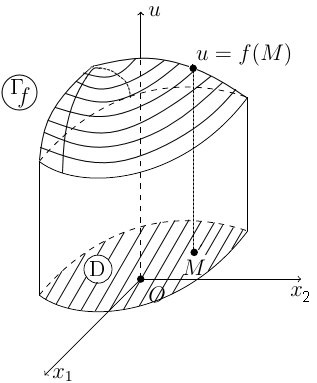
\includegraphics[scale=0.7]{img/2_2.jpg}
\end{center}
Для больших размерностей $n \in \mathbb{N}$ геометрически для изучения свойств ФНП используют линии (поверхности) уровня, т.е. (n-1)-мерные множества, определяемые в силу \eqref{eq:f_n} неявным уравнением $f(x) = C = const \in \mathbb{R}$, где $x \in D \subset \RN$.

Например, для Ф3П $u = x_1^2 + x_2^2 + x_3^2, (x_1, x_2, x_3) \in \mathbb{R}^3$, поверхностями уровня $ x_1^2 + x_2^2 + x_3^2 = $ \\ $ = C  = const \in \mathbb{R}$, будут а) пустое множество $\emptyset$, если $C < 0$, б) точка $O(0, 0, 0)$ для $C = 0$,\\ в) сфера $S_{\sqrt{C}} (\overline{O}) = \{ x_1^2 + x_2^2 + x_3^2 = (\sqrt{c})^2 | (x_1, x_2, x_3) \in \mathbb{R}^3 \}$ с центром в $\overline{O} = (0, 0, 0)$ и радиуса $R = \sqrt{C}$ при $C > 0$.

В дальнейшем будем рассматривать ФНП \eqref{eq:f_n}, определённые не только в некоторой области $D \subset \RN$, но и с множеством определения $D = D(f)$ более сложной структуры, например, имеющей изолированные точки.

В общем случае сходимость ФНП, определённых на соответствующем множестве $D \subset \RN$, рассматривается лишь в точках $x_0 \in \RN$, являющихся предельными для $D$. Для таких точек $M_0 = x_0$ нетрудно видеть, что всегда $\exists M_k \in D, k \in \mathbb{N}$, такая, что $M_k \xrightarrow[k \to \infty]{} M_0$.

Будем говорить, что в метрическом пространстве $(\RN, \rho)$ функция $f(x), x \in D \subset \RN$, сходится к числу $p_0$ при $x \to x_0$, где $x_0$ — предельная точка для $D$, если для $\forall \varepsilon > 0, \exists \delta =$ \\ $= \delta_{\varepsilon} > 0$ такое, что для
\begin{equation}
\label{eq:eps_n}
\forall x \in D, 0 < \rho(x, x_0) \leqslant \delta \Rightarrow \abs{f(x)-p_0} \leqslant \varepsilon\;.
\end{equation}
В этом случае будем писать $f(x) \xrightarrow[x \to x_0]{} p_0 \in \mathbb{R}$, а само число $p_0$ называть пределом $f(x)$ при $x \to x_0$ и обозначать $p_0 = \lim\limits_{x \to x_0} f(x)$.

По аналогии с С-леммой для сходимости n-мерных последовательностей доказывается С-лемма сходимости ФНП: если $\exists C = const \geqslant 0$ такая, что для $\forall \varepsilon > 0, \exists \delta = \delta_{\varepsilon} > 0$, что для $\forall x \in D(f) \subset \RN, 0 < \rho(x, x_0) \leqslant \delta_{\varepsilon} \Rightarrow \abs{f(x) - p_0} \leqslant C \cdot \varepsilon$, то $\exists  \lim\limits_{x \to x_0} f(x) = p_0 \in \mathbb{R}$.

По той же схеме, что и для Ф1П в линейном метрическом пространстве $(\RN, d)$ с евклидовым расстоянием, доказывается критерий Гейне сходимости ФНП: для того, чтобы $f(x) \xrightarrow[x \to x_0]{} p_0 \in \mathbb{R}$, необходимо и достаточно,
чтобы для произвольной последовательности Гейне $M_k \in D(f), k \in \mathbb{N}$, точки $x_0$, т.е. для которой $\forall M_k \ne x_0$ и $M_k \xrightarrow[k \to \infty]{} x_0$, следовало $f(M_k) \xrightarrow[k \to \infty]{} p_0 \in \mathbb{R}$.

В силу этого, как и для Ф1П, на основании соответствующих свойств сходящихся точечных последовательностей в $\RN$, получаем основные свойства
сходящихся ФНП в метрическом пространстве $(\RN, d)$: единственность предела; предел линейной комбинации, произведения и частного сходящихся ФНП. Кроме того в пространстве $(\RN, d)$, которое в дальнейшем, как правило, мы и будем
использовать, справедлива теорема о сжатой ФНП: если для $\forall x \in \dot{V}(x_0) \subset D(f) \cap D(g) \cap D(h)$ имеем $g(x) \leqslant f(x)
\leqslant h(x)$, то в случае, когда $g(x) \xrightarrow[x \to x_0]{} p_0 \in \mathbb{R}$ и $h(x) \xrightarrow[x \to x_0]{} p_0 \in \mathbb{R}$ имеем
$\exists  \lim\limits_{x \to x_0} f(x) = p_0 \in \mathbb{R}$.


\begin{example}
	Рассмотрим в метрическом пространстве $(\RN, d)$ функцию
	\begin{equation*}
	f(x) = \frac{x_1^4 + x_2^4 + \ldots + x_n^4}{x_1^2 + x_2^2 + \ldots + x_n^2}, \text{ где $\forall x = (x_1, x_2, \ldots, x_n) \in \RN \setminus {\{\bar{0}\}}$}.
	\end{equation*}

	Для $\forall x \ne \bar{0} = (0, 0, \ldots, 0) \in \RN \Rightarrow$
	\begin{equation*}
	0 \leqslant f(x) = \sum_{k = 1}^{n} \dfrac{x_k^4}{(x_1^2 + \ldots + x_{k-1}^2) + x_k^2 + (x_{k+1}^2 + \ldots + x_n^2)} \leqslant \sum_{k = 1}^{n} \dfrac{x_k^4}{x_k^2} = \sum_{k = 1}^{n} x_k^2 = h(x).
	\end{equation*}

	Отсюда в силу того, что
	\begin{equation*}
	h(x) = (x_1^2 + x_2^2 + \ldots + x_n^2) \xrightarrow[\forall x_k \to 0]{} 0,
	\end{equation*}
	получаем на основании теоремы о пределе сжатой ФНП, что $\exists \lim\limits_{x \to \bar{0}} f(x) = 0$.
\end{example}

Так же, как и для Ф1П, показывается, что если ФНП $f(x)$ сходится в предельной точке $x_0 \in
\RN$, то $f(x)$ ограничена в некоторой окрестности $\dot{V} (x_0) \subset D(f)$, т.е. $\exists C_0 = const \geqslant 0$ такая, что для $\forall x \in \dot{V}(x_0) \Rightarrow \abs{f(x)} \leqslant C_0$ (локальная ограниченность сходящихся ФНП).

По аналогии с n-мерными б.м.п. определяют бесконечно малые ФНП при $x \to x_0$, т.е. n-мерные функции $f(x)$, для которых $\exists \lim\limits_{x \to x_0} f(x) = 0$.

Как и для Ф1П обосновываются соответствующие свойства n-мерных б.м.ф. (линейная комбинация n-мерных б.м.ф. с ограниченными коэффициентами является б.м.ф., произведение n-мерных б.м.ф. будет б.м.ф. и, в частности, произведение n-мерной б.м.ф. на ограниченную ФНП будет б.м.ф.).

В дальнейшем ФНП \eqref{eq:f_n} будем называть бесконечно большой (Б.Б.Ф.) при $x \to x_0$ в метрическом пространстве $(\RN, \rho)$, если для $\forall \varepsilon > 0$ $\exists \delta = \delta_{\varepsilon} > 0$ такое, что для $\forall x \in D(f),$ \\ $0 < \rho(x, x_0) \leqslant \delta \Rightarrow \abs{f(x)} \geqslant \varepsilon$. В этом случае будем писать $f(x) \xrightarrow[x \to x_0]{} \infty$ или $\exists  \lim\limits_{x \to x_0} f(x) = \infty$.

Среди n-мерных Б.Б.Ф. выделяют положительные Б.Б.Ф. и отрицательные Б.Б.Ф.:
\begin{enumerate}
	\item $f(x) \xrightarrow[x \to x_0]{} +\infty \Leftrightarrow $ для $\forall \varepsilon > 0$ $\exists \delta = \delta_{\varepsilon} > 0$ такое, что для $\forall x \in D(f),$  $0 < \rho(x, x_0) \leqslant \delta \Rightarrow$ $\Rightarrow f(x) \geqslant \varepsilon$.
	\item $f(x) \xrightarrow[x \to x_0]{} -\infty \Leftrightarrow $ для $\forall \varepsilon > 0$ $\exists \delta = \delta_{\varepsilon} > 0$ такое, что для $\forall x \in D(f),$  $0 < \rho(x, x_0) \leqslant \delta \Rightarrow$ $\Rightarrow f(x) \leqslant -\varepsilon$.
\end{enumerate}

\newpage

Кроме рассмотренных бесконечных пределов в конечных предельных точках, рассматривают конечные пределы ФНП на бесконечности, а именно $\lim\limits_{x \to \infty} f(x) = p_0 \in \mathbb{R} \Leftrightarrow$ для $\forall \varepsilon > 0$ $\exists \delta = \delta_{\varepsilon} > 0$ такое, что для $\forall x \in D(f),$ $\rho(x, \bar{0}) \geqslant \delta \Rightarrow \abs{f(x) - p_0} \leqslant \varepsilon$.

В данном случае, в отличие от Ф1П, при $n \geqslant 2$ для $x \in \RN$ не рассматривают отдельно  $x \to + \infty$ или $x \to - \infty$.

Используя бесконечные пределы и пределы на бесконечности, определяют смешанные пределы ФНП.
\begin{enumerate}
	\item $\lim\limits_{x \to \infty} f(x) = +\infty \Leftrightarrow$ для $\forall \varepsilon > 0$ $\exists \delta = \delta_{\varepsilon} > 0$ такое, что для $\forall x \in D(f),$ $\rho(x, \bar{0}) \geqslant \delta \Rightarrow$ $\Rightarrow f(x) \geqslant \varepsilon$.
	\item $\lim\limits_{x \to \infty} f(x) = -\infty \Leftrightarrow$ для $\forall \varepsilon > 0$ $\exists \delta = \delta_{\varepsilon} > 0$ такое, что для $\forall x \in D(f),$ $\rho(x, \bar{0}) \geqslant \delta \Rightarrow$ $\Rightarrow f(x) \leqslant -\varepsilon$.
	\item $\lim\limits_{x \to \infty} f(x) = \infty \Leftrightarrow$ для $\forall \varepsilon > 0$ $\exists \delta = \delta_{\varepsilon} > 0$ такое, что для $\forall x \in D(f),$ $\rho(x, \bar{0}) \geqslant \delta \Rightarrow$ $\Rightarrow \abs{f(x)} \geqslant \varepsilon$.
\end{enumerate}

\subsection{Реализация для Ф2П и Ф3П}
Рассмотрим вначале линейное метрическое пространство $ (\mathbb{R}^2, d) $ с евклидовым расстоянием, снабжённое прямоугольной декартовой системой координат $ Oxy $,
в которой элементы $ \mathbb{R}^2 $ будем обозначать через $ M(x; y) $, где
$ x \in \mathbb{R} $ и $ y \in \mathbb{R} $. В этом случае, как отмечалось ранее, для Ф2П $ u=f(M)=f(x,y) $ с областью определения $ D \subset \mathbb{R}^2 $ графику \plot{f}
соответствует некоторая поверхность в $ \mathbb{R}^3 $. Линиями уровня для рассматриваемой Ф2П в плоскости $ Oxy $ являются множества точек $ M(x, y) \in D $, удовлетворяющих неявным уравнениям
$ f(x, y) = $ \\
$ = \const \in \mathbb{R} $ и получаемые как проекция на плоскость $ Oxy $ пересечения $ \text{Г}_f $ с горизонтальными плоскостями $ u = const $.

\begin{example}
    Пусть $ u = x^2 + y^2 $, где $ (x,y) \in \mathbb{R}^2 $. Для линий уровня $ u = C = \const  \in \mathbb{R} $ имеем неявное уравнение $ x^2 + y^2 = C $, что для $ C < 0 $ даёт пустое
    множество $ \varnothing $, для $ C = 0 $ имеем одну точку $ O(0,0) $, а для  $ C > 0 $ получаем в плоскости $ Oxy $ концентрические окружности
    $ x^2 + y^2 = \left(\sqrt{C}\right)^2 $ с общим центром $ O(0; 0) $ и радиусов $ R = \sqrt{C} \in \mathbb{R} $.
    Здесь все эти линии уровня получаются как проекция пересечения на плоскость $ Oxy $ графика \plot{f}, являющегося в данном случае соответствующим эллиптическим параболоидом
    в $ \mathbb{R}^3 $, с горизонтальными плоскостями $ u =  C \in \mathbb{R} $.

    \begin{center}
        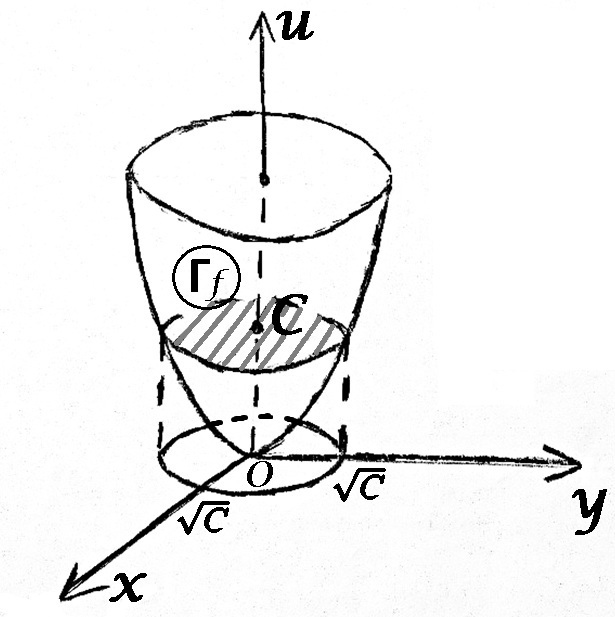
\includegraphics[scale=0.4]{img/2_3.jpg}
    \end{center}
\end{example}

Если $ f(x,y) $ определена в некоторой выколотой окрестности \r{V}$(M_0) \subset D(f) $ предельной для множества $ D(f) \subset \mathbb{R}^2 $ точки $ M_0 (x_0, y_0) $, то в этом случае
общий предел $ p_0 = \lim\limits_{M \to M_0} f(M) $ называют двойным и обозначают
\begin{equation}
    \label{lect02:doubleLimit}
    p_0 = \limlim{x \to x_0}{y \to y_0} f(x, y)
\end{equation}

Кроме \eqref{lect02:doubleLimit}, для Ф2П рассматривают повторные пределы
\begin{equation}
    \label{lect02:limlimXY}
    p_1 = \lim\limits_{x \to x_0} \left( \lim\limits_{y \to y_0} f(x,y) \right)
\end{equation}

$ \;\;\;\;\;\;\;\;\;\;\;\;\;\;\;\;\;\;\;\;\;\;\;\;\;\;\;\;\;\;\;\;\;\;\;\;\;\;\;\;\; $ и

\begin{equation}
    \label{lect02:limlimYX}
    p_2 = \lim\limits_{y \to y_0} \left( \lim\limits_{x \to x_0} f(x,y) \right) ,
\end{equation}

а также частные пределы, когда независимые переменные $ x $ и $ y $ стремятся соответственно к $ x_0 $ и $ y_0 $ не произвольным образом, а специальным, например, по некоторой плоской линии
$ l \subset D(f) $, проходящей через точку $ M_0(x_0, y_0) $.

Можно показать, что если для Ф2П существует двойной предел \eqref{lect02:doubleLimit} и существуют повторные пределы \eqref{lect02:limlimXY} и \eqref{lect02:limlimYX},
то они равны между собой. Аналогичное утверждение верно и для частных пределов Ф2П.

\begin{examples}
    \item Рассмотрим Ф2П:
    $ \;\;\;\;\;\;\;\;\;\;\;\;
        f(x,y) = \dfrac{x^2 + y^2}{\abs{x} + \abs{y}}, \;\; (x, y) \neq (0, 0).
    $\\
    Имеем:
    \begin{equation*}
    \exists \; p_1 = \lim\limits_{x \to 0} \left( \lim\limits_{y \to 0} \dfrac{x^2 + y^2}{\abs{x} + \abs{y}} \right) \overset{x \neq 0}{=}
    \lim\limits_{x \to 0} \dfrac{x^2}{\abs{x}} = \lim\limits_{x \to 0} \abs{x} = 0 \in \mathbb{R} .
    \end{equation*}

    Аналогично, в силу симметрии $ f(x, y) $ по $ x $ и $ y $, получаем:
    \begin{equation*}
        \exists \; p_2 =
        \lim\limits_{y \to 0} \left( \lim\limits_{x \to 0} \dfrac{x^2 + y^2}{\abs{x} + \abs{y}} \right)  =
        0 \in \mathbb{R}.
    \end{equation*}

    Поэтому, если
   \begin{equation*}
        \exists \; p_0 = \limlim{x \to 0}{y \to 0} f(x,y),
   \end{equation*}
   то $ p_0 = p_1 = p_2 = 0$. В данном случае в силу неравенств
   \begin{equation*}
       0 \leqslant f(x,y) = \dfrac{x^2}{\abs{x} + \abs{y}} + \dfrac{y^2}{\abs{x} + \abs{y}} \leqslant
       \dfrac{x^2}{\abs{x}} + \dfrac{y^2}{\abs{y}} = \left( \nullFrac \abs{x} + \abs{y} \nullFrac \right) \xrightarrow[\substack{x \to 0 \\ y \to 0}]{} 0
   \end{equation*}
    на основании  теореме о пределе сжатой ФНП следует, что, действительно, $ p_0 = 0 $.

    \item Пусть  $ f(x,y) = x \cos \dfrac{1}{y} + y \cos \dfrac{1}{x}$, где $ x \neq 0 $ и $ y \neq 0 $.

    Так как при $ x \neq 0  \Rightarrow \nexists \lim\limits_{y \to 0} \left( x \cos \dfrac{1}{y} \right) $, то
    \begin{equation*}
        \nexists \; p_1 =
        \lim\limits_{x \to 0} \left( \lim\limits_{y \to 0} \left( x \cos \dfrac{1}{y} + y \cos \dfrac{1}{x} \right) \right)
        = \lim\limits_{x \to 0} \left( \lim\limits_{y \to 0} x \cos \dfrac{1}{y} \right) .
    \end{equation*}

    Аналогично получаем, что
    \begin{equation*}
    \nexists \; p_2 =
    \lim\limits_{y \to 0} \left( \lim\limits_{x \to 0} \left( x \cos \dfrac{1}{y} + y \cos \dfrac{1}{x} \right) \right) .
    \end{equation*}

    В то же время здесь
    \begin{equation*}
        \exists \; p_0 = \limlim{x \to 0}{y \to 0} f(x,y) = 0,
    \end{equation*}
    так как для $ \forall \; x \neq 0 $ и $ \forall \; y \neq 0 $ следует
    \begin{equation*}
        0 \leqslant \abs{f(x,y)} \leqslant \abs{x} \abs{\cos \dfrac{1}{y}} + \abs{y} \abs{\cos \dfrac{1}{x}} \leqslant
        \left( \nullFrac \abs{x} + \abs{y} \nullFrac \right) \xrightarrow[\substack{x \to 0 \\ y \to 0}]{} 0.
    \end{equation*}

    \item Для Ф2П $ \;\;\;\;\;\;\;\;\;\;\;\;\;\; $
    $ f(x,y)  = \dfrac{x^2 y}{x^4+y^2}, (x,y) \neq (0,0)  $

    имеем:
    \begin{equation*}
        \exists \; p_1 = \lim\limits_{x \to 0} \left(\lim\limits_{y \to 0} \dfrac{x^2 y}{x^4+y^2} \right)
        \;\overset{x \neq 0}{=}\;
        \lim\limits_{x \to 0} \dfrac{0}{x^4} = 0,
    \end{equation*}
    \begin{equation*}
        \exists \; p_2 = \lim\limits_{y \to 0} \left(\lim\limits_{x \to 0} \dfrac{x^2 y}{x^4+y^2} \right)
        \;\overset{y \neq 0}{=}\;
        \lim\limits_{y \to 0} \dfrac{0}{y^2} = 0,
    \end{equation*}.

    Хотя здесь $ p_1 = p_2 = 0 $, но в то же время
    \begin{equation*}
         \nexists \; p_0 = \limlim{x \to 0}{y \to 0} \dfrac{x^2 y}{x^4+y^2}
    \end{equation*}

    Для обоснования этого рассмотрим частный предел по параболе $ y = x^2 $, проходящей через точку $ (0, 0) $:
    \begin{equation*}
       p = \limlim{x \to 0}{y = x^2 \to 0}
     %   p = \lim\limits_{
     %       \begin{cases}
     %           x \to 0 \\
     %           y = x^2 \to 0
     %       \end{cases}
     %   }
        f(x,y) = \lim\limits_{x \to 0} \dfrac{x^4}{x^4 + x^4} = \dfrac{1}{2}
    \end{equation*}
    Так как $ p = \dfrac{1}{2} \neq 0 $, то $ \nexists \; p_0 $.
\end{examples}

Аналогичные результаты справедливы и для Ф3П в метрическом пространстве $ (\mathbb{R}^3, d) $ с прямоугольной декартовой системой координат $ Oxyz $. В данном случае также кроме общего (тройного) предела
\begin{equation*}
    p_0 = \limlimlim{x \to x_0}{y \to y_0}{z \to z_0} f(x, y, z)
\end{equation*}
рассматривается шесть повторных пределов, одним из которых, например, является
\begin{equation*}
    p_1 = \lim\limits_{x \to x_0} \left( \lim\limits_{y \to y_0}
    \left( \lim\limits_{z \to z_0} f(x, y, z) \right) \right)
\end{equation*}
Здесь также, если существуют повторные пределы Ф3П и существует тройной предел, то все они равны между собой. Аналогично и для частных пределов Ф3П.
\newpage

\begin{examples}
    \item Пусть
    $\;\;\;\;\;\;\;\;\;\;\;\;\;\;\;\;\;\;\;\;\;\;\;\;\;\;\;\;\;\;\;\;\;\;\;\;\;\;\;\;\;\;\;$
    $ f(x, y, z) = \dfrac{x^2+y^2+z^2}{e^{x+y+z}}. $

    Разделяя переменные, имеем
    \begin{equation*}
    \begin{split}
    & p_0 = \limlimlim{x \to +\infty}{y \to +\infty}{z \to +\infty} f(x, y, z) = \limlimlim{x \to +\infty}{y \to +\infty}{z \to +\infty} \left( \dfrac{x^2}{e^x} \cdot \dfrac{1}{e^y}\cdot \dfrac{1}{e^z} \right) + \limlimlim{x \to +\infty}{y \to +\infty}{z \to +\infty} \left( \dfrac{1}{e^x} \cdot \dfrac{y^2}{e^y}\cdot \dfrac{1}{e^z} \right) + \limlimlim{x \to +\infty}{y \to +\infty}{z \to +\infty} \left( \dfrac{1}{e^x} \cdot \dfrac{1}{e^y}\cdot \dfrac{z^2}{e^z} \right) = \\
    & =
    \begin{sqcases}
    	\text{а) } \dfrac{1}{e^t} \xrightarrow[t \to +\infty]{} 0
        \;\;\;\;\;\;\;\;\;\;\;\;\;\;\;\;\;\;\;\;\;\;
        \;\;\;\;\;\;\;\;\;\;\;\;\;\;\;\;\;\;\;\;\;\;
        \;\;\;\;\;\;\;\;\;\;\;\;\;\;\;\;\;\;\;\;
        \\
    	\text{б) } \lim\limits_{t \to +\infty} \dfrac{t^2}{e^t} = \left[ \dfrac{\infty}{\infty}\right] \overset{\circled{\text{Л}}}{=} \lim\limits_{t \to +\infty} \dfrac{2t}{e^t} = \left[ \dfrac{\infty}{\infty}\right] \overset{\circled{\text{Л}}}{=} \lim\limits_{t \to +\infty} \dfrac{2}{e^t} = 0
    \end{sqcases} = 0.
    \end{split}
    \end{equation*}
    \item  Рассмотрим
    \begin{equation*}
    p_0 = \limlimlim{x \to +0}{y \to +0}{z \to +0} (x+y+z)^{xyz}.
    \end{equation*}
    Для одного из повторных пределов имеем
    \begin{equation*}
    \exists p_1 = \lim\limits_{x \to +0}\lim\limits_{y \to +0}\lim\limits_{z \to +0} (x+y+z)^{xyz} = \lim\limits_{x \to +0}\lim\limits_{y \to +0} (x+y)^0 \;\;\overset{x > 0, y > 0}{=} \;\; \lim\limits_{x \to +0} 1 = 1 \in \mathbb{R}.
    \end{equation*}
    Поэтому, если $\exists p_0 \in \mathbb{R}$, то $p_0 = p_1 = 1$. Покажем, что действительно $\exists p_0 = 1$. Во-первых, т.к. $(x+y+z) \xrightarrow[\substack{x \to +0 \\ y \to +0 \\ z \to +0}]{} +0$, то в достаточно малой соответствующей окрестности предельной точки $O(0;0;0)$ будем иметь $0 \leqslant x + y + z \leqslant 1$, и, значит, для этих $x > 0, y > 0$ и $z > 0 \Rightarrow (x+y+z)^{xyz} \leqslant 1$.

    Во-вторых, используя неравенство между средним арифметическим и средним геометрическим трёх положительных чисел, получаем
    \begin{equation*}
    \dfrac{x+y+z}{3} \geqslant \sqrt[3]{xyz} \Rightarrow (x+y+z)^{xyz} \geqslant \left(3 \sqrt[3]{xyz}\right)^{xyz}.
    \end{equation*}
    Отсюда при $x \to +0, y \to +0, z \to +0$ следует
    \begin{equation*}
	    \left(3 \sqrt[3]{xyz}\right)^{xyz} \leqslant (x+y+z)^{xyz} \leqslant 1.
    \end{equation*}
    Делая замену $t = xyz \xrightarrow[\substack{x \to +0 \\ y \to +0 \\ z \to +0}]{} +0$ имеем
    \begin{equation*}
    \begin{split}
    & \exists \limlimlim{x \to +0}{y \to +0}{z \to +0} \left(3 \sqrt[3]{xyz}\right)^{xyz} =  \lim\limits_{t \to +0} \left(27t\right)^{\frac{t}{3}} = \begin{sqcases} 0^0 \end{sqcases} = 
    e^{\lim\limits_{t \to +0} \dfrac{t \ln (27t)}{3} } = e^{\lim\limits_{t \to +0} \dfrac{ln (27t)}{3t^{-1}} } = \left[ \dfrac{\infty}{\infty}\right] \overset{\circled{\text{Л}}}{=} \\
    & \overset{\circled{\text{Л}}}{=} e^{\lim\limits_{t \to +0} \dfrac{\frac{1}{t}}{-3t^{-2}} } = e^{\lim\limits_{t \to +0} \left(-\dfrac{t}{3} \right)} = e^0 = 1.
    \end{split}
    \end{equation*}
    Поэтому в силу теоремы о пределе сходящейся ФНП получим, что действительно ${\exists p_0 = 1}$.

    Отметим, что при $n > 2$ для ФНП, в отличие от Ф1П, аналога правил Лопиталя вычисления пределов нет.
\end{examples}

\subsection{Непрерывные ФНП}
Рассмотрим ФНП $u = f(x) = f(x_1, x_2, \ldots, x_n),$ множеством определения которой является область (открытое связное множество) $D \subset \RN$. Эта ФНП называется непрерывной в точке $M_0 = (x_{01}, x_{02}, \ldots, x_{0n}) \in D$, если
\begin{equation}
\label{27}
\exists \lim\limits_{M \to M_0} f(M) = f(M_0).
\end{equation}
На $\varepsilon-\delta$ языке \eqref{27} означает, что для $\forall \varepsilon > 0 \ \exists \delta = \delta_\varepsilon > 0$ такое, что для ${\forall M = (x_1, \ldots, x_n) \in  D}$, $ d (M, M_0) \leqslant \delta$, имеем
\begin{equation}
\label{28}
\abs{f(M) - f(M_0)} \leqslant \varepsilon.
\end{equation}
Отличие \eqref{28} от общего определения предела ФНП состоит, во-первых, в том, что $f(x)$ определена в точке $M_0 \in D$, и, во-вторых, заранее известно предельное значение $p_0 = \\ = \lim\limits_{M \to M_0} f(M) = f(M_0)$.

В дальнейшем наряду с точечными обозначениями аргументов для ФНП будем использовать и векторные записи.

В случае, когда $D$ не является областью, а, например, имеет изолированные точки, рассматриваемая ФНП
по определению считается непрерывной в этих точках. Если у $D$ есть граничные точки $x_0 \in D$, то
здесь рассматривается непрерывность вдоль множества $D$, т.е. $f(x)$ - непрерывна в $x_0 \in \partial D$,
если $\exists 
%\lim\limits_{    \begin{dcases}    x \to x_0 \\ x \in \partial D\end{dcases}    }
\limlim{x \to x_0}{x \in \partial D}
    f(x) = f(x_0)$.

Функцию ФНП будем считать непрерывной на множестве $D \subset \RN$, если она непрерывна в каждой
точке из $D$. При этом для граничных точек из $D$ подразумевается соответствующая односторонняя
непрерывность. Множество всех непрерывных функций на $D$ будем обозначать $C(D)$. Как и для Ф1П,
доказывается, что для функций, непрерывных на $D \subset \RN$ имеем:
\begin{enumerate}
  \item Линейная комбинация конечного числа непрерывных ФНП на $ D $ с постоянными коэффициентами будет непрерывной ФНП на $ D $.
  \item Произведение непрерывных ФНП на $D$ будет непрерывной ФНП на $D$.
  \item Частное двух непрерывных ФНП на $D$ будет непрерывной ФНП во всех точках из $D$, где знаменатель
	не нулевой.
\end{enumerate}

Кроме того, как и для Ф1П, имеем следующие локальные свойства непрерывных ФНП:
\begin{enumerate}[label=\asbuk*)]
  \item Локальная ограниченность.\\
	Если $f(x)$ непрерывна в $x_0 \in D(f)$, то $\exists V(x_0) \subset D(f)$, такая, что для
	$\forall x \in V(x_0) \Rightarrow \abs{f(x)} \leqslant C = \const$.
  \item Стабилизация знака непрерывной ФНП.\\
	Если $f(x)$ непрерывна в $x_0 \in D(f)$ и $f(x_0) \neq 0$, то
	\begin{equation*}
		\begin{split}
		  &\exists V(x_0) \subset D(f), \text{ такая, что для } \forall x \in V(x_0) \Rightarrow
		  \sgn f(x) = \sgn f(x_0), \text{ т.е. если } f(x_0) > 0 \\
		  & (f(x_0) < 0),\text{ то и } f(x) > 0 \; (f(x) < 0) \text{ для } \forall x \in V(x_0).
		\end{split}
	\end{equation*}
\end{enumerate}

\begin{theorem}[о непрерывности композиции ФНП]
	Если $n$ функций $g_k(t), k = \overline{1, n}$ от $m$ переменных $t = (t_1, \ldots, t_m) \in D(g) \subset \mathbb{R}^m$ непрерывны во внутренней точке ${t_0 = (t_{01}, \ldots, t_{0m}) \in D(g)}$, где
	$g(t) = (g_1(t), \ldots, g_n(t))$, и функция $ f(x) $ от $n$ переменных ${x = (x_1, \ldots , x_n) \in D(f) \subset \RN}$ непрерывна во внутренней точке $x_0 = g(t_0) \in D(f)$, то в случае существования
	композиции
	\begin{equation}
		\label{eq:2-fg-composition}
		h(t) = (f \circ g)(t) = f(g(t)) = f(g_1(t), \ldots, g_n(t)),
	\end{equation}
	в соответствующих окрестностях $ \overset{ \sim }{V} (t_0) $ и $ V (x_0) $ точек $t_0$ и $x_0$, сложная функция $h(t)$ будет непрерывна в точке $t_0$.
\end{theorem}
\begin{proof}
	Из непрерывности $f(x)$ в точке $x_0 = g(t_0)$ следует, что для
	\begin{equation}
		\label{eq:2-composition-theorem}
		\forall \varepsilon > 0, \exists \delta > 0, \text{ такое, что для } \forall x \in V(x_0)
		\cap D(f), d(x, x_0) \leqslant \delta \Rightarrow \abs{f(x) - f(x_0)} \leqslant \varepsilon.
	\end{equation}
	Аналогично из того, что $\forall g_k(t), k = \overline{1, m}$ непрерывна в точке $t_0$ следует,
	что для
	\begin{equation*}
		\tilde{\varepsilon} = \dfrac{\varepsilon}{\sqrt{n}} > 0, \exists \tilde{\delta_k} > 0,
		\text{ такое, что для } \forall t \in \overset{ \sim }{V} (t_0) \cap D(g_k), d(t, t_0) \leqslant \tilde{\delta_k}
		\Rightarrow \abs{g_k(t) - g_k(t_0)} \leqslant \tilde{\varepsilon}.
	\end{equation*}
	Выбирая $\delta_{\varepsilon} = \min\limits_{1 \leqslant k \leqslant n}{\set{\tilde{\delta_k}}} > 0$ и
	учитывая, что если $d(t, t_0) \leqslant \delta_{\varepsilon}$, то $d(t, t_0) \leqslant  \tilde{\delta_k}, \forall k = \overline{1, n}$, и, значит, $\abs{g_k(t) - g_k(t_0)} \leqslant \tilde{\varepsilon}, \forall k = \overline{1, n}$, во-первых, имеем:
	\begin{equation*}
		\max\limits_{1 \leqslant k \leqslant n}\abs{g_k(t) - g_k(t_0)} \leqslant \tilde{\varepsilon},
	\end{equation*}
	и, во-вторых, получаем:
	\begin{equation*}
		\begin{split}
			&d(g(t), g(t_0)) = \sqrt{\sum\limits_{k = 1}^n(g_k(t) - g_k(t_0))^2} \leqslant
			\sqrt{\sum\limits_{k = 1}^n(\max\limits_{1 \leqslant k \leqslant n}\abs{g_k(t) - g_k(t_0)})^2}
			\leqslant\\
			&\leqslant \sqrt{\sum\limits_{k=1}^n\tilde{\varepsilon}^2} = \tilde{\varepsilon}\sqrt{n}
			= \dfrac{\varepsilon}{\sqrt{n}}\cdot\sqrt{n} = \varepsilon.
		\end{split}
	\end{equation*}
	Отсюда следует, что для
	\begin{equation*}
		\begin{split}
			\forall \varepsilon > 0, \exists \delta_{\varepsilon} > 0, \text{ такое, что для } \forall
			t \in \overset{ \sim }{V} (t_0) \cap D(g), d(t, t_0) \leqslant \delta_{\varepsilon} \Rightarrow \\
			\Rightarrow
			\abs{h(t) - h(t_0)} = \abs{f(g(t)) - f(g(t_0))} = \abs{f(x) - f(x_0)} \leqslant \varepsilon.
		\end{split}
	\end{equation*}
\end{proof}

\begin{consequence}[о пределе композиции ФНП]
	Пусть $\exists \lim\limits_{t \to t_0}g_k(t) = p_k \in \mathbb{R}, k = \overline{1, n}$, где \\
	${t = (t_1, \ldots, t_m) \in D(g) \subset \R{m}}$, ${g(t) = (g_1(t), \ldots, g_n(t))}$, а
	${t_0 = (t_{01}, \ldots, t_{0m}) \in \R{m}}$ - предельная точка $D(g)$. Если функция $f(x)$
	непрерывна во внутренней точке $x_0 = (p_1, \ldots, p_n) \in D(f) \subset \R{n}$, то в случае
	существования композиции $h(t) = f(g(t))$ в соответствующих окрестностях точек $t_0$ и $x_0$
	имеем:
	\begin{equation*}
		\exists \lim\limits_{t \to t_0}h(t) = \lim\limits_{t \to t_0}f(g(t)) =
		\begin{sqcases}
			x = g(t) \xrightarrow[t \to t_0]{} x_0 = (p_1, \ldots, p_n)
		\end{sqcases}
		= \lim\limits_{x \to x_0}f(x) = f(x_0).
	\end{equation*}
    
    \begin{proof}
        Как и для Ф1П, рассмотрим доопределённую функцию
        \begin{equation*}
        G(t) = \begin{cases}
        g(t), \;\; t \neq t_0,\\
        x_0, \;\;\;\; t = t_0.
        \end{cases}
        \end{equation*}
        Учитывая, что для $g(t) = (g_1(t), \ldots, g_m(t))$ каждая функция $g_k(t) \xrightarrow[t \to t_0]{} p_k \in \mathbb{R}$, получаем, что
        \begin{equation*}
        \exists \lim\limits_{t \to t_0}G(t) \overset{t \neq t_0}{=} \lim\limits_{t \to t_0} g(t) = (\lim\limits_{t \to t_0} g_1(t), \ldots, \lim\limits_{t \to t_0} g_n(t))
        = (p_1, \ldots , p_n) = x_0 = G(t_0),
        \end{equation*}
        т.е. $G(t)$ непрерывна в соответствующей окрестности точки $t_0$. Тогда в случае существования
        композиции функция $H(t) = f(G(t))$ будет непрерывной. Поэтому
        \begin{equation*}
        \exists \lim\limits_{t \to t_0}h(t) = \lim\limits_{t \to t_0}f(g(t)) \overset{t \neq t_0}{=}
        \lim\limits_{t \to t_0}f(G(t)) = \lim\limits_{t \to t_0}H(t) = H(t_0) = f(G(t_0)) = f(x_0).
        \end{equation*}
    \end{proof}
    	
\end{consequence}

\begin{note}
	Как и в случае Ф1П, полученный результат даёт возможность использовать метод замены переменных
	при вычислении пределов сложных ФНП.
\end{note}

\begin{theorem}[о промежуточных значениях непрерывных на связном множестве ФНП]
	Пусть $f(x) \in C(D)$, где $D \subset \R{n}$. Если $D$-связное множество в $\R{n}$, то в случае,
	когда $f(x)$ принимает значения $A$ и $B$, т.е. когда
  $   \exists a, b \in D \Rightarrow f(a) = A, f(b) =  B, $
	то тогда $f(x)$ принимает на $D$ любое промежуточное значение $C \in \mathbb{R}$, лежащее между
	$A$ и $B$.
\end{theorem}

\begin{proof}
	Так как $D$-связное множество в $\R{n}$, то любые его точки $a, b \in D \subset \R{n}$ можно
	соединить гладкой линией $l \subset D$, имеющей параметризацию
	\begin{equation}
		\label{eq:2-intermediate-value}
		l : x = x(t) = (x_1(t), \ldots, x_n(t)) \in D, 
	\end{equation}
    %\begin{equation*}
    $
        \text{ где } 
        \forall x_k(t)
        \text{ - непрерывные функции от } t, k = \overline{1, n}.
    $   
    %\end{equation*}
    
	Взяв произвольные $a, b \in D$, найдём $t_1, t_2 \in \mathbb{R}$, такие, что
	\begin{equation*}
		\begin{cases}
			a = x(t_1),\\
			b = x(t_2).
		\end{cases}
	\end{equation*}
    
	По теореме о непрерывности композиции получаем, что
	$ %\begin{equation*}
		h(t) = f(x(t)) = f(x_1(t), \ldots, x_n(t)),
	$ %\end{equation*}
	в силу \eqref{eq:2-intermediate-value}, будет непрерывна на $l$ для $\forall \; t$, лежащих
	между $t_1$ и $t_2$.

	Отсюда, учитывая, что ${A = f(x(t_1)) = f(a)}$, ${B = f(x(t_2)) = f(b)}$, получаем, что
	непрерывная функция $h(t)$, принимающая значения $A$ и $B$, будет принимать и любое значение
	$C \in \mathbb{R}$, лежащее между $A$ и $B$, т.е.
    $ \exists t_0 \text{ между } t_1 \text{ и } t_2 \text{, такое, что } h(t_0) = C. $
    
	Полагая $x_0 = x(t_0) \in l$, будем иметь $f(x_0) = f(x(t_0)) = h(t_0) = C.$
\end{proof}
$  $\newline
\begin{note}
	Доказанная теорема показывает, что для ФНП, непрерывной на связном множестве, её множеством
	значений будет являться некоторый промежуток $E(f) = \abs{A_0, B_0}$, который является связным
	множеством в $\mathbb{R}$.
\end{note}

\begin{consequence}[о прохождении непрерывной ФНП через ноль]
	Если $f(x)$ непрерывна на связном множестве $D \in \R{n}$ и $\exists a, b \in D$, такие, что
	$f(a)f(b) < 0$, то $\exists \; x_0 \in D$, для которого $f(x_0) = 0$.
\end{consequence}

\textit{Доказательство}
	проводится по той же схеме, что и для Ф1П и следует из того, что, если числа $A = f(a)$ и $B = f(b)$
	имеют разные знаки, то для $C_0 = 0$, лежащей между $A$ и $B$, получаем, что $\exists x_0 \in D$,
	такое, что $f(x_0) = C_0 = 0$.\\\\

Кроме локальных свойств ФНП, для непрерывных ФНП справедливы соответствующие глобальные свойства,
например, теоремы Вейерштрасса и Кантора для ФНП.

\begin{statementUncoloned}{Теорема Вейерштрасса}(о достижении непрерывной на компакте ФНП своих экстремальных значений)
    
    \textit{Если $f(x)$ непрерывна на компакте $D \subset \R{n}$, то $\exists x_1, x_2 \in D$,для которых}
    \begin{equation}
        \label{eq:2-vejershtrass-theorem}
        \begin{cases}
            m_0 = \min\limits_{x \in D} f(x) = f(x_1),\\
            M_0 = \max\limits_{x \in D} f(x) = f(x_2).
            \end{cases}
    \end{equation}
\end{statementUncoloned} 

\begin{proof}
	По теореме о гранях получаем, что $\exists M_0 = \sup\limits_{x \in D}f(x)$. Покажем, что $M_0$ конечно.
	Предполагая, что $M_0 = +\infty$, получим, что для
	\begin{equation*}
		\forall k \in \mathbb{N}, \exists x_k = (x_{k1}, \ldots, x_{kn}) \in D \subset \R{n} \Rightarrow
		f(x_k) \geqslant k.
	\end{equation*}
	В силу принципа выбора для ФНП из ограниченной последовательности $(x_k) \in D$ можно выбрать
	сходящуюся подпоследовательность. Будем считать для простоты, что такой подпоследовательностью является
	сама $(x_k)$, т.е. $\exists\lim\limits_{k \to \infty}x_k = x_0$. Из того, что $D$ - компакт
	(ограниченное замкнутое множество), следует, что $x_0 \in D$. 
    
    По критерию Гейне в силу
	непрерывности $f(x)$ имеем
	\begin{equation*}
		f(x_0) = f(\lim\limits_{k \to \infty}x_k) = \lim\limits_{k \to \infty} f(x_k) =
		\begin{sqcases}
			f(x_k) \geqslant k \Rightarrow f(x_k) \xrightarrow[k \to \infty]{} +\infty
		\end{sqcases} = +\infty,
	\end{equation*}
	что противоречит тому, что $x_0 \in D$, и, значит, $f(x_0) \in E(f)$ - конечное значение.
	Поэтому $M_0 \in \mathbb{R}$. 
    
    Предположим, что для $\forall x \in D \Rightarrow f(x) \neq M_0$.
	Тогда функция $g(x) = \dfrac{1}{M_0 - f(x)} > 0$ будет непрерывной на компакте $D$. Поэтому
	в силу предыдущего для неё $\exists \varepsilon_0 = \sup\limits_{x \in D}g(x) \in \mathbb{R}$ и
	$\varepsilon_0 > 0$. Отсюда 
	$ %\begin{equation*}
		\text{для } \forall x \in D \Rightarrow 0 < \dfrac{1}{M_0 - f(x)} = g(x) \leqslant \sup\limits_{x \in D}g(x)
		= \varepsilon_0.
	$ %\end{equation*}
    
	Значит, $M_0 - f(x) \geqslant \dfrac{1}{\varepsilon_0}$, т.е. $f(x) \leqslant M_0 -
	\dfrac{1}{\varepsilon_0}$, и, следовательно, $M_0 = \sup\limits_{x \in D}f(x) \leqslant M_0 -
	\dfrac{1}{\varepsilon_0}$, т.е. $M_0 \leqslant M_0 - \dfrac{1}{\varepsilon_0} \Rightarrow
	\varepsilon_0 < 0$ - противоречие. Поэтому $\exists x_0 \in D$, такое, что $M_0 = f(x_0) =
	\max\limits_{x \in D}f(x)$.

	Для $m_0 = \min\limits_{x \in D}f(x)$ доказательство аналогично.
\end{proof}
\newpage

По той же схеме, что и для Ф1П, определяются равномерно непрерывные ФНП:\\
$f(x)$ - равномерно
непрерывна на $D \subset \R{n}$, если для
\begin{equation*}
	\forall \varepsilon > 0, \exists \delta > 0, \text{ такое, что для } \forall t, s \in D,
	d(t, s) \leqslant \delta \Rightarrow \abs{f(t) - f(s)} \leqslant \varepsilon.
\end{equation*}
В общем случае любая равномерно непрерывная ФНП на $D \subset \R{n}$ будет непрерывна на $D$. Как
и для Ф1П, доказывается теорема Кантора для ФНП: ФНП $f(x)$, непрерывная в компакте
$D \subset \R{n}$, будет равномерно непрерывна на $D$.

    \section{Дифференцируемые ФНП.}

\subsection{Частные производные первого порядка и дифференциал ФНП.}

Пусть $f(x)$ определена в некоторой окрестности $V(x_0) \subset \RN$ точки $x_0 = (x_{01}, x_{02}, \ldots, x_{0n}) \in$ $\in \RN$. Выбирая любое $\Delta x = (\Delta x_1, \Delta x_2, \ldots, \Delta x_n) \in \RN$ такое, что $(x_0 + \Delta x) \in V(x_0)$, рассмотрим приращение $\Delta f(x_0) = f(x_0 + \Delta x) - f(x_0)$ функции $f(x)$ в точке $x_0$, соответствующее приращению $\Delta x \in \RN$ независимой переменной $x \in V(x_0)$.

ФНП $f(x)$ называется \important{дифференцируемой} в точке $x_0$, если $\exists p_k \in \mathbb{R}, k = \overline{1,n}$, такое, что 
\begin{equation}
\label{31}
\Delta f(x_0) = p_1 \Delta x_1 +  p_2 \Delta x_2 + \ldots +  p_n \Delta x_n + \alpha, 
\end{equation}
где $\alpha = o \left(\sqrt{\Delta x_1^2 + \Delta x_2^2 + \ldots + \Delta x_n^2}\right) = o(|\Delta x|)$, т.е. $\exists \lim\limits_{\Delta x \to 0} \dfrac{\alpha}{|\Delta x|} = 0$.

Отметим, что в \eqref{31} конечные величины $p_k, k = \overline{1, n}$, не зависят от выбора допустимых приращений $\Delta x_1, \Delta x_2, \ldots, \Delta x_n$, но могут зависеть от используемой точки $x_0 \in V(x_0) \subset D(f)$. Если $f(x)$ дифференцируема в точке $x_0$, то, выбирая соответствующие частные приращения $\Delta_k x = (0, 0, \ldots, 0, \underbrace{\Delta x_k}_{\text{k-ое место}}, 0, \ldots, 0) \in \RN$ независимой переменной ${x = (x_1, x_2, \ldots, x_n) \in V(x_0)}$ 
для получаемых частных приращений функции $\Delta_k f(x_0) = f(x_0+\Delta_k x) - f(x_0) =$ \\
$= f(x_{01}, x_{02}, \ldots, x_{0k-1}, x_{0k} + \Delta x_k, x_{0k+1}, \ldots, x_{0n}) - f(x_{01}, x_{02}, \ldots, x_{0n})$ в силу \eqref{31} имеем:
\begin{equation}
\label{32}
\Delta_k f(x_0) = p_k \Delta x_k + \alpha_k,
\end{equation}
где $\alpha_k = o(|\Delta x_k|) = o(\Delta x_k), k = \overline{1,n}$. Из \eqref{32} следует, что
\begin{equation}
\label{33}
\exists \lim\limits_{\Delta x_k \to 0} \dfrac{\Delta_k f(x_0)}{\Delta x_k} \overset{\eqref{32}}{=} \lim\limits_{\Delta x_k \to 0} (p_k + \dfrac{o(\Delta x_k)}{\Delta x_k}) = p_k \in \mathbb{R}, k = \overline{1, n}.
\end{equation}

В общем случае конечные величины \eqref{33} называются частными производными первого порядка дифференцируемой в точке $x_0$ функции $f(x)$ и обозначаются
\begin{equation}
\label{34}
\begin{split}
& p_k = \dfrac{\partial f(x_0)}{\partial x_k} \overset{\eqref{32}}{=} \lim\limits_{\Delta x_k \to 0} \dfrac{\Delta_k f(x_0)}{\Delta x_k} = \\
& = \lim\limits_{\Delta x_k \to 0} \dfrac{f(x_{01}, x_{02}, \ldots, x_{0k-1}, x_{0k} + \Delta x_k, x_{0k+1}, \ldots, x_{0n})  - f(x_{01}, x_{02}, \ldots, x_{0n})}{\Delta x_k}.
\end{split}
\end{equation}

На практике для удобства будем также писать $\dfrac{\partial f(x_0)}{\partial x_k} = f_{x_k} ^{'} (x_0), k = \overline{1, n}$.

Таким образом, необходимым условием дифференцируемости ФНП $f(x)$ в точке $x_0$ является существование конечных частных производных первого порядка \eqref{34} и в этом случае \eqref{31} принимает вид
\begin{equation}
\label{35}
\Delta f(x_0) = \sum_{k=1}^{n} \dfrac{\partial f(x_0)}{\partial x_k} \Delta x_k + o \left(\sqrt{\Delta x_1^2 + \Delta x_2^2 + \ldots + \Delta x_n^2}\right).
\end{equation}

В \eqref{35} величина 
\begin{equation}
\label{36}
d f(x_0) = \sum\limits_{k=1}^{n} \dfrac{\partial f(x_0)}{\partial x_k} \Delta x_k.
\end{equation}
называется \important{дифференциалом первого порядка} дифференцируемой в точке $x_0$ функции $f(x)$ и представляет собой в силу \eqref{35} линейную часть приращения $\Delta f(x_0)$ этой функции, вычисленную на соответствующих допустимых приращениях $\Delta x_k \in \mathbb{R}, k = \overline{1,n}$, независимой переменной $x \in V(x_0)$. Как и в случае Ф1П, при фиксированном $k = \overline{1,n}$ для $f_k(x) = x_k$ имеем: $d f_k(x_0) \overset{\eqref{36}}{=} \Delta x_k$, т.е. $d x_k = \Delta x_k, k = \overline{1,n}$. В связи с этим, как и для Ф1П, в дальнейшем под дифференциалом независимой переменной $x = (x_1, x_2, \ldots, x_n)$ будем подразумевать её произвольное допустимое приращение $\Delta x = (\Delta x_1, \Delta x_2, \ldots, \Delta x_n)$, т.е. $dx = (dx_1, dx_2, \ldots, dx_n) = $ \\
$ = \Delta x = (\Delta x_1, \Delta x_2, \ldots, \Delta x_n)$. В результате \eqref{36} принимает вид 
\begin{equation}
\label{37}
d f(x_0) = \sum\limits_{k=1}^{n} \dfrac{\partial f(x_0)}{\partial x_k} dx_k.
\end{equation}
Поэтому условие дифференцируемости \eqref{35} можно записать в виде $f(x_0 + \Delta x) = f(x_0) +$ $+	 df(x_0) + o(|dx|)$, где $d x = \Delta x$. 

В равенстве \eqref{37} для дифференцируемой Ф2П $z = f(x,y), x \in$ $\in \mathbb{R}, y \in \mathbb{R}$ в окрестности точки $M_0 (x_0, y_0) \in D(f)$, полагая $\Delta x = x - x_0, \Delta y = y - y_0$, имеем: $f(x,y) = f(x_0, y_0) + f_x^{'} (x_0, y_0)(x-x_0) + f_y^{'} (x_0, y_0)(y-y_0) + o\left(\sqrt{(x-x_0)^2 + (y-y_0)^2}\right)$. Отбрасывая остаток, приходим к уравнению плоскости 
\begin{equation}
\label{38}
z = f(x_0, y_0) + f_x^{'} (x_0, y_0)(x-x_0) + f_y^{'} (x_0, y_0)(y-y_0),
\end{equation}
являющейся касательной плоскостью к поверхности (графику функции $\text{Г}_{f})$, заданной уравнением $z = f(x,y), (x,y) \in D(f)$, проходящей через точку $M_0 (x_0, y_0) \in \text{Г}_f$.

Из \eqref{38} следует, что уравнение нормали к поверхности $\text{Г}_f$ Ф2П в точке $M_0$, т.е. прямой, перпендикулярной к использованной касательной плоскости \eqref{38} к точке $M_0 (x_0, y_0) \in \text{Г}_f$ имеет следующий канонический вид: $\dfrac{z - z_0}{(-1)} = \dfrac{x-x_0}{f_x^{'} (M_0)} = \dfrac{y-y_0}{f_y^{'}(M_0)}$.

Если для рассматриваемой Ф2П $ z = f(x, y) $ для точки $ M_0 \in \text{\plot{f}} $ использовать произвольное допустимое приращение $\Delta M = (\Delta x, \Delta y)$ и через точки $M_0 + \Delta M = (x_0 + \Delta x, y_0 + \Delta y) \in \text{Г}_f$ и $M_0$ провести новую плоскость, то по аналогии с Ф1П приращение аппликаты (вдоль оси $Oz$) при переходе от касательной плоскости к новой плоскости будет соответствовать $d f (M_0)$. В этом геометрический смысл дифференциала Ф2П.

Если в $\mathbb{R}^2$ рассматривается поверхность, заданная неявным уравнением $F(x,y,z)=0$, $F(M_0) = F(x_0,y_0,z_0) = 0$, то в точке $M_0(x_0,y_0,z_0) \in \text{Г}_f$ для касательной плоскости имеем: $F_x^{'} (M_0) (x-x_0) + F_y^{'} (M_0) (y-y_0) + F_z^{'} (M_0) (z-z_0) = 0$, а для нормали:
$\dfrac{x - x_0}{F_x^{'} (M_0)} = \dfrac{y-y_0}{F_y^{'} (M_0)} =$ $= \dfrac{z-z_0}{F_z^{'} (M_0)}$.

\newpage

\subsection{Условия дифференцируемости ФНП.}
В отличие от Ф1П, где существование конечной производной не только необходимо, но и достаточно для дифференцируемости этой Ф1П, у ФНП существование конечных частных производных первого порядка в общем случае не гарантирует дифференцируемость этой ФНП.

\begin{example}
	Рассмотрим Ф2П $f(x,y) = \sqrt{|xy|}$ в окрестности точки $M_0(0,0)$. Имеем
    
    \begin{equation*}
        \exists f_x^{'}(M_0) = \lim\limits_{\Delta x \to 0}\dfrac{f(0 + \Delta x; 0) - f(0,0)}{\Delta x} = \lim\limits_{\Delta x \to 0} \dfrac{0}{\Delta x} = 0 \in \mathbb{R}. 
    \end{equation*}
    
    Аналогично, в силу симметрии, 
    
    \begin{equation*}
        \exists f_y^{'}(M_0) = \lim\limits_{\Delta y \to 0}\dfrac{f(0 + \Delta y; 0) - f(0,0)}{\Delta y} = \lim\limits_{\Delta y \to 0} \dfrac{0}{\Delta y} = 0 \in \mathbb{R}.
    \end{equation*}

    Если бы в данном случае Ф2П была дифференцируема в точке $M_0$, то получили бы, что 
    \begin{equation*}
       \Delta f(M_0) = f_x^{'}(M_0)\Delta x + f_y^{'}(M_0)\Delta y + o\left( \sqrt{(\Delta x)^2 + (\Delta y)^2} \right).
    \end{equation*}
    
     Отсюда, учитывая, что $\Delta f(M_0) = f(\Delta x, \Delta y) - f(0,0) = \sqrt{\abs{\Delta x \cdot \Delta y}}$, следовало бы:           
     \begin{equation*}         
         \sqrt{\abs{\Delta x \cdot \Delta y}} = 0 \Delta x + 0 \Delta y + 
         o\left( \sqrt{(\Delta x)^2 + (\Delta y)^2} \right) = o\left( \sqrt{(\Delta x)^2 + (\Delta y)^2} \right),
     \end{equation*}
     что равносильно условию $p_0 = \limlim{\Delta x \to 0}{\Delta y \to 0} \dfrac{\sqrt{|\Delta x \cdot \Delta y|}}{\sqrt{(\Delta x)^2 + (\Delta y)^2}} = 0$, а тогда любой частный предел также равнялся бы $0$. 
    
    Но $\exists p_n = \limlimlim{\Delta x \to 0}{\Delta y \to 0}{\Delta x = \Delta y} \dfrac{\sqrt{(\Delta x) ^ 2}}{\sqrt{2 (\Delta x)^2}} = \lim\limits_{\Delta x \to 0} \dfrac{1}{\sqrt{2}} = \dfrac{1}{\sqrt{2}} \ne 0$.
    
    Значит, $\nexists p_0 \in \mathbb{R}$, поэтому рассматриваемая Ф2П, несмотря на существование конечных частных производных первого порядка в точке $M_0(0,0)$, не является дифференцируемой в этой точке. 
\end{example}

\begin{theorem}[достаточное условие дифференцируемости ФНП]
    $  $
    
	Если у ФНП $u = f(x)$ в некоторой окрестности $V(x_0) \subset D(f)$ существуют конечные частные производные первого порядка, то в случае их непрерывности в рассматриваемой окрестности $V(x_0)$, эта ФНП будет дифференцируема в точке $x_0 \in D(f)$.
\end{theorem}

\textit{Доказательство} для простоты проведём для Ф2П $u = f(x,y), (x,y) \in D(f) \subset \mathbb{R}^2$, имеющей непрерывные частные производные $u_x^{'}$ и $u_y^{'}$ в некоторой окрестности $V(M_0) \in D(f)$ точки $M_0 = (a, b) \in D(f)$. 

Придавая точке $M_0 \in V(M_0)$ произвольное приращение $\Delta M = (\Delta x, \Delta y) \in \mathbb{R}^2$ так, чтобы $M_0 + \Delta M = (a + \Delta x, b + \Delta y) \in V(M_0)$, рассмотрим соответствующие Ф1П $g(t) = f(t, b)$ и $h(\tau) = f(a + \Delta x, \tau)$. 

Имеем
$\Delta u (M_0) = f(a + \Delta x, b + \Delta y) - f(a, b) = \left(f(a + \Delta x, b) - f(a, b) \right) +$ \\
$+ \left(f(a + \Delta x, b+\Delta y) - f(a + \Delta x, b) \right) $ %=$ \\
$= \Delta_1 g(a) + \Delta_2 h(b)$, \\
где $\Delta_1 g(a) = g(a+\Delta x) - g(a) = f(a+\Delta x, b) - f(a, b)$\\ и $\Delta_2 h(b) = h(b+\Delta y) - h(b) =  f(a + \Delta x, b + \Delta y) - f(a + \Delta x, b)$. 

$  $

Используя формулу конечных приращений Лагранжа для Ф1П, имеем:
\begin{equation}
\label{39}
1) \ \exists \Theta_1 \in ]0;1[ \Rightarrow \Delta_1 g(a) = g_t^{'}(a+\Theta_1 \Delta x) \Delta x = f_x^{'}(a + \Theta_1 \Delta x, b)\Delta x
\;\;\;\;\;\;\;\;\;\;\;\;\;
\end{equation}
\begin{equation}
\label{310}
2) \ \exists \Theta_2 \in ]0;1[ \Rightarrow \Delta_2 h(b) = h_\tau^{'}(b+\Theta_2 \Delta y) \Delta y = f_y^{'}(a + \Delta x, b + \Theta_2 \Delta y)\Delta y
\; \;
\end{equation}

Отсюда следует, что 
\begin{equation}
\label{311}
\begin{split}
& \Delta u(M_0) = f_x^{'}(a + \Theta_1 \Delta x, b)\Delta x + f_y^{'}(a + \Delta x, b + \Theta_2 \Delta y) \Delta y = \\
& = f_x^{'}(a, b)\Delta x + f_y^{'}(a, b)\Delta y + \alpha,
\end{split}
\end{equation}
где $\alpha = A \Delta x + B \Delta y, A = f_x^{'}(a + \Theta_1 \Delta x, b) - f_x^{'}(a, b), B = f_y^{'}(a + \Delta x, b + \Theta_2 \Delta y) - f_y^{'}(a, b)$.

$  $

Осталось показать, что $\alpha = o\left(\sqrt{(\Delta x)^2 + (\Delta y)^2}\right)$, т.е. 
\begin{equation}
\label{312}
\exists \limlim{\Delta x \to 0}{\Delta y \to 0} \dfrac{A \Delta x + B \Delta  y}{\sqrt{(\Delta x)^2 + (\Delta y)^2}} = 0
\end{equation}
В силу ограниченности $\Theta_1, \Theta_2 \in ]0;1[$ и непрерывности $f_x^{'}(x, y)$ и $f_y^{'}(x, y)$ в соответствующей окрестности точки $M_0(a, b)$ имеем 
$A \xrightarrow[\Delta x \to 0, \Delta y \to 0]{} 0$ и $B \xrightarrow[\Delta x \to 0, \Delta y \to 0]{} 0$.\\

Применяя неравенство Коши-Буняковского, получаем: \\
\begin{equation*}
    |A \Delta x + B \Delta y| \leqslant \sqrt{(A^2 + B^2)((\Delta x)^2 + (\Delta y)^2)} \Rightarrow \abs{\dfrac{A \Delta x + B \Delta y}{\sqrt{(\Delta x)^2 + (\Delta y)^2}}} \leqslant \sqrt{A^2 + B^2}  {\xrightarrow[\Delta x \to 0, \Delta y \to 0]{} 0}
\end{equation*}
что даёт \eqref{312}. Поэтому в рассматриваемом случае имеем: 
\begin{equation*}
    \Delta u (a, b) = u_x^{'}(M_0)\Delta x + u_y^{'}(M_0)\Delta y + \alpha = f_x^{'}(M_0)\Delta x + f_y^{'}(M_0)\Delta y + o\left(\sqrt{(\Delta x)^2 + (\Delta y)^2}\right),
\end{equation*}
что соответствует определению дифференцируемости Ф2П $u = f(x,y)$ в точке $M_0 (a,b)$.

\begin{flushright} 	$\Box$	\end{flushright}

$  $\\

В дальнейшем ФНП, дифференцируемую в каждой точке рассматриваемого множества, будем называть \important{дифференцируемой} на этом множестве. Если же все частные производные первого порядка у ФНП непрерывны в соответствующих окрестностях каждой точки используемого множества, то эту ФНП считаем \important{непрерывно дифференцируемой} на рассматриваемом множестве.
\newpage

\begin{theorem}[о дифференцировании сложных ФНП]
	Пусть $\forall g_k(t), t \in G \subset \mathbb{R}^m$ является дифференцируемой в некоторой окрестности точки $t_0 = (t_{01}, t_{02}, \ldots, t_{0m}) \in G, k = \overline{1,n}$. Если $f(x), x \in D \subset \RN$, дифференцируема в соответствующей окрестности точки $x_0 = g(t_0) = \left(g_1(t_0), g_2(t_0), \ldots, g_m(t_0) \right)$, где $g(t	) = \left(g_1(t), g_2(t), \ldots, g_m(t) \right)$, то в случае существования в рассматриваемых окрестностях композиции $h(t) = (f \circ g)(t) = f(g(t))$ эта сложная ФНП 
	\begin{equation}
	\label{313}
	h(t) = f\left(g_1(t), g_2(t), \ldots, g_n(t)\right),
	\end{equation}
	будет дифференцируемой в точке $t_0$, причём
	\begin{equation}
	\label{314}
	\dfrac{\partial h(t_0)}{\partial t_j} = \sum_{k=1}^{n} \dfrac{\partial f(x_0)}{\partial x_k} \cdot \dfrac{\partial g_k(t_0)}{\partial t_j}, j = \overline{1,n}.
	\end{equation}
\end{theorem}
\begin{proof}
	Из дифференцируемости $f(x)$ в окрестности $V(x_0) \subset D$ для соответствующих приращений $\Delta x = \left(\Delta x_1, \Delta x_2, \ldots, \Delta x_n \right) \in \RN$ в случае, когда $(x_0 + \Delta x) \in V(x_0)$, следует, что 
	\begin{equation}
	\label{315}
	\exists \Delta f(x_0) = f(x_0 + \Delta x) - f(x_0) = \sum_{k=1}^{n} \dfrac{\partial f(x_0)}{\partial x_k} \Delta x_k + \alpha,
	\end{equation}
	где $\alpha = o \left(\sqrt{\Delta x_1^2 + \Delta x_2^2 + \ldots + \Delta x_n^2}\right) = o(|\Delta x|)$.
	
		Аналогично из дифференцируемости любой $g_k(t), k = \overline{1,n}$ в некоторой окрестности \\
        ${\widetilde{V}(t_0) \subset G}$ на соответствующих приращениях $\Delta t = \left(\Delta t_1, \Delta t_2, \ldots, \Delta t_m \right) \in \mathbb{R}^m$ в случае, \\когда ${(t_0 + \Delta t) \in \widetilde{V}(t_0)}$, имеем: 
		\begin{equation}
		\label{316}
		\exists \Delta g(t_0) = g_k(t_0 + \Delta t) - g_k(t_0) = \sum_{j=1}^{m} \dfrac{\partial g_k(t_0)}{\partial t_j} \Delta t_j + \beta_k,
		\end{equation}
		где любое $\beta_k = o \left(\sqrt{\Delta t_1^2 + \Delta t_2^2 + \ldots + \Delta t_m^2}\right) = o(|\Delta t|), k = \overline{1,n}.$
		
		Поэтому в случае существования сложной ФНП \eqref{313} в рассматриваемых окрестностях $V(x_0)$ и $\widetilde{V}(t_0)$, где $x_0 = g(t_0)$, получаем: $\exists \Delta h(t_0) = h(t_0 + \Delta t) - h(t_0) = f(g(t_0 + \Delta t)) - f(g(t_0)) =$ \\
		$ = \begin{sqcases} g(t_0) = x_0, \Delta x = \Delta g(t_0) = g(t_0 + \Delta t) - g(t_0) \xrightarrow[\Delta t \to 0]{} 0, g(t_0 + \Delta t) = g(t_0) + \Delta g(t_0) = x_0 + \Delta x \end{sqcases} =$ 
        $= f(x_0 + \Delta x) - f(x_0) \overset{\eqref{315}, \eqref{316}}{=} \sum\limits_{k=1}^{n} \dfrac{\partial f(x_0)}{\partial x_k} \left( \sum\limits_{j=1}^{m} \dfrac{\partial g_k (t_0)}{\partial t_j} \Delta t_j + \beta_k \right) + \alpha =$
		
		\begin{equation}
		\label{317}
		=\sum_{j=1}^{m} \left(
		\sum_{k=1}^{n} \dfrac{\partial f(x_0)}{\partial x_k} \cdot \dfrac{\partial  g_k(t_0)}{\partial t_j} \Delta t_j
		\right) + \gamma,
		\end{equation}
		где 
		\begin{equation}
		\label{318}
		\gamma = \sum\limits_{k=1}^{n} \dfrac{\partial f(x_0)}{\partial x_k} \beta_k + \alpha
		\end{equation}
		
		Покажем, что $\gamma = o\left(|\Delta t|\right)$, т.е.
		\begin{equation}
		\label{319}
		\exists \lim\limits_{\Delta t \to 0} \dfrac{\gamma}{|\Delta t|} = \lim\limits_{\Delta t_k \to 0}\dfrac{\gamma}{\sqrt{\Delta t_1^2 + \Delta t_2^2 + \ldots + \Delta t_m^2}} = 0.
		\end{equation}
		Во-первых, имеем: $\exists \lim\limits_{\Delta t \to 0} \dfrac{\alpha}{|\Delta x|} =  \lim\limits_{\Delta t \to 0} \dfrac{o(|\Delta x|)}{|\Delta x|} = 0$. \\
		Во-вторых, получаем: $\forall |\Delta x_k| = |g_k(t_0 + \Delta t) - g_k(t_0)| = \abs{ \sum\limits_{j=1}^{m} \dfrac{\partial g_k(t_0)}{\partial t_j}\Delta t_j + o(|\Delta t|)} \leqslant$\\
		$ \leqslant \abs{ \sum\limits_{j=1}^{m} \dfrac{\partial g_k(t_0)}{\partial t_j}\Delta t_j} +  \abs{o(|\Delta t|)} \leqslant \begin{sqcases} \text{неравенство Коши-Буняковского } \end{sqcases} \leqslant $\\
		$\leqslant \left(  \underbrace{\sum\limits_{j=1}^{m} \left(\dfrac{\partial g_k(t_0)}{\partial t_j}\right)^2}_\text{c = const > 0} \cdot \underbrace{\left(\sum\limits_{j=1}^{m} \Delta t_j ^ 2\right)}_\text{$|\Delta t|^2$} \right)^{\frac{1}{2}} + o(|\Delta t|) = \sqrt{c} \cdot |\Delta t| + o(|\Delta t|) = \left( \underbrace{ \sqrt{c} + \dfrac{o(|\Delta t|)}{|\Delta t|} }_{\text{ограничена}} \right)
        \cdot \abs{\Delta t}
        \leqslant$ \\
		$ \leqslant c_0 \abs{\Delta t}$, где $c_0 = const \geqslant 0$. 
		
		Поэтому при $\Delta t \ne 0 \Rightarrow \forall \dfrac{\abs{\Delta x_k}}{\abs{\Delta t}} \leqslant c_0 \Rightarrow$  $\dfrac{\Delta x_k}{|\Delta t|}$ — ограничено, $k = \overline{1,n}$. А тогда будет ограничена и величина $\dfrac{|\Delta x|}{|\Delta t|} = \sqrt{\sum\limits_{k=1}^{n} \left(\dfrac{\Delta x_k}{|\Delta t|}\right)^2}$. Отсюда получаем, что
		\begin{equation}
		\label{320}
		\exists \lim\limits_{\Delta t \to 0} \dfrac{\alpha}{|\Delta t|} = \limlim{\Delta t \to 0}{(\Delta x \to 0)} \left(\dfrac{o|\Delta x|}{|\Delta x|} \cdot \underbrace{\dfrac{|\Delta x|}{|\Delta t|}}_\text{ограничена}\right) = 0
		\end{equation}
		
		Аналогично, используя неравенство Коши-Буняковского при $\Delta t \ne 0$, имеем: \\ $\dfrac{1}{|\Delta t|} \abs{\sum\limits_{k=1}^{n} \dfrac{\partial f(x_0)}{\partial x_k} \cdot \beta_k} \leqslant \dfrac{1}{|\Delta t|} \underbrace{\left( \sum\limits_{k=1}^{n} \left(\dfrac{\partial f(x_0)}{\partial x_k}\right)\right)^2}_\text{$c_1 = const \geqslant 0$} \cdot \left( \sum\limits_{k=1}^{n} \beta_k^2\right)^{\frac{1}{2}} = \sqrt{c_1} \left(\sum\limits_{k=1}^{n} \left(\dfrac{\beta_k}{\Delta t}\right)^2\right)^{\frac{1}{2}} \xrightarrow[\Delta t \to 0]{} \\
		\xrightarrow[\Delta t \to 0]{} \begin{sqcases}\forall \beta_k = o(|\Delta t|), \dfrac{\beta_k}{|\Delta t|} \xrightarrow[\Delta t \to 0]{} 0 \end{sqcases} \xrightarrow[\Delta t \to 0]{} 0$, т.е. сумма \eqref{318} является величиной порядка $o(|\Delta t|)$ при $\Delta t \to 0$. 
		
		Отсюда в силу \eqref{320} следует: \\
		 $\exists \lim\limits_{\Delta t \to 0} \dfrac{\gamma}{|\Delta t|} = \lim\limits_{\Delta t \to 0}\left(\dfrac{o(|\Delta t|)}{|\Delta t|} + \dfrac{\alpha}{|\Delta t|}\right) \overset{\eqref{320}}{=} 0$, т.е. в \eqref{317} $\Rightarrow \gamma = o(|\Delta t|)$ при $\Delta t \to 0$, что соответствует определению дифференцируемости сложной ФНП \eqref{313} в точке $t_0$. 
         	 
		 При этом, учитывая, что $\Delta h(t_0) = \sum\limits_{k=1}^{n} \dfrac{\partial h(t_0)}{\partial t_k} t_k + \gamma$, после сравнения с полученным представлением \eqref{317} с $\gamma = o(|\Delta t|)$, в силу произвольности используемых $\Delta t_k \in \mathbb{R}, k = \overline{1,n}$, получаем $\eqref{314}$.         
                  
\end{proof}
\begin{consequence}[инвариантность формы первого дифференциала ФНП]
	Для сложной ФНП $h(t) = f(g(t))$ в случае дифференцируемости $f(x)$ и $g(t)$ на соответствующих множествах 
    $D_0 \subset \RN$ и $G_0 \subset \mathbb{R}^m$, где $x = (x_1, x_2, \ldots, x_n) \in D_0$, $t = (t_1, t_2, \ldots, t_m) \in G_0, g(t) = (g_1(t), g_2(t), \ldots, g_n(t)) \in D_0$, \\    
    при условии существования композиции, имеем:
	\begin{equation}
	\label{321}
	d h = \sum\limits_{k=1}^{n}\dfrac{\partial f(x)}{\partial x_k} dx_k = \sum\limits_{j=1}^{m} \dfrac{\partial h(t)}{\partial t_j} dt_j,
	\end{equation}
	где $dt_j = \Delta t_j$ — приращение независимой переменной $t$, а для $x_k = g_k(t) \Rightarrow d x_k = dg_k(t)$ —  дифференциал компонент промежуточной переменной $x = g(t)$.
\end{consequence}
\begin{proof}
	Во-первых, для независимой переменной $t$ в силу определения следует:\\
    \begin{equation*}
        dh = \sum\limits_{j=1}^{m} \dfrac{\partial h(t)}{\partial t_j} dt_j = \sum\limits_{j=1}^{m}  \dfrac{\partial h(t)}{\partial t_j} \Delta t_j
    \end{equation*}
	Во-вторых, используя \eqref{314}, получаем:\\
    \begin{align*}
        & dh \overset{\eqref{314}}{=} \sum\limits_{j=1}^{m} \left( \sum\limits_{k=1}^{n} \dfrac{\partial f(x)}{\partial x_k} \dfrac{\partial g_k(t)}{\partial t_j} \right) \Delta t_j = \sum\limits_{k=1}^{n}  \dfrac{\partial f(x)}{\partial x_k} \left( \sum\limits_{j=1}^{m} \dfrac{\partial g_k(t)}{\partial t_j} \Delta t_j \right) = \sum\limits_{k=1}^{n}  \dfrac{\partial f(x)}{\partial x_k} d g_k(t) =  \\
        & = \begin{sqcases} g_k(t) = x_k \end{sqcases} = \sum\limits_{k=1}^{n} \dfrac{\partial f(x)}{\partial x_k} dx_k \; .
    \end{align*}
\end{proof}

\subsection{Производные и дифференциалы высших порядков ФНП. \\ $ \text{ } \;\;\;\;\; $ Формула Тейлора для ФНП.}

Для простоты ограничимся Ф2П, т.е. $ u = f(x, y) $, где $ (x, y) \in D \subset \mathbb{R}^2 $. Если $ f(x, y) $ дифференцируема на $ D $ , то  $ \exists \; g(x, y) = u_x ' = \dfrac{\partial f}{\partial x}, \exists \; h(x,y) = u_y ' =  \dfrac{\partial f}{\partial y}, \forall (x, y)$.
Предположим, что $ g(x, y) $ и $ h(x, y) $ также дифференцируемы на $ D $. 
Тогда $ \exists \; g_x' = \dfrac{\partial g}{\partial x}, \exists \; g_y' = \dfrac{\partial g}{\partial y}, \exists \; h_x' = \dfrac{\partial h}{\partial x}, \exists \; h_y' = \dfrac{\partial h}{\partial y} $.

Эти производные называют \important{производными 2-го порядка} от исходной функции $ f(x, y) $ и обозначают: 
$ \;\;\;\; $
$ g_x' = \dfrac{\partial g}{\partial x} = \dfrac{\partial}{\partial x} \left( \dfrac{\partial f}{\partial x} \right) = \dfrac{\partial^2 f}{\partial x^2} $,
$  \;\;\;\; $
$ g_y' = \dfrac{\partial g}{\partial y} = \dfrac{\partial}{\partial y} \left( \dfrac{\partial f}{\partial x} \right) = \dfrac{\partial^2 f}{\partial y \partial x} $,\\
 $ \text{ } \;\;\;\;\;\;\; $ 
 $ \text{ } \;\;\;\;\;\;\;\;\; $
 $ \;\;\;\; $
 $ h_x' = \dfrac{\partial h}{\partial x} = \dfrac{\partial}{\partial x} \left( \dfrac{\partial f}{\partial y} \right) = \dfrac{\partial^2 f}{\partial x \partial y} $,
$  \;\;\; $
 $ h_y' = \dfrac{\partial h}{\partial y} = \dfrac{\partial}{\partial y} \left( \dfrac{\partial f}{\partial y} \right) = \dfrac{\partial^2 f}{\partial y^2} $.
 
 Из этих производных второго порядка производные $ \dfrac{\partial^2 f}{\partial x \partial y} $ и $ \dfrac{\partial^2 f}{\partial y \partial x } $ называют \important{смешанными}. 
 
 На практике все производные второго порядка записываются в виде:\\\\ 
\begin{tabular}{l r r}    
  $  
         u_{x^2}'' = (u_x')_x' = \dfrac{\partial}{\partial x}(u_x') = 
         \dfrac{\partial}{\partial x} \left( \dfrac{\partial f}{\partial x} \right) = 
         \dfrac{\partial^2 f}{\partial x^2},
 $        
     & $ \; $ &
$     
        u_{xy}'' = (u_x')_y' = \dfrac{\partial}{\partial y}(u_x') = 
        \dfrac{\partial}{\partial y} \left( \dfrac{\partial f}{\partial x} \right) = 
        \dfrac{\partial^2 f}{\partial y \partial x},
 $         
     \\\\
$      
        u_{y^2}'' = (u_y')_y' = \dfrac{\partial}{\partial y}(u_y') = 
        \dfrac{\partial}{\partial y} \left( \dfrac{\partial f}{\partial y} \right) = 
        \dfrac{\partial^2 f}{\partial y^2},
 $         
     & $ \; $ &
$      
         u_{yx}'' = (u_y')_x' = \dfrac{\partial}{\partial x}(u_y') = 
         \dfrac{\partial}{\partial x} \left( \dfrac{\partial f}{\partial y} \right) = 
         \dfrac{\partial^2 f}{\partial x \partial y}.
 $         
\end{tabular}

$  $\\

\begin{theorem}[о равенстве смешанных производных ФНП]
    Если ФНП $ u = f(x_1, \ldots , x_n) $ в окрестности точки  $ x_0 = (x_{01}, \ldots , x_{0n}) \in D(f) $ имеет непрерывные смешанные производные 
    $ u_{x_k, x_j}'' (x_0)$  и $ u_{x_j, x_k}'' (x_0), k \neq j,$ то в случае их непрерывности в соответствующей окрестности точки $ x_0 $, имеем равенство:
    \begin{equation*}
        u_{x_k, x_j}'' (x_0) = u_{x_j, x_k}'' (x_0), \; k \neq j, \; k,j = \overline{1, n}.
    \end{equation*}
\end{theorem}

\begin{proof}$  $
    
    Для простоты ограничимся Ф2П $ u = f(x, y), \; (x,y) \in D \subset \mathbb{R}^2 $, дважды непрерывно дифференцируемой в окрестности $ V(M_0) \in D$ точки $ M_0 = (a,b) \in D$, 
    т.е. предположим, что у рассматриваемой функции частные производные 2-го порядка непрерывны для $ \forall \; (x, y) \in V (M_0) $.
    В данном случае достаточна непрерывность только смешанных производных. 
    
    Выбирая $ \forall \; (\Delta x, \Delta y) \in \mathbb{R}^2 $ так, чтобы 
    $ (a + \Delta x, b + \Delta y)  \in V(M_0), (a + \Delta x, b) \in V(M_0), $ 
    $(a, b + \Delta y)  \in V(M_0)$,
    рассмотрим выражение    
    \begin{equation}
        \label{322}
         F = f(a + \Delta x, b + \Delta y) - 
         f(a + \Delta x, b) - f(a, b + \Delta y) + f(a, b).
    \end{equation}
    
    Для фиксированного $ \Delta y $ для функции $ g(t) = f(t, b + \Delta y) - f(t, b)$ на соответствующем приращении $ \Delta x $ имеем: 
    \\
    $ \Delta g(a) = g(a + \Delta x) - g(a) = 
    \left( \nullFrac f(a + \Delta x, b + \Delta y) - f(a + \Delta x, b) \nullFrac  \right)
    - \left( \nullFrac  f(a, b + \Delta y) - f(a, b) \nullFrac  \right) 
    {\overset{\eqref{322}}{=} F.}
    $\\
    
    Далее по формуле конечных приращений Лагранжа для Ф1П получаем, что 
    \begin{equation}
        \label{323}
        \exists \; \Theta_1 \in ]0;1[ \; \Rightarrow F = 
        \Delta g(a) = g_t' (a + \Theta_1 \Delta x) \Delta x =
        \left( \nullFrac
            f_x' (a + \Theta_1 \Delta x, b + \Delta y) - f_x' (a + \Theta_1  \Delta x, b)
        \nullFrac \right)
        \Delta x
    \end{equation}
    
    Фиксируя $ \Delta x $ и $ \Theta_1 $,  для функции 
    $ h( \tau ) = f_x' (a + \Theta_1 \Delta x, \tau)$
    на соответствующем приращении $ \Delta y $ имеем:
    \begin{equation*}
        \Delta h (b) = h (b + \Delta y) - h(b) =
        f_x' (a + \Theta_1 \Delta x , b + \Delta y )
        - f_x' (a + \Theta_1  \Delta x , b ),
        \text{
             и, значит, $ F \overset{\eqref{323}}{=} \Delta h (b) \Delta x$. 
        }
    \end{equation*}
    
    Применяя снова формулу конечных приращений Лагранжа для Ф1П, получаем, что:\\
    $   
        \exists \; \Theta_2 \in ]0;1[ \; \Rightarrow \Delta h(b) = 
        h_{\tau}' (b + \Theta_2 \Delta y) \Delta y
        \text{, и поэтому } 
    $
    
    \begin{equation}
        \label{324}        
        F = h_{\tau}' (b + \Theta_2 \Delta y) \Delta x \Delta y =
        f_{xy}''(a + \Theta_1 \Delta x, b + \Theta_2 \Delta y)
        \Delta x \Delta y.
    \end{equation}
    
    Аналогично показывается, что 
    \begin{equation}
        \label{325}       
        \exists \; \Theta_3, \Theta_4 \in ]0; 1[ 
        \text{, для которых }
        F = f_{yx}'' ( a + \Theta_3 \Delta x, b + \Theta_4 \Delta y)
        \Delta x \Delta y.        
    \end{equation}
    
    Из \eqref{324} и \eqref{325} для $ \Delta x \neq 0 $ и $ \Delta y \neq 0 $ имеем:
    \begin{equation}
        \label{326}
        f_{xy}'' \; (K) = f_{yx}'' \; (N), 
    \end{equation}
    где $ K = (a + \Theta_1 \Delta x, b + \Theta_2 \Delta y) $,
    $  N = (a + \Theta_3 \Delta x, b + \Theta_4 \Delta y) $.
    
    В силу ограниченности $ Q_k \in ]0;1[ \; , \; k = \overline{1, 4}$, 
    имеем:
    $ 
        \begin{cases}
            K \underset{ 
                \substack{
                        \Delta x \to 0 \\ \Delta y \to 0
                    }
                }{\xrightarrow{\;\;\;\;\;\;\;}}
            (a, b) = M_0 \; ,
            \\
            N \underset{ 
                \substack{
                    \Delta x \to 0 \\ \Delta y \to 0
                   }
               }{\xrightarrow{\;\;\;\;\;\;\;}}
           (a, b) = M_0 \; .
        \end{cases}
    $
    
    $  $\newline
    
    Отсюда на основании непрерывности 
    $ u_{xy}'' $ и $ u_{yx}'' $ в $ V(M_0) $  следует
    
    $ 
    f_{xy}'' (M_0) = \limlim{K \to M_0}{(N \to M_0)} f(K)
    \overset{\eqref{326}}{=} 
    \limlim{N \to M_0}{(K \to M_0)} f(N)
    = f_{yx} '' (M_0)$ .
\end{proof}

\begin{note}
    в общем случае для ФНП $ u = f(x), x \in D \subset \RN  $, определяя последовательно частные производные высших порядков 
    $ \dfrac{ \partial^{m+k} u }{ \partial x_i^m \partial x_j^k } = 
      \dfrac{ \partial^{m}  }{ \partial x_i^m } 
      \left( \dfrac{ \partial^{k} u }{ \partial x_j^k } \right)  $
    и рассматривая соответствующие производные 
    $ \dfrac{ \partial^{m+k} u }{ \partial x_j^k \partial x_i^m } = 
    \dfrac{ \partial^{k}  }{ \partial x_j^k } 
    \left( \dfrac{ \partial^{m} u }{ \partial x_i^m } \right)  $,
    в случае их непрерывности при $ i \neq j $ также получим равенство этих производных между собой в рассматриваемых точках.
\end{note}

$  $

Чтобы определить дифференциалы высших порядков ФНП, рассмотрим для дифференцируемой функции
$ h = f(x), x \in D \subset \RN $, её дифференциал 1-го порядка 
\begin{equation}
    \label{327}
     du = \sum_{j=1}^{n} \dfrac{\partial f(x)}{\partial x_j} d x_j,
\end{equation}
вычисленный на соответствующем приращении $ \Delta x_j = dx, j = \overline{1, n} $ независимой переменной $ x $. 
Если в \eqref{327} зафиксировать $ dx_1, \ldots, dx_n $, то получаем новыую ФНП 
$ g(x) = df(x), x \in D \subset \RN $.
Если в свою очередь эта ФНП дифференцируема, то на новых приращениях $ \delta x_i, i = \overline{1,n} $, можем вычислить
\begin{equation}
    \label{328}
    \delta g(x) = \sum_{i=1}^{n} \dfrac{\partial g(x)}{\partial x_i} \; \delta x_i.
\end{equation}

Подставляя в \eqref{328} равенство \eqref{327}, имеем:
\begin{equation}
\label{329}
\delta g(x) = \sum_{i=1}^{n} \dfrac{\partial}{\partial x_i} \; \left( 
       \sum_{j=1}^{n} \dfrac{\partial f(x)}{\partial x_j} d x_j
\right) \; \delta x_i
=
\sum_{i,j=1}^{n} \dfrac{\partial^2 f(x)}{\partial x_i \; \partial x_j} \; \delta x_i \; d x_j
\;.
\end{equation}

В \eqref{329} получаемая сумма представляет собой билинейную форму относительно новых приращений $ \delta x_i $ и старых $ d x_j $, где $ i,j = \overline{1, n} $.
Если в этой билинейной форме \eqref{329} взять 
$ \forall \; \delta x_k = d x_k, k = \overline{1, n} $, то получаем квадратичную форму
\begin{equation}
    \label{330}
    d g(x) =
    \sum_{i,j=1}^{n} \dfrac{\partial^2 f(x)}{\partial x_i \; \partial x_j} \; d x_i \; d x_j
\end{equation}
относительно старых приращений $ dx_1, \ldots, dx_n $. 
Эта квадратичная форма \eqref{330} называется вторым дифференциалом исходной ФНП $ u = f(x) $  и обозначается
\begin{equation*}
    d^2 f(x) = d(df(x)) = dg(x) \overset{\eqref{330}}{=}
    \sum_{i,j=1}^{n} \dfrac{\partial^2 f(x)}{\partial x_i \; \partial x_j} \; d x_i \; d x_j
    \; .
\end{equation*}

Для $ f(x) $, дважды непрерывно дифференцируемой в рассматриваемых точках, т.е. когда все её частные производные 2-го порядка непрерывны, по теореме о равенстве смешанных производных имеем:
$ \dfrac{\partial^2 f(x)}{\partial x_i \; \partial x_j} = 
  \dfrac{\partial^2 f(x)}{\partial x_j \; \partial x_i} $
  , и, значит, 2-ой дифференциал $ d^2 f(x) $ будет симметрической квадратичной формой относительно дифференциалов $ dx_1, \ldots, dx_n $.
  
Если в рассматриваемом случае  ввести дифференциальный оператор 
\begin{equation}
      \label{331}
      d = \dfrac{\partial \; (.)}{\partial \; x_1} \; d x_1 + 
      \ldots + \dfrac{\partial \; (.)}{\partial \; x_n} \; d x_n,
\end{equation}
действующий по правилу  $ df = \dfrac{df}{dx_1} dx_1  + \ldots + \dfrac{df}{dx_n} dx_n$,
то формальное возведение в квадрат даёт:
\begin{align*}
    &
    d^2 \overset{\eqref{331}}{=}
    \left( \sum_{k = 1}^{n} \dfrac{\partial \; (.)}{\partial \; x_k} \; d x_k \right)^2 = 
    \left( \sum_{i = 1}^{n} \dfrac{\partial \; (.)}{\partial \; x_i} \; d x_i \right) \cdot
    \left( \sum_{j = 1}^{n} \dfrac{\partial \; (.)}{\partial \; x_j} \; d x_j \right) =
    \\ & =
    \left[ \dfrac{\partial \; (.)}{\partial \; x_i} \cdot \dfrac{\partial \; (.)}{\partial \; x_j} = \dfrac{\partial^2 \; (.)}{\partial x_i \; \partial x_j}\right] =
    \sum_{i,j=1}^{n} \dfrac{\partial^2 \; (.)}{\partial x_i \; \partial x_j} \; d x_i \; d x_j
    \; ,
\end{align*}
поэтому опять получаем $ d^2 f =  \sum_{i,j=1}^{n} \dfrac{\partial^2 \;f}{\partial x_i \; \partial x_j} \; d x_i \; d x_j  \;$.

Если условиться считать ФНП $ u = f(x) $ $ m $ раз непрерывно дифференцируемой, когда у неё все частные производные $ m $-го порядка существуют и непрерывны, 
то получается формула для второго дифференциала с использованием \eqref{331}, обощается на дифференциалы высших порядков:
\begin{equation}
    \label{332}
    d^m f(x) =
    \left( \dfrac{\partial \; (.)}{\partial \; x_1} \; d x_1 + 
    \ldots + \dfrac{\partial \; (.)}{\partial \; x_n} \; d x_n \right)^m \;f(x)
    \; .
\end{equation}
При этом сами дифференциалы высших порядков вводятся рекуррентным образом: 
$ d^m f(x) = d(d ^{m-1}f(x)), m \in \mathbb{N} $, где подразумеваем, что $ d^0 f(x) = f(x) $ и
всё время используется первоначальное приращение $ \Delta x_k = d x_k, k = \overline{1, n}. $

При применении \eqref{332} на практике можно воспользоваться следующим обобщением бинома Ньютона
$ (a_1 + a_2 + \ldots + a_n)^m = \sum \dfrac{m!}{(i_1!) \ldots (i_n!)} a_1^{i_1} \ldots a_n^{i_n}, $ где суммирование ведётся по всем $ i_1, \ldots, i_n $ для которых $\;\;i_1 + \ldots + i_n = m, \forall \; i_k \geqslant 0, k = \overline{1, n}. $

$  $

\begin{example}
    Рассмотрим $ n = 3 $. При $ m = 3 $ для трижды непрерывной дифференцируемой Ф3П:
    $ u = f(x, y, z), \; (x, y, z) \in D \subset \mathbb{R}^{3} 
    \Rightarrow d^3 u = 
    \left( \dfrac{\partial \; (.)}{\partial \; x} \; d x + \dfrac{\partial \; (.)}{\partial \; y} \; d y +  \dfrac{\partial \; (.)}{\partial \; z} \; d z \right)^3 f
    = $\\
    %\begin{center}
        \\
        $ \displaystyle 
        {=        
            \begin{sqcases}
                (a_1 + a_2 + a_3)^3 = \sum_{i_1 + i_2 + i_3 = 3}^{} 
                \dfrac{3!}{ (i_1!) (i_2!) (i_3!) } \; a_1^{i_1} a_1^{i_2} a_1^{i_3} =
                \\
                = \begin{sqcases}
                3 = 3+0+0 = 0+3+0 = 0+0+3, 
                3 = 2+1+0 = 2+ 0+ 1 = \\
                =1+2+0 = 1+0+2 = 0+1+2 = 0+2+1, 
                3 = 1+1+1
                \end{sqcases}
                =
                \\
                \;\;\;
                = a_1^3 + a_2^3 + a_3^3
                + \dfrac{ 3! }{ 0! \; 1! \; 2! } \left(
                    a_1^2 a_2 + a_1^2 a_3 + a_1 a_2^2 + a_1 a_3^2 + a_2 a_3^2 + a_2^2 a_3
                \right) + \dfrac{ 3! }{ (1!)^3 } \; a_1 a_2 a_3
                =
                \;\;\;
                \\
                =
                a_1^3 + a_2^3 + a_3^3 
                + 3(a_1^2 a_2 + a_1^2 a_3 + a_1 a_2^2 + a_1 a_3^2 + a_2 a_3^2 + a_2^2 a_3)
                + 6(a_1 a_2 a_3)
            \end{sqcases}   
            =}
        $
        \\\\
        $ 
            = u_{x^3}''' d x^3 + u_{y^3}''' d y^3 + u_{z^3}''' d z^3 +
            3\; ( 
            u_{x^2 y}''' \; dx^2 \; dy + u_{x^2 z}''' \; dx^2 \; dz +
            u_{x y^2}''' \; dx \; dy^2 + u_{x z^2}''' \; dx \; dz^2 + 
            \\
            + u_{y z^2}''' \; dy \; dz^2 + u_{y^2 z}''' \; dy^2 \; dz 
            )            
            + 6 \; u_{xyz}''' \; dx  \; dy \; dz.
        $
    %\end{center}    
\end{example}
    
$  $

Для получения формулы Тейлора для ФНП предположим, что $ u = f(x), x \in D \subset \RN $
является $ (n+1) $-раз непрерывно дифференцируемой в некоторой окрестности $ V(x_0) \subset D $ внутренней точки $ x_0 = (x_{01}, \ldots , x_{0n}) \in D $.
Используя $ \forall \; \Delta x = (\Delta x_1, \ldots, \Delta x_n) \in \RN $, такое, что 
$ x_0 + t \Delta x = (x_{01} +  t \Delta x_1, \ldots , x_{0n} +  t \Delta x_n) \in V(x_0), \forall t \in [0; 1]$, 
рассмотрим Ф1П 
${ F(t) = f(x_0 + t \Delta x) }$. 
Имеем: $ F(0) = f(x_0), F(1) = f(x_0 + \Delta x) 
\Rightarrow \Delta f(x_0) = f(x_0 + \Delta x ) - f(x_0) = $ 
$ =F(1) - F(0) = \Delta F (0) $.
В данном случае для независимой переменной $ t \in [0;1] $ будем использовать её приращение $ \Delta t = 1 - 0 = 1 $. 
Применяя для рассматриваемой Ф1П $ F(t) $ формулу Тейлора $ m $-го порядка в дифференциалах, имеем $ \displaystyle \Delta F(0) = \sum_{k = 1}^{m} \dfrac{d^k \; F(0)}{k!} + R_m $. 
Отсюда, учитывая, что $ \Delta t = 1  $ получаем, что 
в данном случае, например, $ R_m $ в форме Лагранжа имеет вид: 
\begin{center}
    $ R_m = \dfrac{d^{m+1} F(\Theta)}{(m+1)!} $, где $ \Theta \in ]0; 1[ $.
\end{center}
Отсюда, учитывая, что $ d^k F(0) = d^k f(x_0), k = \overline{0, m} $, и $ d^{m+1} F(\Theta) = d^{m+1} f(x_0 + \Theta \Delta x) $, окончательно имеем формулу Тейлора-Лагранжа для ФНП:
\begin{equation*}
    \Delta f(x_0) = \sum_{k = 1}^{m} \dfrac{d^k f(x_0)}{k!} + \dfrac{d^{m+1} f(x_0 + \Theta \Delta x) }{(m+1)!}
    \text{, где $ \Theta \in ]0; 1[ $.}
\end{equation*}
Аналогом формулы Тейлора-Пеано для ФНП является:
\begin{equation*}
    \Delta f(x_0) = \sum_{k = 1}^{m} \dfrac{d^k f(x_0)}{k!} + o(\abs{dx}^m)        
    \text{, где $ \abs{dx} = \sqrt{dx_1^2 + \ldots + dx_n^2} = 
        \sqrt{\Delta x_1^2 + \ldots + \Delta x_n^2}
        \;$.}
\end{equation*}

\newpage
$  $
    \section{Локальный экстремум ФНП.}

\subsection{Необходимое условие локального экстремума ФНП (Л.Э.ФНП)}

Рассмотрим ФНП $ u = f(x) $, где $ x = (x_1, \ldots , x_n) \in D \subset \RN $.

Внутренняя точка ${ x_0 = (x_{01}, \ldots , x_{0n}) \in D }$ называется
\important{точкой строгого локального минимума (максимума)} функции $ f(x) $, если
$ \exists \; V(x_0) \subset D $ такая, что
$ \forall x \in \text{\r{V}}(x_0) = V(x_0) \setminus \{x_0\} \Rightarrow $
$ \Rightarrow f(x_0) < f(x) ( f(x) < f(x_0) ) $.

Если $ \forall \; x \in V(x_0) $ имеем нестрогие неравенства $ f(x_0) \leqslant f(x) \;\; (f(x) \leqslant f(x_0)) $, то $ x_0 $ называется просто
\important{точкой локального минимума (макисмума)} для $ f(x) $.

Общее название таких точек - \important{экстремальные точки локального экстремума} для ФНП (Л. Э. ФНП).

Значение $ f(x) $ в точке локального экстремума $ x_0 $ соответственно обозначается либо\\
${ f_{min} = f(x_0) }$, либо $ f_{max} = f(x_0) $ и называется \important{экстремальными значениями} Л.Э. ФНП.

\begin{example}
    Рассмотрим Ф2П $ u = f(x, y) = x^2 + y^2 $.
    В пространстве $ \mathbb{R}^3 $ графиком \plot{f} в соответствующей декартовой прямоугольной системе координат $ Oxyz $ имеем однополостный параболоид $ z = x^2 + y^2 $.

	%\begin{equation*}
		Для $ \forall (x, y) \neq (0, 0) \Rightarrow f(x, y) = x^2 + y^2 > 0 = f(0, 0). $
	%\end{equation*}
	Поэтому $M_0(0, 0) \in \R{2}$ является точкой строгого локального минимума рассматриваемой Ф2П, и
	при этом $f_{\min} = f(M_0) = 0$. Этот минимум является не только локальным, но и глобальным.
\end{example}

Придавая внутренней точке $x_0 \in D \subset \R{n}$ соответствующие приращения так, чтобы $\Delta{x} \in \RN$,
на языке приращений
получаем, что $x_0$ - точка локального экстремума ФНП тогда и только тогда, когда приращение функции
$\Delta{f(x_0)} = f(x_0 + \Delta{x}) - f(x_0)$ на используемых допустимых приращениях $\Delta{x} \in \R{n}$
сохраняет один и тот же знак. 

При этом если $\Delta{f(x_0)} \geqslant 0$, то $x_0$ - точка локального
$\max f(x)$, 
а если $\Delta{f(x_0)} \leqslant 0$, то $x_0$ - точка локального максимума $ f(x)$. 

В случае
строгих неравенств при $\Delta{x} \neq 0$ имеем строгий локальный максимум и локальный минимум.

\begin{theorem}[необходимое условие локального экстремума ФНП]
	Пусть $f(x), x = \parenthesis{x_1, \ldots, x_n} \in$ $\in D \subset \R{n}$ дифференцируема в некоторой
	окрестности $V(x_0) \in D$ внутренней точки $x_0 = \parenthesis{x_{01}, \ldots, x_{0n}} \in D$. Если
	эта точка $x_0$ является точкой локального экстремума для $f(x)$, то $x_0$ - стационарная точка
	для $f(x)$, т.е.
	\begin{equation}
		\label{eq:4.1-theorem1}
		df(x_0) = 0.
	\end{equation}
\end{theorem}
\begin{proof}$  $\\
	Придавая точке $x_0 \in V(x_0)$ произвольные приращения $\Delta{x} =
	\parenthesis{\Delta{x_1}, \ldots, \Delta{x_n}} \in \R{n}$ так, чтобы $x_0 + \Delta{x} =
	\parenthesis{x_{01} + \Delta{x_1}, \ldots, x_{0n} + \Delta{x_n}} \in V(x_0)$, рассмотрим  для
	$\fix k = \overline{1, n}$ соответствующее специальное приращение
	$\Delta_k x = \parenthesis{0, \ldots, 0, \underbrace{\Delta{x_k}}_{k \text{-ая координата}}, 0, \ldots, 0}$,
	для которого ${x_0 + \Delta_k x = \parenthesis{x_{01}, \ldots, x_{0k - 1}, x_{0k} + \Delta{x_k},
		x_{0k + 1}, \ldots, x_{0n}} \in V(x_0)}$. 

    Если $x_0$ - точка локального минимума (максимума) для $f(x)$,
	то $\Delta{f(x_0)} = f(x_0 + \Delta{x}) - f(x_0) \geqslant 0 \;$  $ (\Delta f(x_0) = 0) $, и,
	значит, $\Delta_kf(x_0) = f(x_0 + \Delta_kx) - f(x_0) \geqslant 0\; $  $ (\Delta_kf(x_0) \leqslant 0) $
	для всех допустимых $\Delta_k x \in \R{}$. Поэтому для Ф1П
	\begin{equation*}
		F_k(t) = f(x_{01}, \ldots, x_{0k - 1}, t, x_{0k + 1}, \ldots, x_{0n})
	\end{equation*}
	в точке $t_k = x_{0n} \in \R{}$ на использованном приращении $\Delta{t} = \Delta_k x \in \R{}$,
	имеем:
	\begin{equation*}
		\Delta{F_k(t_k)} = F_k(x_{0k} + \Delta{t}) - F(x_{0k}) = \Delta_kf(x_0) \geqslant 0 \;\;\; (\Delta F_k(t_k) \leq 0),
	\end{equation*}
	т.е. $t_k = x_{0k} \in \R{}$ будет для $F_k(t)$ точкой локального минимума (максимума).
    Отсюда по необходимому
	условию локального экстремума дифференцируемой Ф1П получаем, что точка ${t_k = x_{0k}}$ является
	для $F_k(t)$ стационарной, т.е. $F'_k(x_{0k}) = 0$. 
    
    Учитывая, что $F'_k(t_k) =\dfrac{\partial f(x_0)}{\partial x_k}$, имеем $
	\dfrac{\partial f(x_0)}{\partial x_k} = 0, \forall k = \overline{1, n}$, что в силу произвольности
	$k = \overline{1, n}$ даёт $df(x_0) = \sum\limits_{k = 1}^n\dfrac{\partial f(x_0)}{\partial x_k} dx_k = 0$.
\end{proof}

\begin{note}
	Как и для Ф1П, условие \eqref{eq:4.1-theorem1} в общем случае необходимо лишь для экстремальности
	точки $x_0$ рассматриваемой ФНП. Например, для Ф2П $u = f(x, y) = x^2 - y^2$ имеем:
	\begin{equation*}
		df(x, y) = f'_xdx + f'_ydy = 2xdx - 2ydy, \text{ и, значит, }
		df(0, 0) = 0, \forall (dx, dy) \in \R{2},
	\end{equation*}
	т.е. точка $M_0(0, 0) \in \R{2}$ - стационарная для этой Ф2П. В данном случае стационарная точка
	$M_0$ не будет экстремальной, т.к. на соответствующих специальных приращениях 
    ${(\Delta x, \Delta y) \in \R{2}}$ имеем:
	\begin{itemize}
	  \item Если $\Delta{x} = 0, \Delta{y} \neq 0$, то $\Delta f(M_0) = f(0, \Delta{y}) - f(0, 0) =
		 - \Delta{y}^2 < 0$.
	   \item Если $\Delta{y} = 0, \Delta{x} \neq 0$, то $\Delta f(M_0) = f(\Delta{x}, 0) - f(0, 0) = \Delta{x}^2 > 0$.
	\end{itemize}
	Поэтому в любой окрестности $V(M_0) \subset \R{2}$ приращение $\Delta{f(M_0)}$ не будет
	сохранять один и тот же знак, и, значит, стационарная точка $M_0$ не будет экстремальной.
\end{note}

\subsection{Квадратичные формы (К.Ф.) и некоторые их свойства}
Для использования и получения достаточных условий экстремальности стационарных точек дифференцируемых
ФНП нам понадобятся соответствующие свойства квадратичных форм (К.Ф.), т.е. функций от $n$
переменных $h = \parenthesis{h_1, \ldots, h_n} \in \R{n}$ вида
\begin{equation}
	\label{eq:4.2-qfdefinition}
	\Phi(h) = \sum\limits_{i, j = 1}^na_{ij}h_ih_j,\;
    \text{ где $\forall a_{ij} \in \R{}, i = \overline{1, n}, j = \overline{1, n}$.}
\end{equation}
 Для \eqref{eq:4.2-qfdefinition}
матрица
\begin{equation}
	\label{eq:4.2-qfmatrix}
	A = (a_{ij}) = \begin{bmatrix}
		a_{11} & a_{12} & \ldots & a_{1n}\\
		\vdots & \vdots & \ddots & \vdots\\
		a_{n1} & a_{n2} & \ldots & a_{n}\\
		\end{bmatrix}
\end{equation}
называется матрицей квадратичной формы \eqref{eq:4.2-qfdefinition}.

\begin{example}$  $      
	При $  n = 3 $ получаем:
    \begin{equation*}
        \Phi(h) = \Phi(h_1, h_2, h_3) \overset{\eqref{eq:4.2-qfdefinition}}{=}
        a_{11}h_1^2 + a_{22}h_2^2 + a_{33}h_3^2 + (a_{12} + a_{21})h_1h_2 + (a_{13} + a_{31})h_1h_3 +
        (a_{23} + a_{32})h_2h_3.
    \end{equation*}
	Здесь матрица \eqref{eq:4.2-qfmatrix} имеем вид:
	\begin{equation*}
		A = (a_{ij}) = \begin{bmatrix}
			a_{11} & a_{12} & a_{13}\\
			a_{21} & a_{22} & a_{23}\\
			a_{31} & a_{32} & a_{33}\\
		\end{bmatrix}
	\end{equation*}.
\end{example}

В общем случае для матрицы \eqref{eq:4.2-qfmatrix} К.Ф. \eqref{eq:4.2-qfdefinition} её главными угловыми
минорами будем называть определители
\begin{equation}
	\label{eq:4.2-qfdet}
	\Delta_1 = a_{11}, \Delta_2 =
	\begin{vmatrix}
		a_{11} & a_{12}\\
		a_{21} & a_{22}\\
	\end{vmatrix},
	\Delta_3 = \begin{vmatrix}
		a_{11} & a_{12} & a_{13}\\
		a_{21} & a_{22} & a_{23}\\
		a_{31} & a_{32} & a_{33}\\
	\end{vmatrix},
	\ldots, \Delta_n = \det A.
\end{equation}

Очевидно, что для каждой К.Ф. \eqref{eq:4.2-qfdefinition} на тривиальном наборе
${\overline{0} = (0, \ldots, 0) \in \R{n} \Rightarrow \Phi(\overline{0}) = 0}$.

В дальнейшем К.Ф. \eqref{eq:4.2-qfdefinition} будем называть неотрицательной (неположительной), если\\
${\forall h \in \R{n} \Rightarrow \Phi(h) \geqslant 0 \;\; (\Phi(h) \leqslant 0)}$. 

Квадратичная
форма \eqref{eq:4.2-qfdefinition} называется положительно (отрицательно) определённой или
знакоположительной (знакоотрицательной), если $\forall h \neq \overline{0} \Rightarrow \Phi(h) > 0 \;\; (\Phi(h) < 0)$. Общее название таких К.Ф. - знакопостоянные или знакоопределённые К.Ф.

Квадратичная форма \eqref{eq:4.2-qfdefinition} называется вырожденной, если $\exists h_0 \neq \overline{0} \Rightarrow \Phi(h_0) = 0$. Вырожденная К.Ф. \eqref{eq:4.2-qfdefinition}, для
которой $\forall h \in \R{n} \Rightarrow \Phi(h) \geqslant 0 \;\; (\Phi(h) \leqslant 0)$,
называется полуопределённой.

На практике как правило будем рассматривать симметрические К.Ф. \eqref{eq:4.2-qfdefinition}, т.е.
у которых матрица \eqref{eq:4.2-qfmatrix} симметрическая ($A^T = A \Leftrightarrow
\forall a_{ij} = a_{ji}, i, j = \overline{1, n}$). В этом случае, например для $n = 3 \Rightarrow$
${a_{12} = a_{21}, a_{13} = a_{31}, a_{23} = a_{32}}$, и поэтому для матрицы \eqref{eq:4.2-qfmatrix}
имеем
\begin{equation*}
	A = \begin{bmatrix}
		a_{11} & a_{12} & a_{13}\\
		a_{12} & a_{22} & a_{23}\\
		a_{13} & a_{23} & a_{33}\\
	\end{bmatrix},
\end{equation*}
а сама К.Ф. \eqref{eq:4.2-qfdefinition} примет вид:
\begin{equation*}
	\Phi(h) = \Phi(h_1, h_2, h_3) = a_{11}h_1^2+ a_{22}h_2^2 + a_{33}h_3^2 + 2a_{12}h_1h_2 +
	2a_{13}h_1h_3 + 2a_{23}h_2h_3.
\end{equation*}
Имеет место критерий Сильвестра знакоопределённости К.Ф:
\begin{enumerate}
  \item Симметрическая К.Ф. \eqref{eq:4.2-qfdefinition} является знакоположительной тогда и только
	тогда, когда все главные угловые миноры \eqref{eq:4.2-qfdet} матрицы \eqref{eq:4.2-qfmatrix} К.Ф.
	\eqref{eq:4.2-qfdefinition} положительны, т.е. $\forall \Delta_k > 0$, $ k = \overline{1, n}$.
  \item Для того, чтобы симметрическая К.Ф. \eqref{eq:4.2-qfdefinition} была знакоотрицательной,
	необходимо и достаточно, чтобы все главные угловые миноры \eqref{eq:4.2-qfdet} матрицы
	\eqref{eq:4.2-qfmatrix} имели знакочередующиеся значения, а именно:
	${\Delta_1 < 0, \Delta_2 > 0, \ldots, (-1)^n\Delta_n > 0}$.
\end{enumerate}
Исследование симметрических К.Ф. \eqref{eq:4.2-qfdefinition} на знакоопределённость можно проводить
и методом выделения полных квадратов.

\begin{example}
	Рассмотрим $\Phi(h_1, h_2, h_3) = 2h_1^2 + 3h_2^2 + h_3^2 - 4h_1h_2 + 2h_1h_3 - 2h_2h_3$. Имеем
	квадратичную симметрическую форму с матрицей
	\begin{equation*}
		A =
		\begin{pmatrix}
			2 & -2 & 1\\
			-2 & 3 & -1\\
			1 & -1 & 1\\
		\end{pmatrix}.
	\end{equation*}
	Исследуем эту форму на знакоопределённость двумя способами:
	\begin{enumerate}
	  \item По критерию Сильвестра:
		\begin{equation*}
			\Delta_1 = 2 > 0, \Delta_2 =
			\begin{vmatrix}
				2 & -2\\
				-2 & 3\\
			\end{vmatrix} = 2 > 0,
			\Delta_3 =
			\begin{vmatrix}
				2 & -2 & 1\\
				-2 & 3 & -1\\
				1 & -1 & 1\\
			\end{vmatrix} = 10 - 9 = 1 > 0.
		\end{equation*}
		Поэтому матрица, а значит и сама К.Ф. положительно определены или знакоположительна.
	  \item Метод выделения полных квадратов: будем выделять полные квадраты, начиная с $h_3$:
		\begin{equation*}
			\begin{split}
				&\Phi(h) = h_3^2 + 2(h_1 - h_2)h_3 + (2h_1^2 - 4h_1h_2 + 3h_2^2) =
				\begin{sqcases}
					\dfrac{1}{2}\dfrac{\partial \Phi(h)}{\partial h_3} = h_3 + h_1 - h_2
				\end{sqcases} =\\
				&=(h_3 + h_1 - h_2)^2 - (h_1 - h_2)^2 + 2h_1^2 + 4h_1h_2 + 3h_2^2 =
				(h_3 + h_1 - h_2)^2 + \underbrace{h_1^2 - 2h_1h_2 + h_2^2}_{\text{f}} =\\
				&=\begin{sqcases}
					\dfrac{1}{2}\dfrac{\partial f}{\partial h_1} = h_1 - h_2
				\end{sqcases}=
				(h_3 + h_1 - h_2)^2 + (h_1 - h_2)^2 - h_2^2 + 2h_2^2 =\\
				&=(h_3 + h_1 - h_2)^2 + (h_1 - h_2)^2 + h_2^2 \geqslant 0, \forall h_1, h_2, h_3 \in \R{}.
			\end{split}
		\end{equation*}
		При этом
		\begin{equation*}
			\Phi(h) = 0 \Leftrightarrow
			\begin{cases}
				h_3 + h_1 - h_2 = 0\\
				h_1 - h_2 = 0\\
				h_2 = 0
			\end{cases} \Leftrightarrow
			h_1 = h_2 = h_3 = 0,
		\end{equation*}
		т.е. К.Ф. обращается в ``0'' только на тривиальном наборе $h = \overline{0} = (0, 0, 0) \in \R{3}$.
		Поэтому $\forall h \neq \overline{0} \Rightarrow \Phi(h) > 0$. Рассматриваемая К.Ф.
		является положительно определённой или знакоположительной.
	\end{enumerate}
\end{example}

В дальнейшем понадобится следующая вспомогательная
\begin{lemma}[оценка знакопостоянных К.Ф.]
	Если К.Ф. \eqref{eq:4.2-qfdefinition} является знакопостоянной, то
	\begin{equation}
		\label{eq:4.2-qflemma}
        \exists C_0 = \const > 0,
       \text{ такая, что }\forall h \in \R{n},
		\abs{h} = 1, \text{ следует } \abs{\Phi(h)} > C_0.
	\end{equation}
\end{lemma}
\begin{proof}
	Множество $h = (h_1, \ldots, h_n) \in \R{n}$, для для элементов которого выполняется
	$\abs{h} = \sqrt{h_1^2 + \ldots + h_n^2} = 1$ представляет собой $n$-мерную единичную сферу
	$S = S_1(\overline{0})$, которая является ограниченным замкнутым множеством в $\R{n}$, т.е.
	компактом. Поэтому, по теореме Вейерштрасса для ФНП, непрерывная функция $\abs{\Phi(h)}$, для К.Ф.
	\eqref{eq:4.2-qfdefinition} достигает на $S$ своего минимального значения, т.е.
	\begin{equation*}
        \exists h_0 \in S \Rightarrow C_0 = \underset{\forall h \in S}{\min}\abs{\Phi(h)} =
			\abs{\Phi(h_0)} \geqslant 0.
	\end{equation*}
    Так как $ \abs{h_0} = 1 \neq 0, \text{ то } h_0 \neq \overline{0} \in \R{n} $, а следовательно
	знакопостоянная К.Ф. \eqref{eq:4.2-qfdefinition} является невырожденной, и поэтому
    $ C_0 = \abs{\Phi(h_0)} > 0 $. Отсюда
	\begin{equation*}
		\text{ для } \forall h \in \R{n}, \abs{h} = 1 \Rightarrow
		\abs{\Phi(h)} \geqslant \abs{\Phi(h_0)} = C_0 > 0.
	\end{equation*}
\end{proof}

\subsection{Достаточное условие экстремальности стационарных точек ФНП}
%п3, добавить ссылки \eqref42, 46

Пусть $u = f(x), x = (x_1, x_2, \ldots, x_n) \in D \subset \RN$ - дважды непрерывно дифференцируема в окрестности $V(x_0) \subset D$ внутри точки $x_0 \in D$. В этом случае
\begin{equation}
\label{46}
\exists d^2 f(x_0) = \sum\limits_{i,j=1}^{n} \dfrac{\partial^2 f(x_0)}{\partial x_i \partial x_j} d x_i d x_j.
\end{equation}

Выражение \eqref{46} можно рассматривать как соответствующую квадратичную форму \eqref{eq:4.2-qfdefinition} относительно $h_k = d x_k, k = \overline{1,n}$, с матрицей \eqref{eq:4.2-qfmatrix} этой формы $A = \left( \dfrac{\partial^2 f(x_0)}{\partial x_i \partial x_j} \right),$  $ i = \overline{1,n}, $  $j = \overline{1,n}$.

\begin{theorem}[достаточное условие Л.Э. ФНП]
	Если для дважды непрерывно дифференцируемой функции $f(x), x \in D \subset \RN$, в некоторой окрестности $V(x_0) \subset D$ стационарной точки $x_0 \in D$ второй дифференциал \eqref{46} является знакопостоянной квадратичной формой относительно дифференциалов $d x_k, k = \overline{1,n},$ независимой переменной $x = (x_1, x_2, \ldots, x_n)$, то стационарная точка $x_0$ будет точкой Л.Э. ФНП. При этом, если квадратичная форма \eqref{46} положительно определена, то стационарная точка $x_0$ - точка локального минимума $f(x)$. Если \eqref{46} является отрицательно определённой квадратичной формой, то $x_0$ - точка локального максимума $f(x)$.
\end{theorem}
\begin{proof}
	Для стационарной точки $x_0 = (x_{01}, x_{02}, \ldots, x_{0n}) \in D(f)$, рассматривая $\forall \Delta x = (\Delta x_1, \Delta x_2, \ldots, \Delta x_n) \in \RN$, такое, что $(x_0 + \Delta x) \in V(x_0)$, где $V(x_0)$ - некоторая окрестность из $D(f)$, в которой $f(x)$ дважды непрерывно дифференцируема, по формуле Тейлора-Пеано второго порядка имеем: $\Delta f(x_0) = f(x_0 + \Delta x) - f(x_0) = df(x_0) + \frac{d^2 f(x_0)}{2} + o(|dx|^2)$, где $|dx| = \sqrt{dx_1^2 + dx_2^2 + \ldots dx_n^2} = \sqrt{\Delta x_1^2 + \Delta  x_2^2 + \ldots \Delta  x_n^2} = |\Delta x|$.

	Из стационарности точки $x_0$ следует, что $df(x_0) = 0$, и значит,  $\Delta f(x_0) = \dfrac{d^2 f(x_0)}{2}  + o(|\Delta x|^2)$. Учитывая, что в квадратичной форме \eqref{46} $\forall d x_k = \Delta x_k, k = \overline{1,n}$, в случае, когда $\Delta x \ne 0$, получаем:
	\begin{equation}
	\label{47}
	\Delta f(x_0) = \left( \dfrac{1}{2} \sum\limits_{i,j=1}^{n} \dfrac{\partial^2 f(x_0)}{\partial x_i \partial x_j} h_i h_j + o(1) \right) |\Delta x|^2,
	\end{equation}
	где $\forall h_k  = \dfrac{\Delta x_k}{|\Delta x|} = \dfrac{\Delta x_k}{\sqrt{dx_1^2 + dx_2^2 + \ldots dx_n^2}}, k = \overline{1,n}$.

    \newpage

	Отсюда для $h = (h_1, h_2, \ldots, h_n) \in \RN \Rightarrow |h| = \abs{\dfrac{\Delta x}{|\Delta x|}} = \dfrac{|\Delta x|}{|\Delta x|} = 1$, и, значит, $h \in S = S_1 (\overline{0})$. На основании леммы об оценке знакопостоянных квадратичных форм имеем:
    \begin{equation*}
        \exists C_0 = const > 0 \Rightarrow \abs{ \Phi(n) } \overset{\eqref{46}}{\geqslant} C_0  > 0.
    \end{equation*}

	Учитывая, что $ p = \left( \dfrac{1}{2} \sum\limits_{i,j=1}^{n} \dfrac{\partial^2 f(x_0)}{\partial x_i \partial x_j} + o(1) \right) \underset{\Delta x \to 0}{\to} \dfrac{1}{2} C_0 > 0$, для достаточно малых приращений $\Delta x$ будем иметь, что $p > 0$. А тогда в силу \eqref{47} $f(x_0 + \Delta x) - f(x_0) = \Delta f(x_0)  \overset{\eqref{47}}{=} $ 
     $\overset{\eqref{47}}{=} (p + o(1)) |\Delta x|^2 \geqslant 0$, когда рассматриваемая квадратичная форма \eqref{46} является положительно определённой.

	Таким образом, $f(x_0 + \Delta x) \geqslant f(x_0)$, и, значит, в рассматриваемом случае стационарная точка $x_0$ - точка локального минимума. 
    Случай отрицательно определённой квадратичной формы \eqref{46} $(\Phi(h) < 0, \forall h \ne 0 \Rightarrow |\Phi(h)| = - \Phi(h), \forall h)$ рассматривается аналогично.
    
    $  $
\end{proof}
\begin{note}
     можно показать, что, если квадратичная форма \eqref{46} не является знакоопределённой относительно дифференциалов независимой переменной $ x $, то стационарная точка $x_0$ для $f(x)$ не является экстремальной. Если же квадратичная форма \eqref{46} является вырожденной и либо положительно полуопределённой, либо отрицательно полуопределённой, т.е. $\forall \; h_k = d \;x_k, \;k = \overline{1,n} \Rightarrow \Phi(n) \geqslant 0 \;\;\;(\Phi(n) \leqslant 0)$ и $\exists h_0 \ne \overline{0} \in \RN \Rightarrow \Phi (h_0) \overset{\eqref{46}}{=}0$, то в этом случае нужны дополнительные исследования.
\end{note}

$  $
$  $\\
\textbf{Важный пример.}
	Пусть Ф2П $u = f(x,y), (x,y) \in D \subset \mathbb{R}^2$ является дважды непрерывно дифференцируемой функцией в окрестности стационарной точки $M_0 = (x_0, y_0) \in D$. Тогда, во-первых, $df(M_0) = f^{'}_x (M_0) dx + f^{'}_y (M_0) dy = 0$ для $\forall (dx, dy) \in \mathbb{R}^2 \Leftrightarrow \begin{cases}
	f^{'}_x (M_0) = 0\\
	f^{'}_y (M_0) = 0
	\end{cases}$. 
    
    Для второго дифференциала имеем: $d^2 f (M_0)  = A_0 dx^2 + 2B_0 dx dy + C_0 dy^2$, где $A_0 = f^{''}_{x^2} (M_0), B_0 = f^{''}_{xy} (M_0), C_0 = f^{''}_{y^2} (M_0)$. Исследуя эту квадратичную форму относительно $dx$ и $dy$ на знакопостоянство по критерию Сильвестра и используя главные угловые миноры матрицы квадратичной формы $\begin{bmatrix}
	A_0 & B_0           \\[0.3em]
	B_0 & C_0
	\end{bmatrix}$, получаем:
	$\Delta_1 = A_0, \Delta_2 = A_0 C_0 - B_0^2 = D_0$. 
    
    Поэтому, если
	\begin{enumerate}
		\item $A_0 > 0, D_0 > 0$, то $d^2 f(M_0) > 0$ (положительно определённая квадратичная форма) и тогда следует, что стационарная точка $M_0$ - точка локального минимума $f(x,y)$.
		\item $A_0 < 0, D_0 > 0$, то $d^2 f(M_0) < 0$ (отрицательно определённая квадратичная форма) и тогда следует, что стационарная точка $M_0$ - точка локального максимума $f(x,y)$.
		\item $D_0 = A_0 C_0 - B_0^2 < 0$, то  рассматриваемая квадратичная форма $d^2 f(M_0)$ не будет знакопостоянной, и поэтому стационарная точка $M_0$ не является экстремальной.
		\item $D_0 = 0$, то требуются дополнительные исследования.
    \end{enumerate}
        
         В таких случаях, когда стационарная точка $M_0$ не будет экстремальной, она называется седловой.
\newpage

\begin{examples}
		\item Пусть $u = x^3 + 3xy + y^3$. Для определения стационарных точек имеем систему 
        \begin{equation*}
            \begin{cases}
            u^{'}_x = 3 x^2 + 3y = 0 \\
            u^{'}_y = 3 x + 3 y^2 = 0
            \end{cases},
          \end{equation*}	
          решениями которой будут точки с координатами $M_0 (0,0)$ и $M_1(-1, -1)$.
          
           Учитывая, что $A = u^{''}_{x^2} = 6x, B = u^{''}_{xy} = 3, C = u^{''}_{y^2} = 6y$, получаем:
		\begin{enumerate}
		\item $M_0(0,0)$\\
		$\begin{cases}
		A_0 = A(M_0) = 0 \\
		B_0 = B(M_0) = 3 \\
		C_0 = C(M_0) = 0
		\end{cases} \Rightarrow D_0 = A_0 C_0 - B_0^2 = -9 < 0$ - в стационарной точке $M_0$ нет экстремума.
		\item $M_1(-1,-1)$\\
		$\begin{cases}
		A_1 = A(M_1) = -6 \\
		B_1 = B(M_1) = 3 \\
		C_1 = C(M_1) = -6
		\end{cases} \Rightarrow D_1 = A_1 C_1 - B_1^2 = 36-9 = 27 > 0$ - стационарная точка $M_1$ является экстремумом и, т.к. $A_1 < 0$, то $M_1$ - точка локального максимума.\\
		$u_{max} = f(-1, -1) = 1$.
		\end{enumerate}
		\item Рассмотрим $u = x^2 + 2y^2 + 3z^2 - 4x 	+ 6y + 12z - 1$. Для определения стационарных точек имеем систему: 
        \begin{equation*}
            \begin{cases}
            u^{'}_x = 2x - 4 = 0 \\
            u^{'}_y = 4y + 6 = 0 \\
            u^{'}_z = 6z + 12 = 0
            \end{cases} \Rightarrow \begin{cases}
            x = 2 \\
            y = -\frac{3}{2} \\
            z = -2
            \end{cases}
        \end{equation*}
        Точка $M_0 (2, -\frac{3}{2}, -2)$ - стационарна. Для исследования её на экстремальность рассмотрим $d^2 u = d(du) = d(u^{'}_x dx + u^{'}_y dy + u^{'}_z dz) = d((2x-4)dx) + d((4y+6)dy) + d((6z+12)dz) = $ 
        $= [dx = \fix, dy = \fix, dz = \fix] = 2 dx^2 + 4dy^2 + 6 dz^2 \geqslant 0$, причём $d^2 u (M_0) = 0 \Leftrightarrow$ 
        $ \Leftrightarrow 2dx^2 + 4dy^2 + 6dz^2 = 0 \Leftrightarrow dx = dy = dz = 0$ - тривиальный набор. Поэтому $d^2 u (M_0) > 0$ - положительно определённая квадратичная форма, и, значит, $M_0$ - точка локального минимума, $u_{min} = u(2, -\frac{3}{2}, -2) = -\frac{43}{2}$. В данном случае $M_0$ - точка не только локального минимума, но и глобального, т.к. выделяя полные квадраты, имеем: $u = (x-2)^2 + 2 (y+\frac{3}{2})^2 + 3(z+2)^2 - \frac{43}{2} \geqslant - \frac{43}{2}$, и при этом полученная оценка снизу достигается в точке $M_0: u(M_0) = -\frac{43}{2}$.
\end{examples}

$  $\newpage $  $
    %\section{To be done later.}

\begin{center}
    \begin{LARGE}
        \textbf{
            Лекция 5 не набрана, однако тут можно найти \\
            теоремы для вопросов 23-26 коллоквиума.
        }
    \end{LARGE}
\end{center}

$  $

    \section{Функциональные уравнения (ФУ) и системы ФУ (СФУ). Условный и глобальный экстремум ФНП.}
\subsection{Неявные ФНП и условия однозначной разрешимости ФУ и СФУ}

Для функции $F(x,u)$ от (n+1) переменной $x = (x_1, x_2, \ldots, x_n) \in \RN, u \in \mathbb{R}$ уравнение 
\begin{equation}
\label{51}
F(x,u) = 0.
\end{equation} 
даёт неявное задание соответствующей ФНП $u = f(x)$. Такие уравнения \eqref{51} будем называть \important{функциональными уравнениями (ФУ)}, а заданную через \eqref{51} ФНП будем называть \important{неявной ФНП}.

При рассмотрении неявных ФНП, заданных \eqref{51}, важную роль играет вопрос однозначной разрешимости $u$ через $ x $, а также свойства непрерывности и дифференцируемости полученных решений, проходящих через некоторые фиксированные точки $x_0 \in D \subset \RN$ и $u_0 \in I \subset \mathbb{R}$, для которых 
\begin{equation}
\label{52}
F(x_0, u_0) = 0.
\end{equation}

Под решением ФУ \eqref{51} с начальным условием \eqref{52} будем подразумевать произвольную функцию $u = u(x)$, для которой, во-первых, $u (x_0) = u_0$, и, во-вторых, в соответствующей окрестности точек $x_0$ и $u_0$ получаем тождество
\begin{equation}
\label{53}
F(x, u(x)) \equiv 0.
\end{equation}
\begin{example}
	Пусть имеем $F(x,u) = x^2 - u^2$, где $(x,u) \in \mathbb{R}^2$. В точке $M_0(0,0) $ получаем ${ F(M_0) = 0}$. Выполняется условие \eqref{52}, поэтому для определения неявной Ф1П $u = u(x)$, удовлетворяющей условию $u(0) = 0$, имеем неявное уравнение $F(x,u) = x^2 - u^2 = 0$. Данное уравнение, кроме очевидного решения $u = x, u = -x$, имеет бесконечное число решений, проходящих через точку $M_0$, например, $u = |x|, u = -|x|, \ldots$ 
\end{example}

% ---- From here goes Maria`s conspect

\begin{equation}
TODO
\end{equation}
\begin{equation}
TODO
\end{equation}
\begin{equation}
    TODO
\end{equation}
\newpage
% TODO: Ending of 5.1

\begin{theorem}[об однозначной разрешимости функциональных уравнений (ФУ)]
    Пусть функция от (n+1) переменной $F(x,u)$ - непрерывна по $(x_1, x_2, \ldots, x_n) \in D \subset \RN, u \in I \subset \mathbb{R}$ в соответствующей окрестности точек $x_0 = (x_{01}, x_{02}, \ldots, x_{0n}) \in D$ и $u_0 \in \mathbb{R}$, удовлетворяет условию $F(x_0, u_0) = 0$.
    
    Если $F(x, u)$ непрерывно дифференцируема по $u$ в рассмотренной окрестности и
    \begin{equation}
    \label{234}
    F^{'}(x_0,u_0) \ne 0,
    \end{equation}
    то функциональное уравнение
    \begin{equation}
    \label{231}
    F(x,u) = 0
    \end{equation}
    с начальным условием
    \begin{equation}
    \label{232}
    F(x_0, u_0) = 0
    \end{equation}
    имеет единственное решение $u = u(x)$ в соответствующей окрестности $V(x_0) \subset D$, т.е. имеем
    \begin{equation}
    \label{233}
    F(x, u) = 0,
    \end{equation}
    при этом
    \begin{equation}
    \label{235}
    u(x_0) = u_0
    \end{equation} 
\end{theorem}
\begin{proof}
    В силу \eqref{234} на основании теоремы о стабилизации знака непрерывных Ф1П получаем, что $F_u^{'} (x_0,u)$ сохраняет один и тот же знак в некоторой окрестности точки $u_0$. Без ограничения общности будем считать, что это выполняется для $\forall u \in [u - \delta; u + \delta] \subset I$, где $\delta = const > 0$. Тогда $F(x_0, u)$ - строго монотонная Ф1П.
    
    Без ограничения общности будем считать, что $\forall u \in [u - \delta; u + \delta] F_u^{'} (x_0,u) > 0$ и значит, $F_u^{'} (x_0,u)$ - строго возрастающая функция. А т.к. $F(x_0, u_0) \overset{\eqref{232}}{=} 0$, то $\begin{cases} F(x_0, u_0 - \delta) < 0, \\ F(x_0, u_0 + \delta) > 0. \end{cases}$
    
    Отсюда при необходимости решая для $\delta > 0$, получаем, что в силу непрерывности $F(x,u)$ по теореме о стабилизации знака
    \begin{equation*}
    \exists N (x_0) \subset D, \forall x \in V(x_0) \Rightarrow \begin{cases} F(x_0, u_0 - \delta) < 0, \\ F(x_0, u_0 + \delta) > 0. \end{cases}
    \end{equation*}
    Используя теорему о прохождении непрерывной Ф1П через 0 и следствия из неё (теорема о промежуточном значении непрерывной Ф1П) получаем, что:
    $\forall fix \text{ } x \in V(x_0) \Rightarrow \exists ! u = u(x) \subseteq [u_0 - \delta, u_0 + \delta] \Rightarrow$ уравнению \eqref{231} удовлетворяет найденное $u(x)$ (т.е. имеет место \eqref{233}); при этом точки $x_0$ в соответствующей $F(x_0, u(x_0))  = 0$ в силу строгой монотонности $F(x,u)$ по "u", существует единственное решение $u(x_0) \subseteq [u_0 - \delta, u_0 + \delta]$; при этом на основании \eqref{232} получаем, что $u(x_0) = u_0$, т.е. выполняется \eqref{235}.
\end{proof}
\begin{note}
    \begin{enumerate}
        \item Можно показать, что при выполнении всех условий указанной теоремы получается решение $u = u(x)$ из \eqref{231}, т.е. удовлетворяет \eqref{233} с начальными условиями \eqref{232}, будет не только проходить через точку ($x_0, y_0$) в силу \eqref{235}, но и будет непрерывна в некоторой окрестности точек $u_0 \subset V(x_0) \subset D \subset \RN$ и $u_0 \in [u_0 - \delta, u_0 + \delta] \subset I \subset \mathbb{R}$.
        \item Если дополнительно условию теоремы функция $F(x,u)$ не только непрерывно дифференцируема по $u$, но и дифференцируема по $x$, то тогда получаем решение $u = u(x)$ при условии \eqref{234} также будет непрерывно дифференцируемой функцией от x, для которой:
        \begin{equation}
        \label{236}
        u^{'}_{x_k} = \dfrac{F^{'}_{x_k} (x,u)}{F^{'}_{u} (x,u)},
        \end{equation}
        в некоторой окрестности рассмотренных точек $x_0$ и $u_0, k = \overline{1,n}$.
    \end{enumerate}
\end{note}

\subsection{Системы функциональных уравнений (СФУ). Дальше прочитать не смог.}

Пусть имеется $ m $ функций, $ k = \overline{1, m} $, переменных 
$ x = (x_1, \ldots, x_n) \subset D \subset \RN$ и\\
${ u = (u_1, \ldots, u_m) \subset G \subset \mathbb{R}^m }$.

Под системой функциональных уравнений (СФУ) будем подразумевать систему вида:
\begin{equation}
    \begin{cases}
        F_k (x;u) = 0 , \\
        k = \overline{1, m} ,
    \end{cases}
\end{equation}
в которых требуется выразить $ u = (u_1, \ldots, u_n) $ через ${ u = (u_1, \ldots, u_m) }$, т.е. найти:
\begin{equation*}
    u = u(x) = (u_1(x), \ldots, u_n(x)), \\
    \forall \; F_k (x; u(x)) = 0, \\
    k = \overline{1, m}.
\end{equation*} 
   
При этом если имеются точки $ x_0 \in D $ и $ u_0 \in G $, то в случае, когда
\begin{equation}
    F_k(x_0, u_0) = 0, k = \overline{ 1, m} 
\end{equation}
имеется такое решение ($ \partial $), для которого $ u = u(x) $, $ u_0 = u(x_0) $.

$  $\\
==================================\\
-- TODO --\\
==================================\\


\begin{equation}
    \label{eq59}
    F(x, u) = \overline{0}, \overline{0} = (0, 0, \ldots, 0) \in \mathbb{R}^{m}.
\end{equation}

При этом имеем решение $ u = u(x) $ для \eqref{eq59} такое, что
\begin{equation}
    F(x, u(x_0)) \equiv 0
\end{equation}
и при этом, считая, что $ F(x_0, u_0) = 0 $, будем решать задачу $ u(x_0) = u_0 $.
Для СФУ \eqref{eq59} будем использовать \important{матрицу Якоби}, т. е. квадратную матрицу вида:
\begin{equation}
    \label{eq511}
    \dfrac{\partial \; F}{\partial \; u}   = 
    \dfrac{\partial \; (F_1, \ldots, F_m)}{\partial \; (u_1, \ldots, u_m)}   =    
    \left[ 
    \begin{matrix}
        \dfrac{\partial F_1 }{\partial  u_1 } & \ldots & \dfrac{\partial F_1 }{\partial  u_m } \\
        \vdots & \ddots & \vdots \\
        \dfrac{\partial F_m }{\partial  u_1 } & \ldots & \dfrac{\partial F_m }{\partial  u_m }
    \end{matrix}
    \right]
    \; .
\end{equation}
Определитель матрицы Якоби \eqref{eq511} называется \important{якобианом}, который будем обозначать:
\begin{equation}
    J = \det \; \dfrac{\partial F}{\partial u}.
\end{equation}

Используя доказанную ранее теорему об однозначной разрешимости ФУ, с помощью ММИ можно показать, что справедлива
\begin{theorem}[о функциональной разрешимости СФУ]
\end{theorem}
Пусть функция $ F_n \; (x,y) $ от $ (m+n) $ переменных $ x \in D  \subset \RN $ и ${ u \subset G \subset \mathbb{R}^m }$ непрерывны в некоторой окрестности точек $ x_0 \in D $ и $ u_0 \in G $, причём
\begin{equation}
    \forall \; F_k (x_0, y_0) = 0, \; k = \overline{1, m}.
\end{equation}
Если векторная функция $ F(x, u) = (F(x, u), \ldots) $


\begin{definition}
    Пусть имеется множество из (точечных?) функций $u_k = f_k(x)$ с общим множеством определения $D \subset \RN, k = \overline{1, m}$. Эту систему считают \important{функционально зависимой} в D, если $\exists j = \overline{1,n}$, что для $\forall x \in D \Rightarrow$
    \begin{equation}
    \label{2416}
    f_j (x) = h (f_1(x), \ldots, f_{j-1}(x), f_{j+1}(x), \ldots, f_m(x)), 
    \end{equation}
    где $h = h(t_1, \ldots, t_{j-1}, t_{j+1}, \ldots, t_m)$ - соответствующая ФНП от $(m-1)$ переменной.
\end{definition}
\begin{equation}
\label{2417}
A =  \begin{bmatrix}
\frac{\partial f_1(x_0)}{\partial x_1} & \frac{\partial f_1(x_0)}{\partial x_2} & \cdots & \frac{\partial f_1(x_0)}{\partial x_1} \\
\frac{\partial f_2(x_0)}{\partial x_1} & \frac{\partial f_2(x_0)}{\partial x_2} & \cdots & \frac{\partial f_2(x_0)}{\partial x_n} \\
\vdots  & \vdots  & \ddots & \vdots  \\
\frac{\partial f_m(x_0)}{\partial x_1} & \cdots & \cdots &\frac{\partial f_m(x_0)}{\partial x_n}
\end{bmatrix}
\end{equation}
\begin{theorem}[Признак независимости систем ФУ]
    Если для матрицы Якоби \eqref{2417} системы из m непрерывно дифференцируемых функций $f_k (x), x \in V(x_0) \in D \subset \RN, k = \overline{1,n}$, удовлетворяющее условию:
    \begin{equation}
    \label{2418}
    rank A = m,
    \end{equation}
    то тогда рассмотренная система является функционально независимой в $V(x_0)$.
\end{theorem}
\begin{proof}
    Метод: от противного. Пусть выполняется \eqref{2418}, но тем не менее рассмотренная система зависима в $V(x_0)$. Из условия \eqref{2418} следует, что в матрице A $m \times n$ хотя бы 1 минор $m-$того порядка ненулевой.
    
    Без ограничения общности будем считать, что такой минор находится в левом верхнем углу.
    
    \begin{equation}
    \label{2419}
    \begin{cases}
    I = det \dfrac{\partial (f_1(x), f_2(x), \ldots, f_m(x)}{\partial (x_1, x_2, \ldots, x_m)} =  \begin{vmatrix}
    \frac{\partial f_1(x_0)}{\partial x_1} & \frac{\partial f_1(x_0)}{\partial x_2} & \cdots & \frac{\partial f_1(x_0)}{\partial x_1} \\
    \frac{\partial f_2(x_0)}{\partial x_1} & \frac{\partial f_2(x_0)}{\partial x_2} & \cdots & \frac{\partial f_2(x_0)}{\partial x_n} \\
    \vdots  & \vdots  & \ddots & \vdots  \\
    \frac{\partial f_m(x_0)}{\partial x_1} & \cdots & \cdots &\frac{\partial f_m(x_0)}{\partial x_n}
    \end{vmatrix} \\
    I \ne 0
    \end{cases}
    \end{equation}
    Из функциональной зависимости имеем \eqref{2416}, из которой в точке $x_0$ последовательно дифференцирование по $x_1, x_2, \ldots, x_m$ даёт:
    \begin{equation}
    \label{2420}
    \dfrac{\partial f_j(x_0)}{\partial x_i} = \dfrac{\partial h}{\partial t_1} \cdot \dfrac{\partial f(x_0)}{\partial x_i} + \ldots + \dfrac{\partial h}{\partial t_{j-1}} \cdot \dfrac{\partial f_{j-1}(x_0)}{\partial x_i} + \dfrac{\partial h}{\partial t_{j+1}} \cdot \dfrac{\partial f_{j+1}(x_0)}{\partial x_i} + \ldots + \dfrac{\partial h}{\partial t_m} \cdot \dfrac{\partial f_m(x_0)}{\partial x_i}
    \end{equation}
    Если теперь в силу \eqref{2420} в якобиане \eqref{2419} сделаем подстановку для $j-$той строки, то эта строка будет соответствовать линейной комбинации остальных строк, а поэтому, по свойствам определителя, используемый минор \eqref{2417} $r-$того порядка будет равен 0 в точке $x_0$, что противоречит условию $\eqref{2418}$; значит, рассматриваемая система будет независимой в рассматриваемой окрестности 	$V(x_0) \subset D$.
\end{proof}
\begin{note}
    Полученные результаты допускают следующие естественные обобщения:
    \begin{enumerate}
        \item если в матрице Якоби \eqref{2417} есть минор $r$-того порядка $\ne 0$, а все остальные миноры $(r+1)$ порядка равны $0$ (т.е. если $rankA = r$), $1 \leqslant r \leqslant min(n,m)$, то тогда в рассмотренной системе функций есть подсистема из $r$ независимых функций в соответствующей окрестности $V(x_0) \in D$, через которую будут выражаться все остальные функции этой системы.
        \item Кроме обычной (функциональной) зависимости и независимости выделяют также линейно зависимые и линейно независимые функции; определения этих систем такое же, как и выше с той лишь разницей, что использованная в \eqref{2416} функция имеет вид:
        \begin{equation*}
        u(t_1, \ldots, t_{j-1}, t_{j+1}, \ldots, t_m) = \alpha_1 t_1 + \ldots + \alpha_{j-1} t_{j-1} + \alpha_{j+1} t_{j+1} + \ldots + \alpha_m t_m,
        \end{equation*}
        где $\forall \alpha_1, \ldots, \alpha_{j-1}, \alpha_{j+1}, \ldots, \alpha_m = const \in \mathbb{R}$.
        
        Нетрудно видеть, что в общем случае из линейной зависимости следует функциональная зависимость, а из функциональной независимости следует линейная независимость.
    \end{enumerate}
\end{note}

\subsection{Условный локальный экстремум ФНП (УЛЭ ФНП). Прямой метод и метод дифференциалов исследования на условный экстремум.}
\textbf{TODO}

\begin{equation}
\label{2524}
J =  \begin{vmatrix}
\frac{\partial F_1}{\partial y_1} & \frac{\partial F_1}{\partial y_2} & \cdots & \frac{\partial F_1}{\partial y_m} \\
\frac{\partial F_2}{\partial y_1} & \frac{\partial F_2}{\partial y_2} & \cdots & \frac{\partial F_2}{\partial y_m} \\
\vdots  & \vdots  & \ddots & \vdots  \\
\frac{\partial F_m}{\partial y_1} & \frac{\partial F_m}{\partial y_2} & \cdots & \frac{\partial F_m}{\partial y_m}
\end{vmatrix} \ne 0
\end{equation}
Пусть функции $u = u(x,y)$ и $F(x,y) = (F_1 (x,y), F_2(x,y), \ldots, F_m(x,y)$ - дифференцируемы в некоторой окрестности в точке условного локального экстремума (УЛЭ) $(x_0, y_0)$. При этом в этой точке выполнено \eqref{2524}. Тогда система функциональных уравнений $F(x,y) \equiv \overline{0} \in \mathbb{R}^{n+m}$ однозначно разрешима в соответствующей окрестности $V(x_0, y_0) \in \mathbb{R}^{n+m}, \exists ! y = \phi(x), x \in \widetilde{V} (x_0) \in \RN$ такая, что: $F(x, \phi(x)) = 0, \forall x \in \widetilde{V}(x_0) \subset \RN$.
\begin{equation}
\label{2525}
u = \phi(x) = f(x, \phi(y))
\end{equation}
Считая функцию дифференцируемой для $\forall x \in \widetilde{V}(x_0)$, в силу необходимого условия локального экстремума: $du(x_0, y_0) = d \phi (x_0) = 0$.

Отсюда в силу инвариантной формы первого дифференциала.
\begin{equation}
\label{2526}
d \phi(x) \overset{\eqref{2525}}{=} \sum\limits_{k=1}^{n} \dfrac{\partial f(x_0, y_0)}{\partial x_k} d x_k + \sum\limits_{j=1}^{n} \dfrac{\partial f(x_0, y_0)}{\partial y_j} d y_j = 0
\end{equation}

Аналогично дифференцируя равенство $F (x, \phi(x)) \equiv \overline{0} \Rightarrow \forall F_i(x, \phi(x)) = 0, x \in \widetilde{V}(x_0), i = \overline{1, m}$, имеем:
\begin{equation}
\label{2527}
d F_i (x_0, y_0) = \sum\limits_{k=1}^{n} \dfrac{\partial F_i (x_0, y_0)}{\partial x_k} d x_i + \sum\limits_{j=1}^{n} \dfrac{\partial F_i (x_0, y_0)}{\partial y_j} d \phi_j = 0
\end{equation}

Рассматривая \eqref{2527} как линейную систему из $n$ уравнений относительно $m$ неизвестных $(d \phi_1, \ldots, d \phi_m)$.

\begin{equation*}
\begin{cases}
\sum\limits_{j=1}^m \dfrac{\partial F_i (x_0, y_0)}{\partial y_j} d \phi_j = - \sum\limits_{k=1}^n \dfrac{\partial F_i (x_0, y_0)}{\partial x_k} d x_k, \\
i = \overline{1, n}.
\end{cases}
\end{equation*}
где матрица этой системы не вырождена в силу \eqref{2524}. Потому эта система однозначно разрешима относительно $d \phi_j, j = \overline{1,m}$ и будет любое её решение линейно выражаться через $d x_1, d x_2, \ldots, d x_k$.
\begin{equation}
\label{2528}
\forall d \phi_i = \sum\limits_{k=1}^{n} = A_{kj} \cdot d x_k, j = \overline{1,n},
\end{equation}
где использованные $A_{kj}$ - соответствующие коэффициенты.

Подставив \eqref{2528} в \eqref{2526} и приводя подобные слагаемые, получим выражение вида:
\begin{equation*}
\sum\limits_{k=1}^{n} = B_k d x_k \overset{\eqref{2524}}{=} 0
\end{equation*}
Здесь уже $d x_k, k = \overline{1,m}$ - произвольные, поэтому будем иметь, что 
\begin{equation}
\label{2529}
\forall B_k = 0, k = \overline{1,n}
\end{equation}
Присоединяя к этим $n$ уравнениям $m$ уравнений:
\begin{equation}
\label{2530}
\begin{cases}
F_i (x_0, y_0) = 0 \\
i = \overline{1,m}
\end{cases}
\end{equation}
Получаем систему из $m+n$ уравнением относительно исследуемой стационарной точки:
\begin{equation*}
(x_0, y_0) \in V(x_0, y_0) \in \mathbb{R}^{m+n}
\end{equation*}
На практике основная трудность - решение систем \eqref{2529}, \eqref{2530}.

Найдя из \eqref{2529}, \eqref{2530} стационарные точки $(x_0, y_0)$, дальнейшее исследование их на экстремальность проводим на основе достаточности условия локального экстремума ФНП, для чего выражаем второй дифференциал $d^2 u (x_0, y_0)$ через независимые дифференциалы $dx, dx_1, \ldots, dx_n$ на основе \eqref{2528} и далее смотрим знакоопределённость: $d^2 u (x_0, y_0)$.

\subsection{Метод множителей Лагранжа. Исследование на локальный и условный экстремум. Глобальный экстремум ФНП.}
\textbf{TODO}

Недостатком метода дифференциалов является то, что использованные переменные $x = (x_1, x_2, \ldots, x_n) \in \RN$ и $y = (y_1, y_2, \ldots, y_m) \in \mathbb{R}^m$ неравноправные, т.к. $x_1, x_2, \ldots, x_n$ считаются независимыми, а $y_1, y_2, \ldots, y_m$ - зависимыми от $x_k$ засчёт уравнений связи.

Лагранж предложил метод исследования на локальный и условный экстремум, где $x$ и $y$ равноправны. Для этого используется функция Лагранжа:
\begin{equation}
\label{2631}
L (x,y,z) = f(x,y) + \sum\limits_{k=1}^n \lambda_k F(x,y),
\end{equation}
зависима от $m + 2n$ переменных $x = (x_1, x_2, \ldots, x_n) \in \RN$ и $y = (y_1, y_2, \ldots, y_m) \in \mathbb{R}^m, \lambda = (\lambda_1, \lambda_2, \ldots, \lambda_n) \in \RN$.

Оказывается, что исследование на локальный и условный экстремум в силу метода дифференциалов равносильно исследованию функции Лагранжа \eqref{2631} на ? локального экстремума относительно использованных переменных $x, y, z$. Для обоснования этого домножим любое уравнение \eqref{2527} на соответствующий множитель Лагранжа $\lambda_i, i = \overline{1,n}$ и, используя необходимое условие локального экстремума:
\begin{equation}
\label{2632}
\left( \dfrac{\partial f}{\partial x_1} + \lambda_1 \dfrac{\partial F_1}{\partial x_1} + \ldots + \lambda_m \dfrac{\partial F_m}{\partial x_1}\right) dx_1 + \ldots + \left( \dfrac{\partial f}{\partial x_1} + \lambda_1 \dfrac{\partial F_1}{\partial x_1} + \ldots +  \lambda_n \dfrac{\partial F_n}{\partial x_1}\right) d x_n + \sum\limits_{j=1}^m \left( \dfrac{\partial f}{\partial y_j} + \lambda  \dfrac{\partial F_1}{\partial y_j} + \ldots + \lambda_n \dfrac{\partial F_n}{\partial y_j}\right) dy_j
\end{equation} 
Подберём множитель Лагранжа так, чтобы все слагаемые, записанные в \eqref{2632} в сумме равнялись 0, т.е.:
\begin{equation}
\label{2633}
\dfrac{\partial f}{\partial y_j} + \lambda_1 \dfrac{\partial F_1}{\partial y_j} + \ldots + \lambda_n \dfrac{\partial F_m}{\partial y_j} = 0
\end{equation}
Система \eqref{2633} является линейной системой относительно $(\lambda_1, \lambda_2, \ldots, \lambda_n)$, матрица которой удовлетворяет условию \eqref{2524}, т.е. является невырожденной, поэтому система \eqref{2633} однозначно разрешима относительно $(\lambda_1, \lambda_2, \ldots, \lambda_n)$.

В силу \eqref{2633}, \eqref{2632} примет вид:
    \section{Интегрируемые ФНП}

\subsection{Измеримые множества в $\RN$}
Для $a_i \in \mathbb{R}, i = \overline{1,n}$ и $b_i \in \mathbb{R}, \text{где } a_i \leqslant b_i, i = \overline{1,n}$ \important{прямоугольным параллелепипедом} в $\RN$ будем называть множество T $\subset \RN$ точек: $M(x) = M(x_1, x_2, \ldots, x_n) \in \RN$ таких, что $a_i \leqslant \forall x_i \leqslant b_i, i = \overline{1,n}$.

Для таких параллелепипедов T $\in \RN$ за \important{меру} mes T примем число:
\begin{equation}
	\label{611}
	\mes \text{T} = (b_1 - a_1) \cdot (b_2 - a_2) \cdot \ldots \cdot (b_n - a_n).
\end{equation}
\textbf{Примеры: } \\
\begin{enumerate}
  \item $n = 1 \Rightarrow \text{T} = \{ x \in \mathbb{R} | a \leqslant x \leqslant b  \}$ - отрезок $[a,b] \in \mathbb{R}, \mes \text{T} = b-a$ - длина данного отрезка.
	\begin{center}
		\begin{tikzpicture}
			\coordinate (left) at (-0.3 * \paperwidth, 0.0);
			\coordinate (right) at (0.3 * \paperwidth, 0.0);
			\coordinate (center) at (0, 0);
			\coordinate (delta) at(4.0, 0);
			\coordinate (delta2) at(3.0, 0);
			\coordinate (delta3) at(-3.0, 0);
			\coordinate (letterdeltabottom) at(0, -0.5);
			\coordinate (letterdeltatop) at(0.0, 0.5);
			\draw (center) ++ (0, 0.5) node {$\text{T}$};
			\draw[->] (center -| left) -- (center -| right);
			\foreach \x in {-2.75, -2.5, ..., 3.0}
			\draw[xshift=\x cm] (0.0, 0.0) -- (-0.1, 0.3);
			\fill[black] (-3.0, 0) circle(0.1);
			\draw (right) node[anchor=north] {$x$};
			% \fill[white] (-3.0, 0) circle(0.07);
			% \fill[black] (center) ++ (delta) circle(0.12);
			% \fill[black] (center) ++ (center) circle(0.1);
			\fill[black] (center) ++ (delta2) circle(0.1);
			% \fill[white] (center) ++ (delta2) circle(0.07);
			%	\draw (0, 0.4) ++ (letterdeltatop) node {$\boxed{\overline{B_r}(x_0)}$};
			%	\draw (center) ++ (letterdeltabottom) node {$x_0$};
			\draw (center) ++ (delta2) ++ (letterdeltabottom) node {$b$};
			\draw (center) ++ (delta3) ++ (letterdeltabottom) node {$a$};
			\ %draw (3.35, 0.15) ++ (delta2) ++ (letterdeltabottom) node {$x$};
			% \draw[fill=black] (-3.0, 0.07) -- (-3.0, 0.51);
			%	\draw[fill=black] (-3.0, 0.51) -- (-2.7, 0.51);
			% \draw[fill=black] (-3.0, -0.07) -- (-3.0, -0.31);
			% \draw[fill=black] (-3.0, -0.31) -- (-2.7, -0.31);
			% \draw[fill=black] (3.0, 0.07) -- (3.0, 0.51);
			% \draw[fill=black] (3.0, 0.51) -- (2.7, 0.51);
			% \draw[fill=black] (3.0, -0.07) -- (3.0, -0.31);
			% \draw[fill=black] (3.0, -0.31) -- (2.7, -0.31);
		\end{tikzpicture}
	\end{center}
  \item $n = 2 \Rightarrow \text{T} = \{ (x,y) \in \mathbb{R}^2 | a_1 \leqslant x \leqslant b_1, a_2 \leqslant y \leqslant b_2  \}$ - прямоугольник T = $[a_1,b_1] \times [a_2,b_2]$ \\
	$\mes \text{T} = (b_1-a_1)(b_2-a_2)$ - площадь данного прямоугольника.
	\begin{center}
		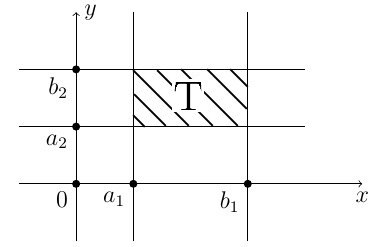
\includegraphics[scale=0.7]{img/633.jpg}
	\end{center}
  \item $n = 3 \Rightarrow \text{T} = \{ (x,y,z) \in \mathbb{R}^3 | a_1 \leqslant x \leqslant b_1, a_2 \leqslant y \leqslant b_2, a_3 \leqslant z \leqslant b_3  \}$ - прямоугольный параллелепипед T = $[a_1,b_1] \times [a_2,b_2] \times [a_3,b_3]$ \\
	$\mes \text{T} = (b_1-a_1)(b_2-a_2)(b_3-a_3)$ - объём данного прямоугольного параллелепипеда.
	\begin{center}
		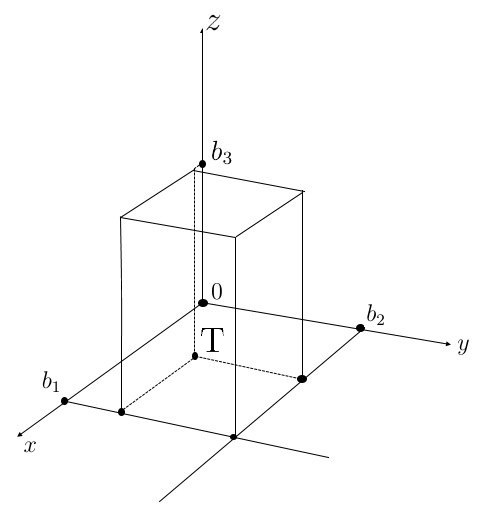
\includegraphics[scale=0.6]{img/634.jpg}
	\end{center}
\end{enumerate}

\important{Многогранником} $H \subset \RN$ будем называть произвольное конечное объединение параллелепипедов в $\RN$.

Если этот многогранник разбит на конечное число  составляющих параллелепипедов $\text{T}_k, k = \linebreak = \overline{1,m}$, у каждого из которых общими могут быть лишь граничные точки, т.е. $H = \bigcup\limits_{k=1}^m \text{П}_k$, то в этом случае полагают:
\begin{equation}
	\label{612}
	\mes H = \sum\limits_{k=1}^{m} \mes \text{T}_k.
\end{equation}
В дальнейшем считаем, что для пустого множества $\mes \emptyset = 0$.

Можно показать, что \eqref{612} не зависит от способа разбиения H на составляющие его параллелепипеды.

Для произвольного $D \subset \RN$ многогранник H считается \important{вписанным} в $D$, если $H \subset D$, и многогранник S считается  \important{описанным} около $D$, если $D \subset S$.

Величины
\begin{equation}
	\label{613}
	\begin{cases}
		m_* = \underset{\forall H \subset D}{\sup} \{ \mes H \}, \\
		m^* = \underset{\forall S \supset D}{\inf} \{ \mes S \},
	\end{cases}
\end{equation}
называются соответственно \important{нижней мерой} для D и \important{верхней мерой} для D.

По теореме о гранях, эти меры существуют (конечные или бесконечные).

В случае, когда $ m^* = m_{*} \in \mathbb{R} $,
множество $ D $ называется  \important{измеримым по Жордану} в пространстве $\RN$ и за его меру принимается $\mes D = m^* = m_{*}$.

Необходимым условием существования конечной меры (измеримости) по Жордану является ограниченность рассматриваемого множества $D \subset \RN$. В дальнейшем множество $D_0 \subset \RN$ будем называть \important{множеством меры нуль}, если для $\forall\; \varepsilon > 0 \;\;\; \exists\; H_\varepsilon \subset D_0$ и $\exists S_\varepsilon \supset D_0$, такие, что

\begin{equation}
	\label{614}
	\mes S_\varepsilon - \mes H_\varepsilon \leqslant \varepsilon,
\end{equation}
где $S_\varepsilon, H_\varepsilon$ - соответствующие многогранники в $\RN$.
\newpage
Для множеств меры нуль имеем следующие \important{свойства}:
\begin{enumerate}
  \item Пустое множество, одноточечное множество и множество, состоящее из конечного числа точек в $\RN$, является множеством меры нуль.
  \item Объединение конечного или счётного числа множеств меры нуль в $\RN$ будем множеством меры нуль.
  \item Любое подмножество множества меры нуль имеет нулевую меру.
\end{enumerate}
Критерием измеримости множества $D \subset \RN$ является его ограниченность и условие, что мера границы равна нулю ($ \mes \partial D = 0 $).

В общем случае для $\forall D_1, D_2 \subset \RN$ (любых измеримых) имеем:
\begin{equation}
	\label{615}
	mes (D_1 \cup D_2) = \mes D_1 + \mes D_2 - \mes(D_1 \cap D_2).
\end{equation}
Если в \eqref{615} мера пересечения $\mes(D_1 \cap D_2) = 0$, то имеем:
\begin{equation*}
    \mes (D_1 \cup D_2) = \mes D_1 + \mes D_2,
\end{equation*}
что выражает свойство конечной аддитивности меры Жордана в $\RN$.

Аналогично, если мера $\mes(D_i \cap D_j) = 0, \forall i \ne j, i = \overline{1,m}, j = \overline{1,m}$, то методом математической индукции (ММИ) доказывается, что
\begin{equation}
	\label{616}
	\mes \left(\bigcup_{k=1}^m D_k \right) = \sum_{k=1}^{m} \mes D_k.
\end{equation}

Равенство \eqref{616} заведомо выполняется для измеримых множеств в $D_k \in \RN, k = \overline{1,m}$ в случае, когда у них общими могут быть лишь граничные точки.

\subsection{Интегральные суммы и интеграл ФНП}

Для измеримого множества $D \subset \RN$ рассмотрим произвольное разбиение ${\forall P = \set{P_k}}$, ${k = \overline{1, m}}$, где $\forall P_k \subset D$ измеримы в $D$, и они имеют между собой
общими лишь может быть только граничные точки. В этом случае:
\begin{equation*}
	D = \bigcup\limits_{k = 1}^m P_k\; \text{ и } \mes(P_i \cap P_j) = 0, i \neq j; i, j = \overline{1, m}.
\end{equation*}

Выбирая произвольным образом отмеченное множество точек $Q = \set{M_k}, \forall M_k \in P_k, $
$k = \overline{1, m}$,
для ФНП $f(x)$, определённой для $\forall x \in D \subset \RN$ рассмотрим интегральную сумму:
\begin{equation}
	\label{eq:6.2-integral-sum}
	\sigma = \sigma(f, \{P; Q\}) = \sum\limits_{k = 1}^mf(M_k)\Delta{P_k},
\end{equation}
где $\Delta{P_k} = \mes P_k, k = \overline{1, m}$.

В дальнейшем величину $r_k = \max d(A; B)$, где $ \forall A, B \in P_k$, будем называть \important{диаметром}
множества $P_k \subset D$. Геометрически $r_k$ представляет собой диаметр $n$-мерного шара
наименьшего размера, содержащего $P_k$.

% Для краткости введём обозначение $r_k = \diam P_k, k = \overline{1, m}$.
Величину
${r = \max\set{r_k}}$, ${1 \leqslant k \leqslant m}$, будем называть \important{диаметром} используемого разбиения и
обозначать $r = \diam P$.

Функция $f(x)$, определённая для $x = (x_1, \ldots, x_n) \in D$, где $D \subset \RN$- измеримое
множество, считается интегрируемой на $D$, если
\begin{equation}
    \label{eq:6.2-integrity-definition}
	\exists I \subset \RN, \text{ что для }\forall \varepsilon > 0, \exists \delta > 0, \forall \set{P; Q},
	r = \diam P \leqslant \delta \Rightarrow \abs{I  - \delta}
	\overset{\eqref{eq:6.2-integral-sum}}{\leqslant} \varepsilon.
\end{equation}

Число $ I \in \mathbb{R} $ в \eqref{eq:6.2-integrity-definition}
будем называть значением $n$-кратного интеграла.
\begin{equation*}
	I = \underset{D}{\iint\ldots\int} f(x_1, \ldots, x_n) d x_1 \ldots dx_n = \int\limits_{D}f(x)dx
\end{equation*}

В дальнейшем будем также писать $I \overset{\eqref{eq:6.2-integral-sum}-
  \eqref{eq:6.2-integrity-definition}}{=}{\lim\limits_{r \to 0} \sigma}$.

При $n = 2$ для $ D \subset \mathbb{R}^2 $ интеграл \eqref{eq:6.2-integrity-definition} будем называть двойным (2И) и
обозначать в прямоугольной декартовой системе координат $Oxy$:
\begin{equation*}
\label{eq:6.2-double-integral}
I = \iint\limits_{D }f(x, y)dxdy,
\end{equation*}
а при $n = 3$ для $ D \subset \mathbb{R}^3 $ интеграл \eqref{eq:6.2-integrity-definition} будем называть тройным (3И) и обозначать в прямоугольной декартовой системе координат $Oxyz$:
\begin{equation*}
I = \iiint\limits_{D }f(x, y, z)dxdydz.
\end{equation*}

\begin{example}
	Пусть $f(x) \equiv 1, \forall x \in D \subset \RN$, где $D$ - измеримое множество. В этом
	случае
	\begin{equation*}
		\sigma 	\overset{\eqref{eq:6.2-integral-sum}}{=} \sum\limits_{k = 1}^m\Delta{P_k} =
		\sum_{k = 1}^m \mes P_k
	\end{equation*}
	поэтому в данном случае:
	\begin{equation}
		\label{eq:6.2-integral-example1}
        I = \lim\limits_{r \to 0}\sigma = \lim\limits_{r \to 0}(\mes D) = \mes D, \text{ т.е. }
		\int\limits_D dx = \mes D.
	\end{equation}
\end{example}

Равенство \eqref{eq:6.2-integral-example1} выражает простейший геометрический смысл $n$-кратного интеграла.
\begin{itemize}
  \item В случае $n = 1$ \eqref{eq:6.2-integral-example1} соответствует длине используемого отрезка
	интегрирования \\${D = \interval[{a; b}] \subset \R{}}$ ${(\mes D = b - a)}$.
  \item В случае $n = 2$ \eqref{eq:6.2-integral-example1} выражает площадь из $D \subset \R{2}$ в прямоугольной декартовой системе координат $Oxy$:
	\begin{equation*}
		\mes D = \iint\limits_{D \subset \R{2}}dxdy = \text{Площадь } D.
	\end{equation*}
  \item В случае $n = 3$ для измеримого $D \subset \R{3}$ получаем объём в прямоугольной декартовой системе координат $Oxyz$:
	\begin{equation*}
		\mes D = \iiint\limits_{D \subset \R{3}}dxdydz = \text{Объём } D.
	\end{equation*}
\end{itemize}

Как и для однократного интеграла ($n = 1$), множество интегрируемых на $D \subset \RN$ функций будем обозначать
$\mathbb{R}(D)$. Имеем следующие основные свойства $n$-кратных интегралов:
\begin{enumerate}
  \item \important{Линейность}\\
	Если $f, g \in \mathbb{R}(D)$для измеримого $D \subset \RN$, то
	\begin{equation*}
		\begin{split}
			&\forall \lambda, \mu \in \mathbb{R} \Rightarrow (\lambda f + \mu g) \in \mathbb{R}(D),\text{ причём} \\
			&\int\limits_D (\lambda f(x) + \mu g(x))dx = \lambda \int\limits_D f(x)dx +
			\mu \int\limits_D g(x)dx.
		\end{split}
	\end{equation*}
  \item \important{Аддитивность}\\
	Если $f \subset \mathbb{R}(D), D = D_1 \bigcup D_2$, где $D_1$, $D_2$ - измеримые множества в $\RN$,
	общими у которых могут быть лишь только граничные точки (${ \mes(D_1 \cap D_2) = 0 }$), то:
	\begin{equation*}
		\int\limits_{D}fdx = \int\limits_{D_1}fdx + \int\limits_{D_2}fdx.
	\end{equation*}
  \item \important{Неотрицательность}\\
	Пусть $f \in \mathbb{R}(D)$ и
    $ \forall x \in D \subset \RN \Rightarrow f(x) \geqslant 0 $, где
	$D$ - измеримое множество в $\RN$. Тогда:
	\begin{equation*}
		\int\limits_Df(x)dx \geqslant 0.
	\end{equation*}
  \item \important{Монотонность}\\
	Если $f, g \in \mathbb{R}(D)$ и $\forall x \in D \subset \RN \Rightarrow f(x) \leqslant g(x)$,
	где $D$ - измеримое множество в $\RN$, то:
	\begin{equation*}
		\int\limits_Df(x)dx \leqslant \int\limits_Dg(x)dx.
	\end{equation*}
  \item \important{Основная оценка}\\
	Пусть $\forall x \in D \subset \RN \Rightarrow m_0 \leqslant f(x) \leqslant M_0$, где
	$m_0, M_0 \in \mathbb{R}$, а $D$ - измеримое множество в $\RN$. Тогда:
	\begin{equation*}
		m_0 \mes D \leqslant \int\limits_D f(x) dx \leqslant M_0 \mes D.
	\end{equation*}
\end{enumerate}

Обоснование всех этих свойств проводится по той же схеме, что и для однократного интеграла.

Аналогично Ф1П обосновываются критерий Гейне и критерий Коши интегрируемости ФНП,
а также $C$-лемма для критерия Коши интегрируемости ФНП. На основании этого, так же, как и для
однократных интегралов, доказывается
\begin{theorem}[об интегрируемости непрерывных ФНП]
    $  $

	Если $f \in C(D)$, т.е. непрерывна на измеримом компакте $D \subset \RN$, то $f \in \mathbb{R}(D)$,
	т.е. интегрируема на $D$.
\end{theorem}

\newpage
\begin{consequence}[теорема о среднем для ФНП]

	Пусть $f \in C(D)$, а $g \subset \mathbb{R}(D)$, где $D \subset \RN$ - измеримый компакт. Если
	$\forall x \in D $ функция $g(x)$ сохраняет один и тот же знак, то $\exists x_0 \in D \subset \RN \Rightarrow$
	\begin{equation}
		\label{eq:6.2-intermediate-value}
        % \Rightarrow
		\int\limits_D f(x)g(x)dx =
		f(x_0)\int\limits_Dg(x)dx.
	\end{equation}
	Доказательство по той же схеме, что и для Ф1П.
\end{consequence}

\begin{note}
	Если взять в \eqref{eq:6.2-intermediate-value} $g(x) \equiv 1, \forall x \in D$, то, учитывая
	предыдущий пример, получаем:
	\begin{equation*}
		\text{если } f \in C(D), \text{ то }\exists x_0 \in D \text{ такое, что } \int\limits_Df(x)dx = f(x_0) \mes D,
	\end{equation*}
	что соответствует простейшей теореме о среднем для непрерывной, а значит, интегрируемой, ФНП.
\end{note}

\subsection{Двойной интеграл (2И)}

Рассмотрим функцию $f(x,y), \forall (x,y) \in D \subset \mathbb{R}^2$, где $D$ - измеримое множество в $\mathbb{R}^2$, т.е. плоская квадрируемая фигура. В этом случае имеем 2И:
\begin{equation}
	\label{eq:6.2-11}
	I = \iint\limits_{D} f(x,y)dxdy.
\end{equation}
\begin{theorem}[о вычислении 2И по прямоугольнику для непрерывных Ф2П]
	Пусть $f(x)$ непрерывна на прямоугольнике: П $= [a;b]\times[c;d] = \defineset{(x,y) \in \mathbb{R}^2 }{a \leq x \leq b, c \leq y \leq d}$.

	Тогда для \eqref{eq:6.2-11} следует:
	\begin{equation}
		\label{eq:6.2-12}
		I = \int\limits_{a}^b \left(\int\limits_{c}^d f(x,y)dy\right)dx =  \int\limits_{c}^d \left(\int\limits_{a}^b f(x,y)dx\right)dy.
	\end{equation}
\end{theorem}
\begin{proof}
	Рассмотрим произвольное разбиение: $\widetilde{P} = \{ x_i \}, i = \overline{1,m}$ отрезка $[a;b]: $\\ $a = x_0 < x_1 < \ldots < x_{i-1} < x_i < x_{i+1} < \ldots < x_m = b$ и произвольное разбиение: $\bar{P} = \{y_j\}, j = \overline{1,l}$ отрезка $[c;d]: c = y_0 < y_1 < \ldots < y_{j-1} < y_j < y_{j+1} < \ldots < y_l = d$.

	С помощью вертикальных прямых $x = x_i, i = \overline{1, m}$ и горизонтальных прямых $y = y_j,$ \\$ j = \overline{1, l}$ прямоугольник П $= [a;b]\times[c;d]$ разобьётся на части $ \text{П}_{i,j}= [x_{i-1};x_i]\times[y_{j-1};y_j]$, образующие соответствующее разбиение П = $\bigcup\limits_{i = 1}^m \bigcup\limits_{j = 1}^l \text{П}_{i,j}$ на  составляющие его прямоугольника $\text{П}_{i,j}$, у которых общими могут быть лишь граничные точки.

	\begin{center}
		\begin{tikzpicture}
			\coordinate (left) at (-1.0, 0.0);
			\coordinate (right) at (5.0, 0.0);
			\coordinate (top) at (0.0, 3);
			\coordinate (bottom) at (0.0, -1.0);
			\coordinate (center) at (0.0, 0.0);
			\draw[->] (left) -- (right);
			\draw[->] (bottom) -- (top);
			\draw (right) node[anchor=north] {$x$};
			\draw (top) node[anchor=west] {$y$};
			% \fill [black] (1.5, 1.5) circle (20pt);
			% \fill [white] (1.5, 1.5) circle (19pt);
			% Bottom part of plot
			% \draw[black, dashed] (1.5,1.5) circle (19pt);
			% \draw (1.5,1.5) circle (19pt);
			\draw[fill=black] (-0.5, -0.5) -- (3.0, -0.5);
			\draw[fill=black] (-0.5, -0.5) -- (-0.5, 2);
			\draw[fill=black] (3.0, 2.0) -- (-0.5, 2);
			\draw[fill=black] (3.0, 2.0) -- (3.0, -0.5);

			\draw[fill=black, dashed] (3.0, 1.2) -- (-0.5, 1.2);
			\draw (-0.5, 1.2) node[anchor=north east] {$y_{j-1}$};
			\fill [black] (-0.5, 1.2) circle (2pt);
			\draw (-0.5, 1.5) node[anchor=south east] {$y_{j}$};
			\fill [black] (-0.5, 1.5) circle (2pt);
			\draw[fill=black, dashed] (3.0, 1.5) -- (-0.5, 1.5);

			\draw (0.5, -0.5) node[anchor=north] {$x_{i-1}$};
			\fill [black] (0.5, -0.5) circle (2pt);
			\draw[fill=black, dashed] (0.5, -0.5) -- (0.5, 2);
			\draw (0.8, -0.5) node[anchor=north west] {$x_{i}$};
			\fill [black] (0.8, -0.5) circle (2pt);
			\draw[fill=black, dashed] (0.8, -0.5) -- (0.8, 2);
			\draw (0,-0.5) node[anchor=north east] {$c$};
			\fill [black] (0,-0.5) circle (2pt);
			\draw (0,2) node[anchor=south west] {$d$};
			\fill [black] (0,2) circle (2pt);
			\draw (-0.5,0) node[anchor=north east] {$a$};
			\fill [black] (-0.5,0) circle (2pt);
			\draw (3,0) node[anchor=north west] {$b$};
			\fill [black] (3,0) circle (2pt);
			
			\draw (0.8,2.1) node[anchor=north west] {$\text{П}_{i,j}$};
			\draw[fill=black] (0.8, 1.2) -- (0.5, 1.5);
			\draw[fill=black] (0.8, 1.3) -- (0.6, 1.5);
			\draw[fill=black] (0.8, 1.4) -- (0.7, 1.5);
			\draw[fill=black] (0.7, 1.2) -- (0.5, 1.4);
			\draw[fill=black] (0.6, 1.2) -- (0.5, 1.3);
			% \fill [black] (1.5,1.5) circle (2pt);
			% \fill [black] (1.5,0) circle (2pt);
			% \fill [black] (0, 1.5) circle (2pt);
			% \draw (1.37,1.37) node[anchor=south west] {$\boldsymbol{M_0}$};
			% \draw (1.5,-0.06) node[anchor=north] {$a$};
			% \draw (-0.06, 1.5) node[anchor=east] {$b$};
		\end{tikzpicture}
	\end{center}

	Так как $f \in C(\text{П}) $, то $ f \in C(\text{П}_{i,j}), \forall i = \overline{1,m}, \forall j = \overline{1,l}$.

	Рассмотрим функцию $F_i(y) = \dint\limits_{x_{i-1}}^{x_i} f(x,y)dx, i = \overline{1,m}$.

    Этот интеграл существует, т.к. $\forall \fix y \Rightarrow f(x,y)$ - непрерывна по x. По теореме о среднем для однократных интегралов получаем, что:\\
	$\exists t_{i,j} \in [x_{i-1}; x_i] \Rightarrow F_i(y_j) = \dint\limits_{x_{i-1}}^{x_i} f(x,y_j)dx = f(t_{i,j}, y_j) \Delta x_i$, где $\Delta x_i = x_i - x_{i-1}, i = \overline{1,m}$.

	В соответствии с этим определены точки $M_{i,j} = (t_{i,j}, y_j) \in \text{П}_{i,j}$.

	Таким образом, для прямоугольника П имеем разбиение $P = \{ \text{П}_{i,j} \} $ с множеством отмеченных точек $Q = \{M_{i,j} \}$. Для получаемой специальной интегральной суммы
	\begin{equation}
		\label{eq:6.2-13}
		\sigma = \sigma \left(f; \{P; Q\}\right) = \sum\limits_{i=1}^{m} \sum\limits_{j=1}^{l} f\left(M_{i,j}\right) \Delta \text{П}_{i,j},
	\end{equation}
	где $\Delta \text{П}_{i,j}$ = площадь $\text{П}_{i,j} = (x_i - x_{i-1})(y_j - y_{j-1}) = \Delta x_i \Delta y_j:$
	\begin{equation*}
		\begin{cases}
			\Delta x_i = x_i - x_{i-1}, i = \overline{1,m}, \\
			\Delta y_j = y_j - y_{j-1}, j = \overline{1,l},
		\end{cases}
	\end{equation*}
	имеем $\displaystyle \sigma = \sum\limits_{j=1}^{l} \sum\limits_{i=1}^{m} f(M_{i,j}) \Delta x_i \Delta y_j = \sum\limits_{j=1}^{l} \sum\limits_{i=1}^{m} F_i(y_j) \Delta y_j = \sum\limits_{j=1}^{l} \sum\limits_{i=1}^{m} \left(\nullFrac\dint\limits_{x_{i-1}}^{x_i} f(x,y_j) dx\right) \Delta y_j = \\
	= \begin{sqcases}\sum\limits_{i=1}^{m} \dint\limits_{x_{i-1}}^{x_i} f(x,y) dx = \dint\limits_{x_{1}}^{x_2} + \dint\limits_{x_2}^{x_3} + \ldots + \dint\limits_{x_{n-1}}^{x_n} = \dint\limits_{x_{1}}^{x_n} f(x,y)dx = \dint\limits_{a}^{b} f(x,y)dx   \end{sqcases} = $
	\begin{equation}
		\label{eq:6.3-14}
		= \sum\limits_{j=1}^{l} \left( \dint  \limits_{a}^{b}  f(x, y_j) dx \right) \Delta y_j
		=\sum\limits_{j=1}^{l} F(y_j) \Delta y_j,
	\end{equation}
	где
	\begin{equation}
		\label{eq:6.3-15}
		\begin{cases}
			F(y) = \dint\limits_{a}^{b} f(x,y) dx, \\
			y \in [a; b].
		\end{cases}
	\end{equation}
	Из \eqref{eq:6.3-14} следует, что $\sigma$ является одной из интегральных сумм для \eqref{eq:6.3-15}, вычисляемых на разбиении $\bar{P} = \{y_j\}, j = \overline{1, l}$. Отсюда при $\bar{r} = diam \bar{P} = \underset{1 \leqslant j \leqslant l}{max}\{\Delta y_j\} \to 0$, в силу непрерывности используемых функций следует:
	${\exists \dint\limits_c^d F(y)dy = \lim\limits_{\bar{r} \to 0} \sum\limits_{j=1}^{l} F(y_j) \Delta y_j = [\eqref{eq:6.3-14}] = \lim\limits_{\bar{r} \to 0} \sigma = I}$.

	В силу того, что из непрерывности функций следует их интегрируемость, а значит, возможность использования для вычисления $I$ не общих интегральных сумм, а специальных, получаем, что:
    % \begin{equation*}
    $
	I =  \dint\limits_{c}^{d} F(y) dy \overset{\eqref{eq:6.3-15}}{=} \dint\limits_c^d \left(\dint\limits_a^b f(x,y)dx \right) dy.
    $
    % \end{equation*}

	Аналогично доказывается и второе равенство \eqref{eq:6.2-12}.
\end{proof}

\newpage

\begin{notes}
  \item На практике формулы \eqref{eq:6.2-12} записываются в виде:
	$ I = \dint\limits_a^b dx \dint\limits_c^d f(x, y)dy = \dint\limits_c^d dy \dint\limits_a^b f(x,y) dx$.

	Такое представление 2И называется \important{представлением через повторные интегралы}.
  \item По аналогичной схеме доказывается, что
	\begin{itemize}
	  \item Если $f \in \mathbb{R}(\text{П})$ и $F \in \mathbb{R}[c;d]$, то:
		\begin{equation}
			\label{eq:6.3-16}
			I = \iint\limits_{\substack{a \leqslant x \leqslant b,\\ c \leqslant y \leqslant d}}
			f(x,y)dxdy = \dint\limits_c^d dy \dint\limits_a^b f(x,y) dx.
		\end{equation}
	  \item В случае, когда $f \in \mathbb{R}$(П) и функция \eqref{eq:6.3-17}
		\begin{equation}
			\label{eq:6.3-17}
			G(x) = \dint\limits_c^d f(x,y)dy
		\end{equation}
		интегрируема на $[a;b]$, получаем, что:
		\begin{equation}
			\label{eq:6.3-18}
			\iint\limits_{\substack{a \leqslant x \leqslant b, \\ c \leqslant y \leqslant d}}
			f(x,y)dxdy = \dint\limits_a^b G(x)dx = \dint\limits_a^b dx \dint\limits_c^d f(x,y)dy.
		\end{equation}
	\end{itemize}
\end{notes}

\begin{consequence}[о вычислении 2И по криволинейной трапеции]
\end{consequence}

Если $f \in C(\widetilde{T})$, где $\widetilde{T}$ - криволинейная трапеция вдоль оси Oy, т.е.
\begin{equation}
	\label{eq:6.3-19}
	\widetilde{T} = \{(x,y)\in\mathbb{R}^2 | c(x) \leqslant y \leqslant d(x), a \leqslant x \leqslant b\},
\end{equation}
то в случае, когда $ c(x) $ и $ d(x) $ непрерывны на [a;b], имеем:
\begin{equation}
	\label{eq:6.3-20}
	\iint\limits_{\substack{a \leqslant x \leqslant b, \\ c(x) \leqslant y \leqslant d(x)}}
	f(x,y)dxdy = \dint\limits_a^b dx \dint\limits_{c(x)}^{d(x)} f(x,y)dy.
\end{equation}
Аналогично, если $f \in C(\bar{T})$, где $\bar{T}$ - криволинейная трапеция вдоль оси $ Ox $, т.е.:
\begin{equation}
	\label{eq:6.3-21}
	\bar{T} = \{(x,y)\in\mathbb{R}^2 | a(y) \leqslant x \leqslant b(y), c \leqslant y \leqslant d \},
\end{equation}

то в случае, когда $a(y), b(y)$ - непрерывны на $[c,d]$, получаем:
\begin{equation}
	\label{eq:6.3-22}
	\iint\limits_{\substack{c \leqslant y \leqslant d, \\ a(y) \leqslant x \leqslant b(y)}}
	f(x,y)dxdy = \dint\limits_c^d dy \dint\limits_{a(y)}^{b(y)} f(x,y)dx.
\end{equation}
\begin{proof}
	В случае трапеции \eqref{eq:6.3-19} рассмотрим функцию
	\begin{equation*}
		f_0(x,y) = \begin{cases}
			f(x,y), (x,y) \in \widetilde{T}, \\
			0, (x,y) \notin \widetilde{T}.
		\end{cases}
	\end{equation*}
	Для непрерывных на $[a;b]$ функций $ c(x) $ и $ d(x) $ из теоремы Вейерштрасса следует:
	\begin{equation*}
		\begin{cases}
			\exists c_0 = \min \; c(x) \in \mathbb{R}, x \in [a;b], \\
			\exists d_0 = \max \; d(x) \in \mathbb{R}, x \in [a;b].
		\end{cases}
	\end{equation*}
	\begin{center}
		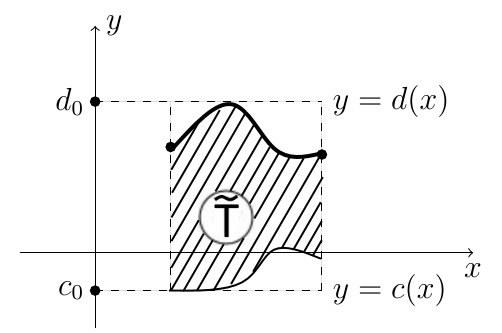
\includegraphics[scale=0.6]{img/631.jpg}
	\end{center}
	Отсюда, используя прямоугольник $\text{П}_0 = [a;b] \times [c_0;d_0]$, в силу аддитивности ОИ и 2И имеем:
	$\displaystyle
    \iint\limits_{\widetilde{T}} f(x,y)dxdy = \iint\limits_{\widetilde{T}} f(x,y)dxdy + \iint\limits_{\text{П}_0 \setminus \widetilde{T}} 0 dxdy = \iint\limits_{\widetilde{T}} f(x,y)dxdy + \iint\limits_{\text{П}_0 \setminus \widetilde{T}} f_0(x,y) dxdy =
    $
    \\
    $
    \displaystyle
    = \iint\limits_{\text{П}_0} f_0(x,y) dxdy = [\eqref{eq:6.3-18}] = \dint\limits_{a}^b dx \dint\limits_{c_0}^{d_0} f_0(x,y) dy =$ \\
	$= \begin{sqcases} \dint\limits_{c_0}^{d_0} f_0(x,y)dy = \dint\limits_{c_0}^{c(x)} f_0(x,y)dx + \dint\limits_{c(x)}^{d(x)} f_0(x,y)dx + \dint\limits_{d(x)}^{d_0} f_0(x,y)dx = \dint\limits_{c(x)}^{d(x)} f_0(x,y)dx \end{sqcases} = $\\
    $= \dint\limits_{a}^{b} dx \dint\limits_{c(x)}^{d(x)}f_0(x, y)dy dy$
	$= \dint\limits_{a}^{b} dx \dint\limits_{c(x)}^{d(x)} f(x,y)dy$.

	Аналогично в случае трапеции \eqref{eq:6.3-21} обосновывается формула \eqref{eq:6.3-22}.
\end{proof}
\newpage

\begin{example}
	Рассмотрим $\displaystyle I = \iint\limits_{x^2 + y^2 \leqslant 2x} f(x,y)dxdy$.

	Для области интегрирования $ T $ следует:
	$x^2 + 2x + y^2 \leqslant 0 \Rightarrow (x-1)^2 + y^2 \leqslant 1$, т.е. $T$ - круг с центром в точке C(1,0) и радиуса $R = 1$.

	\begin{enumerate}
	  \item Если $x \in [0;2]$, то из неравенства $y^2 \leqslant 2x - x^2 \Rightarrow -\sqrt{2x - x^2} \leqslant y \leqslant \sqrt{2x - x^2}$.

		\begin{center}
			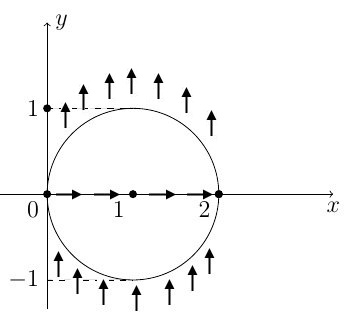
\includegraphics[scale=0.7]{img/632.jpg}
		\end{center}
		В данном случае круг $ T $ можно рассматривать как криволинейную трапецию вдоль оси $ Oy $. Здесь для определения изменения $ x $ следует спроектировать $ T $ на ось $ Ox $ и \important{двигаться по оси $ Ox $}. В результате получаем: $0 \leqslant x \leqslant 2$.

		Для определения линий входа и выхода при движении \important{вдоль оси $ Oy $} имеем:
		\\
		$y = - \sqrt{2x - x^2}$ - линия входа в $ T $, $y =  \sqrt{2x - x^2}$ - линия выхода из $ T $.

		Отсюда в силу \eqref{eq:6.3-20} следует:
		\begin{equation*}
			I = \dint\limits_0^2 dx \dint\limits_{- \sqrt{2x - x^2}}^{\sqrt{2x - x^2}} f(x,y)dy.
		\end{equation*}
	  \item Будем рассматривать наш круг T как криволинейную трапецию вдоль оси $ Ox $, в этом случае проектирование $ T $ на $ Oy $ даёт $ -1 \leqslant y \leqslant 1 $, а при решении уравнения \\
        $(x-1)^2 \leqslant 1-y^2$ получаем:
		$1 - \sqrt{1-y^2} \leqslant x \leqslant 1 + \sqrt{1-y^2}$, \\
        т.е. при движении \important{вдоль оси $ Ox $} имеем:
        \\
		$x = 1 - \sqrt{1 - y^2}$ - линия входа в $ T $, $x = 1 + \sqrt{1 - y^2}$ - линия выхода из $ T $.

		Отсюда в силу \eqref{eq:6.3-22} следует: $I = \dint\limits_{-1}^1 dy \dint\limits_{1 - \sqrt{1 - y^2}}^{1 + \sqrt{1 - y^2}} f(x,y)dx$.
	\end{enumerate}
	Отметим, что на практике для представления 2И через повторные интегралы, в случае более сложных областей интегрирования
	при возможности разбивают используемую область вертикальными и горизонтальными прямыми на соответствующие криволинейные трапеции либо вдоль $ Ox $, либо вдоль $ Oy $.
	Если таких трапеций конечное число, то используют аддитивность 2И и рассматривают пределы интегрирования для каждой трапеции в отдельности.
\end{example}

\subsection{Тройной интеграл}
Рассмотрим $f(x, y, z)$, определённую в $\forall (x, y, z) \in H \subset \R{3}$, где $H$ - измеримое
множество в $\R{3}$, т.е. некоторое кубируемое тело. В данном случае имеем тройной интеграл
\begin{equation}
	\label{eq:6.4-triple-integral}
	I = \iiint\limits_H f(x, y, z)dxdydz.
\end{equation}

\begin{theorem}[о сведении вычисления 3И к 2И]
    Пусть $H$ - цилиндрическое тело вдоль оси $Oz$, т.е:
    \begin{equation}
		\label{eq:6.4-symmetric-body}
		H = \defineset{(x, y, z) \in \R{3}}{(x, y) \in D \subset \R{2}, p \leqslant z \leqslant q},
    \end{equation}
    где $p, q \in \R{}$, а $D$ - квадрируемый компакт в $\R{2}$.

    Если $f \in C(H)$, т.е. непрерывна на $H$, то
    \begin{equation}
		\label{eq:6.4-triple-to-double-integral}
		I \overset{\eqref{eq:6.4-triple-integral}}{=} \iint\limits_D
		\parenthesis{\int\limits_p^q f(x, y, z)dz}dxdy.
    \end{equation}
\end{theorem}

\begin{proof}
    проводится по той же схеме, что и при вычислении 2И по прямоугольнику. Вначале рассматриваем произвольное
    разбиение ${\forall P_0 = \set{z_k}, k = \overline{0, m}}$, отрезка $\interval[{p; q}]$ на части
    ${p = z_0 < z_1 < \ldots < z_{m - 1} < z_m = q}$. В соответствии с этим разбиением, в силу
    непрерывности $f$ на $H$, имеем непрерывную Ф2П:
    \begin{equation}
		\label{eq:6.4-proof-theorem1-e1}
		F(x, y) = \int\limits_p^q f(x, y, z)dz, k = \overline{1, m}.
    \end{equation}
    Далее, проводя произвольное разбиение $\forall \widetilde{P_0}$ квадрируемого компакта
    $D \subset \R{2}$,
    являющегося проекцией $H \subset \R{3}$, на $Oxy$, имеем:
    \begin{center}
        ${T_0 = \set{D_j}, j = \overline{1, l}}$,
        где $\bigcup\limits_{j = 1}^lD_j = D$ и $\mes(D_j \cap D_i) = 0$, ${i \neq j}$.
    \end{center}

    Выбирая произвольным образом множество отмеченных точек:
    \begin{equation*}
		\widetilde{Q_0} = \set{M_j}, \forall M_j = (x_j, y_j) \in D_j, j = \overline{1, l},
    \end{equation*}
    Рассмотрим
    \begin{equation}
		\label{eq:6.4-proof-theorem1-e2}
		I_{kj} = \int\limits_{z_{k - 1}}^{z_k}f(x_j, y_j, z) dz.
    \end{equation}
		По теореме о среднем получаем, что $
        \exists t_{kj} \in \interval[{z_{k - 1}; z_k}] \Rightarrow
		I_{kj} = f(x_j, y_j, t_{kj})(z_k - z_{k-1}) = \linebreak = f(N_{kj})\Delta{z_k}$,
    \begin{equation}
	    \label{eq:6.4-proof-theorem1-e3}
        \text{где }
		\begin{cases}
			N_{kj} = (x_j, y_j, t_{kj}) = (M_j, t_{kj})\\
			\Delta{z_k} = z_k - z_{k - 1}\\
			k = \overline{1, m}, j = \overline{1, l}\\
		\end{cases}
    \end{equation}

    Отсюда при $r_0 = \diam{\widetilde{P_0}} \to 0$ имеем
    \begin{equation}
		\label{eq:6.4-proof-theorem1-e4}
		I_0 = \iint\limits_D F(x, y) dxdy = \lim\limits_{r_0 \to 0}\widetilde{\sigma_0}, \text{ где }
    \end{equation}
    \begin{equation*}
		\begin{split}
			&\widetilde{\sigma_0} = \sigma(F_i(\widetilde{P_0}, \widetilde{Q_0})) =
			\sum\limits_{j = 1}^l F(M_j) \mes D_j = \begin{sqcases}F
				\overset{\eqref{eq:6.4-proof-theorem1-e1}}{=} \dint_p^q fdz = \dint_{z_0=p}^{z_1} + \ldots
				+ \dint_{z_{m - 1}}^{z_m=q} = \sum\limits_{k = 1}^m\dint_{z_{k - 1}}^{z_k}fdz\end{sqcases}=\\
			&=\sum\limits_{j = 1}^l(\sum\limits_{k = 1}^m\dint_{z_{k - 1}}^{z_k} f(M_j, z)dz) \mes D_j
			\overset{\eqref{eq:6.4-proof-theorem1-e2}}{=} \sum\limits_{j = 1}^l\sum\limits_{k = 1}^m
			I_{kj}\mes D_j =
		\end{split}
    \end{equation*}
    \begin{equation}
		\label{eq:6.4-proof-theorem1-e5}
		=\sum\limits_{j = 1}^l\sum\limits_{k = 1}^mf(N_{kj})\Delta{z_k}\mes{D_j}.
    \end{equation}

    Эту сумму \eqref{eq:6.4-proof-theorem1-e5} можно рассматривать как специальную интегральную
    сумму $\sigma_0$ для \eqref{eq:6.4-triple-to-double-integral}, построенную по разбиению
    ${P = (H_{kj})}$ с множеством отмеченных точек
    % $N = (x_j, y_j, t_{kj})$,
    ${Q = \set{N_{kj}}}$, где
    $H_{kj} = D_j \times [{z_{k - 1},  z_k}]$, ${N_{kj} = (x_j, y_j, t_{kj}) \in H_{kj},	  k = \overline{1, m}, j = \overline{1, l}}$. Действительно:
    \begin{equation*}
		\sigma_0 = \sigma_0(f; \set{P, Q}) = \sum\limits_{k = 1}^m\sum\limits_{j = 1}^lf(N_{kj})\mes H_{kj} =
		\begin{sqcases}
			\mes H_{kj} = \text{объём}(D_j \times \interval[{z_{k - 1}; z_k}]) =\\
			=(\text{площадь }D_j)(z_k - z_{k - 1}) = \mes D_j \Delta{z_k}
		\end{sqcases}=
    \end{equation*}
    \begin{equation}
		\label{eq:6.4-proof-theorem1-e6}
		=\sum\limits_{k = 1}^m\sum\limits_{j = 1}^lf(N_{kj})\mes D_j \Delta{z_k}
		\overset{\eqref{eq:6.4-proof-theorem1-e5}}{=} \widetilde{\sigma_0}.
    \end{equation}
    Поэтому, учитывая, что при ${r = \diam P \to 0 \Rightarrow r_0 = \diam \widetilde{P_0} \to 0}$,
    в силу непрерывности $f(x, y, z)$ на компакте $H \subset \R{3}$ имеем:
    \begin{equation*}
		\begin{split}
			&I \overset{\eqref{eq:6.4-proof-theorem1-e1}}{=}
			\lim\limits_{r \to 0}\sigma_0\overset{\eqref{eq:6.4-proof-theorem1-e6}}{=}
			\lim\limits_{r_0 \to 0}\widetilde{\sigma_0 }\overset{\eqref{eq:6.4-proof-theorem1-e4}}{=}
			\iint\limits_D F(x, y)dxdy \overset{\eqref{eq:6.4-symmetric-body}}{=} \iint\limits_D
			\parenthesis{\int\limits_p^q f(x, y, z)dz}dxdy = \\
			&=\iint\limits_D dxdy\int\limits_p^qf(x, y, z)dz
		\end{split}
    \end{equation*}
\end{proof}

\begin{notes}
  \item Если компакт $H \subset \R{3}$ является цилиндроидом вдоль оси $Oz$, т.е:
    \begin{equation*}
		H = \defineset{(x, y, z) \in \R{3}}{p(x, y) \leqslant z \leqslant q(x, y), (x, y) \in D},
    \end{equation*}
    $p(x, y), q(x, y)$ - непрерывные на квадрируемом компакте $D \subset \mathbb{R}^2$, то для $f \in C(H)$:
    \begin{equation}
		\label{eq:6.4-note1}
		I \overset{\eqref{eq:6.4-triple-to-double-integral}}{=} \iint\limits_D \left( \nullFrac\int\limits_{p(x, y)}^{q(x, y)}
		  f(x, y, z) dz \right) dxdy.
    \end{equation}
    $ {
	  \text{
		Обоснование \eqref{eq:6.4-note1} проводится по той же схеме, что и в соответствующем случае для 2И.
	  }
	} $

  \item Если компакт $H \subset \R{3}$ является цилиндроидом \eqref{eq:6.4-note1} вдоль оси $Oz$, где квадрируемый компакт $D \subset \R{2}$ является некоторой
    криволинейной трапецией вдоль оси $Oy$ и, значит,
    \begin{equation*}
		H = \defineset{(x, y, z) \in \R{3}}{p(x, y) \leqslant z \leqslant q(x, y),
		  c(x) \leqslant y \leqslant d(x), a \leqslant x \leqslant b},
    \end{equation*}
    то в случае непрерывности используемых функций получаемое представление для 3И через
    повторные интегралы:
    \begin{equation}
		\label{eq:6.4-note2}
		I \overset{\eqref{eq:6.4-triple-to-double-integral}}{=}
		\int\limits_a^bdx\int\limits_{c(x)}^{d(x)}dy\int_{p(x, y)}^{q(x, y)}f(x, y, z)dz.
    \end{equation}
  \item Формула \eqref{eq:6.4-note2} естественным образом обобщается на случаи соответствующих
    трапеций и цилиндроидов вдоль других координатных осей. В общем
    случае, когда компакт $H \subset \R{3}$ является объединением конечного числа таких цилиндроидов,
    вычисление \eqref{eq:6.4-triple-to-double-integral} в силу аддитивности 3И сводится к вычислению
    интегралов по элементарным цилиндроидам вдоль какой-либо из осей.
\end{notes}

\begin{example}
	Для непрерывной на $\interval[{0; 1}]$ функции $g(z)$ рассмотрим 3И, заданный в виде повторного
	интеграла:
	\begin{equation*}
		I_0 = \int\limits_{-1}^1dx\int\limits_{-\sqrt{1 - x^2}}^{\sqrt{1 - x^2}}\int\limits_{x^2+y^2}^1 g(z)dz.
	\end{equation*}
	В данном случае имеем:
	\begin{equation*}
		I_0 \overset{\eqref{eq:6.4-triple-to-double-integral}}{=}\iiint\limits_Hg(z)dxdydz,
	\end{equation*}
	где $H$ - компакт в $\R{3}$, ограниченный в пространстве параболоидом ${z = x^2 + y^2}$ и
	плоскостью $z = 1$, проекцией которого на $Oxy$ является круг $D: x^2 + y^2 \leqslant 1$:
\begin{center}
	  [IMAGE NOT FOUND]
		% \includegraphics[scale=0.7]{img/635.jpg}
\end{center}
	Рассматривая $H$ как соответствующий  элементарный цилиндроид вдоль $Oy$, имеем:
	\begin{equation*}
		H = \defineset{(x, y, z) \in \R{3}}{\sqrt{z - x^2} \leqslant y \leqslant \sqrt{z - x^2},
		  -\sqrt{z} \leqslant x \leqslant \sqrt{z}, 0 \leqslant z \leqslant 1}
	\end{equation*}
	Переходя в таком виде снова к повторному интегралу, получаем:
	\begin{equation*}
		\begin{split}
			&I_0 = \int\limits_0^1dz\int\limits_{-\sqrt{z}}^{\sqrt{z}}dx\int\limits_{-\sqrt{z - x^2}}^{\sqrt{z - x^2}}g(z)dy =
			\int\limits_0^1dz\int\limits_{-\sqrt{z}}^{\sqrt{z}} \begin{sqcases} yg(z) \end{sqcases}_{y = -\sqrt{z - x^2}}^{y = \sqrt{z - x^2}} dx =
			2\int\limits_0^1dz\int\limits_{-\sqrt{z}}^{\sqrt{z}}g(z)\sqrt{z - x^2}dx =\\
			&=\begin{sqcases}\dint\sqrt{a^2 - x^2}dx = \frac{x}{2}\sqrt{a^2 - x^2} + \frac{a^2}{2}\arcsin{\frac{x}{a}} + c\end{sqcases} =
			4\dint\limits_0^1g(z)
			\begin{sqcases}\frac{x}{2}\sqrt{z - x^2} + \frac{z}{2}\arcsin{\frac{x}{\sqrt{z}}}\end{sqcases}_{x = 0}^{x = \sqrt{z}}dz =\\
			&=4\int\limits_0^1g(z)\frac{\pi z}{4}dz = \pi\int\limits_0^1zg(z)dz.
		\end{split}
	\end{equation*}
	Изменив порядок интегрирования мы свели вычисление тройного интеграла к вычислению
	соответствующего однократного интеграла.
\end{example}

\subsection{Замена переменных в $n$-кратном интеграле}
Рассмотрим множества $D \subset \R{n}$ и $G \subset \R{n}$. Множество $D$ будем рассматривать в системе координат $O_{x_1,\ldots x_n}$,
а множество $G$ - в системе координат $O_{t_1,\ldots t_n}$.

Пусть имеется отображение
\begin{equation}
	\label{eq:lecture6-34}
	f : G \to D,
\end{equation}
при котором $\forall t = (t_1, \ldots t_n) \in G$ ставится в соответствие
единственное ${f(t) = (f_1(t), \ldots f_n(t)) \in D}$. Отображение \eqref{eq:lecture6-34}
будет взаимно-однозначным, если оно инъективно, т.е. различным точкам из $G$
будут соответствовать различные точечные образы в $D$.

В случае взаимной одозначности \eqref{eq:lecture6-34} существует единственное
обратное отображение
\begin{equation}
	\label{eq:lecture6-35}
	g : D \to G,
\end{equation}
при котором $\forall x \in D \exists ! t = g(x) \in G \suchthat f(t) = x$.

Если во взаимооднозначных соотношениях \eqref{eq:lecture6-34}, \eqref{eq:lecture6-35}
используется непрерывно дифференцируемая функция, то говорят, что множества $D$
и $G$ \important{диффеоморфны}, а отображения \eqref{eq:lecture6-34},
\eqref{eq:lecture6-35} - диффеоморфизмы.

Для диффеоморфизма \eqref{eq:lecture6-34} его Якобиан - это определитель
\begin{equation}
	\label{eq:lecture6-36}
	J(t) = \det\dfrac{\partial F}{\partial t} =
	\begin{vmatrix}
		\frac{\partial F_1}{\partial t_1} & \ldots & \frac{\partial F_1}{\partial t_n}\\
		\vdots & \ddots & \vdots\\
		\frac{\partial F_n}{\partial t_1} & \ldots & \frac{\partial F_n}{\partial t_n}\\
	\end{vmatrix}.
\end{equation}
Якобиан обратного диффеоморфного отображения \eqref{eq:lecture6-35} будем обозначать
\begin{equation}
	\label{eq:lecture6-37}
	\mathcal{J}(t) = \det\dfrac{\partial g}{\partial x} =
	\begin{vmatrix}
		\frac{\partial g_1}{\partial x_1} & \ldots & \frac{\partial g_1}{\partial x_n}\\
		\vdots & \ddots & \vdots\\
		\frac{\partial g_n}{\partial x_1} & \ldots & \frac{\partial g_n}{\partial x_n}\\
	\end{vmatrix}.
\end{equation}

Используя свойства определителя можно показать, что \eqref{eq:lecture6-36} и
\eqref{eq:lecture6-37} удовлетворяют условию $J(t) \mathcal{J}(t) = 1$, откуда, в
 частности, следует, что при диффеоморфизме \eqref{eq:lecture6-34} и \eqref{eq:lecture6-35} якобианы \eqref{eq:lecture6-36} и
\eqref{eq:lecture6-37} - ненулевые определители.

Можно показать, что диффеоморфизме \eqref{eq:lecture6-34} для меры $\mes  G$ образа и меры прообраза $\mes D$ имеем:
\begin{equation}
	\label{eq:measure-statement}
	\mes D = \int_G \abs{f(t)}dt = \underset{G}{\int \ldots \int}\abs{J(t_1, \ldots t_n)}dt_1 \ldots dt_n
\end{equation}
Обоснование \eqref{eq:measure-statement} для случая $n = 2$ и $n = 3$ будет сделано позже.

\begin{theorem}[о замене переменных в $ n $-кратном интеграле]$  $

    Если для диффеоморфизма \eqref{eq:lecture6-34} и для функции $ h $ существует непрерывная композиция ${ ( h \circ f)(t) =h(f(t)) = h(f_1(t), \ldots, f_n(t))}, t \in G \subset \RN$,
    то тогда:
    \begin{equation}
        \dint\limits_D h(x) dx =
        \begin{sqcases}
            x = f(t) \text{ - непрерывно дифференцируема в } D, \\
            dx \overset{\eqref{eq:lecture6-34}}{=} \abs{J(t)} \; dt
        \end{sqcases}
        =
        \dint\limits_G h(f(t)) \; \abs{J(t)} \; dt.
    \end{equation}
\end{theorem}

\begin{proof}
	Для доказательства воспользуемся \eqref{eq:measure-statement} в предположении,
	что $D$, а значит, и $G$ в \eqref{eq:lecture6-34} являются измеримыми компактами в $\R{n}$.

	Возьмём $\forall P = \set{D_k}$ - произвольное разбиение измеримого компакта
	$D \subset \R{n}$ на измеримые компакты $D_k, k = \overline{1, m}$.
	Имеем:
    ${\bigcup\limits_{k = 1}^mD_k = D}$ и ${\mes(D_i \cap D_j) = 0, \forall i \neq j}$.

	При диффеоморфизме \eqref{eq:lecture6-34}, \eqref{eq:lecture6-35} рассматриваемое
	разбиение $P$ множества $D$ порождает соответствующие разбиения S измеримого
	компакта $G \subset \R{2}$ на измеримые компактные части $G_k = g(D_k)$,
	является образом обратного \eqref{eq:lecture6-34} диффеоморфизма
	\eqref{eq:lecture6-35}, причём 	${\bigcup\limits_{k = 1}^mG_k = G}$ и ${\mes(G_i \cap G_j) = 0, \forall i \neq j}$. Используя теорему о среднем для
	$n$-кратного интеграла, в силу \eqref{eq:measure-statement} имеем:
	\begin{equation}
		\label{eq:diffeomorph-measure}
		\Delta D_k = \mes D_k \overset{\eqref{eq:measure-statement}}{=} \intl_{G_k} \abs{J(t)}dt =
		\begin{sqcases}\exists N_k \in S_k\end{sqcases} =
		\abs{J(N_k)}\Delta{G_k}
	\end{equation}
	где
	\begin{equation*}
		\Delta G_k = \mes G_k = \intl_{G_k}dt
	\end{equation*}

	Полученное таким образом для разбиения $S$ компакта $G \subset \R{n}$ множество отмеченных точек
	$T = \set{N_k}, \forall N_k \in G_k, k = \overline{1, n},$ даёт для разбиения $P$ компакта
	$D \subset \R{n}$ соответствующее множество $Q = \set{M_k}$ отмеченных точек $M_k \overset{\eqref{eq:lecture6-34}}{=} f(N_k) \in D_k, k = \overline{1, m}$.

	Отсюда для интегральной суммы
	\begin{equation}
		\label{eq:diffeomorph-integral-summ}
		\sigma = \sigma(h; \set{P; Q}) = \sum_{k = 1}^m h(N_k)\Delta D_k
	\end{equation}
	получаем:
	\begin{equation}
		\label{eq:diffeomorph-integral-sum-result}
		\sigma \overset{\eqref{eq:diffeomorph-measure}}{=} \sum_{k = 1}^mh(f(N_k)) \abs{J(N_k)} \Delta G_k,
	\end{equation}
	то есть $\sigma = \sigma(H, \set{S; T})$, где $H(t) = \abs{J(t)}h(f(t))$.

	При этом для \eqref{eq:lecture6-34}, \eqref{eq:lecture6-35} следует:
	\begin{equation*}
		r = \diam P \to 0 \Leftrightarrow d = \diam S \to 0.
	\end{equation*}
    
	Поэтому в силу
	непрерывности используемой ФНП для предела полученной специальной
	интегральной суммы имеем:
	\begin{equation*}
		\int_D h(x)dx \overset{\eqref{eq:diffeomorph-integral-summ}}{=}
		\lim\limits_{r \to 0}\sigma(h; \set{P; Q}) = \lim\limits_{d \to 0}\sigma(H; \set{S; T}) =
		\int_G H(t)dt = \int_G \abs{J(t)}h(f(t))dt.
	\end{equation*}
\end{proof}

%\textbf{  Замечания о замене переменных в 2И и 3И. }
\begin{notes}
  \item В случае $n = 2$ для полярной замены переменных
	\begin{equation*}
		\begin{cases}
			x = r \cos \phi\\
			y = r \sin \phi\\
		\end{cases}
	\end{equation*}
	якобиан равен
	\begin{equation*}
		I = \dfrac{\partial(x, y)}{\partial(r, \varphi)} =
		\begin{vmatrix}
			x'_r & x'_{\varphi}\\
			y'_r & y'_{\varphi}\\
		\end{vmatrix} =
		\begin{vmatrix}
			\cos \varphi & -r \sin \varphi\\
			\sin \varphi & r \cos \varphi\\
		\end{vmatrix} = r \geqslant 0.
	\end{equation*}
	Поэтому, если для использованных квадрируемых компактов $D$ и $G$ в $\R{2} \Rightarrow r > 0$,
	то для непрерывной функции двух переменных $h = h(x, y), (x, y) \in D(h), (r, \varphi) \in E(h)$,
	в силу доказанной теоремы, получаем формулу полярной замены:
	\begin{equation}
		\label{eq:2d-integral-vars}        
        \iintl_D h(x, y)dxdy =
        \begin{sqcases}
        x = r \cos \varphi\\
        y = r \sin \varphi\\
        I = r > 0
        \end{sqcases} =
		   \iintl_G r h(r\cos \varphi, r \sin \varphi) dr d\varphi.
	\end{equation}
  \item Аналогично, в случае $n = 3$ рассматриваем цилиндрическую замену
	\begin{equation*}
		\begin{cases}
			x = r \cos \varphi,\\
			y = r \sin \varphi,\\
			z = z,
		\end{cases}
	\end{equation*}
	соответствующую в $\R{3}$ полярной замене. Для якобиана $I(r, \varphi, z)$ получаем:
	\begin{equation*}
		I(r, \varphi, z) =
		\begin{vmatrix}
			x'_r & x'_{\varphi} & 0\\
			y'_r & y'_{\varphi} & 0\\
			0 & 0 & 1
		\end{vmatrix} =
		\begin{vmatrix}
			x'_r & x'_{\varphi}\\
			y'_r & y'_{\varphi}\\
		\end{vmatrix} = r > 0.
	\end{equation*}
	В результате для непрерывной функции $h = h(x, y, z)$, в случае, когда $r > 0$, имеем:
	\begin{equation}    
		\label{eq:2d-cylindrir-integral-vars}        
        \iiint\limits_D h(x, y, z) dxdydz =
        \begin{sqcases}
        x = r \cos \varphi,\\
        y = r \sin \varphi,\\
        z = z, \\
        I = r \geqslant 0
        \end{sqcases} =        
		\iiint\limits_G r h(r \cos \varphi, r \sin \varphi, z)dr d\varphi dz.
	\end{equation}
  \item Рассмотрим в пространстве $(n = 3)$ сферическую замену:
	\begin{equation*}
		\begin{cases}
			x = r \cos \varphi \cos \psi\\
			y = r \sin \varphi \cos \psi\\
			z = r \sin \psi,\\
		\end{cases}
		r \geqslant 0, 0 \leqslant \varphi \leqslant 2 \pi, -\dfrac{\pi}{2} \leqslant \psi \leqslant \dfrac{\pi}{2}.
	\end{equation*}
	В данном случае для якобиана со сферической заменой следует:
	\begin{equation*}
		I =
		dt \dfrac{\partial(x, y, z)}{\partial(r, \varphi, \psi)} =
		\begin{vmatrix}
			x'_r & x'_{\varphi} & x'_{\psi}\\
			y'_r & y'_{\varphi} & y'_{\psi}\\
			z'_r & z'_{\varphi} & z'_{\psi}\\
		\end{vmatrix} = \ldots = r^2\cos\psi \geqslant 0.
	\end{equation*}
	Поэтому, если для используемых кубируемых компактов $D$ и $G$ в $\R{3}$ имеем $r > 0$ и
	${\varphi \ne \pm \dfrac{\pi}{2}}$, то якобиан $I(r, \varphi, \psi) > 0$, и в этом случае имеем
	следующую формулу сферической замены для непрерывной Ф3П $h(x, y, z)$:
	\begin{equation}
		\label{eq:3d-sphere}
        \begin{split}
                \iiint_D h(x, y, z) \; dxdydz =
                \begin{sqcases}
                x = r \cos \varphi \cos \psi\\
                y = r \sin \varphi \cos \psi\\
                z = r \sin \psi,\\
                I = r^2 \cos \psi > 0.
                \end{sqcases} = \\
                =\iiint_G r^2 h(r \cos \varphi \cos \psi, r \sin \varphi \cos \psi, r \sin \psi) \cos \psi dr d\varphi d\psi.
        \end{split}
	\end{equation}
\end{notes}
\begin{statement}{Упражнения} \begin{enumerate}
    \item Показать, что якобиан $J(r, \phi)$ обобщённой полярной замены
	\begin{equation*}
		\begin{cases}
			&x = ar \cos^{\alpha}\phi,\\
			&y = br \sin^{\alpha}\phi,\\
			&a, b, \alpha \in \R{}.\\
		\end{cases}
	\end{equation*}
	равен $J(r, \phi) = \alpha abr \cos^{\alpha - 1}\phi\sin^{\alpha - 1}\phi$. Исходя из этого,
	записать формулу обобщённой полярной замены в 2И.

	\item Показать, что Якобиан $J(r, \phi, \psi)$ обобщённой сферической замены
	\begin{equation*}
		\begin{cases}
			&x = ar \cos^{\alpha}\phi\cos^{\beta}\psi,\\
			&y = br \sin^{\alpha}\phi\cos^{\beta}\psi,\\
			&z = cr \sin^{\beta}\psi,\\
			&a, b, c, \alpha, \beta \in \R{}.\\
		\end{cases}
	\end{equation*}
	равен $J(r, \phi, \psi) = \alpha \beta abcr^2 \cos^{\alpha - 1}\phi\sin^{\alpha - 1}\phi
	\cos^{2\beta - 1}\psi\sin^{\beta - 1}\beta$. Исходя из этого, записать соответствующую
	формулу замены переменных в обобщённой полярной системе координат.
\end{enumerate} \end{statement}

\begin{note}
	На практике формулы \eqref{eq:diffeomorph-integral-sum-result}, \eqref{eq:2d-integral-vars} и \eqref{eq:2d-cylindrir-integral-vars} часто можно
	использовать и в случае, когда используемые якобианы для рассматриваемых измеримых компактов
	$D$ и $G$ обращаются в ноль в отдельных точках.
\end{note}

\begin{examples}
  \item Пусть $I = \diint\limits_{x^2 + y^2 \leqslant 2x + 2y}(x + y)dxdy$. 
  
	\begin{equation*}
		(x^2 - 2x) + (y^2 - 2x) \leqslant 0 \Leftrightarrow
		(x - 1)^2 + (y - 1)^2 \leqslant 2 \text{ - круг с центром в $(1, 1)$
		и радиусом $R = \sqrt{2}$}.
	\end{equation*}
	Вход: $r = 0$, выход: $x^2 + y^2 = 2(x + y) \Leftrightarrow$
	\begin{equation*}
		\Leftrightarrow r^2 = 2r(\cos \phi + \sin \phi) \Leftrightarrow
		r = 2(\cos \phi + \sin \phi), \text{ т.е. } 0 \leqslant r \leqslant
		2(\cos \phi + \sin \phi), -\frac{\pi}{4} \leqslant \phi \leqslant \frac{3 \pi}{4}.
	\end{equation*}
	Отсюда $I = \iint\limits_G r^2 (\cos \phi + \sin \phi) dr d \phi =$ 
	\begin{equation*}
		\begin{split}
			&=\int\limits_{-\frac{\pi}{4}}^{\frac{3\pi}{4}}\sqcase{\dfrac{r^3(\cos \phi + \sin \phi)}{3}}_
			{r = 0}^{r = 2(\cos \phi + \sin \phi)}d\phi =
			\dfrac{8}{3}\int\limits_{-\frac{\pi}{4}}^{\frac{3\pi}{4}}
			(\cos \phi + \sin \phi)^3d\phi
			=\\
			&=\dfrac{8}{3}\int\limits_{-\frac{\pi}{4}}^{\frac{3\pi}{4}}
			(\cos \phi + \sin \phi)^2d(\sin \phi - \cos \phi)=
			\dfrac{8}{3}\int\limits_{-\frac{\pi}{4}}^{\frac{3\pi}{4}}
			(2 -( \sin \phi - \cos \phi)^2)\; d(\sin \phi - \cos \phi)=\\
			&=\dfrac{8}{3}\sqcase{2(\sin \phi - \cos \phi) -
			  \dfrac{(\sin \phi - \cos \phi)^3}{3}}_{-\frac{\pi}{4}}^{\frac{3\pi}{4}} = \dfrac{64\sqrt{2}}{9}.
		\end{split}
	\end{equation*}
  \item Пусть $I = \diint\limits_Dxydxdy$, где
	\begin{equation*}
		D:
		\begin{cases}
			&xy = 1,\\
			&xy = 4,\\
			&y = \frac{x}{4},\\
			&y = 4x,\\
			&x \geqslant 0,\\
			&y \geqslant 0,\\
		\end{cases}
	\end{equation*}
	Воспользуемся общей заменой:
	\begin{equation*}
    u = (xy) \suchthat_1^4, 
		v = \left.\parenthesis{\dfrac{y}{x}}\right|_{1/4}^4, \mathcal{J} = \det\dfrac{\partial(u, v)}
		{\partial(x, y)} =
		\begin{vmatrix}
			u'_x & u'_y\\
			v'_x & v'_y\\
		\end{vmatrix} =
		\begin{vmatrix}
			y & x\\
			-\frac{y}{x^2} & \frac{1}{x}\\
		\end{vmatrix} = 2\dfrac{y}{x} = 2v, J = \dfrac{1}{\mathcal{J}} = \dfrac{1}{2v}.
	\end{equation*}
	В данном случае для подынтегральной функции $ h(x, y) = xy = u $ получаем:    
	\begin{equation*}
		\begin{split}
			& I = \iint\limits_Gu\abs{\dfrac{1}{2v}}dudv =
			\int\limits_1^4udu \cdot \int\limits_{1/4}^4\dfrac{dv}{2v} =\\
			&=\parenthesis{\sqcase{\dfrac{4^2}{2}}_1^4}\cdot
			\parenthesis{\sqcase{\dfrac{1}{2}\ln v}_{1/4}^4} =
			\dfrac{15}{2} \cdot \dfrac{1}{2} \parenthesis{\ln 4 - \ln \dfrac{1}{4}} = 15 \ln 2.
		\end{split}
	\end{equation*}
\end{examples}
    \section{Приложения $n$-кратного интеграла.}
Рассмотрим некоторые геометрические и механические приложения интегралов ФНП,
а также вычисление интеграла Эйлера-Пуассона.

\subsection{Основные геометрические приложения $n$-кратных
интегралов.}
Основанные приложения $n$-кратного интеграла основаны на использовании формулы:
\begin{equation}
	\label{eq:lecture7-1}
	\mes H = \int\limits_Hdx = \underset{H}{\int \ldots \int}dx_1 \ldots dx_n,
\end{equation}
где $H$ - некоторое измеримое множество в $\R{n}$. В дальнейшем ограничимся
использованием \eqref{eq:lecture7-1} для вычисления площадей квадрируемых плоских
фигур, а также площадей поверхностей и кубируемых тел в $\R{3}$.
\begin{itemize}
  \item $n = 2$. Для площади $S$ квадрируемой плоской фигуры $D \subset \R{2}$ в ПДСК
	$Oxy$ в силу \eqref{eq:lecture7-1}:
	\begin{equation}
		\label{eq:lecture7-2}
		S = \text{пл. } D = \iint\limits_Ddxdy.
	\end{equation}
	В случае, когда $D \subset \R{2}$ - криволинейная трапеция:
	\begin{equation}
		\label{eq:lecture7-3}
		D = \defineset{(x, y) \in \R{2}}{c(x) \leqslant y \leqslant d(x),
		a \leqslant x \leqslant b},
	\end{equation}
	где $c(x)$ и $d(x)$ непрерывны на $\interval[{a; b}]$. Из \eqref{eq:lecture7-2}
	для \eqref{eq:lecture7-3} после перехода к повторным интегралам имеем:
	\begin{equation}
		\label{eq:lecture7-4}
		S = \int\limits_a^bdx\int\limits_{c(x)}^{d(x)}dy = \int\limits_a^b(d(x) - c(x))dx.
	\end{equation}
	Если заранее неизвестно, график какой из кривых ($y = c(x)$ или $y = d(x)$)
	расположен выше, то формула \eqref{eq:lecture7-4} принимает вид хорошо известной из приложений ОИ формулы:
	\begin{equation}
		\label{eq:lecture7-5}
		S = \text{ площадь} D = \int\limits_a^b\abs{c(x) - d(x)}dx.
	\end{equation}
	В связи с этим, использование указанного метода вычисления {ничего нового}
	в сравнении с ОИ не даёт. На практике более удобным способом вычисления
	площади с помощью 2И является замена переменных в 2И.

	Если имеется диффеоморфизм
	\begin{equation*}
		\begin{cases}
			x = x(u, v), \\
			y = y(u, v),
		\end{cases}
        \text{ где }  (u, v) \in G, (x, y) \in D,
	\end{equation*}
	плоских квадрируемых фигур $G \subset \R{2}$ и $D \subset \R{2}$,
	рассматриваемых в соответствующих ПДСК $Ouv$ и $Oxy$, то тогда, в силу
	формулы замены переменных в 2И, имеем:
	\begin{equation}
		\label{eq:lecture7-6}
		S = \text{пл. } D = \begin{sqcases}x = x(u, v), y = y(u, v),
			J \neq 0\end{sqcases} = \iint\limits_G\abs{J(u, v)}dudv,
	\end{equation}
	где
	\begin{equation*}
		J(u, v) = \det \dfrac{\partial(x, y)}{\partial(u, v)} =
		\begin{vmatrix}
			x'_u & x'_v\\
			y'_u & y'_v\\
		\end{vmatrix}.
	\end{equation*}

	\begin{example}
		Рассмотрим плоскую квадрируемую  фигуру $D \subset \R{2}$, ограниченную линиями второго
		порядка
		\begin{equation*}
			(a_1 x + b_1 y + c_1)^2 + (a_2 x + b_2 y + c_2)^2 = R^2,
		\end{equation*}
		где
		\begin{equation*}
			\Delta =
			\begin{vmatrix}
				a_1 & b_1\\
				a_2 & b_2\\
			\end{vmatrix} \neq 0.
		\end{equation*}
		Используя обратный диффеоморфизм
		\begin{equation*}
            \begin{cases}
    			u = a_1 x + b_1 y + c_1, \\
                v = a_2 x + b_2 y + c_2,
            \end{cases}
		\end{equation*}
		для его якобиана $\mathfrak{J} = \det \dfrac{\partial(u, v)}{\partial(x, y)} = \Delta \neq 0, \mathfrak{J}  = \dfrac{1}{\Delta} \neq 0$.
		Отсюда, в силу \eqref{eq:lecture7-6}, для искомой площади имеем
		\begin{equation*}
			S = \text{пл. } D = \iint\limits_{u^2 + v^2 \leqslant R^2}
			\dfrac{1}{\abs{\Delta}}dudv = \dfrac{1}{\abs{\Delta}}\iint\limits_{u^2 + v^2 \leqslant R^2}dudv.
		\end{equation*}
		Последний интеграл геометрически даёт площадь круга, равную:
		\begin{equation*}
			S_\text{кр} = \pi R^2 \Rightarrow S = \dfrac{\pi R^2}{\abs{\Delta}}.
		\end{equation*}
		Если в \eqref{eq:lecture7-6} использовалась полярная замена, то тогда
		\begin{equation}
			\label{eq:lecture7-7}
			S = \iint\limits_Grdrd\phi.
		\end{equation}
	\end{example}
	\begin{exercise}
		Доказать, что при обобщённой полярной замене переменных
		\begin{equation*}
			\begin{cases}
				x = ar \cos ^{\alpha} \phi,\\
				y = br \sin ^{\alpha} \phi,
            \end{cases} 
		\end{equation*}
        где $ a, b, \alpha \in \R{},     (r, \phi) \in G,    (x, y) \in D, $
        при диффеоморфизме $ G \subset D $ получаем:
		\begin{equation}
			\label{eq:lecture7-8}
			S = \text{пл. } D = \alpha a b \iint\limits_G r\cos^{\alpha - 1}\phi
			\sin^{\alpha - 1}\phi dr d\phi.
		\end{equation}
	\end{exercise}
    \newpage
	\begin{example}
		Для площади $S_{\text{элл}}$ плоской фигуры, ограниченной эллипсом
		$\dfrac{x^2}{a^2} + \dfrac{y^2}{b^2} = 1$, из \eqref{eq:lecture7-8}, при
        $ \alpha = 1 $ имеем:
		\begin{equation*}
			S_{\text{элл}} = ab \iintl_{\substack{
			 	  0 \leqslant \phi \leqslant 2\pi \\
           		  0 \leqslant r \leqslant 1
            } } rdrd \phi =
			ab \int\limits_0^{2\pi}d\phi\int\limits_0^1rdr =
			ab \parenthesis{\begin{sqcases}\phi\end{sqcases}_0^{2\pi}}
			\parenthesis{\begin{sqcases}\dfrac{r^2}{2}\end{sqcases}_0^1} = \pi ab.
		\end{equation*}
		Отсюда, в частности, при $a = b = r > 0$ для площади $S_{\text{кр}}$ круга 
		${x^2 + y^2 \leqslant R^2}$ имеем: $S_{\text{кр}} = \pi R^2$, что мы и
		использовали в предыдущем примере.
	\end{example}

	Позднее будет показано, что если имеется в $\R{3}$ гладкая поверхность
	П, заданная явным уравнением $z = f(x, y), (x, y) \in D \subset \R{2} $, где $f(x, y)$ -
	непрервына и дифференцируема на квадрируемом компакте $D$, то тогда
	\begin{equation}
		\label{eq:lecture7-9}
		S = \text{площадь П} = \iint\limits_D\sqrt{1 + (f'_x)^2 + (f'_y)^2}dxdy.
	\end{equation}

  \item Пусть $n = 3$. Тогда для объёма $V$ кубиремого тела $T \subset \R{3}$
	в ПДСК $Oxyz$ в силу \eqref{eq:lecture7-1} имеем:
	\begin{equation}
		\label{eq:lecture7-10}
		V = \text{объём } T = \iiint\limits_{T} dx dy dz.
	\end{equation}
	В случае, когда $T \subset \R{3}$ - цилиндроид
	\begin{equation*}
		T = \defineset{(x, y, z) \in \R{3}}{p(x, y) \leqslant z \leqslant q(x, y),
		  (x, y) \in D \subset \R{2}},
	\end{equation*}
	где $p(x, y)$ и $q(x, y)$ - непрерывная функция на квадрируемом компакте
	$D \subset \R{2}$, из \eqref{eq:lecture7-10} получаем:
	\begin{equation}
		\label{eq:lecture7-11}
		V_{\text{цил}} = \iintl_D \left( \;  \intl_{p(x, y)}^{q(x, y)}dz \; \right) dxdy=
		\iint\limits_D(q(x, y) - p(x, y))dxdy.
	\end{equation}
	\begin{example}
		Вычислим объём шара $x^2 + y^2 + z^2 \leqslant R^2$. Имеем:
		\begin{equation*}
			\begin{split}
				&p(x, y) = -\sqrt{-(x^2 + y^2) + R^2} \leqslant z \leqslant
				\sqrt{R^2 - x^2 - y^2} = q(x, y),\\
				&\text{где } D: x^2 + y^2 \leqslant R^2
            \end{split}
        \end{equation*}
        
        Отсюда, в силу \eqref{eq:lecture7-11}, следует:
        \begin{equation*}
            \begin{split}
				&V_{\text{ш}} = 2 \iint\limits_{x^2 + y^2 \leqslant R^2}\sqrt{R^2 - x^2 - y^2}dxdy =
				\begin{sqcases}
					&x = Rr \cos \phi,\\
					&y = Rr \sin \phi,\\
					&J = R^2 r,\\
					&0 \leqslant \phi \leqslant 2 \pi,\\
                    &0 \leq r \leq 1
				\end{sqcases} =\\
				&=2R^3 \int\limits_0^{2\pi}d\phi \int\limits_0^1r\sqrt{1 - r^2} \; dr =
				 2R^3 \cdot 2\pi\sqcase{\dfrac{(1 - r^2)^{3/2}}{3}}_0^1 = \frac{4}{3}\pi R^3.
			\end{split}
		\end{equation*}
	\end{example}

	Отметим, что для объёма плоской фигуры обобщением формулы
	\eqref{eq:lecture7-11} будет
	\begin{equation}
		\label{eq:lecture7-12}
		V_{\text{ц}} = \iint\limits_D\abs{q(x, y) - p(x, y)}dxdy.
	\end{equation}
	\begin{exercise}
		Используя предыдущий пример, показать, что $V_{\text{эл}}$ тела, ограниченного эллипсоидом
		$\frac{x^2}{a^2} + \frac{y^2}{b^2} + \frac{z^2}{c^2} = 1$, равен $\frac{4}{3}\pi abc$.
	\end{exercise}
    
	На практике, кроме вычисления объёма по формуле \eqref{eq:lecture7-12} через
	2И, эффективным методом также является использование замены в 3И. 
    
    Пусть имеется диффеоморфизм
	\begin{equation*}
		\begin{cases}
			x = x(u, v, \omega), \\
			y = y(u, v, \omega), \\ 
			z = z(u, v, \omega), 
		\end{cases}
        (u, v, \omega) \in G  \subset \R{3} , \;\; (x, y, z) \in T \subset \R{3}
	\end{equation*}
	кубируемых тел $G$ и $T$ в $\R{3}$, рассматриваемых в соответствующих ПДСК
	$Ouv\omega$ и $Oxyz$. Если для якобиана этого диффеоморфизма выполняется
	\begin{equation*}
		J(u, v, \omega) = \det\dfrac{\partial(x, y, z)}{\partial(u, v, \omega)} \neq 0,
	\end{equation*}
	то тогда, в силу формулы замены переменных в 3И, имеем:
	\begin{equation}
		\label{eq:lecture7-13}
		V = \text{объём} T = \iiint\limits_G \abs{J(u, v, \omega}dudv d\omega.
	\end{equation}
	\begin{example}
		Вычислить объём параллелепипеда общего положения в $\R{3}$:
		\begin{equation*}
			\begin{split}
				&-h_k \leqslant a_kx + b_ky + c_kz + d_k \leqslant h_k, k =\overline{ 1, 3},\\
				&\text{где } \Delta =
				\begin{vmatrix}
					a_1 & b_1 & c_1 \\
					a_2 & b_2 & c_2 \\
					a_3 & b_3 & c_3 \\
				\end{vmatrix} \neq 0.
			\end{split}
		\end{equation*}
		Используя обратный диффеоморфизм
		\begin{equation*}
			\begin{cases}
				&u = a_1x + b_1y + c_1z + d_1\\
				&v = a_2x + b_2y + c_2z + d_2\\
				&\omega = a_3x + b_3y + c_3z + d_3\\
			\end{cases}, \;\; 
			\mathfrak{J} = \det\dfrac{\partial(u, v, \omega)}{\partial(x, y, z)} = \Delta \neq 0.
		\end{equation*}
		Значит, $J = \dfrac{1}{\mathfrak{J} } = \dfrac{1}{\Delta} \neq 0$, поэтому в силу
		\eqref{eq:lecture7-13} имеем:
		\begin{equation*}
			V_{\text{пар}} = \iiint\limits_{
			  \substack{
				  -h_1 \leqslant u \leqslant h_1\\
				  -h_2 \leqslant v \leqslant h_2\\
				  -h_3 \leqslant \omega \leqslant h_3\\
			  }} \dfrac{du \; dv \; d\omega}{\abs{\Delta}} =
			\dfrac{1}{\abs{\Delta}}\int\limits_{-h_1}^{h_1}du\int\limits_{-h_2}^{h_2}dv
			\int\limits_{-h_3}^{h_3}d\omega = \dfrac{8h_1h_2h_3}{\abs{\Delta}}
		\end{equation*}
	\end{example}

	Если использовать сферическую замену
	\begin{equation*}
		\begin{cases}
			x = r \cos \phi \cos \psi,\\
			y = r \sin \phi \cos \psi,\\
			z = r \sin \psi,\\
			I = r^2\cos \psi, 
		\end{cases}
        (x, y, z) \in T, \;\; (r, \phi, \psi) \in G,
	\end{equation*}
	то тогда
	\begin{equation}
		\label{eq:lecture7-14}
		V = \text{объём} T = \iiint\limits_Gr^2\cos\psi dr d\phi d\psi.
	\end{equation}
	\begin{exerciseColoned}
		получить аналогичную \eqref{eq:lecture7-14} формулу для объёма обобщённой
		сферической замены
		\begin{equation*}
			\begin{cases}
				x = ar \cos^{\alpha}\phi \cos^{\beta}\psi,\\
				y = br \sin^{\alpha}\phi \cos^{\beta}\psi,\\
				z = cr \sin^{\beta}\psi,
			\end{cases}
            a, b, c \in \R{}, \;\; \beta, \alpha \in \R{}.
		\end{equation*}
	\end{exerciseColoned}
\end{itemize}

\subsection{Механические приложения 2И и 3И}
Механические приложения 2И и 3И используются при вычислении масс плоских фигур и пространственных тел, а также нахождении центров
тяжести и соответствующих моментов инерции.
\begin{itemize}
  \item $n = 2$. Рассмотрим квадрируемый плоский материальный компакт
	$D \subset \R{2}$, у которого в ПДСК в любой точке $M(x, y) \in D$ известна
	плотность $\rho = \rho(M) = \rho(x,y)$, являющаяся непрерывной Ф2П на $D$. Тогда
	масса $m_0$ рассматриваемой материальной плоской фигуры $D \subset \R{2}$
	будет вычисляться по формуле
	\begin{equation}
		\label{eq:lecture7-15}
		\boxed{m_0 = \iint\limits_D \rho(x, y) \; dxdy,}
	\end{equation}
	а координаты центра тяжести $c(x_0, y_0)$ для $D$ по формулам
	\begin{equation}
		\label{eq:lecture7-16}
		\boxed{\begin{cases}
			&x_0 = \frac{1}{m_0}\iint\limits_D\rho x dx dy,\\
			&y_0 = \frac{1}{m_0}\iint\limits_D\rho y dx dy.
		\end{cases}}
	\end{equation}
	Для моментов инерции $I_x$ и $I_y$ относительно соответствующих координатных
	осей $Ox$ и $Oy$ имеем
	\begin{equation}
		\label{eq:lecture7-17}
		\boxed{\begin{cases}
			&I_x = \iint\limits_Dy^2\rho dx dy,\\
			&I_y = \iint\limits_Dx^2\rho dx dy.\\
		\end{cases}}
	\end{equation}
	Рассмотрим в данном случае и центробежный момент инерции
	\begin{equation}
		\label{eq:lecture7-18}
		\boxed{I_{xy} = \iint\limits_Dxy\rho dx dy.}
	\end{equation}
  \item $n = 3$. В случае, когда для материального пространственного тела
	$T \subset \R{3}$ ($T$ - кубируемый компакт в $\R{3}$), для любой точки
	которого $M(x, y, z) \in T$, в ПДСК $Oxyz$ известна плотность $\rho (M) =
	\rho(x, y, z)$ - непрерывная Ф3П на $T$, для массы $m_0$ этого тела имеем:
	\begin{equation}
		\label{eq:lecture7-19}
		\boxed{m_0 = \iiint\limits_T \rho(x, y, z) dx dy dz,}
	\end{equation}
	а для координат центра тяжести $c(x_0, y_0, z_0)$
	\begin{equation}
		\label{eq:lecture7-20}
		\begin{cases}
			&x_0 = \frac{1}{m_0}\iiint\limits_Tx \rho dx dy dz,\\
			&y_0 = \frac{1}{m_0}\iiint\limits_Ty \rho dx dy dz,\\
			&z_0 = \frac{1}{m_0}\iiint\limits_Tz \rho dx dy dz.\\
		\end{cases}
	\end{equation}
	Моменты инерции рассмотренного тела $T \subset \R{3}$ относительно соответствующих
	координатных плоскостей $Oxy$, $Oyz$, $Oxz$:
	\begin{equation}
		\label{eq:lecture7-21}
		\begin{cases}
			&I_{xy} = I_{yx} = \iiint\limits_Tz^2 \rho dx dy dz,\\
			&I_{yz} = I_{zy} = \iiint\limits_Tx^2 \rho dx dy dz,\\
			&I_{zx} = I_{xz} = \iiint\limits_Ty^2 \rho dx dy dz.\\
		\end{cases}
	\end{equation}
	А моментами инерции $I_x$, $I_y$, $I_z$ относительно координатных осей
	$Ox$, $Oy$, $Oz$ соответственно являются
	\begin{equation}
		\label{eq:lecture7-22}
		\begin{cases}
			&I_x = I_{xy} + I_{xz} = \iiint\limits_T (y^2 + z^2) \rho dx dy dz,\\
			&I_y = I_{yx} + I_{yz} = \iiint\limits_T (x^2 + z^2) \rho dx dy dz,\\
			&I_z = I_{xz} + I_{yz} = \iiint\limits_T (x^2 + y^2) \rho dx dy dz.\\
		\end{cases}
	\end{equation}
\end{itemize}

\subsection{Интеграл Эйлера-Пуассона.}

В теории вероятностей, а также во многих приложениях
главную роль играет интеграл Эйлера-Пуассона:
\begin{equation}
	\label{eq:lecture7-23}
	I_0 = \int\limits_0^{+\infty}e^{-t^2}dt,
\end{equation}
являющийся несобственным интегралом, который определяется как
\begin{equation}
	\label{eq:lecture7-24}
	I_0 = \lim\limits_{A \to +\infty}I(A),
\end{equation}
где
\begin{equation}
	\label{eq:lecture7-25}
	I(A) = \int\limits_0^Ae^{-t^2}dt.
\end{equation}

\begin{theorem}[о вычислении интеграла Эйлера-Пуассона]
	\begin{equation}
		\label{eq:lecture7-26}
		\boxed{\int\limits_{0}^{+\infty}e^{-t^2}dt = \dfrac{\sqrt{\pi}}{2}.}
	\end{equation}
\end{theorem}
\begin{proof}
	Для $\fix A > 0$ рассмотрим 2И:
	\begin{equation}
		\label{eq:lecture7-27}
		F(A) = \iint\limits_De^{-(x^2 + y^2)}dxdy,
	\end{equation}
	где
	\begin{equation*}
		D :
		\begin{cases}
			&0 \leqslant x \leqslant A,\\
			&0 \leqslant y \leqslant A,\\
		\end{cases}
	\end{equation*}
	квадрат в $\R{2}$.

	Используя неотрицательность подынтегральной функции \eqref{eq:lecture7-27}, аддитивность и монотонность 2И, имеем:
	\begin{equation}
		\label{eq:lecture7-28}
		\iint\limits_{D_1}e^{-(x^2 + y^2)}dxdy \leqslant F(A) \leqslant
		\iint\limits_{D_2}e^{-(x^2 + y^2)}dxdy
	\end{equation}

	\begin{figure}
		\centering
		\begin{minipage}{.5\textwidth}
			\centering
			\begin{tikzpicture}
				\coordinate (left) at (-0.5, 0.0);
				\coordinate (right) at (3.0, 0.0);
				\coordinate (top) at (0.0, 2.5);
				\coordinate (bottom) at (0.0, -0.5);
				\coordinate (center) at (0.0, 0.0);
				\draw[->] (left) -- (right);
				\draw[->] (bottom) -- (top);
				\draw (center) node[anchor=north east] {$O$};
				\draw (right) node[anchor=north] {$x$};
				\draw (top) node[anchor=west] {$y$};
				\draw (1.5, 0) arc(0:90:1.5);
				\draw[fill=black, dashed] (0, 1.5) -- (1.5, 1.5);
				\draw[fill=black, dashed] (1.5, 0) -- (1.5, 1.5);
                \draw (-0.35,1.5) node[anchor=center] {$A$};
				\draw (0.7,0.7) node[anchor=center] {$D_1$};
				\draw (1.5, 0) node[anchor=north] {$A$};
				\fill [black] (1.5,1.5) circle (2pt);
				\fill [black] (1.5,0) circle (2pt);
				\fill [black] (0, 1.5) circle (2pt);
				\fill [black] (0, 0) circle (2pt);
			\end{tikzpicture}
		\end{minipage}%
		\begin{minipage}{.5\textwidth}
			\centering
			\begin{tikzpicture}
				\coordinate (left) at (-0.5, 0.0);
				\coordinate (right) at (3.0, 0.0);
				\coordinate (top) at (0.0, 2.5);
				\coordinate (bottom) at (0.0, -0.5);
				\coordinate (center) at (0.0, 0.0);
				\draw[->] (left) -- (right);
				\draw[->] (bottom) -- (top);
				\draw (center) node[anchor=north east] {$O$};
				\draw (right) node[anchor=north] {$x$};
				\draw (top) node[anchor=west] {$y$};
				\draw (2.121, 0) arc(0:90:2.1);
				\draw[fill=black, dashed] (0, 1.5) -- (1.5, 1.5);
				\draw[fill=black, dashed] (1.5, 0) -- (1.5, 1.5);
				\draw (0.7,0.7) node[anchor=center] {$D_2$};
				\draw (2.121, 0) node[anchor=north] {$A\sqrt{2}$};
                \draw (-0.55,1.5) node[anchor=center] {$A\sqrt{2}$};
				\fill [black] (1.5,1.5) circle (2pt);
				\fill [black] (1.5,0) circle (2pt);
				\fill [black] (0, 1.5) circle (2pt);
				\fill [black] (0, 0) circle (2pt);
			\end{tikzpicture}
		\end{minipage}
	\end{figure}

	Для $\fix R > 0$, используя полярную замену, вычислим:
	\begin{equation}
		\label{eq:lecture7-29}
		G(R) = \iint\limits_{x^2 + y^2 \leqslant R^2}e^{-(x^2 + y^2)}dxdy.
	\end{equation}
	Имеем:
	\begin{equation*}
		\begin{split}
			&G(R) = \sqcase{x = r \cos \phi, y = r \sin \phi, J = r,
			  \phi \vert_0^{\pi/2}, r\vert_0^R} =
			\iint\limits_{\substack{0\leqslant\phi\leqslant \pi / 2\\
				0 \leqslant r \leqslant R}}r e^{-r^2}dr =
			\int\limits_0^{\pi/2}d\phi \int\limits_0^Rr e^{-r^2}dr = \\
			&=\parenthesis{\sqcase{\phi}_0^{\pi/2}}
			\parenthesis{-\dfrac{1}{2}\sqcase{e^{-r^2}}_0^R} =
			\dfrac{\pi}{4}(1 - e^{-R^2}).
		\end{split}
	\end{equation*}
    \newpage
	Применяя этот результат для $R = A$ и $R = A \sqrt{2}$ и учитывая, что в силу
	\eqref{eq:lecture7-28}, \eqref{eq:lecture7-29} имеем:
	$G(A) \leqslant F(A) \leqslant G(A \sqrt{2})$, для \eqref{eq:lecture7-27}
	получаем:
	\begin{equation*}
		\dfrac{\pi}{4}(1 - e^{-A^2}) \leqslant F(A) \leqslant
		\dfrac{\pi}{4}(1 - e^{-2A^2}).
	\end{equation*}
	Отсюда при $ A \to + \infty $ получаем:
	\begin{equation*}
		\exists F(+\infty) =
		\lim\limits_{A \to +\infty}F(A) = \dfrac{\pi}{4}.
	\end{equation*}

	С другой стороны, вычисляя \eqref{eq:lecture7-27} через повторные интегралы,
	после разбиения переменных, получаем:
	\begin{equation*}
		F(A) = \int\limits_0^Adx\int\limits_0^A e^{-(x^2 + y^2)}dy =
		\int\limits_0^A e^{-x^2}dx \int\limits_0^A e^{-y^2}dy,
	\end{equation*}
	т.е. $F(A)$ - произведение двух одинаковых сомножителей вида
	\eqref{eq:lecture7-25}, в каждом из которых вместо $t$ используются
	соответствующие $x$ и $y$.

	$I^2(A) = F(A) \xrightarrow[A \to +\infty]{} \dfrac{\pi}{4}$. 
    Отсюда	$I_0^2 = \lim\limits_{A \to +\infty}I^2(A) = \dfrac{\pi}{4}$.
    
    Учитывая, что
	в \eqref{eq:lecture7-23} подынтегральная функция неотрицательна, а,
	значит, $I_0 \geqslant 0$, получаем: $I_0 = \sqrt{\dfrac{\pi}{4}} =
	\dfrac{\sqrt{\pi}}{2}$, что даёт \eqref{eq:lecture7-26}.
\end{proof}

\begin{consequence}[обобщение интеграла Эйлера-Пуассона]
	Для $\forall a > 0 \Rightarrow$
	\begin{equation}
		\label{eq:lecture7-30}
		\boxed{\int\limits_0^{+\infty}e^{-ax^2}dx =
		\dfrac{1}{2}\sqrt{\dfrac{\pi}{a}}}
	\end{equation}
\end{consequence}
\begin{proof}
	Достаточно воспользоваться заменой
	\begin{equation*}
		x = \dfrac{t}{\sqrt{a}} \Rightarrow t = x \sqrt{a}\vert_0^{+\infty};
		dx = \dfrac{dt}{\sqrt{a}}.
	\end{equation*}
	Тогда
	\begin{equation*}
		\int\limits_0^{+\infty}e^{-ax^2}dx = \int\limits_0^{+\infty}e^{-a\parenthesis{\frac{t}{\sqrt{a}}}^2}
		\dfrac{dt}{\sqrt{a}} = \dfrac{1}{\sqrt{a}}\int\limits_0^{+\infty}e^{-t^2}dt
		= \dfrac{1}{2}\sqrt{\dfrac{\pi}{a}}
	\end{equation*}
\end{proof}
\begin{examples}
  \item Если $a > 0$ и $b, c \in \R{}$, то
	\begin{equation*}
		\begin{split}
			&\int\limits_{-\infty}^{\infty}e^{-(ax^2 + bx + c)}dx = \int\limits_{-\infty}^{\infty}
			e^{-a(x^2 + \frac{2b}{a}x) - c}dx = \begin{sqcases}x + \frac{b}{a} = 
            t \vert_{-\infty}^{+\infty} 
            \\dx = dt\end{sqcases} =\\
			&=e^{\frac{b^2 - ac}{a}}\int\limits_{-\infty}^{+\infty}e^{-at^2}dt =
			2e^{\frac{b^2 - ac}{a}}\int\limits_{0}^{+\infty}e^{-at^2}dt =
			\sqrt{\dfrac{\pi}{a}}e^{\frac{b^2 - ac}{a}}
		\end{split}
	\end{equation*}
  \item Для $a > 0$ и $b \in \R{}$:
	\begin{equation*}
		\begin{split}
			&\int\limits_{-\infty}^{+\infty}e^{-ax^2}\ch(2bx)dx = \int\limits_{-\infty}^{+\infty}
			e^{-ax^2}\dfrac{e^{2bx} + e^{-2bx}}{2}dx = \dfrac{1}{2}
			\parenthesis{\int\limits_{-\infty}^{+\infty}e^{-(ax^2-2bx)} dx +
			  \int\limits_{-\infty}^{+\infty}e^{-(ax^2+2bx)} dx } =\\
			& = \sqcase{\text{смотри предыдущий пример}} =
			\dfrac{1}{2}\sqrt{\dfrac{\pi}{a}} \parenthesis{e^{b^2/a} + e^{b^2/a}} 
			= \sqrt{\dfrac{\pi}{a}} e^{b^2/a}.
		\end{split}
	\end{equation*}
  \item Для $n \in \mathbb{N}_0$ рассмотрим
	\begin{equation*}
		I_n = \int\limits_0^{+\infty}e^{-x^2}x^{2n}dx,
	\end{equation*}
	имеем
	\begin{equation*}
		I_0 = \int\limits_0^{+\infty}e^{-x^2}dx = \sqrt{\dfrac{\pi}{4}}.
	\end{equation*}
	Далее для $\forall \; n \in \mathbb{N}$, интегрируя по частям, получаем:
	\begin{equation*}
		\begin{split}
			&I_1 = - \dfrac{1}{2}\int\limits_0^{+\infty}x^{2n - 1}d(e^{-x^2}) =
			-\dfrac{1}{2}\sqcase{x^{2n - 1}e^{-x^2}}_0^{+\infty} - \int\limits_0^{+\infty}
			e^{-x^2}d(x^{2n - 1}) =\\
			&=\sqcase{ \;\lim\limits_{x \to +\infty}x^{2n - 1}e^{-x^2} =
			  \lim\limits_{x \to \infty}\dfrac{x^{2n - 1}}{e^{x^2}} = 
              \left[\dfrac{\infty}{\infty}\right] \eqlhopital \ldots = 0 \; } =
			\dfrac{2n - 1}{2}\int\limits_0^{+\infty}e^{-x^2}x^{2n - 2}dx.\\
		\end{split}
	\end{equation*}
	Из полученного рекуррентного соотношения
	\begin{equation*}
		I_n = \dfrac{2n - 1}{2}I_{n - 1}, n \in \mathbb{N},
	\end{equation*}
	последовательно имеем:
	\begin{equation*}
		I_n = \dfrac{2n - 1}{2}\cdot\dfrac{2n - 3}{2}\cdot I_{n - 2}= \ldots =
		\dfrac{1 \cdot 3 \cdot 5 \cdot \ldots \cdot (2n - 1)}{2^n} \cdot
		\dfrac{\sqrt{\pi}}{2} = \dfrac{(2n - 1)!!}{2^{n + 1}}\sqrt{\pi}.
	\end{equation*}
  \item Для $a \geqslant 0\Rightarrow$
	\begin{equation*}
		\begin{split}
			&\int\limits_0^{+\infty}e^{-(x^2 + \frac{a^2}{x^2})}dx =
			\begin{sqcases}
				&x^2 + \frac{a^2}{x^2} = \parenthesis{x - \frac{a}{x}}^2 + 2a;\\
				&t = x - \frac{a}{x};\\
				&x^2 - tx - a = 0 \Leftrightarrow x = \frac{t \pm \sqrt{t^2 + 4a}}{2};\\
				&x \vert_0^{+\infty}\Rightarrow x = \frac{t + \sqrt{t^2 + 4a}}{2},\\
				&t = \parenthesis{x - \frac{a}{x}}\vert_{-\infty}^{+\infty};\\
				&dx = \frac{1}{2}\parenthesis{1 + \frac{t}{\sqrt{t^2 + 4a}}}dt;
			\end{sqcases} = \\
            & = \dfrac{1}{2}\parenthesis{e^{2a}
			  \underbrace{\int\limits_{-\infty}^{+\infty}e^{-t^2}dt}_{\text{чётная}}
			  + e^{2a}
			  \underbrace{\int\limits_{-\infty}^{+\infty}\dfrac{te^{-t^2}}
				{\sqrt{t^2 + 4a}}dt}_{\text{нечётная}}} 
			=\dfrac{1}{2}e^{2a}\parenthesis{2\int\limits_0^{+\infty}e^{-t^2}dt} =
			e^{2a}\sqrt{\dfrac{\pi}{4}}.
		\end{split}
	\end{equation*}
\end{examples}

$  $\newpage

$  $

    \section{Криволинейные интегралы (КРИ).}

\subsection{Гладкие и кусочно-гладкие кривые в $ \RN $.}

\begin{definition}
	\important{Линия (кривая)} в $ \RN $ - произвольное отображение
\end{definition} 
\begin{equation}
\label{81}
f: [\alpha, \beta] \to \RN,
\end{equation}
ставящее в соответствие для $\forall t \in [\alpha, \beta]$ единственную точку (образ) $M = f(t) \in \RN$, где $f(t) = (f_1(t), f_2(t), \ldots, f_n(t))$ и $\forall f_k(t)$ - Ф1П на $[\alpha, \beta], k = \overline{1,n}$. Для $\forall M = (x_1, x_2, \ldots, x_n) \in l$ в силу \eqref{81} имеем
\begin{equation}
\label{82}
\begin{cases}
x_k = f_k(t), k = \overline{1,n},\\
t \in [\alpha, \beta].
\end{cases}
\end{equation}
\eqref{82} - \important{параметрическое представление} кривой $l \subset \RN$, соответствующей отрезку $[\alpha, \beta]$ в \eqref{81}. В общем случае одна и та же кривая $l \subset \RN$ как образ отображения $f$ может иметь различные параметрические представления вида \eqref{82}.

Для $n = 2$ в $Oxy$ для единичной окружности $x^2 + y^2 = 1, t \in [0, 2\pi]$ мы можем использовать как параметрическое представление 
$\begin{cases}
x = cos t,\\
y = sin t.
\end{cases}$, так и параметрическое представление 
$\begin{cases}
x = sin t,\\
y = cos t.
\end{cases}$, в результате которых образ - одна и та же кривая, где точка $M_\alpha = f(\alpha) \in l$ - \important{начало} кривой $l$ в $\RN$, а точка $ M_\beta = f(\beta) \in l$ - \important{конец}. При необходимости для краткости буде использовать запись $\arc{M_\alpha M_\beta}$.
% nice

\begin{definition}
	Кривая $l \subset \RN$, на которой указано направление, т.е. порядок следования точек, называется \important{ориентированной}. Часть кривой $l$, ориентированной от точки $A$ до точки $B \in l$ будем называть \important{путём $\overrightarrow{AB}$}. В частности, для пути $l^{+} = \overrightarrow{M_\alpha M_\beta}$ следования точек на $l$ рассмотрим от начала $M_\alpha$ до её конца $M_\beta$, а для пути $l^{-} = \overrightarrow{M_\beta M_\alpha}$ - наоборот. 
\end{definition}

\begin{definition}
	Кривая $l \subset \RN$ без самопересечений называется \important{простой}.
\end{definition}	

\begin{definition}
	Простая кривая $l \subset \RN$, у которой начало совпадает с её концом, называется \important{замкнутой}.	
\end{definition}	
В дальнейшем ориентированную простую замкнутую кривую в $\RN$ будем называть \important{контуром}.

Если у кривой $l \subset \RN$ существует параметрическое представление \eqref{82}, у которого $\forall f_k(t), k =$ \\ $= \overline{1,n}$, непрерывно дифференцируемы на $[\alpha, \beta]$, причём на концах подразумевается соответствующая односторонняя дифференцируемость, то эта кривая называется \important{гладкой}.

Для гладкой кривой $l \subset \RN$ точка $ M_0 = f(t_0)$ называется \important{особой}, если $\forall f_k^{'} (t_0) = 0, k = \overline{1,n}$.

Кривая $l \subset \RN$ с параметрическим представлением \eqref{82} называется $\important{кусочно-гладкой}$, если существует такое разбиение $P = \{ t_k \}, k = \overline{0,m}$ отрезка $[\alpha, \beta]$ на конечное число частей точками $\alpha = t_0 < t_1 < \ldots < t_m = \beta$ такое, что:
\begin{enumerate}
	\item $\forall f_k(t)$ непрерывно диффеернцируема на $] t_{i-1}, t_i[, i = \overline{1,m}$, причём в любой из этих точек $t_j, j = \overline{1, m}$ не является особой для $l \subset \RN$ и $\sum\limits_{k=1}^{n} \left(f_k^{'} (t)\right)^2 > 0$.
	\item Предполагается, что в этих точках $t_j \in [\alpha, \beta], j = \overline{1,m}$ и у $\forall f_k(t)$ существует конечная односторонняя производная.
\end{enumerate}
По той же схеме, как для плоскости и пространственных линий, определяются спрямляемые кривые $l \subset \RN$ и показывается, что $\forall l \subset \RN$ спрямляема, и её длина в соответствии с \eqref{82} вычисляется по формуле
\begin{equation}
\label{83}
L = \text{Длина } l = \dint\limits_{\alpha}^{\beta} \sqrt{\sum_{k=1}^{m} \left(f_k^{'} (t)\right)^2 } dt.
\end{equation}

Если рассмотреть длину $S = S(t)$ части кусочно-гладкой кривой $l \subset \RN$ на отрезке $[\alpha, \beta]$, где $t \in [\alpha, \beta]$, тогда в соответствии с \eqref{83} имеем
\begin{equation}
\label{84}
S = S(t) = \dint\limits_{\alpha}^{\beta} \sqrt{\sum_{k=1}^{m} \left(f_k^{'} (t)^2\right) } dt.
\end{equation}

Отсюда для $\forall t \in [\alpha, \beta]$ по теореме Барроу $\exists S'(t) = \dint\limits_{\alpha}^{\beta} \sqrt{\sum_{k=1}^{m} \left(f_k^{'} (t)^2\right) } dt$. Значит, $S = S(t)$ монотонно возрастает на $[\alpha, \beta]$ от начального значения $S_k(\alpha) = 0$ до конечного $S_k(\beta) = L$. Поэтому уравнение $S(t) = S$ для $\forall S \in [0, 1]$ имеет единственное решение $t = t(S) \in [\alpha, \beta]$.

Используя это решение в \eqref{82} приходим к новой параметризации рассматриваемой кривой 
\begin{equation}
\label{85}
\begin{cases}
x_k = f_k(t(S)) = g_k(S), k = \overline{1, n}, \\
S \in [0, L].
\end{cases}
\end{equation}
в которой параметр - длина $S$ соответствующей дуги кривой $l \subset \RN$.

\begin{definition}
	Параметр $S \in [0, L]$ называется \important{натуральным параметром} для \eqref{81}, а сама параметризация \eqref{85} - \important{натуральным} представлением для рассматриваемой кривой $l \subset \RN$. 
\end{definition}

Можно показать, что для любой кусочно-гладкой кривой $l \subset \RN$ \important{любая её параметризация вида \eqref{82}} на $[\alpha, \beta] \in \RN$ приводит к одному и тому же \important{натуральному представлению} \eqref{85} на $[\alpha, \beta]$.

\begin{example}
	Рассмотрим $n = 2$ в плоскости $Oxy$, тогда для двух различных параметризаций единичной окружности имеем:
	\begin{itemize}
		\item если $\begin{cases}
		x = cost, \\
		y = sint.
		\end{cases}$, где $t \in [-\pi, \pi]$, то $S = \dint\limits_{-\pi}^{\pi} \sqrt{(-sin \pi)^2 + (cos \pi)^2} dt = t + \pi \in [0, 2 \pi]$. Отсюда следует, что $t = S - \pi$, и, значит, натуральное представление в этом случае будет следующим:
		$\begin{cases}
		x = cos (S - \pi) = - cos S, \\
		y = sin (S - \pi) 	= - sin S, \\
		S \in [0, 2 \pi].
		\end{cases}$
		\item аналогично в случае параметризации $\begin{cases}
		x = sint, \\
		y = cost.
		\end{cases}$, где $t \in [-\pi, \pi], S = t + \pi \Rightarrow t = S - \pi$, и, поэтому, приходим к тому же натуральному представлению, что и в первом случае.
	\end{itemize}
\end{example}
\begin{exercise}
	Найти натуральное представление единичной окружности $x^2 + y^2 = 1$ в $Oxy$ для \eqref{81} в случае отрезка $[0, 2 \pi]$. 
\end{exercise}

Общепринято, в случае использования натуральной параметризации $S$, т.е. параметризации \eqref{85}, для производных используется обозначение $g_n^{'} (S) = j_k(S), k = \overline{1,n}$.

\begin{lemma}
	В случае натуральной параметризации \eqref{85} для кусочно-гладкой кривой $l \subset \RN$ имеем:
	\begin{equation}
	\label{86}
	\sum\limits_{k=1}^{n} (j_k(S))^2 = 1
	\end{equation}
\end{lemma}
\begin{proof}
	Учитывая, что для \eqref{84} имеем: $dS^2 = (S'(t) dt)^2 = \sum\limits_{k=1}^{n} (f_k(t) dt)^2 = \sum\limits_{k=1}^{n} (d f_k (t))^2$. Тогда в силу инвариантности формы первого дифференциала имеем: $dS^2 = \sum\limits_{k=1}^{n} (d j_k (S))^2 =$ \\ $= \sum\limits_{k=1}^{n} (j_k(S) dS)^2$, что после сокращения на $dS^2$ даёт \eqref{86}. 
\end{proof}

\subsection{Криволинейные интегралы 1-ого рода (типа) (КРИ-1).}
Будем считать, что кусочно-гладкая кривая $l \subset \RN$ задана своим натуральным представлением \eqref{85}. Рассмотрим \important{произвольное разбиение} кривой $l$ на конечное число дуг последовательными точками $M_k, k = \overline{0,m}$, где $M_0 = M_{\alpha}$ - начало $l$, $M_m = M_{\beta}$ - конец $l$.

Для $n = 2$ выбирая на 	каждой дуге $ l_k  \; = \; \arc{M_{k-1} M_k} \; \subset l$ произвольным образом отмеченную точку $ N_k \in l_k, k = \overline{1, m} $. Для дуги $ F(x) $, определённой на $ l $, составим соответствующую интегральную сумму:
\begin{equation}
\label{87}
\sigma = \sum_{k=1}^{n} F(N_k) \Delta S_k,
\end{equation}
где $ \Delta S_k $ - длина $ l_k, k = \overline{1, m} $. Полагая $ d = \max\limits_{ k = \overline{1, m}} \set{\Delta S_k} $, рассмотрим
\begin{equation}
\label{88}
I = \lim\limits_{d \to 0} \sigma.
\end{equation}

Число $ I \in \mathbb{R} $ называется \important{значением криволинейного интеграла 1-ого рода (КРИ-1)}, если
\begin{equation*}
\text{для } \forall \; \varepsilon > 0 \; \exists \; \delta > 0
\text{ такое, что } \forall \; d \leq \delta \Rightarrow \abs{\sigma - I} \leq \varepsilon.
\end{equation*}
В этом случае пишут:
\begin{equation}
\label{89-kri1}
I = \lim\limits_{d \to 0} \sum_{k=1}^{n} F(N_k) \Delta S_k = \intl_l F(x) \; dS.
\end{equation}

В случае представления \eqref{85}, после подстановки в \eqref{89-kri1}, приходим к ОИ:
\begin{equation}
\intl_l F(x) \; dS =
\begin{sqcases}
x = g(S)  \overset{\eqref{85}}{=}
(g_1(S), \ldots g_m (S))
\end{sqcases}
= \intl_0^L F(g(S)) \; dS,
\end{equation}
в предположении, что $ F $ непрерывна на $ l \subset \RN $.

\begin{theorem}[о вычислении КРИ-1 при общей параметризации кривой]
	Если F(x) непрерывна на кусочно-гладкой кривой $ l \subset \RN $, то в случае общей параметризации \eqref{82}, при условии соответствующей гладкости используемых функций $ f_k(t), k = \overline{1, m}, t \in [\alpha, \beta] $, имеем:
	\begin{equation}
	\intl_l F(x) \; dS =
	\begin{sqcases}
	x = x(t) = (f_1(t), \ldots, f_n(t)) \\
	dS = \sqrt{\sum\limits_{k=1}^n (f_k' (t))^2 } \; dt \\
	t \in [\alpha, \beta]
	\end{sqcases}
	= \intl_{\alpha}^{\beta} F(f(t)) \sqrt{\sum_{k=1}^n (f_k' (t))^2 } \; dt.
	\end{equation}
\end{theorem}

\begin{proof}$  $
	
	Рассмотрим произвольное разбиение $ \; P = \{t_k\}, k = \overline{1, m}, $ точками на отрезке $ [\alpha, \beta] $ такое, что 
	$ \alpha = t_0 < t_1 < \ldots < t_{k-1} < t_{k} < t_{k+1} < \ldots < t_{m-1} < t_m = \beta $.     
	В силу \eqref{82} разбиение $ P $ порождает соответствующее разбиение кривой 
	$ l = \arc{M_0 M_1 \ldots M_{k-1} M_{k} M_{k+1} \ldots M_{m-1} M_m} $ на
	последовательные дуги $ \arc{ M_{k-1} M_{k}} \subset l, k = \overline{1, m}  $ точками $ M_k = f(t_k) \in l , k = \overline{0, m} $. 
	Тогда:
	\begin{equation}
	\label{812}
	\Delta S_k = \text{ Длина $ l_k $ } = \dintl_{ t_{k-1} }^{t_k}
	\sqrt{\sum\limits_{i=1}^n (f_i' (\tau))^2 } \;\; d \tau.
	\end{equation}
	
	Из непрерывности подынтегральной функции в \eqref{812}, в силу теоремы о среднем для ОИ, получаем, что
	\begin{equation}
	\label{813}
	\exists \; \tau_k \in ]t_{k-1}, t_k[, k = \overline{1, m}
	\text{ такие, что: }
	\Delta S_k = \sqrt{\sum\limits_{i=1}^n (f_i' (\tau))^2 } \;\; \Delta t_k,
	\end{equation}
	где $ \Delta t_k = t_k - t_{k-1}, \;\; k = \overline{1, m} $. В соответствии с этим:
	\begin{enumerate}
		\item для отрезка $ [\alpha, \beta] $ получаем специальное множество отмеченных точек $ Q = \set{\tau_k} $, \\
		где $ \tau_k \in [t_{k-1}, t_k],  k = \overline{1, m} $.
		\item получаем соответствующее множество промежуточных точек $ N_k = f(t_k) \subset l_k,  k = \overline{1, m} $.        
	\end{enumerate}
	Пусть $ \lambda = \diam P = \underset{1 \leqslant k \leqslant m}{max} \Delta t_k \to 0,  k = \overline{1, m} $. Тогда нетрудно видеть, что  $ {d = \underset{1 \leqslant k \leqslant m}{max} \Delta S_k \to 0},$ 
	$  k = \overline{1, m} $.
	Поэтому для интегральной суммы \eqref{87} для рассматриваемого КРИ-1:
	\begin{equation}
	\label{814}
	\sigma = \sum_{k=1}^{n} F(f(\tau_k)) \Delta S_k \overset{\eqref{813}}{=}
	\sum_{k=1}^{n} P(f(\tau_k)) \sqrt{\sum\limits_{i=1}^n (f_i' (\tau_k))^2 } \;\; \Delta t_k,
	\end{equation}
	что соответствует специальной интегральной сумме разбиения $ (P, Q) $ отрезка $ [\alpha, \beta] $ для подынтегральной функции правой части \eqref{813}. Отсюда, учитывая что $ \lambda \to 0 \Leftrightarrow d \to 0 $, имеем:
	\begin{equation*}
	I = \dintl_l F(x) dS \overset{\eqref{87}}{=} \lim\limits_{d \to 0} \sigma 
	\overset{\eqref{814}}{=} \lim\limits_{\lambda \to 0} \sum_{k=1}^{m}
	F(f(\tau_k)) \sqrt{\sum\limits_{i=1}^n (f_i' (\tau_k))^2 } \;\; \Delta t_k
	= \intl_{\alpha}^{\beta} F(f(x)) \sqrt{\sum_{k=1}^n (f_k' (x))^2 } \; dx.
	\end{equation*}
\end{proof}

\begin{notes}
	\item В дальнейшем по аналогии с ОИ множество функций, для которых существует КРИ-1 на кусочно-гладкой прямой $ l \subset \RN $ будем обозначать ${R} (l) $, а множество функций, непрерывных на $ l $, будем обозначать $ {C}(l) $.
	
	Исходя из определения и доказательства теоремы, имеем следующие свойства КРИ-1, аналогичные свойствам $ n-$кратного интеграла:
	\begin{enumerate}
		\item \textbf{Линейность}. Если $f_1, f_2 \in R(l)$, то для $\forall \lambda_1, \lambda_2 \Rightarrow \dintl_l (\lambda_1 f_1 + \lambda_2 f_2) ds = \lambda_1 \dintl_l f_1 ds +$ \\ $ + \lambda_2 \dintl_l f_2 ds$. По методу математической индукции данное свойство обобщается на любое конечное количество слагаемых.
		
		\item \textbf{Аддитивность}. Пусть $F \in C(l)$. Если для $l = \arc{AB} = l_1 \cup l_2$, где $\arc{AB}$ - кусочно-гладкий контур, а $l_1 \cup l_2$ - множество кусочно-гладкий объединённых контуров $l_1 = \arc{AC}, l_2 = \arc{CB}$, то тогда: $\dintl_{l_1 \cup l_2} F ds = \dintl_{l_1} F ds + \dintl_{l_2} F ds$. Здесь $l_1$ и $l_2$ состыковываются в одной точке $C$.
		
		\item \textbf{Монотонность}. Если $F_1, F_2 \in R(l)$ и для $\forall x \in l: F_1(x) \leqslant F_2(x)$, то $\dintl_l F_1(x) ds \leqslant$ $\leqslant \dintl_l F_2 (x) ds$. В частности, если для $\forall x \in l \Rightarrow F(x) \geqslant 0$, то если $F(x) \in R(l)$, получаем неотрицательность КРИ-1: $\dintl_l F(x) ds \geqslant 0$.
		
		\item \textbf{Основная оценка}. Пусть $F \in R(l)$ и  для $\forall x \in l \Rightarrow m \leqslant F(x) \leqslant M, m, M \in \mathbb{R}$. Тогда $m \cdot L \leqslant \dintl F ds \leqslant M \cdot L$, где $L$ - длина $l$. В частности, для $F \in R(l) \Rightarrow \abs{\dintl_l F ds} \leqslant$ $\leqslant \dintl_l |F| ds$. В более общем случае, когда $F \in C(l)$, а $G \in R(l)$, и для $\forall x \in l \Rightarrow G(x)$ сохраняет, то $\dintl_l G(x) ds \leqslant \dintl_l F(x) G(x) ds \leqslant \dintl_l G(x) ds$.
		
		\item \textbf{Теорема о среднем}. Пусть $F \in C(l)$, а $G \in R(l)$, тогда $\exists x_0 \in l$ такое, что $\dintl_l F(x)G(x)dx = F(x_0) \dintl_l G(x)dx$.
	\end{enumerate}
	
	\item По аналогии с $ n-$кратными интегралами, устанавливается следующий геометрический смысл КРИ-1:
	
	Если $ l \subset \RN $ является кусочно-гладкой кривой, то $ L = \text{длина } l = \dintl_l dS $.
	
	Считая, что кусочно-гладкая кривая $ l \subset \RN $ является материальной линией, для которой в каждой точке из $l$ известна $\rho (x), \forall \; x \in l$ - плотность, которая является непрерывной ФНП на $l$, то тогда $ M_0 = \dint_l \rho d S $ соответствует массе всей кривой $l$. Кроме этого механического смысла КРИ-1 использует статические моменты относительно соответствующей координаты $S_k = \dintl_l x_k \rho ds, k = \overline{1,n}$, относительно них определён центр тяжести $C_{c_1, c_2, \ldots, c_n}$ материальной кривой $l$, где $c_k = \dfrac{S_k}{m_0}, k = \overline{1,n}$. 
\end{notes}
\subsection{КРИ-1 на плоскости $\mathbb{R}^2$ и в пространстве $\mathbb{R}^3$.}
Рассмотрим $\mathbb{R}^2$ с ПДСК $Oxy$. Пусть на плоскости кривая $l$ задана непрерывной Ф2П $u = u(x,y), (x,y) \in \mathbb{R}^2$. Если $l$ - кусочно-гладкая кривая и имеет соответствующую параметризацию $\begin{cases}
x = x(t), \\ y = y(t).\end{cases}$, где  $t \in [\alpha, \beta]$, то тогда в силу предыдущей теоремы имеем: $ $
\begin{equation}
\label{815}
\dintl_{l \in \mathbb{R}^2} u(x,y) ds = [ds = \sqrt{(x'(t))^2 + y'(t))^2} dt] = \dintl_{\alpha}^{\beta} u(x(t), y(t)) = \sqrt{(x'(t))^2 + y'(t))^2} dt,
\end{equation}
В частности, для кусочно-гладкой плоской линии $l$, заданной явно уравнением $y = h(x), x \in$ \\ $\in [a, b]$. В случае, когда $h$ кусочно непрерывно дифференцируема  и использует естественную параметризацию $\begin{cases}
x = t, \\ y = h(t).\end{cases}$, где $a \leqslant t \leqslant b$, в случае \eqref{814} имеем:
\begin{equation}
\label{816}
\dintl_l u(x,y) ds = [ds = \sqrt{1 + (h'(x))^2} dx] =\dintl_a^b u(x, h(x)) \sqrt{1 + (h'(x))^2} dx.
\end{equation}
Аналогично, в случае полярно заданной $r = r(\phi), \phi_1 \leqslant \phi \leqslant \phi_2$, где $r(\phi)$ кусочно непрерывно дифференцируемая функция, $\phi \in [\phi_1, \phi_2]$. Используя связь $\begin{cases} x = r cos \phi, \\ y = r sin \phi. \end{cases}$, в силу того, что $ds = \sqrt{(x'(\phi))^2 + y'(\phi))^2} d \phi = \sqrt{r^2 (\phi) + (r' (\phi))^2}$.

На основании \eqref{815} получаем:
\begin{equation}
\label{817}
\dintl_l u(x,y) ds = \dintl_{\phi_1}^{\phi_2} \phi (r(\phi) \; cos \phi \; r(\phi) \; sin \phi) \sqrt{r^2(\phi) + (r'(\phi))^2} d \phi.
\end{equation}
%TODO примеры
Рассмотрим случай $\mathbb{R}^3$, снабжённая ПДСК $Oxyz$. Если на кусочно-гладкой пространственной кривой $l \subset R\mathbb{R}^3$, заданной соответственно параметризацией: $\begin{cases}
x = x(t), \\ y = y(t), \\ z = z(t). \end{cases}$, где $\ \alpha \leqslant t \leqslant$ \\ $\leqslant \beta$, определённой Ф3П $u = u(x,y,z)$, то тогда имеем:
\begin{equation*}
\dintl_l u(x,y,z) ds = [ds = \sqrt{(x'(t))^2 + (y'(t))^2 + (z'(t))^2} dt] =
\end{equation*}
\begin{equation}
\label{818}
= \dintl_\alpha^\beta u\left(x(t), y(t), z(t)\right) \sqrt{(x'(t))^2 + (y'(t))^2 + (z'(t))^2} dt.
\end{equation}

На практике, в случае, когда кусочно-гладкая кривая $l$ задана как пересечение двух поверхностей в $\mathbb{R}^3$, следует вначале параметризовать $l$, а затем воспользоваться \eqref{818}.
%TODO примеры

\subsection{Криволинейные интегралы 2-ого рода (типа) (КРИ-2).}
В $D \subset \RN$ рассмотрим кусочно-гладкую кривую $l \subset \RN$, заданную параметризацией
\begin{equation}
\label{819}
l = x(t) = \left(x_1(t), x_2(t), \ldots, x_n(t)\right),
\end{equation}
где $x_k(t), k = \overline{1,n}$, - кусочно непрерывно дифференцируемая функция на интервале с концами $\alpha$ и $\beta$, причём может быть, что как $\alpha < \beta$, так и $\alpha > \beta$. В соответствии с этим ориентированную кривую $l$ от начала $A = x(\alpha)$ до конца $B = x(\beta)$ считаем положительной, и для обозначения этого используем запись $l = l^{+} = \arc{AB}$. Противоположно ориентированную кривую $l$ от $B$ к $A$ будем записывать в виде $l = l^{-} = \arc{BA}$ и считать отрицательно ориентированной. Когда ориентация на $l$ фиксирована (задана) вместо $l^{+}$ и $l^{-}$ будем писать $l$. Если на ориентированной гладко-кусочной кривой $l \subset \RN$ заданы функции $F_k(x), k = \overline{1,n}$, для которых в соответствии с \eqref{819} есть сложная ФНП $F(x(t)) = (F_1(x(t)), F_2(x(t)), \ldots, F_n(x(t)))$ - непрерывна при $t \in [\alpha,\beta]$, то тогда интегральное выражение вида
\begin{equation}
\label{820}
I_k = \dintl_{\alpha}^{\beta} F_1(x(t)) x_k^{'}(t) dt, k = \overline{1,n},
\end{equation}
будем называть КРИ-2 по $l = l^{+} = \arc{AB}$ и обозначать

\begin{equation}
\label{821}
I_k = \dintl_{l^{+}} F_k (x) dx_k, k = \overline{1,n}.
\end{equation}
Используя \eqref{821}, будем рассматривать также общий КРИ-2.
\begin{equation}
\label{822}
I = \sum_{k=1}^{n} I_k = \sum_{k=1}^{n} \dintl_{l} F_k (x) dx_k.
\end{equation}
Из определения \eqref{820}, \eqref{821}, \eqref{822} в силу соответствующих свойств ОИ получаем следующие \important{основные свойства КРИ-2}: 
\begin{enumerate}
	\item \textbf{Зависимость от ориентации кривой}. $I = \sum\limits_{k=1}^{n} \dintl_{l^{+}} F_k(x) dx_k = \sum_{k=1}^{n} \dintl_{\alpha}^{\beta} F_k(x(t)) x_k^{'}(t) dt = - \sum_{k=1}^{n} \dintl_{\alpha}^{\beta} F_k (x(t)) x_k^{'}(t) dt = \sum_{k=1}^{n} \dintl_{l^{-}} F_k(x) dx_k$, т.е. при изменении ориентации на $l$ значение КРИ-2 меняется на противоположное. 
	\item \textbf{Линейность}. При существовании КРИ-2 для $\forall \lambda, \mu \in \mathbb{R} \Rightarrow \\	
	\lambda \sum\limits_{k=1}^{n} \dintl_l F_k(x) dx_k + \mu \lambda \sum\limits_{k=1}^{n} \dintl_l G_k(x) dx_k = \sum\limits_{k=1}^{n} \left(\lambda F_k(x) + \mu G_k(x)\right)dx_k$.
	\item \textbf{Аддитивность}. Пусть $l^+ = \arc{AB} = l_1^+ \cup l_2^+$, где $l_1^+ = \arc{AC}, l_2^+ = \arc{CB}, C \in l$, т.е. на частях $l_1, l_2$ рассматриваемой кривой $l$ ориентация та же, что и у $l$. Тогда в случае существования КРИ-2 имеем:
	$\sum\limits_{k=1}^{n} \dintl_{{l_1^{+} \cup l_2^{+}}} F_k(x) dx_k = \sum_{k=1}^{n} \left( \dintl_{l_1^{+}} F_k(x) dx_k + \dintl_{l_2^{+}} F_k(x) dx_k \right)$.
	
	Используя интегральные суммы для соответствующих ОИ, можно показать, что, если в области $D \subset \RN$ задано некоторое силовое поле $\overrightarrow{F} = (f_1, f_2, \ldots, f_n)$, то для кусочно-гладкой ориентированной кривой $l$ из $D$ значение \eqref{822} соответствует работе этой силы $\overrightarrow{F}$ по перемещению материальной точки единичной массы по $l$ в направлении от $A$ до $B$. В случае плоскости $\mathbb{R}^2$ с ПДСК $Oxy$ для \eqref{822} будем использовать запись
	\begin{equation}
	\label{823}
	I = \dint_l P(x,y)dx + Q(x,y)dy ,
	\end{equation}
	а для $\mathbb{R}^3$ с ПДСК $Oxyz$ будем писать
	\begin{equation}
	\label{824}
	I = \dintl_l P(x,y,z)dx + Q(x,y,z)dy + R(x,y,z)dz,
	\end{equation}
	где подынтегральные функции \eqref{823}, \eqref{824} считаются для простоты непрерывными на $l$, а саму $l$ берут соответствующей ориентации.
\end{enumerate}

Для установления \important{связи между КРИ-2 и КРИ-1} для простоты ограничимся случаем $\mathbb{R}^2$ с ПДСК $Oxy$, т.е. интегрального вида \eqref{823}. Пусть кусочно-гладкая кривая $l \subset \mathbb{R}^2$ имеет параметризацию
$\begin{cases}
x = x(t),\\ y = y(t).
\end{cases}$, где $t \in [\alpha, \beta]$, а $x(t), y(t)$ - соответствующие кусочно-дифференцируемые функции. 

Можно показать, что $\overrightarrow{r} = (x'(t), y'(t))$ - касательная к кривой $l$ в рассмотренной точке, а тогда $\overrightarrow{r_0} = \dfrac{\overrightarrow{r}}{|\overrightarrow{r}|}$ будет единичным вектором касательной, т.е. $\overrightarrow{r_0} =  \dfrac{\abs{\overrightarrow{r}}}{|\overrightarrow{r}|} = 1$. Имеем: $cos \phi = \dfrac{x'(t)}{\sqrt{(x'(t))^2 + (y'(t))^2}}, sin \phi = \dfrac{y'(t)}{\sqrt{(x'(t))^2 + (y'(t))^2}}$, где $\phi$ - направляющий угол единичного вектора касательной. 

Используя связь КРИ-1 и ОИ имеем: $\dintl_l \left(P(x(t), y(t)) cos \phi + Q(x(t), y(t) ) sin \phi \right) ds = $
\begin{equation*}
\begin{split}
& = \begin{sqcases}ds = \sqrt{(x'(t))^2 + (y'(t))^2} dt, t \in [\alpha, \beta]\end{sqcases} = \\
& = \dint\limits_{\alpha}^{\beta} \left(P(x(t), y(t)) \dfrac{x'(t)}{{\sqrt{(x'(t))^2 + (y'(t))^2}}} + Q(x(t), y(t)) \dfrac{y'(t)}{\sqrt{(x'(t))^2 + (y'(t))^2}} \right) \sqrt{(x'(t))^2 + (y'(t))^2} dt = \\
& = \dint\limits_{\alpha}^{\beta} P(x(t), y(t)) x'(t)dt + Q(x(t), y(t)) y'(t)dt = \dint\limits_{\alpha}^{\beta} P(x(t), y(t)) dx(t) + Q(x(t), y(t)) dy(t) = \\
& = \dint\limits_l P(x,y) dx + Q(x,y)dy.
\end{split}
\end{equation*}

Получаем формулу, связывающую КРИ-2 с КРИ-1, на практике использующуюся в виде:
\begin{equation}
\label{825}
\dintl_l Pdx + Qdy = \dintl_l (P cos \phi + Q cos \psi) ds,
\end{equation}
где $\psi = \dfrac{\pi}{2} - \phi$ - угол между вектором касательной и $Oy$ в положительном направлении, $\phi$ - угол между вектором касательной и $Ox$ в положительном направлении. Формула \eqref{825} естественным образом обобщается на случай пространства $\mathbb{R}^3$. 

В этом случае $\dintl_l P(x,y,z)dx + Q(x,y,z)dy + R(x,y,z)dz = $
\begin{equation}
\label{826}
\dint_l \left( P cos \alpha_0 + Q cos \beta_0 + R cos \gamma_0 \right) 	ds,
\end{equation}
где $cos \alpha_0, cos \beta_0, cos \gamma_0$ - \important{направляющие косинусы} вектора касательной к $l$ в соответствующей точке, и, значит, $\alpha_0, \beta_0, \gamma_0$ - соответствующие углы, которые образует единичный вектор касательной $\overrightarrow{r_0}$ с $Ox, Oy, Oz$ в положительном направлении.

\subsection{Формула Грина.}

В пространстве $ \mathbb{R}^2 $ с ДПСК $ Oxy $ ограниченную замкнутую плоскую область будем назвать \important{правильной} (выпуклой в направлении некоторой оси), если:
\begin{enumerate}
	\item Граница области является кусочно-гладкой кривой;
	\item Любая прямая, параллельная рассматриваемой оси, пересекает эту границу в не более чем в двух точках.
\end{enumerate}
Для таких плоских областей ориентированную границу считают положительной, если при движении против часовой стрелки сама область будет расположена всё время слева.


\begin{theorem}[Грина]
	Пусть у ограниченной замкнутой области $ D \subset \RN $ граница $ l = \partial D $ является положительно-ориентированной кусочно-гладкой плоской кривой. 
	Если $ D $ состоит из объединения конечного числа правильных связных частей, то в случае, когда в замыкании $ \arc{D} = D \cup l$ 
	определены непрерывные функции $ P(x, y) $ и $ Q(x, y) $, у которых существуют в $ \arc{D} $ непрерывные производные $ P_y' $ и $ Q_x' $, то справедлива формула Грина:
	\begin{equation}
	\label{lect08-eq27-GreenF}
	\oint\limits_{l = \partial D} \; P\; dx + Q\;dy \;
	= \iintl_D \left(Q_x' - P_y' \right) \; dx \; dy .
	\end{equation}
\end{theorem}

\begin{proof}
	Пусть рассмотренная ограниченная связная область $D \subset \mathbb{R}^2$ - правильная вдоль $Oy$. Проводя к $D$ крайнюю вертикальную касательную получаем, что точка касания $A$ и $B$ кусочно-гладкая положительно ориентированная кривая $l = \partial D$ разбивается на соответственно кусочно-гладкие положительно и отрицательно ориентированные кривые $l_1, l_2$. В силу правильности $D$ вдоль $Oy$ из $l_1, l_2$ в соответствии с ориентацией можно записать явное уравнение $l_1 : y = h_1(x), l_2: h_2(x)$, где для $l_1$ $x$ меняется от $a$ до $b$, а для $l_2$ - от $b$ до $a$. 
	
	Вычислим через повторный интеграл 2И
	\begin{equation}
	\label{828}
	I_1 = \diint\limits_D P'_y dy dx,
	\end{equation} 
	имеем $I_1 = \dint\limits_a^b dx \dint\limits_{h_1(x)}^{h_2(x)} P'_y dy = \dint\limits_a^b \begin{sqcases} P(x,y) \end{sqcases}_{h_1(x)}^{h_2(x)} dx = $
	\begin{equation}
	\label{829}
	= - \left( \dint\limits_a^b P(x, h_1(x))dx + \dint\limits_b^a P(x, h_2(x)) dx \right).
	\end{equation}
	Нетрудно видеть, что 1-ый интеграл \eqref{829} - результат вычисления через ОИ соответственно КРИ-2 по $l_1,$, а 2-ой - по $l_2$. Значит,
	\begin{equation}
	\label{830}
	I_1 = - \left(  \dintl\limits_{l_1} P(x, y)dx + \dintl\limits_{l_2} P(x, y) dx \right) = - \dintl\limits_{l = \partial D} P dx,
	\end{equation}
	В случае, когда $D$ - правильная вдоль $Ox$, рассмотрим 2И
	\begin{equation}
	\label{831}
	I_2 = \diint\limits_D Q_x^{'} dx dy,
	\end{equation}
	А после перехода к повторному интегралу аналогично получаем:
	\begin{equation}
	\label{832}
	I_2 = \oint\limits_{l = l_1 \cup l_2} Q dy,
	\end{equation}
	В общем случае, когда $D$ - объединение конечного числа правых частей либо вдоль $Ox$, либо вдоль $Oy$, используя аддитивность 2И и КРИ-2, переходят к общей формуле Грина: 
	
	$I = \diint\limits_D (Q_x - P_y )dx dy = \diint\limits_D Q'_x dx dy - \dint\limits_D P'_y dx dy = \oint\limits_{l = \partial D} Qdy + Pdx \Leftrightarrow \eqref{lect08-eq27-GreenF}$.
\end{proof} 

\begin{notes}
	\item Формула Грина \eqref{lect08-eq27-GreenF} устанавливает связь между КРИ-2 по кусочно-гладкой замкнутой положительно-ориентиованной плоской кривой и соответствующим двойным интегралом по области, ограниченной этой кривой.
	\item Хотя формула Грина доказана в предположении односвязной области $D$, она естественным образом обобщается на случаи многосвязных областей. Для этого следует провести соответствующие разрезы, соединив внутренние и внешние границы для многосвязной области $D$, а далее воспользоваться линейностью и аддитивностью КРИ-2. $D = D_1 \cup D_2$, т.к. по линиям разреза для $D_1$ и $D_2$ движение противоположно, то сумму соответствующих КРИ-2 по этим разрезам при использовании аддитивности даст $0$. Используя далее формулу Грина для $D_1$ и $D_2$, получаем справедливую формулу и для $D = D_1 \cup D_2$.
	\item Рассмотрим частные случаи формулы Грина для площади $S = $ площади $D = \diint\limits_D dxdy$, имеем:
	\begin{itemize}
		\item $P = 0, Q = x \Rightarrow Q'_x - P'_y = 1$, отсюда $S = \diint\limits_D \left( Q'_x - P'_y \right) dx dy = $ 
		
		$= \oint\limits_{\partial D} Pdx + Qdy = \oint\limits_{\partial D} xdy$.
		\item $P = -y, Q = 0 \Rightarrow Q'_x - P'_y = 1$, отсюда $S = \diint\limits_D \left( Q'_x - P'_y \right) dx dy = - \oint\limits_{\partial D} ydx$.
		\item $P = -\frac{1}{2} y, Q = \frac{1}{2} x \Rightarrow Q'_x - P'_y = 1$, отсюда $S = \diint\limits_D \left( Q'_x - P'_y \right) dx dy = \frac{1}{2}  \oint\limits_{\partial D} xdy - ydx$.
	\end{itemize}
\end{notes}

Считая, что используемая кусочно-гладкая замкнутая кривая $l = \partial D$ задана параметризацией $\begin{cases}
x = x(t), \\ y = y(t).\end{cases}$, где в соответствии с ориентацией $l$ параметр $t$ меняется  от $\alpha$ до $\beta$, после перехода в полученных формулах к ОИ имеем:
\begin{equation*}
	S = \begin{sqcases} dx = x' (t)dt \\ dy = y'(t)dt \end{sqcases} = \dint\limits_\alpha^\beta x(t)y'(t)dt = -\dint\limits_\alpha^\beta y(t)x'(t)dt = \frac{1}{2} \dint\limits_\alpha^\beta \left(x(t)y'(t) - y(t) x'(t) \right)dt,
\end{equation*}
что соответствует предыдущим формулам для вычисления плоских фигур через ОИ.

\subsection{Условие независимости КРИ-2 от пути интегрирования.}
Будем говорить, что КРИ-2 $I = \dint\limits_{l \subset D} Pdx + Qdy$ \important{не зависит} в $D$ от пути интегрирования $l = \arc{AB}$, если для $\forall l_1, l_2 \subset D$ и соединяющих любых точек $A, B \in D$ интегралы $I_1 = \dint\limits_{l_1} Pdx + Qdy, I_2 = \dint\limits_{l_2} Pdx + Qdy$ совпадали для любых кусочно-гладких $l_1, l_2$ и их значений, определённых только началом и концом. В дальнейшем также будем использовать понятие /important{первообразной дифференциального выражения}
\begin{equation}
\label{833}
V = Pdx + Qdy,
\end{equation}
Будем говорить, что любая дифференцируемая функция $u = u(x,y), (x,y) \in D \subset \mathbb{R}^2$ - первообразная для дифференциального выражения \eqref{833}, если 
\begin{equation}
\label{834}
\exists \; du = V = Pdx + Qdy.
\end{equation}
Учитывая, что в общем случае $du = u'_x dx + u'_y dy$, получаем, что при выполнимости \eqref{834} $\Rightarrow u'_x = P$ и $u'_y = Q$. Отсюда, если $\exists P'_y$ и $\exists Q'_x$, то по теореме о равенстве симметричных производных Ф2П имеем: $P'_y  = (u'_x)'_y = u_{xy}^{''} = (u'_y)'_x = Q'_x$.

В дальнейшем соответственно непрерывно дифференцируемые функции $P = P(x,y)$ и $Q = Q(x,y)$, для которых
		\begin{equation}
		\label{835}
 P'_y = Q'_x
 \end{equation} будем называть \important{удовлетворяющими условию Эйлера}.
\begin{theorem}[о независимости КРИ-2 от пути интегрирования]
	Пусть $P = P(x,y)$ и $Q = Q(x,y)$ непрерывны в односвязной области $D \subset \mathbb{R}^2$ вместе со своими частными производными $P'_y$ и $Q'_x$. Тогда в случае, когда $l = \partial D$ - кусочно-гладкая, выполняются следующие условия:
	\begin{enumerate}
		\item Для любого кусочно-гладкого замкнутого контура 
		\begin{equation}
		\label{836}
		\Rightarrow \oint\limits_{l} Pdx + Qdy = 0
		\end{equation}
		\item КРИ-2 в $D$ $I = \dint\limits_l Pdx + Qdy$ не зависит от кусочно-гладкого пути интегрирования $l = \arc{AB}$ и определён только началом $A$ и концом $B$.
		\item Для дифференцируемого выражения $V = Pdx + Qdy$ в $D$ $\exists$ первообразная $u = u(x,y)$, т.е. $du = Pdx + Qdy$.
		\item Для $\forall (x,y) \in D$ для рассмотренных $P$ и $Q$ выполняется условие Эйлера \eqref{835}.
	\end{enumerate}
\end{theorem}
\begin{proof}
	Будем проводить по циклической схеме: $1 \Rightarrow 2 \Rightarrow 3 \Rightarrow 4 \Rightarrow 1$.
	\begin{enumerate}
		\item $1\Rightarrow2$. Пусть выполняется \eqref{836}, тогда для любых фиксированных точек $A,B \in D,$ выберем 2 любых кусочно-гладких контура $l_1, l_2 \in D$, соединим $A$ и $B$, рассмотрим $l^+ = l_1 \cup l_2$, ограничивая некоторую область $G \subset D$ имеем $l^+ = l_2^{+} \cup l_1^{-}$. Используя аддитивность КРИ-2, в силу \eqref{836}, имеем: $0 = \oint\limits_{l_1^- \cup l_2^+} Pdx + Qdy = \dint\limits_{l_1^-} + \dint\limits_{l_2^+} = -\dint\limits_{l_1^+} + \dint\limits_{l_2^+} \Rightarrow \dint\limits_{l_1^+}  Pdx + Qdy = \dint\limits_{l_2^+} Pdx + Qdy$, что соответствует свойству независимости КРИ-2 от пути интегрирования.
		\item $2\Rightarrow3$. Рассмотрим $\forall M(x,y) \in D$. Для фиксированной точки $M_0 (x_0, y_0)\in D$ всегда найдётся точка $N(a,b) \in D$, достаточно близкая к $M$, что использованные ниже пути содержатся в $D$. 
		\begin{enumerate}
			\item В силу независимости КРИ-2 от пути интегрирования, получаем, что 
		\begin{equation}
		\label{37}
		u = \dint\limits_{(x_0, y_0)}^{(x,y)} P(t, \tau) dt + Q(t, \tau) d\tau,
		\end{equation}
		корректна определена в том смысле, что его значение не зависит от путей, соединяющих $M$ и $M_0$.
		
		В силу аддитивности КРИ-2 имеем:
		
		\begin{equation}
		\label{838}
		\begin{split}
		& u = \dint\limits_{\overrightarrow{M_0 N}} + \dint\limits_{\overrightarrow{NK}}+ \dint\limits_{\overrightarrow{K M}} = \begin{sqcases} N(x_1, y_1) \in D, \overrightarrow{NK}: \tau = y = y_1 = fix, t \in [x_1, x], \\ \overrightarrow{K M}: t = x = fix, \tau \in [y_1, y] \end{sqcases} = \\
		& = \dint\limits_{\overrightarrow{M_0 N}} + \dint\limits_{x_1}^x 	P(t, y_1) dt + \dint\limits_{y_1}^y 	Q(x, \tau) d \tau \text{ для } \forall fix \; x.
		\end{split}
		\end{equation}
		
		Используя теорема Барроу для ОИ при $fix \; x$ из \eqref{838} $\Rightarrow $		
		\begin{equation}
		\label{839}
		\exists \; u'_y = \begin{sqcases}\dint\limits_{\overrightarrow{M_0 N}}\end{sqcases}_y^1 + \begin{sqcases}\dint\limits_{x_1}^x P(t, y)\end{sqcases}_y^1 + \begin{sqcases}\dint\limits_{y_1}^y Q(x, \tau)\end{sqcases}_y^1 = Q(x, \tau) |_{\tau = y} = Q(x,y)
		\end{equation}
		\item
		\begin{equation*}		
		\begin{split}
			& u = \dint\limits_{\overrightarrow{M_0 N}} + \dint\limits_{\overrightarrow{N L}}+ \dint\limits_{\overrightarrow{LM}}  = \begin{sqcases} \overrightarrow{NL}: \tau = x = fix, t \in [y_1, y], \\ \overrightarrow{LM}: t = y = fix, \tau \in [x_1, x] \end{sqcases} = \\
			& = \dint\limits_{\overrightarrow{M_0 N}} + \dint\limits_{y_1}^y 	Q(x, \tau) d\tau + \dint\limits_{x_1}^x 	P(t, y) d t \text{ для } \forall fix \; y.
			\end{split}
		\end{equation*}
		\begin{equation}
		\label{840}
		\exists \; u'_x = (const)' + \begin{sqcases}\dint\limits_{x_1}^x P(t, y)\end{sqcases}_y^1 = P(t,y) |_{t = x} = P(x,y)
		\end{equation}
		\end{enumerate}
		Значит, $\exists \; du = u'_x dx + u'_y dy = Pdx + Qdy = V$.
		\item $3\Rightarrow4$. Имеем: $\exists \; u = u(x,y)$ такое, что $du = V = Pdx + Qdy$. Отсюда получаем: $u'_x = P, u'_y = Q$. Учитывая непрерывность $P'_y$ и $Q'_x$ в $D$ имеем: $\exists u^{''}_{xy} = (u'_x)'_y = P'_y$ - непрерывна; $\exists u^{''}_{xy} = (u'_y)'_x = Q'_x$ - непрерывна. Отсюда в силу признака совпадения симметричных производных Ф2П имеем: $P'_y = u^{''}_{xy} = u^{''}_{yx} = Q'_x$, т.е. выполняется условие Эйлера \eqref{835}.
		\item $4 \Rightarrow 1$. Рассмотрим любой кусочно-гладкий замкнутый контур $l \subset D$, ориентированный и ограниченный некоторой областью $G \subset D$, т.е. $\partial G = l$, в силу формулы Грина получаем:
		\begin{equation*}
			\oint\limits_{l \subset D} Pdx + Qdy = \diint\limits_{G} \left( Q'_x - P'_y \right) dx dy = \begin{sqcases} Q'_x = P'_y \end{sqcases} =\diint\limits_{G} 0 dx dy = 0 
		\end{equation*}
		Теорема доказана.
	\end{enumerate} 
\end{proof}
\begin{notes}
	\item Для КРИ-2 в пространстве $\mathbb{R}^3$
	\begin{equation}
	\label{842}
	I = \oint\limits_{l \subset D} Pdx + Qdy + Rdz
	\end{equation}
	по аналогичной схеме при выполнении соответствующих требований для $P = P(x,y,z), Q = Q(x,y,z), R = R(x,y,z)$ в $D \subset R\mathbb{R}^3$, как и выше, получаем аналогичное условие независимости построения КРИ-2 \eqref{842} от пути интегрирования, но при этом для последнего перехода в доказательстве вместо формулы Грина нужно использовать формулу Стокса, которую будем рассматривать позже. 
	
	Кроме того, условие Эйлера для существования первообразной $u = u(x,y,z)$ для $V = Pdx + Qdy + Rdz$ дифференциально выражается в данном случае и имеет вид: $\begin{cases}
	Q'_x = P'_y, \\ R'_y = Q'_z, \\ P'_z = R'_x.
	\end{cases}$
	\item Из доказательства теоремы следует, что саму первообразную $u = u(x,y)$ можно находить не только как решение соответствующих частных производных, но и по одной из формул вычисления КРИ-2 по следующим путям, параллельным координатным осям, в предположении, что эти пути содержатся в $D \subset \mathbb{R}^2$.
	\begin{enumerate}
		\item $u = \dint_{(x_0, y_0)}^{(x,y)} P(t, \tau) dt + Q(t, \tau)d \tau = \dint_{x_0}^x P(t, y_0)dt + \dint_{y_0}^yx Q(x, \tau)d \tau$,
		\item $\dint_{y_0}^y Q(x_0, \tau) dt + \dint_{x_0}^x P(t, y)d \tau$.
	\end{enumerate}
	
	На практике вычисления по этим формулам удобно проводить на используемой $Ot \tau$, а работая в $Oxy$, но при этом интеграл проводить от $M_0 (x_0, y_0)$ до $M(a,b)$, при этом получить $u = u(x,y)$, после чего переобозначить $a$ в $x$, а $b$ в $y$ и найденную функцию записать в привычном виде $u(x,y)$.
	
	Кроме указанного способа нахождения первообразной, используется также \important{метод интегрируемых комбинаций}, основанных на формулах $d(h(g)) = gdh + hdg$ и $d \left(\dfrac{g}{h} \right) = \dfrac{hdg - gdh}{h^2}$.
\end{notes}

\subsection{Вычисление площадей плоских фигур в криволинейных координатах через Якобиан.}

Рассмотрим отображение
\begin{equation}
\label{843}
\begin{cases}
x = x(u,v), \; (u, v) \in G \subset \mathbb{R}^2, \\
y = y(u,v), \; (u, v) \in D \subset \mathbb{R}^2.
\end{cases}
\end{equation}
плоской области $G$ в ПДСК $Ouv$ в плоской области $D$ в ПДСК $Oxy$.

Считая, что:
\begin{enumerate}
	\item Границы $\partial G$ и $\partial D$ являются кусочно-гладкими.
	\item Используемая в \eqref{843} функция непрерывно дифференцируема, причём $J = \frac{\partial (x,y)}{\partial (u,v)}$.
\end{enumerate}

В этом случае \eqref{843} - \important{диффеоморфизм} областей $G$ и $D$ (взаимно однозначное отображение). Если в \eqref{843} зафиксировать $u = u_0$, то получим, что при дифференцировании \eqref{843} $u = u_0$ в $Ouv$ перейдёт в некоторую линию 
\begin{equation*}
l_1 = \begin{cases}
x = x(u_0, v),\\
y = y(u_0, v).
\end{cases}
\end{equation*}
в $Oxy$. Аналогично рассматривая линию $v = v_0$ $Ouv$ при \eqref{843} в $Oxy$
\begin{equation*}
l_2 = \begin{cases}
x = x(u, v_0),\\
y = y(u, v_0).
\end{cases}
\end{equation*}

В результате любая точка $N_0(u_0, v_0)$ плоскости $Ouv$ является пересечением координатных линий $u = u_0$ и $v = v_0$. Перейдя в $Oxy$ в $M(x_0, y_0)$, где
$\begin{cases}
x_0 = x(N_0),\\
y_0 = y(N_0).
\end{cases}$ - точка пересечения $l_1$ и $l_2$.

Таким образом, прямоугольная координатная сетка для $G$ в $Ouv$ при \eqref{843} порождает соответствующую криволинейную координатную сетку для $D$ в $Oxy$. В связи с этим координаты точки $N_0(u_0, v_0)$ из $G$ называются криволинейными координатами образа $M_0(x_0, y_0) \in D$ при \eqref{843} $x_0 = x(u_0, v_0), y_0 = y(u_0, v_0)$.

Ранее мы при замене переменных в двойном интеграле использовали выражение площади плоских фигур через Якобиан диффеоморфизм \eqref{843}.
\begin{equation}
\label{845}
S = \text{Площадь } D = \diint\limits_{G} \abs{I(u,v)} du dv
\end{equation}
- функция площади в криволинейных координатах. Для её обоснования воспользуемся формулой Грина в предположении, что в \eqref{843} не только непрерывно дифференцируема, но и 2-ы (???) дифференцируемы.

Пусть $l = \partial D, l_0 = \partial G$. Пусть $l, l_0$ - кусочно-гладкие контуры. Если для \eqref{843} выполняется \eqref{844}, то по теореме о стабилизации знака непрерывной ФНП либо $J(u,v) > 0$ или $J(u,v) < 0$. В первом случае $l_0$ и $l$ будут одинаковой ориентированы, а во втором - противоположно.

Предположим, что положительно ориентированный контур $l_0 = \partial G$ имеет параметризацию:
\begin{equation}
\label{846}
l_0 = \begin{cases}
u = u(t), \\ v = v(t).
\end{cases},
\end{equation}
где в соответствии с обходом $l_0$ против часовой стрелки $t$ меняется от $\alpha$ до $\beta$. Из \eqref{843}, \eqref{846} для контура $l = \partial D$ получаем:
$\begin{cases}
	x = x_0(t) = x (u(t), v(t)), \\
	y = y_0(t) = y (u(t), v(t)).
\end{cases}$

Используя правила дифференцирования сложных ФНП в силу формулы площади плоских фигур через КРИ-2, имеем:

\begin{equation*}
\begin{split}
& S = \text{Площадь } D = \oint\limits_{l} xdy - ydx = \begin{sqcases} dy = \left( y'_u u'(t) + y'_v v'(t) \right) dt, \\ dx = \left( x'_u u'(t) + x'_v v'(t) \right) dt \end{sqcases} = \\
& = \frac{1}{2} \dint\limits_\alpha^\beta \left( x (y'_u u'(t) + y'_v v'(t)) - y(x'_u u'(t) + x'_v v'(t)) \right) dt = \\
& = \frac{1}{2} \dint\limits_\alpha^\beta P(u(t), v(t)) u'(t) dt + Q(u(t), v(t)) v'(t) dt =
\end{split}
\end{equation*}
\begin{equation}
\label{848}
= \pm \frac{1}{2} \oint\limits_{l_0} Pdu + Qdv 
\end{equation}
- знак может меняться из-за \important{ориентации}.

\begin{equation}
\label{849}
\begin{cases}
P = P(u,v) = x y'_u - y x'_u, \\
Q = Q(u,v) = x y'_v - y x'_v.
\end{cases}
\end{equation}

$Q'_u = (x y'_v - y x'_v)'_u = (x'_u y'_v - u'_u x'_v) + xy^{''}_{vu} - yx^{''}_{vu}$.

Учитывая, что первое и второе слагаемые в силу теоремы о равенстве смешанных производных ФНП.

$Q'_u - P'_v = 2 (x'_u y'_v - y'_u x'_v) = 2 J(u,v)$. Отсюда, применяя в \eqref{848} формулу Грина, имеем:
\begin{equation}
\label{851}
S = \pm \frac{1}{2} \diint\limits_G (Q'_v - P'_u) du dv = \pm \diint\limits_G J(u,v) du dv,
\end{equation}
где $+$, если при \eqref{843} у $l_0$ и $l$ одна и та же ориентация, т.е. когда для $\forall u, v \in G \Rightarrow J(u,v) > 0$, и $-$, если для $\forall u, v \in G \Rightarrow J(u,v) < 0$, т.е. в противоположном случае.

Поэтому формулу \eqref{851} можно записать в виде \eqref{845}. Формула \eqref{845}, используемая ранее при обосновании замены переменных в 2И также устанавливает \important{геометрический смысл модуля Якобиана} в диффеоморфизме \eqref{843}.

Применяя теорему о среднем в \eqref{845} для интеграла, имеем:
$S = \begin{sqcases} \exists \; N_0 \in G \end{sqcases} = J(N_0) \diint\limits_{G} du dv = J(N_0)S_0$.

$S_0 = \diint_{G} du dv = \text{Площадь } G$, откуда следует, что:
\begin{equation}
\label{852}
\abs{J(N_0)} = \dfrac{S}{S_0}
\end{equation}
Из \eqref{852} следует, что $\abs{J(N_0)}$ при дифференцировании \eqref{843} - коэффициент пропорциональности площадей между образом $D \subset \mathbb{R}^2$ и прообразом $G \subset \mathbb{R}^2$.
    \section{Поверхностные интегралы (ПОВИ)}

\subsection{Гладкие поверхности в $ \mathbb{R}^3 $.}

Поверхностью $\text{П} \subset \mathbb{R}^3 $ будем называть произвольное множество точек $ (x, y,z) \in \mathbb{R}^3 $, для которых в ДПСК $ Oxyz $ имеем
\begin{equation}
    \label{eq:9.1-paramPoverh}
    \begin{cases}
        x = x(u, v), \\
        y = y(u, v), \\
        z = z(u, v),
    \end{cases}
\end{equation}
где используемые функции являются непрерывными для $ \forall \; (u, v) \in H \subset \mathbb{R}^2 $.

Выражение \eqref{eq:9.1-paramPoverh}  называется параметрическим заданием поверхности П в $ \mathbb{R}^3 $.
Две поверхности, для которых множества точек вида \eqref{eq:9.1-paramPoverh} совпадает, считаются равными, и для них возникают различные параметрические представления. 

Обозначая 
\begin{equation}
    \label{eq:9.2-vect_paramPoverh}
    r = r(u, v) = (x(u,v), y(u,v), z(u,v)),
\end{equation}
от параметрического представления  \eqref{eq:9.1-paramPoverh} переходим к векторно-параметрическому представлению \eqref{eq:9.2-vect_paramPoverh}.

Если функции в \eqref{eq:9.1-paramPoverh} непрерывно дифференцируемы, то:
\begin{equation}
    \label{eq:9.3}
    \begin{matrix}
        & \exists r_u' \overset{\eqref{eq:9.2-vect_paramPoverh}}{=} (x_u', y_u', z_u'), \\
        & \exists r_v' \overset{\eqref{eq:9.2-vect_paramPoverh}}{=} (x_v', y_v', z_v').
    \end{matrix}
\end{equation}

Если эти векторы не коллинеарны, то поверхность \eqref{eq:9.1-paramPoverh} называется \important{гладкой}.

Если дополнительно у гладкой поверхности $\text{П} \subset \mathbb{R}^3 $ нет самопересечений, то она называется \important{простой гладкой поверхностью}.

Поверхность $\text{П} \subset \mathbb{R}^3 $ считается \important{простой кусочно-гладкой}, если её можно разбить на конечное число простых гладких частей.

Для точки $ N_0 (u_0, v_0) \in \partial $ в ДПСК $ Ouv $ для гладкой поверхности \eqref{eq:9.1-paramPoverh} векторы $ r_u'(N_0) $ и  $ r_v'(N_0) $ из \eqref{eq:9.3} 
определяют в силу их неколлинеарности единственную плоскость, проходящую через точку 
$ M_0 \overset{\eqref{eq:9.1-paramPoverh}}{=} (x(N_0), y(N_0), z(N_0)) \in \text{П} $. 
Эта плоскость принимается за касательную плоскость к рассматриваемой поверхности $\text{П} \subset \mathbb{R}^3 $ в точке $ M_0(x_0, y_0, z_0) $, где 
$ x_0 = x(N_0), $  $y_0 = y(N_0),$  $ z_0 = z(N_0) $.
Для этой поверхности вектор
\begin{equation}
    \label{eq:9.4-nVect}
    \vec{n} = \sqcase{r_u'(N_0), r_v'(N_0)} = 
    \left|
    \begin{matrix}
        & \vec{i} & \vec{j} & \vec{k} & \\
        & x_u'(N_0) & y_u'(N_0) & z_u'(N_0) & \\
        & x_v'(N_0) & y_v'(N_0) & z_v'(N_0) & \\
    \end{matrix}
    \right|
\end{equation}
будет являться вектором нормали поверхности П в точке $ M_0 \in \text{П} $. 

$  $\newpage

Разлагая определитель \eqref{eq:9.4-nVect} по первой строке, имеем
\begin{equation}
    \label{eq:9.5-nVect-ABC}
    \vec{n} \overset{\eqref{eq:9.4-nVect}}{=} (A_0, B_0, C_0),
\end{equation}
где $ A_0 = A(N_0) $, $ B_0 = B(N_0) $, $ C_0 = C(N_0) $,
\begin{equation}
    \label{eq:9.6}
     \;A = \left|\begin{matrix}
        & y_u'(N_0) & z_u'(N_0) & \\
        & y_v'(N_0) & z_v'(N_0) & \\
    \end{matrix}\right| ,
     \;B = \left|\begin{matrix}
        & z_u'(N_0) & x_u'(N_0) & \\
        & z_v'(N_0) & x_v'(N_0) & \\
    \end{matrix}\right| ,
     \;C = \left|\begin{matrix}
        & x_u'(N_0) & y_u'(N_0) & \\
        & x_v'(N_0) & y_v'(N_0) & \\
    \end{matrix}\right| .
\end{equation}

В связи с этим, во-первых, уравнением касательной плоскости к П  в точке  ${ M_0 = (x_0, y_0, z_0) \in \text{П} }$ будет
\begin{equation}
    \label{eq:9.7-kasatPlosk}
    A_0(x-x_0) + B_0(y-y_0) + C_0(z-z_0) = 0,
\end{equation}
а каноническое уравнение соответствующей нормали:
\begin{equation}
    \label{eq:9.8-normalCanonical}
    \dfrac{x-x_0}{A_0} = \dfrac{y-y_0}{B_0} = \dfrac{z-z_0}{C_0}.
\end{equation}

В силу гладкости поверхности, имеем:
\begin{equation}
    \label{eq:9.9}
    \vec{n} = (A, B, C) \neq \vec{0} \text{ и, значит, } 
    \begin{cases}
        A^2 + B^2 + C^2 > 0, \\
        \forall \; (u, v) \in \partial.
    \end{cases}
\end{equation}

Смысл условия \eqref{eq:9.9} состоит в том, что на поверхности П нет особых точек, где одновременно $ A=B=C=0 $, причём если, например, $ C \neq 0 $, то уравнение
${ \begin{cases}
    x = x(u, v), \\
    y = y(u, v), \\
\end{cases} (u, v) \in \partial }$
преобразования имеет ненулевой я	кобиан 
\begin{equation*}
     J = \left|\begin{matrix}
        & x_u'(N_0) & y_u'(N_0) & \\
        & x_v'(N_0) & y_v'(N_0) & \\
    \end{matrix}\right| = C \neq 0,
\end{equation*}
и поэтому имеем имеем диффеоморфизм, в силу которого существует на соответствующих множествах обратное преобразование
$ \begin{cases}
    u = u(x, y), \\
    v = v(x, y), \\
\end{cases} $
из которого в силу \eqref{eq:9.1-paramPoverh} получаем:
\begin{equation*}
    z = z(u, v) = z(u(x,y), v(x, y)) = f(x, y),
\end{equation*}
т. е. имеем явное уравнение рассматриваемой поверхности П.

В свою очередь, если гладкая поверхность в $ \mathbb{R}^3 $ задана как
$ \begin{cases}
    z = f(x, y),\\
    (x,y) \in D \subset \mathbb{R}^2
\end{cases} $
в ДПСК $ Oxyz $, то используя для неё естественную параметризацию 
$ \begin{cases}
    x = u, \\
    y = v, \\
    z = f(u,v),
\end{cases} $
имеем:
\begin{align*}
    A \overset{\eqref{eq:9.6}}{=} 
    \left|\begin{matrix}
        & 0 & 1 & \\
        & f_x' & f_y' & \\
    \end{matrix}\right|^{\text{т}} = - f_x' , \;\;\;\;\;
    B \overset{\eqref{eq:9.6}}{=} 
    \left|\begin{matrix}
        & f_x' & f_y' & \\
        & 1 & 0 & \\
    \end{matrix}\right|^{\text{т}} = - f_y' ,  \;\;\;\;\;
    C \overset{\eqref{eq:9.6}}{=} 
    \left|\begin{matrix}
        & 1 & 0 & \\
        & 0 & 1 & \\
    \end{matrix}\right|^{\text{т}} = 1.
\end{align*}

В связи с этим, в данном случае уравнением \eqref{eq:9.7-kasatPlosk} для касательной плоскости в точке $ N_0 (x_0, y_0) \in D_0 \subset \mathbb{R}^2 $ имеем
\begin{equation}
    \label{eq:9.10}
    z = -f(M_0) = f_x'(x_0)(x-x_0)+f_y'(x_0)(y-y_0),
\end{equation}
а уравнением нормали будет:
\begin{equation*}
    \dfrac{x-x_0}{f_x'(M_0)} = \dfrac{y-y_0}{f_y'(M_0)} = \dfrac{z-z_0}{-1}.
\end{equation*}

В дальнейшем кроме вектора нормали $ \vec{n} = (A, B, C) \perp \text{П} $ будем также использовать единичный вектор нормали
\begin{equation}
    \label{eq:9.11}
    \vec{n}_0 = \pm \dfrac{\vec{n}}{\abs{\vec{n}}} = 
    \left(
        \pm \dfrac{A}{\sqrt{A^2+B^2+C^2}},\;
        \pm \dfrac{B}{\sqrt{A^2+B^2+C^2}},\;
        \pm \dfrac{C}{\sqrt{A^2+B^2+C^2}}
    \right).
\end{equation}

В зависимости от выбора знака в \eqref{eq:9.11}, получаем противоположно направленные нормали, каждая из которых определяет ту или иную сторону рассматриваемой поверхности 
$\text{П} \subset \mathbb{R}^3 $.

В дальнейшем условимся ту сторону поверхности П, при которой в \eqref{eq:9.11} берётся знак ``+'', в соответствии с параметризацией \eqref{eq:9.1-paramPoverh} считать
\important{положительно ориентированной}, а при ``-'' - \important{отрицательно ориентированной}.

Геометрически выбор стороны поверхности в зависимости от используемого вектора нормали $ \vec{n_0} $ состоит в следующем:
если на поверхности П взять любой кусочно-гладкий замкнутый контур $ l $, то он должен быть положительно ориентированным, если смотреть с конца используемого вектора нормали.


$  $ \\\\-картинка-\\\\\\\\\\

Такие поверхности, у которых при перемещении вектора $ \vec{n}_0 $  по любой замкнутой положительно-ориентированной линии $ l \in \text{П} $ направление $ \vec{n}_0 $ не меняется называется двухсторонними. Примером простейшей односторонней поверхности является лист Мёбиуса.

Ранее было отмечено, что в случае неявного задания простой гладкой поверхности, т.е. $ (F_x')^2 + (F_y')^2 + (F_z')^2 > 0 $ в предположении,
что $ F(x, y, z) $ непрервына дифференцируемая функция в П, уравнение касательной плоскости имеет вид:
\begin{equation*}
    F_x' (x_0, y_0, z_0) \;\; (x-x_0) + 
    F_y' (x_0, y_0, z_0) \;\; (y-y_0) + 
    F_z' (x_0, y_0, z_0) \;\; (z-z_0) = 0,
\end{equation*}
а уравнение соответствующей нормали:
\begin{equation*}
    \dfrac{x-x_0}{F_x'(x_0, y_0, z_0)} = \dfrac{y-y_0}{F_y'(x_0, y_0, z_0)} = \dfrac{z-z_0}{F_z'(x_0, y_0, z_0)} \;\; .
\end{equation*}

\subsection{Первая квадратичная форма поверхности в $ \mathbb{R}^3 $.}

Пусть гладкая поверхность $ \text{П} \subset \mathbb{R}^3 $ задана в ДПСК $ Ouv $ векторно-параметрическим уравнением \eqref{eq:9.2-vect_paramPoverh}, где
$ (u,v) \in H \subset \mathbb{R}^2 $. Имеем:
\begin{equation}
    \label{eq:9.12}
    \begin{matrix}
    & dr \overset{\eqref{eq:9.2-vect_paramPoverh}}{=} (dx, dy, dz) = 
    (x_u' \; du + x_v' \; dv \;;\; y_u' \; du + y_v' \; dv \;;\; z_u' \; du + z_v' \; dv ) = \\
    & = (x_u' ; y_u' ; z_u') du + (x_u' ; y_u' ; z_u') dv = r_u \; du + r_v \; dv.
    \end{matrix}
\end{equation}

Рассмотрим 
$ \text{Ф} = <dr, dr> = dx^2 + dy^2 + dz^2 \overset{\eqref{eq:9.12}}{=}  (r_u \; du  + r_v \; dv) (r_u \; du  + r_v \; dv) = $ 
${ = r_u^2 \; du^2 + 2 \; r_u \; r_v \; du \; dv + r_v^2 \; dv^2}$ .

Полученная квадратичная форма относительно 	$ du $ и $ dv $ называется \important{первой квадратичной формой поверхности} и обозначается :
\begin{equation}
    \label{eq:9.13}
    \text{Ф} = dx^2 + dy^2 + dz^2 = E\; du^2 + 2F\;du \; dv + G\; dv^2,
\end{equation}
\begin{equation}
    \label{eq:9.14}
    \begin{split}
        & \text{ где } E = r_u^2  = <r_u, r_u>  = (x_u')^2 + (y_u')^2 + (z_u')^2,\\
        & F =  r_u r_v  = <r_u, r_v>  = x_u' x_v' + y_u' y_v' + z_u' z_v', \\
        & G = r_v^2  = <r_v, r_v>  = (x_v')^2 + (y_v')^2 + (z_v')^2,
    \end{split}
\end{equation}

Коэффициенты \eqref{eq:9.14} в КФ \eqref{eq:9.13} называют \important{гауссовыми коэффициентами}.
\\\\

\begin{example}$  $
    
    Для сферы $ x^2 + y^2 + z^2 = a^2 $, используя сферические координаты, имеем:
    \begin{equation*}
        \begin{cases}
            x = x(\varphi, \psi) = a \cos \varphi \cos \psi, \\
            y = y(\varphi, \psi) = a \sin \varphi \cos \psi, \\
            z = z(\varphi, \psi) = a \sin \psi, 
        \end{cases}
    \end{equation*}
    где $ (\varphi, \psi) \subset H = [0, 2\pi]  [-\frac{\pi}{2} ; \frac{\pi}{2}]$.
    
    В силу \eqref{eq:9.14}, где $ u = \varphi \in [0, 2 \pi] $, $ v = \psi \in[-\frac{\pi}{2} ; \frac{\pi}{2}] $, получаем:
    \begin{align*}
        & E = E(\varphi, \psi) \overset{\eqref{eq:9.14}}{=} (x_u')^2 + (y_u')^2 + (z_u')^2 = \ldots = a^2 \cos^2\psi, \\
        & F = F(\varphi, \psi) \overset{\eqref{eq:9.14}}{=} x_u' x_v' + y_u' y_v' + z_u' z_v' = \ldots = 0, \\
        & G = G(\varphi, \psi) \overset{\eqref{eq:9.14}}{=} (x_v')^2 + (y_v')^2 + (z_v')^2 = \ldots = a^2.
    \end{align*}
    В связи с этим, в данном случае первая КФ сферы в силу \eqref{eq:9.13} принимает вид
    \begin{equation*}
        \text{Ф} = (a^2 \cos^2 \psi) \; d \phi + a^2 \; d \psi.
    \end{equation*}
    
    В общем случае, зная только для поверхности  $ \text{П} \subset \mathbb{R}^3 $ её первую КФ \eqref{eq:9.13}, то есть коэффициенты Гаусса \eqref{eq:9.14}, можно вычислять длину линий,
    а также площадь поверхности.   
     \newpage
    Для вычисления площади $ S = \text{пл. П} $ в криволинейных координатах, следуя общей методике использования соответствующих разбиений и предела интегральных сумм, действуем по следующей схеме:
    \begin{multicols}{3}
        картинка 1 \\\\\\\\\\\\\\\\
        картинка 2 \\\\\\\\\\\\\\\\
        картинка 3 \\\\\\\\\\\\
    \end{multicols}
        
    В области $ H $ берём элементарный прямоугольник со сторонами  $ du $ и $ dv $. При отображении \eqref{eq:9.2-vect_paramPoverh} он перейдёт в какой-то криволинейный прямоугольник.
    Далее проводим к точке М касательную плоскость и строим касательные вектора.

Беря в $ H \subset R^2 $ элементарный прямоугольник с параллельными осям $ O_u, O_v $ со сторонами соответственно $ du $ и $ dv $ при отображении \eqref{eq:9.2-vect_paramPoverh}
 получим его образ - криволинейный параллелограмм с площадью $ dS $. 
 
Если рассмотреть соответствующую плоскость, определяемую векторами $ \vec{a} = r_u \; du $ и ${ \vec{b} = r_v \; dv }$ в $ Oxyz $, то она будет являться касательной к поверхности П в соответствующей точке
$ M \in \mathbb{R}^3 $. Площадь $ \stackrel{\sim}{S} $ этого параллелограмма в силу определения векторного произведения  будет равна
\begin{equation*}
    \stackrel{\sim}{S} \;  = \abs{\nullFrac [\vec{a},\vec{b}] \nullFrac} =
    \abs{\nullFrac [r_u, r_v]\nullFrac } \; du \; dv =
    \sqcase{[r_u, r_v] = (A;B;C)} = \sqrt{ A^2 + B^2 + C^2 } \; du \; dv.
\end{equation*}

При достаточно малых $ du $ м $ dv $ имеем 
%\begin{equation*}
$
    dS \approx \; \stackrel{\sim}{S} = \sqrt{A^2+B^2+C^2} \; du \; dv.
$
%\end{equation*}
Используя это в соответствующих интегральных суммах, после предельного переходим приходим к функции
\begin{equation}
    \label{eq:9.15}
     S = \text{площадь П} = \iintl_H dS = \iintl_H \sqrt{A^2+B^2+C^2} \; du \; dv,
\end{equation}
где $ A $, $ B $, $ C $ определяются формулами \eqref{eq:9.6}.

Для того, чтобы записать \eqref{eq:9.15} через коэффициенты Гаусса, имеем
\begin{align*}
    & A^2+B^2+C^2 = \abs{[r_u, r_v]}^2 = \abs{r_u}^2 \abs{r_v}^2 \sin^2 \varphi =
    \abs{r_u}^2 \cdot \abs{r_v}^2 - \abs{r_u}^2 \cdot \abs{r_v}^2 \cdot \cos^2 \varphi = \\
    & =
    \begin{sqcases}
        \abs{r_u}^2 = (x_u')^2 + (y_u')^2 + (z_u')^2 \overset{\eqref{eq:9.14}}{=} E, \\
        \abs{r_v}^2 = (x_v')^2 + (y_v')^2 + (z_v')^2 \overset{\eqref{eq:9.14}}{=} G, \\        
        \cos \varphi = \dfrac{F}{EG}
    \end{sqcases}
    = EG - F^2.
\end{align*}
Отсюда:
\begin{equation}
    \label{eq:9.16}
    S = \text{площадь П} \overset{\eqref{eq:9.15}}{=} \iintl_H \sqrt{EG-F^2} \; du \; dv.
\end{equation}

\newpage
Если гладкая поверхность $ \text{П} \subset R ^2 $ задана явным уравнением $ z=f(x,y), (x,y)\in H \subset \mathbb{R}^2 $, 
где $ f(x,y) $ - непрерывная дифференцируемая функция на $ H $, то используя естественную параметризацию 
\begin{equation*}
    \begin{cases}
        x = u, \\
        y = v, \\
        z = f(u,v),
    \end{cases}
    \;\;\;\; 
    (u, v) \in H \subset \mathbb{R}^2,
\end{equation*}
нетрудно получить, что \eqref{eq:9.15} и \eqref{eq:9.16} принимают вид:
\begin{equation}
    \label{eq:9.17}
    S = \text{площадь П} = \iintl_H \sqrt{1+(f_x')^2 +(f_y')^2} \; dx \; dy.
\end{equation}
Ранее \eqref{eq:9.15} и \eqref{eq:9.16} использовались для вычисления площади поверхности через 2И.\\

\end{example}

\begin{example}$  $

    Учитывая, что для сферы 
%    \begin{equation*}
    $
        \begin{cases}
            x = a \cos \varphi \cos \psi, \\
            y = a \sin \varphi \cos \psi, \\
            z = a \sin \psi, 
        \end{cases}
    $
    $ u = \varphi \in [0, 2 \pi] $, 
    $ v = \psi \in[-\frac{\pi}{2} ; \frac{\pi}{2}] $
%    \end{equation*}
    её первая КФ имеет вид 
    $ \text{Ф} = (a^2 \cos^2 \psi) \; d \phi + a^2 \; d \psi $,
    имеем:
    \begin{equation*}
        EG-F^2 = 
        \begin{sqcases}
            E = a^2 \cos^2 \psi, \\
            G = 0,   \;\;\;\;\;\;\;\;\;\;\; \\
            F = a^2  \;\;\;\;\;\;\;\;\;\; \\
        \end{sqcases}    
         = a^4 \cos^2 \psi,
    \end{equation*}
    \begin{equation*}
        S_\text{сф.} \overset{\eqref{eq:9.16}}{=} \intl_{\substack{0 \leq \varphi  \leq 2 \pi, \\ -\frac{\pi}{2} \leq \psi \leq \frac{\pi}{2} }} \sqrt{a^4 \cos^2 \psi} \; d\varphi \; d \psi
        = a^2 \intl_0^{2\pi} \; d \varphi \intl_{-\frac{\pi}{2}}^{\frac{\pi}{2}} \; \cos \psi \; d \psi =
        a^2 \left( [\varphi]_0^{2\pi} \right)  \left( [\sin \psi]_{-\frac{\pi}{2}}^{\;\frac{\pi}{2}} \right) = 4 \pi a^2.
    \end{equation*}    
\end{example}

$  $\\\\

\subsection{Поверхностные интегралы первого рода (типа) (ПОВИ-1).}

Пусть гладкая квадрируемая поверхность $\text{П} \subset \mathbb{R}^3 $ задана векторно-параметрическим уравнением
\begin{equation*}
    r = r(u,v) = \left(\nullFrac x(u,v),\; y(u,v),\; z(u,v)\nullFrac\right), \; (u,v) \in  H \subset \mathbb{R}^3,
\end{equation*}
где $ H $ - компакт в $ \mathbb{R}^3 $. Рассмотрим произвольное разбиение поверхности 
$\text{П} \subset \mathbb{R}^3 $ кусочно-гладкими линиями на части $ \text{П}_k $, $ k = \overline{1, m} $, что $ \bigcup\limits_{k=1}^m \text{П}_k = \text{П} $, 
причём при $ i \ne j $ у  $ \text{П}_i $ и  $ \text{П}_j $ могут быть общими лишь только граничные точки, сами $ \text{П}_k $ считаем квадрируемыми компактами в $ \mathbb{R}^3 $.
Обозначение $ w = \max\limits_{1\leq k \leq m} \{\diam \text{П}_k\} $ подразумевает диаметр круга конечного радиуса, в который входит $ \text{П}_k $.

\newpage

Предположим, что имеется непрерывная функция $ f(x,y,z), \forall \; (x,y,z) \in \text{П} $. 
Если на каждой части $ \text{П}_k $ произвольным образом выбрать отмеченные точки $ \text{М}_k $, то можно составить интегральные суммы
\begin{equation}
    \label{eq:9.18}
    \sigma = \sum_{k=1}^{m} f(M_k) \; \Delta S_k, 
\end{equation}
где $ \Delta S_k $ - площадь $ \text{П}_k $. Если $ \exists I  = \lim\limits_{w \to 0} \sigma \in \mathbb{R} $, то полученное число $ I \in \mathbb{R} $, не зависящее ни от производимого разбиения, ни от выбора отмеченных точек, называется значением ПОВИ-1 по поверхности $\text{П} \subset \mathbb{R}^3 $ от $ f(x,y,z) $. В этом случае пишут:
\begin{equation}
    \label{eq:9.19}
    I = \lim\limits_{w \to 0} \;  \sum_{k=1}^{m} f(M_k) \; \Delta S_k = \iintl_\text{П} f(x,y,z) dS.
\end{equation}

\begin{example}
    Пусть $ \forall \; (x,y,z) \in \text{П} \Rightarrow f(x,y,z) = C = const $. В этом случае:
    \begin{align*}
        & I = \lim\limits_{w \to 0} \;  \sum_{k=1}^{m} C \cdot \Delta S_k = 
          C \cdot \lim\limits_{w \to 0} \left( \text{площадь} \bigcup\limits_{k=1}^m \text{П}_k \right) =
           C \cdot \lim\limits_{w \to 0}  (\text{площадь П}) = C \cdot S \Rightarrow
        \\ & \Rightarrow
        \iintl_\text{П} C dS = C \cdot \text{площадь П}.
    \end{align*}
    
    В частности, при $ C = 0 $ имеем $ \displaystyle\iintl_\text{П} 0 \; dS = 0 $,
    а при $ C = 1 $, получаем $  \displaystyle\iintl_\text{П} dS = \text{площадь П} $.
    
    В общем случае, на $ (\varepsilon, \delta)-$языке, выражения \eqref{eq:9.18} и \eqref{eq:9.19} равносильны следующему:
    \begin{equation*}
        \text{для }\forall \; \varepsilon > 0 \;  \exists \; \delta > 0 \text{ такое, что для } \forall \{\text{П}_k\}, w \leq \delta \Rightarrow \abs{I - \delta} \leq \varepsilon.
    \end{equation*}
\end{example}

\begin{theorem}[о вычислении ПОВИ-1 через 2И] $  \\ $
    Для непрерывной функции $ f(x,y,z) $, определённой на гладкой поверхности П, являющейся квадрируемым компактом в $ \mathbb{R}^3 $ с кусочно-гладкой границей $ \partial \text{П} $, 
   в  случае непрерывности и дифференцируемости  на квадрируемом компакте  $ H \subset \mathbb{R}^2 $ функций в \eqref{eq:9.1-paramPoverh}, имеем:    
    \begin{equation}
        \label{eq:9.20}
        \begin{matrix}
            \diintl_\text{П} f(x,y,z) \; dS \overset{\eqref{eq:9.1-paramPoverh}}{=} \sqcase{dS = \sqrt{EG-F^2} \; du \; dv} \overset{\eqref{eq:9.14}}{=} \\
            = \diintl_\text{H} f(x(u,v),y(u,v),z(u,v)) \sqrt{E(u,v)G(u,v) - F^2(u,v)} \; du \; dv.
        \end{matrix}
    \end{equation}
\end{theorem}
\begin{proof}
    Рассмотрим произвольное разбиение квадрируемого компакта  $ H \subset \mathbb{R}^2 $ на части $ H_k, k = \overline{1, m} $, являющиеся также компактами с кусочно-гладкими границами.
    При этом $ \bigcup\limits_{k=1}^m  H_k = H$, а при $ i \ne j $ у  $ H_i $ и  $ H_j $ могут быть общими лишь граничные точки. 
    
    Используя \eqref{eq:9.16}, получаем:
    \begin{equation*}
        \Delta S_k = \text{площадь П}_k \overset{\eqref{eq:9.16}}{=} \iintl_{\text{П}_k} dS
        \overset{\eqref{eq:9.14}}{=} \iintl_{\text{H}_k} \sqrt{EG - F^2} \; du \; dv.
    \end{equation*}
    
    Используя здесь теорему о среднем для 2И, получим, что
    \begin{equation*}
        \text{$ \exists N_k \in H_k, k = \overline{1, m} $  такое, что 
            $ \Delta S_k = \sqrt{E_k G_k - F_k^2} \cdot  \underbrace{\diintl_{H_k} du \; dv}_{\text{площадь } H_k} = \sqrt{E_k G_k - F_k^2} \cdot \Delta H_k $, }
    \end{equation*}
    где $ \Delta H_k $ - площадь $ H_k $, 
    $ E_k \overset{\eqref{eq:9.16}}{=} E(N_k)$,    
    $ G_k \overset{\eqref{eq:9.16}}{=}  G(N_k)$,    
    $ F_k \overset{\eqref{eq:9.16}}{=}  F(N_k)$.
    
    $  $
    
    Отсюда, полагая $ M_k = (x(N_k), y(N_k), z(N_k)) \in \text{П}_k, k = \overline{1,m}$, имеем:
    \begin{equation}
        \label{eq:9.21}
        \sigma \overset{\eqref{eq:9.18}}{=} \sum_{k = 1}^{m} f(M_k) \Delta S_k = \sum_{k = 1}^{m} f(x(N_k), y(N_k), z(N_k)) \cdot \sqrt{E_k G_k - F_k^2} \cdot \Delta H_k.
    \end{equation}
    
    $  $
    
    В силу специального выбора точек $ N_k \in H_k, k = \overline{1, m} $, \eqref{eq:9.21} можно рассматривать как специальную интегральную сумму для функции
    \begin{equation*}
        g(u,v) \overset{\eqref{eq:9.1-paramPoverh}}{=} f(x(u,v), y(u,v), z(u,v)) \cdot \sqrt{E(u,v)G(u,v) - F^2(u,v)}
    \end{equation*}
    по используемому разбиению $ \set{H_k} $ квадрируемого компакта $ H \subset \mathbb{R}^2 $. 
    
    В связи с этим, учитывая, что в силу непрерывности используемых функций, условия 
    $ w = \max\limits_{1\leq k \leq m} \{\diam \text{П}_k\} \to 0$ и 
    $ W = \max\limits_{1\leq k \leq m} \{\diam \text{H}_k\} \to 0$
    равносильны, получаем на основании интегрируемости непрерывных ФНП, что
    \begin{equation*}
        \diintl_\text{П} f(x,y,z) \; dS \overset{\eqref{eq:9.18}}{=} \lim\limits_{w \to 0} \sigma  
        \overset{\eqref{eq:9.21}}{=} \lim\limits_{W \to 0} \sum_{k=1}^{m} g(N_k) \Delta H_k
        = \diintl_\text{H} g(u,v) \; du \; dv \Leftrightarrow \text{\eqref{eq:9.20}}.
    \end{equation*}
\end{proof}

$  $

\begin{notes}
    \item Из основных свойств 2И в силу \eqref{eq:9.20} получаем соответствующие свойства ПОВИ-1:
    линейность, аддитивность, монотонность, неотрицательность, основная оценка, теорема о среднем.
        
    \item Для явно заданной гладкой поверхности П:
    $
        \begin{cases}
            z = z(x,y), \\
            (x,y)\in H \subset \mathbb{R}^2
        \end{cases} 
    $
    в случае непрерывной дифференцируемости $ z(x,y) $ на квадрируемом компакте $ H \subset \mathbb{R}^2 $, с учётом того, что $ dS = \sqrt{1 + (z_x')^2 + (z_y')^2} \; dx \; dy $,
    формула \eqref{eq:9.20} принимает вид:
    \begin{equation}
        \label{eq:9.22}
        \diintl_\text{П} f(x,y,z) \; dS = \diintl_\text{H} f(x,y,z) \sqrt{1 + (z(x, y)_x')^2 + (z(x, y)_y')^2} \; dx \; dy.
    \end{equation}
    
    \newpage

    \item По аналогии с 2И имеем следующие мехнические приложения ПОВИ-1:
    \begin{enumerate}
        \item Если для материальной гладкой поверхности из $ \mathbb{R}^3 $ в каждой точке известна плотность $ \rho(x,y,z), $ то тогда масса $ m_0 = \diintl_{\text{П}}  \rho dS$.
        
        \item Для статических моментов получаем:
        \begin{equation*}        
            M_{yz} = M_{zy} = \iintl_{\text{П}}  x \; \rho \; dS, \;\;\;\;
            M_{xz} = M_{zx} = \iintl_{\text{П}}  y \; \rho \; dS, \;\;\;\;
            M_{xy} = M_{yx} = \iintl_{\text{П}}  z \; \rho \; dS.
        \end{equation*}
        
        \item Координаты центра тяжести (центра масс) $ M_0(x_0, y_0, z_0) $ вычисляются по формулам:
        \begin{equation*}        
            \begin{matrix}
                &                 x_0 = \dfrac{M_{yz}}{m_0},
                & \;\;\;\;\;\; &  y_0 = \dfrac{M_{xz}}{m_0},
                & \;\;\;\;\;\; &  z_0 = \dfrac{M_{xy}}{m_0}.
            \end{matrix}
        \end{equation*}
        
        \item Кроме статических моментов, используют моменты инерции:
        \begin{equation*}        
            \begin{matrix}
                &                   I_{x \circ y} = \diintl_{\text{П}} z^2 \; \rho \; dS,
                & \;\;\;\;\;\;\;  & I_{y \circ z} = \diintl_{\text{П}} x^2 \; \rho \; dS,
                & \;\;\;\;\;\;\;  & I_{x \circ z} = \diintl_{\text{П}} y^2 \; \rho \; dS.
            \end{matrix}
        \end{equation*} 
    \end{enumerate}
\end{notes}


\subsection{Поверхностные интегралы второго рода (типа) (ПОВИ-2).}

Для гладкой	двусторонней поверхности $\text{П} \subset \mathbb{R}^3 $ зададим единичный вектор нормали 
\begin{equation}
\label{eq:9.23}
\vec{n}_0 =  (\cos \alpha, \cos \beta, \cos \gamma),
\end{equation}
\begin{equation}
\label{eq:9.24}
\cos \alpha \overset{\eqref{eq:9.6}}{=} \dfrac{\pm A }{\sqrt{A^2+B^2+C^2}}, \;\;\;
\cos \beta  \overset{\eqref{eq:9.6}}{=} \dfrac{\pm B }{\sqrt{A^2+B^2+C^2}}, \;\;\;
\cos \gamma \overset{\eqref{eq:9.6}}{=} \dfrac{\pm C }{\sqrt{A^2+B^2+C^2}},
\end{equation}
т.е. фиксирование знака ``+'' или ``-'' в \eqref{eq:9.24}  определяет ту или иную сторону этой поверхности в соответствии с параметризацией \eqref{eq:9.1-paramPoverh}. 

В дальнейшем при выборе в	 \eqref{eq:9.24} знака ``+'' сторона поверхности, которая видна с конца вектора нормали \eqref{eq:9.23}, считается положительной, 
а при выборе  ``-'' - отрицательной.
Положительную сторону поверхности будем обозначать $ \text{П}^+ $, а отрицательную - $\text{П}^-$.

Использование той или иной стороны поверхности индуцирует на ней соответственно ориентацию (обход) замкнутого контура: 
положительную ориентацию, если обход происходит против часовой стрелки (если смотреть с конца единичного вектора нормали), и отрицательную в противном случае. 

$  $\\\\- Тут две картинки -\\\\\\\\\\

Углы $ \alpha, \beta, \gamma $, фигурирующие в \eqref{eq:9.23} и \eqref{eq:9.24}, соответствуют углам используемого вектора с положительными направлениями осей $ Ox, Oy, Oz $ соответственно.

 Тут картинка и рядом ``$ \cos^2 \alpha + \cos^2 \beta + \cos^2 \gamma = 1 $ - направляющие косинусы.'' -\\\\\\\\\\\\\\\\

Используя единичные базисные векторы $ \vec{i}, \vec{j}, \vec{k} $ в дальнейшем будем писать при выборе того или иного знака:
%соответственно на осях $ Ox, Oy, Oz $, соответственно будем писать: 
$ \alpha = {(\vec{n}_0   \;\widehat{,}\;   \vec{i})} $,
$ \beta  = {(\vec{n}_0   \;\widehat{,}\;   \vec{j})} $,
$ \gamma = {(\vec{n}_0   \;\widehat{,}\;   \vec{k})} $.

Считая поверхность положительно 	ориентированной, в соответствии с параметризацией \eqref{eq:9.1-paramPoverh} для Ф3П
$ P = P (x,y,z) $,
$ Q = Q (x,y,z) $ и
$ R = R (x,y,z) $,
определённых на П, рассмотрим 3 соответствующих ПОВИ-1:
\begin{equation*}
    I_1 = \diintl_{\text{П}} P \; \cos \alpha \; dS, \;\;\;\;\;\;\;\;
    I_2 = \diintl_{\text{П}} Q \; \cos \beta  \; dS, \;\;\;\;\;\;\;\;
    I_3 = \diintl_{\text{П}} R \; \cos \gamma \; dS.
\end{equation*}

Эти ПОВИ-1 называются ПОВИ-2 по $ \text{П}^+ $ и обозначаются соответственно:
\begin{equation}
    \label{eq:9.25}
    \begin{matrix}
        & I_1 = \diintl_{\text{П}^+} P(x, y, z) \; dy \; dz, & \;       
        & I_2 = \diintl_{\text{П}^+} Q(x, y, z) \; dz \; dx, & \;
        & I_3 = \diintl_{\text{П}^+} R(x, y, z) \; dx \; dy.
    \end{matrix}
\end{equation}

На основании \eqref{eq:9.25} вводят ПОВИ-2 общего вида: 
\begin{equation}
    \label{eq:9.26}
    I = I_1 + I_2 + I_3 = \diintl_{\text{П}^+} P \; dy \; dz + Q \; dz \; dx + R \; dx \; dy.
\end{equation}

Аналогичным образом определяется ПОВИ-2 по отрицательно ориентированной поверхности $ \text{П}^- $, т. е. когда в соответствии с \eqref{eq:9.1-paramPoverh} в \eqref{eq:9.23} выбран знак ``-''.
Нетрудно видеть, что в этом случае 
$ I = \diintl_{\text{П}^-} P \; dy \; dz + Q \; dz \; dx + R \; dx \; dy = - \diintl_{\text{П}^+} P \; dy \; dz + Q \; dz \; dx + R \; dx \; dy $, 
т. е. при изменении используемой стороны поверхности знак ПОВИ-2 изменяется на противоположный.

Из определения ПОВИ-2 \eqref{eq:9.25}, \eqref{eq:9.26} получаем при параметризации \eqref{eq:9.1-paramPoverh} следующую формулу вычисления ПОВИ-2 через 2И:
\begin{equation}
    \label{eq:9.27}
    \begin{matrix}
        & I \overset{\eqref{eq:9.26}}{=}
        \diintl_{\text{П}} (P \; \cos \alpha + Q \; \cos \beta + R \; \cos \gamma) \; dS 
        \overset{\eqref{eq:9.24}}{=} \sqcase{dS = \sqrt{A^2 + B^2 + C^2} \;  du \; dv} = \\
        & = \diintl_{\text{П}^+} P \; dy \; dz + Q \; dz \; dx + R \; dx \; dy = \ldots 
        = \diintl_H (AP + BQ + CR) \; du \; dv.
    \end{matrix}
\end{equation}

Из полученных формул и соответствующих свойств ПОВИ-1 получим основные свойства ПОВИ-2 (линейность и аддитивность, причём для аддитивности используется одна и та же сторона поверхности).

Если гладкая поверхность П задана явным уравнением
$
    \begin{cases}
        z = z(x,y), \\
        (x,y)\in H \subset \mathbb{R}^2,
    \end{cases} 
$\\
где $ z(x,y) \; -$ непрерывная дифференцируемая на квадрируемом компакте H, \\
то для вектора нормали имеем:
\begin{equation}
    \label{eq:9.28}
    \vec{n}_0 = \pm \left(
        \dfrac{ - z_x' }{\sqrt{1 + (z_x')^2+ (z_y')^2}}, 
        \dfrac{ - z_y' }{\sqrt{1 + (z_x')^2+ (z_y')^2}}, 
        \dfrac{ 1 }{\sqrt{1 + (z_x')^2+ (z_y')^2}}, 
    \right).
\end{equation}

Выбирая в \eqref{eq:9.28} перед вектором знак ``+'', получим положительно ориентированную поверхность $ \text{П}^+ $.
В связи с этим, используя $ dS = \sqrt{1+(z_x')^2 +(z_y')^2} \; dx \; dy$, для общего ПОВИ-2 получим:
\begin{equation}
    \label{eq:9.29} \text{
    \begin{tabular}{l}
         $ I = \diintl_{\text{П}^+} P \; dy \; dz + Q \; dz \; dx + R \; dx \; dy =  $ \\\\
        $ = \diintl_{\text{H}} 
        \left(
        -P(x, y, z(x,y)) z_x' - Q(x, y, z(x,y)) z_y' + R(x, y, z(x,y)) 
        \right) dx \; dy. $
    \end{tabular}
    }
\end{equation}

В \eqref{eq:9.29} H является проекцией $ \text{П}^+ $ на плоскость $ Oxy $.\\\\\\

\begin{example}\\
    Вычислим  $ I = \diintl_{\text{П}^+} x \; dy \; dz + y \; dz \; dx + z \; dx \; dy $, где    
    $ \text{П}^+ $ - внешняя сторона сферы ${ x^2 + y^2 + z^2 = a^2 }$.
    
    В данном случае, используя сферические координаты, имеем:
    $ 
        \begin{cases}
            x = a \cos \varphi \cos \psi, \\
            y = a \sin \varphi \cos \psi, \\
            z = a \sin \psi,
        \end{cases} 
    $
    где $ 0 \leq \varphi \leq 2 \pi $, $ - \dfrac{\pi}{2} \leq \psi \leq \dfrac{\pi}{2} $. 
    
    $  $\\\\ -- Рисуночек сферочки --- \\\\\\\\\\\\
    
    \newpage
    В соответствии с этой параметризацией, сфера положительно ориентированна. Таким образом, получаем:
    \begin{align*}    
         & A \overset{\eqref{eq:9.6}}{=}
         \abs{\begin{matrix}
             & y_\varphi' & z_\varphi' & \\
             & y_\psi' & z_\psi'
        \end{matrix}} =
         \abs{\begin{matrix}
             & a \cos \varphi \cos \psi & 0 & \\
             & - a \sin \varphi \sin \psi & a \cos \psi
         \end{matrix}} =
        a^2 \cos \varphi \cos^2 \psi, \\        
        & B \overset{\eqref{eq:9.6}}{=}
        \abs{\begin{matrix}
            & z_\varphi' & x_\varphi' & \\
            & z_\psi' & x_\psi'
            \end{matrix}} =
        \abs{\begin{matrix}
            & 0 &  - a \cos \varphi \cos \psi &  \\
            & a \cos \psi & - a \cos \varphi \sin \psi 
            \end{matrix}} =
        a^2 \sin \varphi \cos^2 \psi, \\      
        & C \overset{\eqref{eq:9.6}}{=}
        \abs{\begin{matrix}
            & x_\varphi' & y_\varphi' & \\
            & x_\psi' & y_\psi'
            \end{matrix}} =
        \abs{\begin{matrix}
            &  - a \cos \varphi \cos \psi &  a \cos \varphi \cos \psi & \\
            & - a \cos \varphi \sin \psi  & - a \sin \varphi \sin \psi
            \end{matrix}} =
        a^2 \cos \psi \sin \psi, \\        
        & I = \underset{\substack{ 0 \leq \varphi \leq 2 \pi \\ - \frac{\pi}{2} \leq \psi \leq \frac{\pi}{2} }}{\diint} 
        \left(
            a \cos \varphi \cos \psi \;%\cdot
            a^2 \cos \varphi \cos^2 \psi +          
            a \sin \varphi \cos \psi  \; %\cdot
            a^2 \sin \varphi \cos^2 \psi +            
            a \sin \psi \; %\cdot         
            a^2 \cos \psi \sin \psi
        \right) d \varphi \; d \psi = \\
        & = a^3 \intl_0^{2\pi} d\varphi \intl_{-\frac{\pi}{2}}^{\frac{\pi}{2}}
        \left(
            \cos^2 \varphi \cos^3 \psi +
            \sin ^2 \varphi \cos^3 \psi +            
            \cos \psi \sin^2 \psi
        \right) d \psi = \ldots = 4 \pi a^3.
        %& a^3 \left( \left[\psi\right]_0^{2\pi}\right)        
        %= 4 \pi a^3.
    \end{align*}
\end{example}

\subsection{Сведение ПОВИ-2 к 3И. Теорема Остроградского-Гаусса.} % 9.5

Пусть $ T \subset \mathbb{R}^3 $ - односвязный компакт, состоящий из объединения конечного числа цилиндроидов вдоль координатных осей, границей которого является 
простая кусочно-гладкая замкнутая поверхность П = $ \partial T $, внешняя сторона которой положительно ориентирована. Если на $ T $ введены непрерывные функции 
$ P = P(x,y,z) $, $ Q = Q(x,y,z), $ $ R = R(x,y,z) $, для которых существуют непрерывные производные $ P_x', Q_y', R_z' $, то тогда справедлива
\textbf{формула $ \text{Гаусса-Остроградского} $ (Остроградского-Гаусса)}:
\begin{equation}
    \label{930}
    \oiint{\text{П}^{+}}{} P \; dz \; dy + Q \; dx \; dz + R \; dx \; dy =
    \iiint\limits_T (P_x' + Q_y' + R_z') \; dx \; dy \; dz.
\end{equation}

\begin{proof}
    Рассмотрим вначале случай, когда $ T $ является цилиндром вдоль оси $ Oz $, т.е. 
    \begin{equation}
        T = \defineset{(x, y, z) \in \mathbb{R}^3}{p(x,y) \leq z \leq q(x,y), (x,y) \in D},
    \end{equation}
    где $ p(x,y) $ и $ q(x,y) $ - непрерывные функции на односвязном компакте $ D \subset \mathbb{R}^2 $. Для интеграла
    \begin{equation}
        I = \iiint\limits_T R_z' \; dx \; dy \; dz 
    \end{equation}
    имеем:
    \begin{equation*}
        I = \iintl_D \; dx \; dy \intl_{p(x,y)}^{q(x,y)} R_z' \; dz  = \iintl_D \left[\nullFrac R(x,y,z) \nullFrac\right]_{z=p(x,y)}^{z=q(x,y)} \; dx \; dy = 
    \end{equation*}    
    \begin{equation}
        \label{933}
        = \iintl_D R(x,y,q(x,y)) \; dx \; dy - \iintl_D R(x,y,p(x,y)) \; dx \; dy.
    \end{equation}
    
    Используя вычисление ПОВИ-2 через 2И и учитывая, что $ \text{П}^{+} = \partial T = \text{П}_1^{+} \cup \text{П}_2^{+} \cup \text{П}_3^{+}$, где для положительно ориентированных поверхностей 
    $ \text{П}_1^+: z = q(x,y) $ и $ \text{П}_2^+: z = p(x,y) $ проекциями на $ Oxy $ являются соответственно $ D^{+} $ и $ D^{-} $, а $ \text{П}_3^+ $ - боковая поверхность, формулу \eqref{933} можно записать в виде:
    \begin{equation}
         \label{934}
         I \overset{\eqref{933}}{=} 
          \iintl_{\text{П}_1^+} R(x,y,z) \; dx \; dy - 
          \iintl_{\text{П}_2^-} R(x,y,z) \; dx \; dy =
          \iintl_{\text{П}_1^+} R \; dx \; dy + 
          \iintl_{\text{П}_2^+} R \; dx \; dy =
          \iintl_{\text{П}_1^+ \cup \text{П}_2^+} R \; dx \; dy.
    \end{equation}
    
      $  $ \\ - Тут будет картинка - \\\\\\\\\\\\\\\\\\\\
      
      А так как вектор нормали $ \vec{n} $ перпендикулярен боковой поверхности $ \text{П}_3^+ $ и, значит, \\
      $ \cos \gamma = {\cos ( \overset{\wedge}{\vec{n},O} z) } = 0 =\cos \dfrac{\pi}{2}$, то:
      $ \displaystyle \iintl_{\text{П}_3^+} R \; dx \; dy = \iintl_{\text{П}_3^+} R \cos \gamma \; ds = 0$, а из \eqref{934} следует, что
      \begin{equation*}
          I\;\; = \;\iintl_{\text{П}_1^+ \cup \text{П}_2^+} R \; dx \; dy + 
          \underbrace{\iintl_{\text{П}_3^+} R \; dx \; dy}_{=0} \;\;= \;\;
          \iintl_{\text{П}_1^+ \cup \text{П}_2^+\cup \text{П}_3^+} R \; dx \; dy
          \;\;=\;\; \oiint{\text{П}^+}{} R \; dx \; dy.
      \end{equation*}
      
      Таким образом, получили первую простейшую формулу Остроградского-Гаусса:
      \begin{equation}      
          \oiint{\text{П}^+}{} R \; dx \; dy = \iiint\limits_T R_z' \; dx \;dy \; dz.
      \end{equation}
      
      Аналогичным образом, в случае, когда $ T $ является цилиндроидом соответственно вдоль осей $ Oy $ и $ Ox $, доказывается вторая и третья простейшие формулы Остроградского-Гаусса:
      \begin{equation}
          \oiint{\text{П}^+}{} Q \; dz \; dx = \iiint\limits_T Q_y' \; dx \;dy \; dz,
      \end{equation}
      \begin{equation}
          \oiint{\text{П}^+}{} P \; dy \; dz = \iiint\limits_T P_x' \; dx \;dy \; dz.
      \end{equation}
      
      \newpage
      В общем случае, используя линейность и аддитивность ПОВИ-2 и 3И, в случае, когда $ T $ можно разбить на фиксированное число цилиндроидов вдоль какой-либо из осей, получаем, что:
      \begin{equation*}
          \iiint\limits_T (P_x' + Q_y' + R_z') \; dx \; dy \; dz =
          \iiint\limits_T P_x' \; dx \; dy \; dz +
          \iiint\limits_T Q_y' \; dx \; dy \; dz +
          \iiint\limits_T R_z' \; dx \; dy \; dz =                    
      \end{equation*}
      \begin{equation*}
          = \ldots = 
          \oiint{\text{П}^{+}}{} P \; dz \; dy + Q \; dx \; dz + R \; dx \; dy.
      \end{equation*}
\end{proof}

\begin{notes}
    \item Формула \eqref{930}, связывающая ПОВИ-2 по замкнутой поверхности с 3И по телу, ограниченному этой поверхностью, естественным образом обобщается на случай неодносвязных тел в $ \mathbb{R}^3 $, т.е. тел, в которых есть ``дыры''.
    При этом, в \eqref{930} используется полная граница этого тела, являющаяся объединением соответствующим образом ориентированных как внешних поверхностей, так и поверхностей ``дыр'', имеющихся в $ T $.
    
    \item Используя для векторной функции $ \vec{f} = ( P(x, y, z), Q(x, y, z), R(x, y, z) ) $ скалярную функцию $ \text{div} \; \vec{f} = P_x' + Q_y' + R_z' $, называемую дивергенцией $ \vec{f} $,  формулу \eqref{930} можно переписать в виде:
    \begin{equation*}
        \iintl_{\text{П}^{+}} P \; dz \; dy + Q \; dx \; dz + R \; dx \; dy
        = \iiint\limits_T (\text{div} \vec{f}) \; dx \; dy \; dz.
    \end{equation*}
    Отсюда в свою очередь, в силу связи ПОВИ-2 с ПОВИ-1, имеем следующую формулу Остроградского-Гаусса для ПОВИ-1:
    \begin{align*}
&        \iintl_{\text{П}^{+}} (\vec{f}, \vec{n_0}) \; dS = 
        \iintl_{\text{П}^{+}} (P \cos \alpha + Q \cos \beta + R \cos \gamma) \; dS = \\
&       = \iintl_{\text{П}^{+}} P \; dz \; dy + Q \; dx \; dz + R \; dx \; dy =         \iiint\limits_T (\text{div} \vec{f}) \; dx \; dy \; dz,
    \end{align*}
    где $ \vec{n_0} = (\cos \alpha, \cos \beta, \cos \gamma) $ - единичный вектор нормали к положительно ориентированной поверхности $ \text{П}^{+} = \partial T $.    
    
    $  $
    
    \item По аналогии с полученными формулами для вычисления площадей через КРИ-2, как следствие из формулы Грина, имеем следующие формулы для вычисления объёмов тел через ПОВИ-2:
    \begin{enumerate}
        \item  Если
        $ 
            \begin{cases}
                P = x, \\ Q = 0, \\ R = 0,
            \end{cases}
        $
        то   
        $
            \divergence \vec{f} = P_x' + Q_y' + R_z' = 1,
        $
        \\
        а тогда:
        $ \displaystyle
            V = \text{объём } T = \iiint\limits_T (P_x' + Q_y' + R_z') \; dx \; dy \; dz \overset{\eqref{930}}{=} \oiint{{\text{П}^{+}}}{} x \; dy \; dz.
        $
        \item Аналогично, если 
        $  
            \begin{cases}
                P = 0, \\ Q = y, \\ R = 0
            \end{cases}        
            \Rightarrow
            \divergence \vec{f} = 1 
        $,
        имеем:
        $
            V = \text{объём } T = \ldots = \oiint{{\text{П}^{+}}}{} y \; dx \; dz.
        $
        \item Если 
        $  
        \begin{cases}
        P = 0, \\ Q = 0, \\ R = z
        \end{cases}        
        \Rightarrow
        \divergence \vec{f} = 1 
        $, то 
        $
        V = \text{объём } T = \ldots = \oiint{{\text{П}^{+}}}{} z \; dx \; dy.
        $
        \item А в случае, когда
        $  
            \begin{cases}
                P = \frac{1}{3}\;x, \\ Q = \frac{1}{3}\;y, \\ R = \frac{1}{3}\;z,
            \end{cases}        
        $ 
        получаем
        $
            \divergence \vec{f} = 1 
        $
        и\\
        $
            V = \text{объём } T = \ldots = \dfrac{1}{3} \oiint{{\text{П}^{+}}}{} 
            x \; dy \; dz + y \; dx \; dz + z \; dx \; dy .
        $
    \end{enumerate}
\end{notes}

\subsection{Формула Стокса.} % 9.6

Формула Стокса является обобщением формулы Грина в пространстве ${ \mathbb{R} ^2  \text{ на пространство } \mathbb{R}^3 }$.

\begin{statement}{Теорема Стокса}
    Пусть $ \text{П} \subset \mathbb{R}^3 $ - простая гладкая двухсторонняя поверхность с кусочно-гладкой границей (краем) $ l = \partial \text{П} $.
    Если функции $ P=P(x, y, z) $, $ Q=Q(x, y, z) $, $ R=R(x, y, z) $ непрерывно дифференцируемы на замыкании $ \overline{\text{П}} \subset \text{П} \cup l $, то тогда:
    \begin{equation}
    \label{938}
    \oint P \; dx + Q \; dy + R \; dz = \iintl_{\text{П}} (R_y' - Q_z')\; dy \; dz  + (P_z’ - R_x’) \;dx \; dz + (Q_x’ - P_y’)\; dx \; dy,
    \end{equation}
    где обход контура $ l = \partial \text{П} $ согласован с выбранной стороной поверхности П.
\end{statement}

%\begin{proof}
    \begin{flushleft}
        \textit{Доказательство}
    проводим по той же схеме, как и для формулы Грина.
    \end{flushleft}
    
    Докажем вначале первую малую формулу Стокса:
    \begin{equation}
        \label{939}
        \intl_{l} P \; dx =  \iintl_{\text{П}} P_z' \;  dx \; dz - P_y' \;  dx \; dy
    \end{equation}
    
    Пусть П имеет векторно-параметрическое уравнение
    $ r = r(u, v) = (x(u,v), y(u,v), z(u,v)), $  $\;\; (u,v) \in D \subset \mathbb{R}^2$, а $ D $ - односвязный компакт в $ \mathbb{R}^2 $. 
    Рассмотрим соответствующую параметризацию $ l_0 \subset \partial \text{П} $: 
    $ 
        \begin{cases}
            u = u(t), \\
            v = v(t), \\
        \end{cases}
    $
    где $ t $ меняется от $ \alpha $ до $ \beta $.
    
    В результате получим соответствующую параметризацию для $ l = \partial $П:
    \begin{equation*}
        \begin{cases}
            x = x(u(t), v(t)) = x(t), \\
            y = y(u(t), v(t)) = y(t), \\
            z = z(u(t), v(t)) = z(t), \\                
        \end{cases}
            \;\;\;
         t \in ]{\alpha, \beta}[
    \end{equation*}
    
    Используя формулу вычисления КРИ-2 через ОИ имеем с использованием соответствующей ориентации $ l $ и П:
    \begin{align*}
        & \intl_l P \; dx = \intl_\alpha^\beta P(x(t), y(t), z(t)) \cdot 
        (x_u' u'(t) + x_v' v'(t)) \; dt =
        \begin{sqcases}
            u'(t) \; dt = du, \\
            v'(t) \; dt = dv 
        \end{sqcases} = \\
        & = \intl_{l_0}  
        \underbrace{ P \; x_u' \; du }_{ P_0(u,v) } + 
        \underbrace{ P \; x_v' \; dv }_{ Q_0(u,v) } =
        \left[\nullFrac\text{формула Грина}\nullFrac\right] = \pm \iintl 
        \left(\dfrac{\partial Q_0}{\partial u}-\dfrac{\partial P_0}{\partial u}\right)
        du \; dz = \\
        & = \left[ (P \; x_v')_u' - (P \; x_u')_v' = 
            (P_x' x_u' + P_y' y_u' + P_z' z_u') \; x_v' + \underline{P \; x_{vu}''} -
            (P_x' x_v' + P_y' y_v' + P_z' z_v') \; x_u' - \underline{P \; x_{uv}''}           
        \right] =\\
        & = \ldots = \pm \iintl_D (P_z' \cdot B - P_y' \cdot C) \; du \; dv =
        \iintl_\text{П} P_z' \; dx dz - P_y' \; dx dy.
    \end{align*}
    
    Здесь и далее предполагается, что рассматриваемые функции дважды непрерывно дифференцируемы и величины $ A, B, C $ определены формулами \eqref{eq:9.6}, а также используется связь ПОВИ-2 с ПОВИ-1.
    
    Аналогичным образом доказывается соответственно вторая и третья малые формулы Стокса:
    \begin{equation}
        \label{940}
        \intl_{l} Q \; dy =  \iintl_{\text{П}} Q_x' \;  dx \; dy - Q_z' \;  dy \; dz ,
    \end{equation}
    \begin{equation}
        \label{941}
        \intl_{l} R \; dz =  \iintl_{\text{П}} R_y' \;  dy \; dz - R_x' \;  dx \; dz .
    \end{equation}
    
    Складывая последовательно \eqref{939}, \eqref{940} и \eqref{941}, получаем общую формулу Стокса \eqref{938}.
%\end{proof}

\begin{flushright}
    $ \boxed{ } $
\end{flushright}

\begin{notes}
    \item Формула Стокса естественным образом обобщается на случай многосвязных поверхностей, для которых используется соответствующим образом ориентированная полная граница.
    \item Вводя для векторной функции $ \vec{f} = (P, Q, R) $ ротор по формуле 
    \begin{equation*}
        \text{rot } \vec{f} = (R_y' - Q_z'; P_z' - R_x' ; Q_x' - P_y')
    \end{equation*}
    и используя операторы дифференцирования
    $ \dfrac{\partial}{\partial x} $,
    $ \dfrac{\partial}{\partial y} $,
    $ \dfrac{\partial}{\partial z} $,
    на основании символического определителя
    \begin{equation*}
        \left|\begin{matrix}
        & \vec{i}  & \vec{j} & \vec{k} & \\
        & \dfrac{\partial}{\partial x}
        & \dfrac{\partial}{\partial y}
        & \dfrac{\partial}{\partial z}
        & \\
        & P & Q & R &
        \end{matrix}\right|
        =
        \vec{i} \; 
        \left|\begin{matrix}
        & \dfrac{\partial}{\partial y}
        & \dfrac{\partial}{\partial z}
        & \\& Q & R &
        \end{matrix}\right|        
        -\vec{j} \; 
        \left|\begin{matrix}
        & \dfrac{\partial}{\partial x}
        & \dfrac{\partial}{\partial z}
        & \\& P & R &
        \end{matrix}\right|     
        +\vec{k} \; 
        \left|\begin{matrix}
        & \dfrac{\partial}{\partial x}
        & \dfrac{\partial}{\partial y}
        & \\& P & Q &
        \end{matrix}\right| =        
        \end{equation*}
    \begin{equation*}
        = \ldots = (R_y' - Q_z'; P_z' - R_x' ; Q_x' - P_y') = \text{rot } \vec{f},
    \end{equation*}
    формулу Стокса можно записать в следующих компактных видах:
    \begin{align*}
        & \oint P \; dx + Q \; dy + R \; dz = \iintl_\text{П} (\text{rot } \vec{f}, \vec{n_0})  \; dS = \\
        & =
            \iintl_\text{П}
            \left|\begin{matrix}
            & \cos\alpha  & \cos\beta & \cos\gamma & \\
            & \dfrac{\partial}{\partial x}
            & \dfrac{\partial}{\partial y}
            & \dfrac{\partial}{\partial z}
            & \\
            & P & Q & R &
            \end{matrix}\right|
            dS = 
            \iintl_\text{П}
            \left|\begin{matrix}
            & dydz  & dzdx & dxdy & \\
            & \dfrac{\partial}{\partial x}
            & \dfrac{\partial}{\partial y}
            & \dfrac{\partial}{\partial z}
            & \\
            & P & Q & R &
            \end{matrix}\right|
            ,
    \end{align*}
    где $ \vec{n_0} = (\cos\alpha, \cos\beta, \cos\gamma)\perp$П - соответствующим образом направленный единичный вектор нормали к используемой стороне поверхности П.
    
    \item По той же схеме, что и в доказательстве независимости КРИ-2 на плоскости от пути интегрирования, где использовалась формула Грина,
    доказываются с использованием формулы Стокса аналогичные условия независимости ПОВИ-2 в пространстве от пути интегрирования.
    
    В частности, условие Эйлера существования первообразной $ V = P dx + Q dy + R dz $, т. е.  существование функции $ u = u(x, y, z) $, для которой $ v = du $, в данном случае имеет вид:
    \begin{equation}
        \label{942}
        Q_x' = P_y', \;\; 
        P_z' = R_x', \;\;
        R_y' = Q_z'.
    \end{equation}
    
    При выполнении \eqref{942} саму первообразную функцию $ u = u(x, y, z) $, так же, как и в плоском случае, находят методом интегрируемых комбинаций или через решение дифференциальной системы:
    $ \begin{cases}
            u_x' = P, \\ u_y' = Q,  \\ u_z' = R,
    \end{cases} $
    либо с помощью вычисления соответствующего КРИ-2 в пространстве по путям вдоль координатных осей, например, по формуле:
    \begin{align*}
        & u(x, y, z) = \const + \intl_{(x_0, y_0, z_0)}^{(x, y, z) } P(t, \tau, s) dt + Q(t, \tau, s) d \tau + R(t, \tau, s) ds = \\
        & = \left[\nullFrac
            (x_0, y_0, z_0) \xrightarrow{Ot}
            (x, y_0, z_0) \xrightarrow{O\tau}
            (x, y, z_0) \xrightarrow{Os}
            (x, y, z)
        \nullFrac\right] = \\
        & = \const + \intl_{x_0}^x P(t, y_0, z_0) \; dt + 
        \intl_{y_0}^y Q(x, \tau, z_0) \; d\tau + \intl_{z_0}^z R(x, y, s) \; ds. 
    \end{align*}
\end{notes}

$  $
\newpage
$  $

    \section{Числовые ряды}
\subsection{Сходимость и расходимость числовых рядов}

Предположим, что имеется некоторая числовая последовательность $\left( a_n \right), n \in \mathbb{N}$. По этой последовательности строим новую числовую последовательность:
\begin{equation}
\label{71}
S_n = \sum\limits_{k=1}^n a_k = a_1 + a_2 + \ldots + a_n
\end{equation}
Если последовательность \eqref{71} сходится, т.е. $\exists \lim\limits_{n \to \infty} S_n = S \in \mathbb{R}$, то говорим, что имеется \important{сходящийся числовой ряд}:
\begin{equation}
\label{72}
\sum\limits a_n = a_1 + a_2 + \ldots + a_n + \ldots
\end{equation}
При этом, во-первых, саму последовательность $\left( a_n \right), n \in \mathbb{N}$ называют \important{общим членом ряда} \eqref{72}, а, во-вторых, последовательность $\sum\limits_{k=1}^{n}$ - $n$-ой частичной суммой \eqref{72} или последовательностью частных сумм.

Величина $S = \lim\limits_{n \to \infty} S_n \in \mathbb{R}$ принимается за \important{сумму ряда} \eqref{72} и записывается
\begin{equation*}
S = \sum\limits_{n=1}^{\infty} a_n.
\end{equation*}

Если числовой ряд \eqref{72} не сходится, то он называется \important{расходящимся}. Для него:
\begin{equation*}
S_n \xrightarrow[n \to \infty]{\eqref{71}} \infty
\text{ либо }\nexists \lim\limits_{n \to \infty} S_n.
\end{equation*}

\begin{examples}
    %\begin{enumerate}
        \item 
        Рассмотрим числовой ряд:
        \begin{equation*}
        \sum\limits (-1)^{n-1} = 1 - 1 + 1 - \ldots + (-1)^{n-1} + \ldots
        \end{equation*}
        $a_n = (-1)^{n-1}, n \in \mathbb{N}$ - общий член.\\
        $S_n = \sum\limits_{k=1}^{n}(-1)^{k-1} = \begin{cases}
        0, n - \text{чётное,} \\
        1, n - \text{нечётное.} \end{cases}$ \\
        Поэтому здесь $\nexists \lim\limits_{n \to \infty} S_n$, т.е. рассматриваемый ряд расходится.
        \item Для частных сумм геометрического ряда:
        \begin{equation*}
        \sum\limits_{n = 1}^{\infty} q^{n-1} = 1 + q + q^2 + \ldots + q^{n-1} + \ldots
        \end{equation*}
        имеем $S_n = \sum\limits_{k=1}^{n} q^{k-1} = \begin{cases}
        \dfrac{1 - q^n}{1-q}, q \ne 1, \\
        n, q = 1. \end{cases}$\\
        Отсюда получаем, что:
        \begin{equation*}
        \lim\limits_{n \to \infty} q^n = \begin{cases}
        0, |q| < 1, \\
        1, q = 1, \\
        \infty, |q| > 1, \\
        \not\exists, q \ne -1.
        \end{cases}
        \end{equation*}
        Получаем, что этот ряд будет сходящимся тогда и только тогда, когда $|q| < 1$ и выполняется:
        \begin{equation*}
        \sum\limits_{n=1}^{\infty} q^{n-1} \overset{|q|<1}{=}  \dfrac{1}{1-q},
        \end{equation*}			
        где $\dfrac{1}{1-q}$ - формула для суммы всех членов бесконечно убывающей геометрической прогрессии.
    %\end{enumerate}
\end{examples}

\begin{theorem}[критерий Коши сходимости числовых рядов]
	\begin{equation*}
	\sum a_n \text{ сходится тогда и только тогда, когда }  \left( S_n \right) \text{является фундаментальной, т.е.}
	\end{equation*}
	\begin{equation}
	\label{73}
	\text{для } \forall \varepsilon>0 \ \exists \nu \in \mathbb{R} : \text{для }\forall n \geqslant \nu \; \wedge \;  \text{для }\forall m \in \mathbb{N} \Rightarrow \abs{S_{n+m} - S_n} \overset{\eqref{71}}{=} \abs{a_{n+1} + a_{n+2} + \ldots + a_{n+m}} \leqslant \varepsilon
	\end{equation}
\end{theorem}
\begin{proof}
	\item[\circled{$\Rightarrow$}] Пусть $ \exists \lim\limits_{n \rightarrow \infty} S_n = p \in \mathbb{R}$. Тогда 
	\begin{equation*}
	\text{для }\forall \varepsilon > 0 \; \exists \; \nu \in \mathbb{R} \; : \; \text{для } \forall \; n \geqslant \nu
	\Rightarrow \abs{S_n - p} \leqslant \varepsilon .
	\end{equation*}
	Аналогично, заменяя $n$ на $ n + m $ (для $\forall m \in \mathbb{N}$),
	получим $\abs{S_{n+m} - p} \leqslant \varepsilon$.
	
	Тогда для $\forall n \geqslant \nu \; \wedge \text{ для }\forall m \in \mathbb{N}$ имеем:
	\begin{equation*}
	\abs{S_{n+m} - S_n} = \abs{(S_{n+m} - p) - (S_n - p)} \leqslant  \abs{S_{n+m} - p} + \abs{S_n - p} \leqslant 2 \cdot \varepsilon,
	\end{equation*}  что соответствует условию
	(\ref{M_lemma_for_fundamential}), где $ M = 2 \geqslant 0$. Таким образом, получаем, что последовательность $ (S_n) $ фундаментальная.
	\item[\circled{$\Leftarrow$}] Во-первых, если $ (S_n) $ удовлетворяет условию Коши \eqref{73}, то имеем:
	\begin{equation*}
	\text{для } \varepsilon_0 = 1 > 0 \; \exists \; \nu_0 \in \mathbb{R} :
	\text{для }\forall n \geqslant \nu_0 \wedge \text{для }\forall m \in \mathbb{N} \Rightarrow \abs{S_{n+m} - S_n} \leqslant \varepsilon_0,
	\end{equation*} т.е. $ S_{n+m} - 1 \leqslant S_n \leqslant S_{n+m} + 1 $.
	Фиксируя здесь $ n+m \geqslant \nu_0 $, получаем, что все остатки у $(S_n)$, начиная с $n \geqslant \nu_0$, ограничены, а значит,
	ограничена и сама последовательность $(S_n)$, т. к. она отлична от каждого из этих остатков на конечное число элементов.
	
	Из ограниченной последовательности $ (S_n) $ в силу принципа выбора можно выбрать сходящуюся подпоследовательность
	${S_{k_i} \xrightarrow[k_i \to \infty]{} p \in \mathbb{R}}$. Тогда из \eqref{73} получаем:
	\begin{equation*} 
	\text{для } {n+m = k_i \geqslant \nu \Rightarrow \abs{S_{k_i} - S_n} \leqslant \varepsilon}, \text{ т.е. }
	{S_{k_i} - \varepsilon \leqslant S_n \leqslant S_{k_i} + \varepsilon, \text{ для } \forall n \in \mathbb{N}}.
	\end{equation*}
	Беря $ \fix \; n \geqslant \nu $ при $ k_i \rightarrow \infty $ по теореме о сжатой последовательности имеем:
	\begin{align*}
	&p - \varepsilon = \lim\limits_{k_i \rightarrow \infty} S_{k_i} - \varepsilon \leqslant S_n \leqslant
	\lim\limits_{k_i \rightarrow \infty} S_{k_i} + \varepsilon = p + \varepsilon \Rightarrow\\
	&\Rightarrow  p - \varepsilon \leqslant S_n \leqslant p + \varepsilon
	\text{, т.е. для } \forall n \geqslant \nu \Rightarrow
	\abs{S_n - p} \leqslant \varepsilon
	\text{ и, значит, }
	S_n \underset{n \rightarrow \infty}{\longrightarrow} p \in \mathbb{R}.
	\end{align*}
\end{proof}

\begin{consequence}[необходимое условие сходимости числового ряда]
	Если ряд $\sum a_n$ сходится, то $ a_n = o(1), n \to \infty$.
\end{consequence}
\begin{proof}
	Для доказательства достаточно взять $m=1$. Тогда $\forall \varepsilon \ \exists \nu \in \mathbb{R}, \forall n \geqslant \nu \Rightarrow$ $\Rightarrow \abs{a_{n+1}} \leqslant \varepsilon$, т.е. $a_{n+1} \xrightarrow[n \to \infty]{} 0 \Leftrightarrow  a_n = o(1), n \xrightarrow[\eqref{73}]{} \infty$.
\end{proof}

\begin{note}
	Критерий Коши числового ряда в виде \eqref{73} сформулирован в смысле сходимости числового ряда. Используя правило де Моргана построения отрицания логических утверждений имеем \important{критерий Коши расходимости числового ряда}.
	\begin{equation*}
	\sum\limits a_n \text{ расходится} \Leftrightarrow \exists \varepsilon_0 > 0 : \text{для } \forall \nu \in \mathbb{R} \; \exists \; n_{\nu} \geqslant \nu \; \wedge \; \exists m_{\nu} \in \ \mathbb{N} \Rightarrow \abs{S_{n_{\nu}+m_{\nu}} - S_{n_{\nu}}} =
	\end{equation*}
	\begin{equation*}
	= \abs{a_{n_{\nu}+1} + a_{n_{\nu}+2} + \ldots + a_{n_{\nu}+m_{\nu}}} > \varepsilon_0
	\end{equation*}
\end{note}

\begin{theorem}[критерий сходимости положительных числовых рядов]
	\begin{equation*}
	\text{Полжительный }	\sum a_n \text{ сходится } \Leftrightarrow \left( S_n \right) \text{ограничены сверху.}
	\end{equation*}
\end{theorem}
\begin{proof}
	\circled{$\Rightarrow$} Пусть $a_n \geqslant 0, \forall n \in \mathbb{N}$. Тогда:
	\begin{enumerate}
		\item для последователи его частных сумм \eqref{71} имеем: любая $S_n \geqslant 0$ - ограничена снизу.
		\item $S_{n+1} = a_1 + \ldots + a_n + a_{n+1} = S_n + a_{n+1} \geqslant S_n,$ для $\forall n \in \mathbb{N}$, т.е. $\left( S_n \right)$ возрастает, для $\forall n \in \mathbb{N}$.
		
		Из критерия сходимости монотонных последовательностей следует, что в случае сходимости ряда $\sum a_n \left( S_n \right)$ будет ограничена сверху.
	\end{enumerate}
	
	\circled{$\Leftarrow$}
	Пусть для положительного ряда \eqref{72} последовательность его частичных сумм \eqref{71} ограничена сверху, т.е. $\exists S_0 \in \mathbb{R} \Rightarrow \begin{cases}
	S_n \leqslant S_0, \\
	\text{для }\forall n \in \mathbb{N}.
	\end{cases}$
	Как и в 1-ом пункте: $0 \leqslant S_n \leqslant S_0, \text{для }\forall n \in \mathbb{N}$, $\left( S_n \right)$ возрастает, для $\forall n \in \mathbb{N}$ - монотонная последовательность. Отсюда $\left( S_n \right)$ сходится к $S_0$, отсюда будет сходится и ряд $\sum a_n$.
\end{proof}

Из определения сходимости числового ряда и значения его суммы, на основе соответствующих свойств сходимости числовых последовательностей, получаем следующие \important{свойства сходящихся числовых рядов}:
\begin{enumerate}
	\item Линейность: если ряды $\sum a_n$ и $\sum b_n$ - сходящиеся, то для $\forall \lambda, \mu \in \mathbb{R} \Rightarrow \sum c_n$, где $c_n = \lambda a_n + \mu b_n, $    для $\forall n \in \mathbb{N}$ - сходящийся, причём для суммы используемых рядов имеем:
	\begin{equation*}
	\sum\limits (\lambda a_n + \mu b_n) = \lambda \sum\limits a_n + \mu \sum\limits b_n
	\end{equation*} 
	\item Единственность суммы сходящегося числового ряда:
	
	Если $\sum a_n $ - сходящийся, то он имеет единственную сумму.
	\item Характер сходимости (расходимости) числового ряда сохранится, если изменить, дописать или отбросить в этом ряду конечное количество членов, хотя само значение суммы в этом случае может измениться.
\end{enumerate}

\begin{theorem}[Признак сравнения сходимости Ч.Р.]
	Если для $\forall n \in \mathbb{N} \Rightarrow 0 \leqslant a_n \leqslant b_n$, то из
	сходимости $\sum b_n$ следует сходимость $\sum a_n$.
\end{theorem}
\begin{proof}
	Рассмотрим ${S_n = a_1 + \ldots + a_n}$ и $T_n = b_1 + \ldots + b_n$. Учитывая, что
	для $\forall k \in \mathbb{N} \Rightarrow a_k \leqslant b_k$, получаем:
	\begin{equation*}
		S_n = \sum\limits_{k = 1}^na_k \leqslant \sum\limits_{k = 1}^nb_k = T_n.
	\end{equation*}
	Поэтому, если положительный ряд	 $\sum b_n$ сходится, то по критерию сходимости рядов
	получаем, что $(T_n)$ ограничена сверху, т.е. $\exists T_0$ такое, что
	$T_n \leqslant T_0 \text{ для }\forall n \in \mathbb{N}$, тогда ${S_n \leqslant T_n \leqslant T_0}$,
	для $\sum a_n \; (S_n)$ ограничена сверху, тогда из критерия сходимости положительных рядов получаем,
	что $\sum a_n$ сходится.
\end{proof}

\begin{note}
	\begin{enumerate}
		\item Используя свойство сходимости Ч.Р. получаем, что если $\exists c = const \geqslant 0 \; \wedge \; \exists m \in \mathbb{N} \Rightarrow \begin{cases}
		0 \leqslant a_n \leqslant c \cdot b_n, \\
		\text{для } \forall n \geqslant m.
		\end{cases}$ то из сходимости $\sum b_n \Rightarrow$ сходимость $\sum a_n$.
		\item Используя правило Де Моргана в силу предыдущего пункта получаем, что если $\begin{cases}
		0 \leqslant a_n \leqslant c \cdot b_n, \\
		\text{для } \forall n \geqslant m.
		\end{cases}$, где $c = const \geqslant 0$, то из расходимости $\sum a_n \Rightarrow$ расходимость $\sum b_n$.
	\end{enumerate}
\end{note}

\begin{theorem}[Предельный признак сравнения сходимости строго положительных Ч.Р.]
	Пусть для $\forall n \in \mathbb{N} \Rightarrow a_n > 0$ и $b_n > 0$. Если $\exists p = \lim\limits_{n \to \infty} \dfrac{a_n}{b_n}$,
	то:
	\begin{enumerate}
	  \item В случае $0 < p < +\infty$ рассмотренные строго-положительные ряды
		$a_n$ и $b_n$ либо одновременно сходятся либо одновременно расходятся,
		т.е. имеем один и тот же характер сходимости (расходимости).
	  \item В случае $p = 0$ из сходимости $\sum b_n$ получаем сходимость $\sum a_n$.
	  \item В случае $p = +\infty$, получаем: из расходимости ряда $\sum b_n$ следует, что ряд $\sum a_n$ расходится.
	\end{enumerate}
\end{theorem}
\begin{proof}
	\begin{enumerate}
	  \item Если $p \in \interval]{0; +\infty}[$, то $\left( \dfrac{a_n}{b_n}\right)$ имеет конечный предел, т.е. сходится,
		а значит ограничена, поэтому $\exists c = \const > 0$, такая, что ${0 < \dfrac{a_n}{b_n} < c \Rightarrow}$ ${\Rightarrow
		  a_n < c b_n, \text{ для  }\forall n \in \mathbb{N}}$. Отсюда в силу замечания к предыдущей теореме получаем, что
		из сходимости $\sum b_n$ следует сходимость $\sum a_n$. Из $\exists p = \lim\limits_{n \to \infty} \dfrac{a_n}{b_n}$ также получаем, что
		$\exists \lim \dfrac{b_n}{a_n} = \dfrac{1}{p} > 0$, поэтому в силу вышесказанного из сходимости $\sum a_n$
		следует сходимость $\sum b_n$, т.е. рассматриваемые ряды $a_n$ и $b_n$ имеют один и тот же характер
		сходимости (расходимости).
	  \item Пусть $p = 0$, тогда, например, для $\varepsilon_0 = 1, \exists m \in \mathbb{N}$, такое, что
		$\text{для }{\forall n \geqslant m \Rightarrow 0 < \dfrac{a_n}{b_n} \leqslant \varepsilon_0 = 1 \Rightarrow}$
		${\Rightarrow 0 < a_n \leqslant b_n}$,
		поэтому из сходимости $\sum b_n$ следует сходимость $\sum a_n$.
	  \item Если $p = +\infty$, то $\exists \lim\limits_{n \to \infty}\dfrac{b_n}{a_n} = 0$, поэтому из 2) получаем:
		$0 < b_n \leqslant a_n, \text{для } \forall n \geqslant m$, т.е. из расходимости $\sum b_n$ следует расходимость $\sum a_n$.
	\end{enumerate}
\end{proof}

\begin{consequence}[о сходимости знакопостонянных рядов с эквивалентными членами]
	Если последовательности $(a_n)$ и $(b_n)$, начиная с некоторого номера сохраняют один и тот же
	знак. то в случае $a_n \sim b_n$, $\sum a_n$ и $\sum b_n$ имеют один и тот же характер сходимости (расходимости).
\end{consequence}
\begin{proof}
	Для доказательства нужно заметить, что $\lim\limits_{n \to \infty}\dfrac{a_n}{b_n} = 1 > 0$, а далее перейти к п.1
	доказательства предыдущей теоремы.
\end{proof}

\begin{note}
	Используя условную сходимость (расходимость) обобщённого гармонического ряда, получаем, что если
	$\exists \alpha = \const \in \R{}$ и $\exists c = \const \neq 0$, такая, что $a_n \underset{n \to \infty}{\sim} \dfrac{c}{n^\alpha}$,
	то $\sum a_n$ имеем тот же характер сходимости, что и использованный гармонический ряд, т.е.
	\begin{equation*}
		\sum a_n -
		\begin{cases}
			\text{сходится}, \alpha > 1,\\
			\text{расходится}, \alpha \leqslant 1,
		\end{cases}
	\end{equation*}
	Указанный признак сходимости числовых рядов называется степенным.
\end{note}

\begin{theorem}[Признак сравнения отношений для сходимости Ч.Р.]
	Если $\exists m \in \mathbb{N} : \text{ для }\forall n \geqslant m \Rightarrow a_n > 0 \; \wedge \; b_n > 0$, то если
	\begin{equation}
		\label{eq:45-theorem}
		\begin{cases}
			\dfrac{a_{n + 1}}{a_n} \leqslant \dfrac{b_{n + 1}}{b_n}, \\
			\text{для }\forall n \geqslant m,
		\end{cases}
	\end{equation}
	то из сходимости $\sum b_n$ следует сходимость $\sum a_n$ и наоборот: из расходимости $\sum a_n$
	следует расходимость $\sum b_n$.
\end{theorem}
\begin{proof}
	Из \eqref{eq:45-theorem}, для любого $\fix n \geqslant m$ получаем:
	\begin{equation*}
		\begin{cases}
			\dfrac{a_{m + 1}}{a_m} \leqslant \dfrac{b_{m + 1}}{b_m}, \\
			\dfrac{a_{m + 2}}{a_{m + 1}} \leqslant \dfrac{b_{m + 2}}{b_{m + 1}}, \\
			\ldots\\
			\dfrac{a_{n + 1}}{a_n} \leqslant \dfrac{b_{n + 1}}{b_n}. \\
		\end{cases}
	\end{equation*}
	Последовательно перемножая получаем:
	$ 0 < \dfrac{a_{n + 1}}{a_m} \leqslant \dfrac{b_{n + 1}}{b_m},
    \text{т.е. } 0 < a_{n + 1} \leqslant c b_{n + 1}, $ \\ $\text{ для }\forall n \geqslant m,
    \text{где } c = \dfrac{a_m}{b_m} = \const > 0. $
    
	Отсюда из признака сходимости числовых рядов и соответствующего замечания получаем, что
	$\sum b_{n+1}$ сходится $\Leftrightarrow$ сходится $\sum a_{n+1}$. Т.к. изменение конечного числа
	членов числового ряда не изменяет характера сходимости, то и для исходных рядов имеем
	аналогичный результат.
\end{proof}

\begin{theorem}[признак Даламбера]
	Пусть для $\forall n \in \mathbb{N} \Rightarrow a_n > 0$. Если
	\begin{equation}
		\label{eq:46-theorem1}
		\exists d = \lim\limits_{n \to \infty}\dfrac{a_{n + 1}}{a_n},
	\end{equation}
	то тогда
	\begin{equation*}
		\sum a_n -
		\begin{cases}
			\text{сходится}, d < 1, \\
			\text{расходится}, d > 1, \\
			\text{требуется дополнительное исследование}, d = 1.
		\end{cases}
	\end{equation*}
\end{theorem}
\begin{proof}
	Если $d \in \R{}, d \neq 1$, для $\varepsilon_0 = \dfrac{\abs{1 - d}}{2} > 0$ в силу \eqref{eq:46-theorem1}
	\begin{equation}
		\label{eq:46-theorem-proof}
		\exists m \in \mathbb{N}, \text{ для }\forall n \geqslant m \Rightarrow \abs{\dfrac{a_{n + 1}}{a_n} - d} < \varepsilon_0, \text{ т.е. }
		d - \varepsilon_0 \leqslant \dfrac{a_{n + 1}}{a_n} \leqslant d + \varepsilon_0.
	\end{equation}
	Тогда для \eqref{eq:46-theorem-proof} имеем:
	\begin{enumerate}
	  \item $0 \leqslant d < 1$.\\
		\begin{equation*}
			\begin{split}
				&\varepsilon_0 = \dfrac{\abs{1 - d}}{2} = \dfrac{1 - d}{2} > 0\\
				& \text{для }\forall n \geqslant m, \dfrac{a_{n + 1}}{a_n} \leqslant \dfrac{1 - d}{2} + d = \dfrac{1 + d}{2} = \dfrac{b_{n + 1}}{b_n}\\
				&b_n = \parenthesis{\dfrac{1 + d}{2}}^{n - 1} > 0, \text{ для }\forall n \in \mathbb{N}.
			\end{split}
		\end{equation*}
		Отсюда в силу сходимости $\sum b_n$ получаем:
		\begin{equation*}
			\sum b_n = \sum q^{n - 1}, \text{ где } q = \dfrac{1 + d}{2} \in \interval[{\dfrac{1}{2}; 1}[
		\end{equation*}
	  \item $d \in \R{}, d > 1$.\\
		\begin{equation*}
			\begin{split}
				&\varepsilon_0 = \dfrac{\abs{1 - d}}{2} = \dfrac{d - 1}{2} > 0\\
				&\text{ для }\forall n \geqslant m, \dfrac{a_{n + 1}}{a_n} \geqslant d - \dfrac{d - 1}{2} = \dfrac{1 + d}{2} > 1
			\end{split}
		\end{equation*}
		Т.е. $a_{n + 1} > a_n, \text{ для } \forall n \geqslant m$. Значит в рассматриваемом случае положительного ряда $(a_n)$ есть возрастающий остаток.
		А тогда $\lim\limits_{n \to \infty}a_n \neq 0$, т.е. $\sum a_n$ - расходится.
	  \item $d = +\infty$ - аналогично, $(a_n)$ - расходится.
	\end{enumerate}
\end{proof}
\begin{notes}
  \item Из доказательства теоремы, \eqref{eq:46-theorem1} - $d$ может быть как конечной, так и бесконечной.
  \item Если в \eqref{eq:46-theorem1} $d = 1$ или $\nexists \lim\limits_{n \to \infty}\dfrac{a_{n + 1}}{a_n}$, то
	$\sum a_n$ - может как сходится, так и расходится. В этом случае говорят, что признак Даламбера не работает и требуется
	дополнительное исследование.
\end{notes}
\begin{theorem}[признак Коши]
	Пусть
	\begin{equation}
		\label{eq:46-theorem2}
		\text{ для }\forall n \in \mathbb{N} \Rightarrow \text{если } a_n \geqslant 0, \text{ то } \exists k = \lim\limits_{n \to \infty}\sqrt[n]{a_n}
	\end{equation}
	\begin{equation}
		\label{eq:46-theoremmain2}
		\text{Тогда } \sum a_n -
		\begin{cases}
			\text{сходится}, k < 1,\\
			\text{расходится}, k > 1.
		\end{cases}
	\end{equation}
\end{theorem}
\begin{proof}
	По той же схеме, что и в признаке Даламбера.
\end{proof}
\begin{notes}
	\item Как и в признаке Даламбера \eqref{eq:46-theorem2} может быть как конечным, так и бесконечным. При этом соответствующее
	  неравенства $a_n > 0$ или $a_n \geqslant 0, \text{ для }\forall n \in \mathbb{N}$ могут выполняться начиная лишь с некоторого места.
	\item Можно показать, что если имеем \eqref{eq:46-theorem1}, то выполняется и \eqref{eq:46-theorem2}. При этом $k = d$.
	  Поэтому, если признак Коши не работает, т.е. $k = 1$ или $\nexists \lim\limits_{n \to \infty}\sqrt[n]{a_n}$, то не будет работать
	  и признак Даламбера.
	\item если для числовой последовательности $c_n = \sqrt[n]{a_n}$, где любое $a_n \geqslant 0$, используется понятие верхнего предела
	\begin{equation}
	\label{4612}
	p_0 = \overline{\lim\limits} c_n = \overline{\lim\limits} \sqrt[n]{a_n},
	\end{equation}
	которое определяется как верхняя грань множества всех пределов сходящихся подпоследовательностей последовательности $\left(c_n\right), \text{ для }\forall n \in \mathbb{N}$, то в этом случае можно показать, что справедлив следующий \important{обобщённый признак Коши сходимости Ч.Р.:}
	\begin{equation}
	\label{4613}
	\sum a_n \begin{cases}
	\text{сходится, } p_0 < 1,\\
	\text{расходится, } p_0 > 1,
	\end{cases}
	\end{equation}
	Преимущество \eqref{4613} по сравнению с \eqref{eq:46-theoremmain2} состоит в том, что величина \eqref{4612} всегда существует (конечная или бесконечная), в отличие от \eqref{eq:46-theorem2}.
\end{notes}

Следующими по силе после признака Даламбера являются признаки Раабе-Дюамеля и Гаусса сходимости строго положительных Ч.Р.
\begin{theorem}[Признак Раабе-Дюамеля сходимости строго положительных Ч.Р.]
	Если для $\forall n \in \mathbb{N} \Rightarrow a_n > 0$, то в случае 
	\begin{equation}
	\label{4714}
	\exists r = \lim\limits_{n \to \infty} n \left(\dfrac{a_n}{a_{n+1}} - 1 \right),
	\end{equation}
	имеем:
	\begin{equation}
	\label{4715}
	\sum a_n	 = \begin{cases}
	\text{сходится, если } r > 1, \\
	\text{расходится, если } r < 1,
	\end{cases}
	\end{equation}
	причём в \eqref{4714}, \eqref{4715} $r$ может быть и как конечным числом, и как бесконечностью.
	
	Признак \eqref{4714}, \eqref{4715} не слабее признака Даламбера в том смысле, что в случае, когда $\lim\limits_{n \to \infty} \dfrac{a_n}{a_{n+1}} = 1$ и значит, признак Даламбера не работает, признак Раабе \eqref{4714}, \eqref{4715} может дать положительный результат.
\end{theorem}

\begin{theorem}[Признак Гаусса сходимости строго положительных Ч.Р.]
	Пусть для $\forall n \in \mathbb{N} \Rightarrow a_n > 0$. Если $\exists d_0, r = const \in \mathbb{R}$ и $\exists \alpha > 1$ такие, что:
	\begin{equation}
	\label{4716}
	\dfrac{a_n}{a_{n+1}} = d_0 + \dfrac{r}{n} + O^{\star} \left(\dfrac{1}{n^\alpha} \right),
	\end{equation}
	то ряд
	\begin{equation}
	\label{4717}
	\sum a_n	 = \begin{cases}
	\text{сходится, если } \begin{lsqcases} d_0 > 1, \\
	d_0 = 1, r > 1 \end{lsqcases}, \\
	\text{расходится, если } \begin{lsqcases} d_0 < 1, \\
	d_0 = 1, r \leqslant 1 \end{lsqcases},
	\end{cases}
	\end{equation}
	В \eqref{4716} запись $b_n = O^\star (c_n)$ для строго положительных последовательностей означает, что $\left(\dfrac{b_n}{c_n}\right)$ является строго ограниченной последовательностью, т.е.
	\begin{equation*}
	\exists c_0 = const \; | \; \text{для } \forall n \in \mathbb{N} \Rightarrow 0 < b_n \leqslant c_0 c_n
	\end{equation*}
\end{theorem}
Признак Гаусса является следующим по силе признаком после Даламбера и Раабе-Дюамеля в том смысле, что из \eqref{4716}:
\begin{equation*}
d_0 \overset{\eqref{eq:46-theorem1}}{=} \dfrac{1}{d},
\end{equation*}
а при $d_0 = 1 \Rightarrow$ $r$ в \eqref{4716} совпадает с $r$ в \eqref{4714}, т.е. в соответствующих случаях из признака Гаусса \eqref{4716}, \eqref{4717} получаем как частные случаи признаки Даламбера и Раабе-Дюамеля. При этом признаки \eqref{4716}, \eqref{4717} превосходят эти признаки в случаях, когда $d_0 = 1$ и $r = 1$, т.е. когда:
\begin{equation*}
\begin{cases}
\dfrac{a_n}{a_{n+1}} = 1 + \dfrac{1}{n} + O^{\star} \left( \dfrac{1}{n^{\alpha}} \right),\\
\alpha = const > 1.
\end{cases}
\end{equation*}
В этом случае признаки Даламбера и Раабе-Дюамеля не работают, а по признаку Гаусса \eqref{4717} получаем расходимость ряда $\sum a_n$.

\begin{theorem}[Интегральный критерий Коши-Маклорена сходимости Ч.Р. с монотонными членами]
	Если для положительного ряда $\sum a_n$ с монотонным общим членом $\left(a_n\right) \downarrow 0, n \to \infty$, существует интегральная производящая функция $f(x), f(x) \downarrow$ для $\forall x \geqslant 1$, т.е. функция, для которой $a_n = f(n) \; \forall n \in \mathbb{N}$, то тогда характеристическая сходимость (расходимость) у положительного ряда $\sum a_n$ будет совпадать с характеристической сходимостью (расходимостью) несобственного интеграла.
	\begin{equation*}
	\int\limits_1^{+ \infty} f(x) dx = \lim\limits_{A \to \infty} \int\limits_1^{A} f(x) dx.
	\end{equation*}
\end{theorem}
\begin{example}[условие сходимости обобщённого гармонического ряда]
	Рассмотрим ряд $\sum \dfrac{1}{n^{\alpha}}, \alpha = const \in \mathbb{R}$. Ранее мы показали, что $\forall \alpha \leqslant 1 \Rightarrow$ ряд $\sum \dfrac{1}{n^{\alpha}}$ расходится. Рассмотрим $\alpha > 1$; для положительной последовательности $a_n = \dfrac{1}{n^{\alpha}} \downarrow 0, n \to \infty$, при $\alpha > 1$ рассмотрим производящую функцию $f(x) = \dfrac{1}{x^{\alpha}}, x \in [ 1; +\infty ]$, тогда $\forall n \in \mathbb{N} \Rightarrow f(n) = \dfrac{1}{n^{\alpha}} = a_n$, тогда $\begin{cases}
		\exists f'(x) = \dfrac{-\alpha}{x^{\alpha+1}} < 0,\\
		\forall x \geqslant 1, fix \; \alpha > 1,
	\end{cases}$, то $f(x) \downarrow 0, x \to +\infty$.
	
	Поэтому сходимость рассматриваемого Ч.Р. равносильна сходимости несобственного интеграла:
	\begin{equation*}
	\int\limits_1^{+ \infty} \dfrac{dx}{x^\alpha} = \lim\limits_{A \to +\infty} \left[x^{1-\alpha} \cdot \dfrac{1}{1-\alpha}\right]^A_1 = -\lim\limits_{A \to + \infty} \dfrac{1 - A^{1-\alpha}}{\alpha-1} = \dfrac{1}{\alpha - 1} \in \mathbb{R}, 
	\end{equation*}
	т.е. рассматриваемый ряд сходится, а значит, и обобщённый гармонический ряд будет сходиться при $\alpha > 1$.
	\begin{equation*}
	\sum \dfrac{1}{n^{\alpha}} = \begin{cases}
	\text{сходится, если } \alpha > 1, \\
	\text{расходится, если } \alpha \leqslant 1.
	\end{cases}
	\end{equation*}
	
	Полученный результат был нами ранее использован при получении степенного признака сходимости Ч.Р.
	
	Отметим, что в некоторых книгах интегральный критерий Коши-Маклорена называют интегральным признаком Коши-Маклорена, хотя его можно использовать как на исследование сходимости, так и расходимости Ч.Р.
\end{example}

\begin{theorem}[о сходимости абсолютно сходящихся Ч.Р.]
	Любой абсолютно сходящихся Ч.Р. также сходится и в обычном смысле.
\end{theorem}
\begin{proof}
	[По критерию Коши для сходящихся Ч.Р.] Из сходимости ряда $\sum a_n$ следует, что:
	\begin{equation*}
	\forall \varepsilon > 0 \; \exists \nu \in \mathbb{R} \; | \; \forall n \geqslant \nu \wedge \forall m \in \mathbb{N} \Rightarrow \abs{a_{n+1}} + \abs{a_{n+2}} + \ldots + \abs{a_{n+m}} \leqslant \varepsilon,
	\end{equation*}
	Отсюда для частных сумм исходного ряда имеем:
	$S_n = a_1 + a_2 + \ldots + a_n,$\\
	$\abs{S_{n+m} - S_m} = \abs{a_{n+1} + a_{n+2} + \ldots + a_{n+m}} \leqslant \abs{a_{n+1}} + \abs{a_{n+2}} + \ldots + \abs{a_{n+m}} = \\
	= \abs{\abs{a_{n+1}} + \abs{a_{n+2}} + \ldots + \abs{a_{n+m}}}$,
	\begin{equation*} \text{т.е. для } \forall \varepsilon > 0 \; \exists \nu \in \mathbb{R} \; | \; \forall n \geqslant \nu \wedge \forall m \in \mathbb{N} \Rightarrow \abs{S_{n+m} - S_n} \leqslant  \abs{\abs{a_{n+1}} + \abs{a_{n+2}} + \ldots + \abs{a_{n+m}}} \leqslant \varepsilon,
	\end{equation*}
	поэтому ряд $\sum a_n$ - сходится по критерию Коши для сходящихся Ч.Р.
\end{proof}
\begin{notes}
	\item При исследовании на абсолютную Ч.Р. $\sum a_n$ для положительного ряда $\sum |a_n|$ можно использовать ранее полученные признаки сходимости знакопостоянных рядов.
	\item В общем случае сходимость ряда $\sum |a_n|$ - лишь достаточное условие сходимости ряда $\sum a_n$, т.е. может быть, что ряд $\sum a_n$ сходится, но ряд $\sum |a_n|$ расходится. Такие ряды называются не абсолютно (условно) сходящимися. В то же время, если оказалось, что $\sum |a_n|$ расходящийся либо по признаку Даламбера или по признаку Коши, то в силу того, что $|a_n| \text{ не} \to 0$ и значит, $a_n \text{ не} \to 0$ получаем, что в этом случае ряд $\sum a_n$ также будет расходящимся из невыполнения необходимого условия сходимости Ч.Р.
\end{notes}

В дальнейшем без ограничения общности будем считать, что в таких знакочередующихся рядах
\begin{equation}
\label{5018}
\sum (-1)^{n-1} b_n  = b_1 - b_2 + b_3 - \ldots + (-1)^{n-1} b_n + \ldots
\end{equation}
$b_n \geqslant 0, \forall n \in \mathbb{N}$.
\begin{theorem}[Признак Лейбница сходимости знакочередующихся Ч.Р.]
	Если $\left( b_n \right) \downarrow 0, n \to \infty$, то знакочередующийся ряд \eqref{5018} сходится.
\end{theorem}
\begin{proof}
	Рассмотрим частные суммы \eqref{5018} с чётными и нечётными индексами, имеем:
	
	$S_{2n} - S_{2n-2} \overset{\eqref{5018}}{=} \left( b_1 - b_2 + b_3 - \ldots + b_{2n-1} - b_{2n} \right) - \left(b_1 - b_2 + b_3 - \ldots + b_{2n-3} - b_{2n-2} \right) = b_{2n-1} - b_{2n} \geqslant 0, \forall n \in \mathbb{N}$.
	
	Т.к. $\left( b_n \right) \downarrow$, таким образом последовательность $\left( S_{2n} \right) \uparrow$, в то же время последовательность $\left(S_{2n} \right)$:
	
		\begin{equation*}S_{2n} = b_1 - (b_2 - b_3) - (b_4 - b_5) - \ldots - (b_{2n-2} - b_{2n-1}) - b_{2n} \leqslant b_1 - b_{2n} \leqslant b_1, \forall n \in \mathbb{N}, 
		\end{equation*}
	Поэтому $\left( S_{2n} \right) \uparrow$ и является ограниченной сверху, а значит, сходящейся, т.е. 
	
	$\exists \lim\limits_{n \to \infty} S_{2n} = S_0 \in \mathbb{R}$, отсюда имеем: \\
	\begin{equation*}
	\exists \lim\limits_{n \to \infty} S_{2n+1} = \lim\limits_{n \to \infty} (S_{2n} + b_{2n+1}) = \begin{sqcases} S_{2n} \xrightarrow[n \to \infty]{}  S_0 \\ b_{2n+1} \xrightarrow[n \to \infty]{} 0 \end{sqcases} = S_0 \in \mathbb{R},
	\end{equation*}
	
	Поэтому последовательность общих частных сумм $S_n \xrightarrow[n \to \infty]{} S_0 \in \mathbb{R}$, т.е. ряд \eqref{5018} сходится.
\end{proof}
\begin{note}
	Более общим, чем признак Лейбница для знакопеременных Ч.Р. является признак Дерихле:
	\begin{theorem}[признак Дерихле]
		Если $\left( b_n \right) \downarrow 0, n \to \infty$, а для $\left( c_n \right)$ для $\forall n \in \mathbb{N}$ следует, что $\left( c_1 + c_2 + \ldots + c_n \right) \leqslant c_0$, где $c_0 = const \geqslant 0$, то ряд $\sum b_n c_n$ - сходится.
	\end{theorem}
		Этот признак Дерихле даёт признак Лейбница, если взять $c_n = (-1)^{n-1}, n \in \mathbb{N}$, с учётом того, что $\abs{c_1 + c_2 + \ldots + c_n} = \abs{1 - 1 + 1 \ldots + (-1)^{n-1}} \leqslant 1, \forall n  \in \mathbb{N}$.
\end{note}

\begin{theorem}[Признак Абеля сходимости Ч.Р.]
	Ряд $\sum b_n c_n$ сходится, если последовательность $\left( b_n \right), n \in \mathbb{N}$ монотонна и ограничена, а ряд $\sum c_n$ - сходящийся.
\end{theorem}
\begin{proof}
	Из того, что последовательность $ \left( b_n \right) \downarrow$ и $\left( b_n \right) = O(1)$ следует, что последовательность $\left( b_n \right)$ сходится, т.е. $\exists \lim\limits_{n \to \infty} b_n = p \in \mathbb{R}$, тогда $\beta_n = (b_n - p) \xrightarrow[n \to \infty]{} 0$ и будет монотонной.
	
	Без ограничения общности, $\beta_n \downarrow 0, n \to \infty$. Имеем для $a_n = b_n c_n$:\\
	$a_n = (p + \beta_n) c_n = p c_n + \beta_n c_n$.
	
	Для первого слагаемого: $\sum p c_n = p \sum c_n$ - сходится в силу условия и свойства линейности.
	
	Для второго слагаемого: $\sum \beta_n c_n$ - сходится по признаку Дирихле, т.к.
	\begin{enumerate}
		\item $\left( \beta_n \right) \downarrow 0$,
		\item из сходимости ряда $\sum c_n \Rightarrow S_n = c_1 + c_2 + \ldots + c_n$ (ограниченность его частных сумм), т.е. $\exists c_0 = const \geqslant 0 \Rightarrow|S_n| \leqslant c_0, \forall n \in \mathbb{N}$.
	\end{enumerate}
	Поэтому по свойству сходящихся рядов $\sum b_n c_n = \left( p \underbrace{ \sum c_n}_{\text{сходится}} + \underbrace{ \sum \beta_n c_n}_{\text{сходится}} \right)$ - сходится. 
\end{proof}
\begin{note}
	\begin{enumerate}
		\item Признаки Лейбница, Дирихле и Абеля являются лишь достаточными условиями сходимости Ч.Р., т.е. в случае невыполнения какого-либо условия в этих признаках они не работают, и требуются дополнительные исследования.\\
		\item На практике, как правило, признак Дерихле наиболее эффективен для знакопеременных рядов в силу использования в нём условия ограниченности частных сумм $\sum c_n$. В то же время признак Абеля часто эффективен не только для знакопеременных, но и для знакопостоянных Ч.Р.
	\end{enumerate}
\end{note}

\end{document}
